% !TEX TS-program = xelatex
% Command for running this example (needs latexmkrc file):
%    latexmk -bibtex -pdf main.tex

%	نمونه پایان‌نامه آماده شده با استفاده از کلاس tehran-thesis، نگارش 1
%	سینا ممکن، دانشگاه تهران 
%	https://github.com/sinamomken/tehran-thesis
%	گروه پارسی‌لاتک
%	http://www.parsilatex.com
%	این نسخه، بر اساس نسخه‌ 0.1 از کلاس IUST-Thesis آقای محمود امین‌طوسی آماده شده است.
%        http://profsite.sttu.ac.ir/mamintoosi

%----------------------------------------------------------------------------------------------
% اگر قصد نوشتن پروژه کارشناسی را دارید، در خط زیر به جای msc، کلمه bsc و اگر قصد نوشتن رساله دکترا را دارید، کلمه phd را قرار دهید. کلیه تنظیمات لازم، به طور خودکار، اعمال می‌شود.

% اگر مایلید پایان‌نامه شما دورو باشد به جای oneside در خط زیر از twoside استفاده کنید.

% برای حاشیه‌نویسی و کم کردن صفحات ابتدایی، گزینه draft را وارد و برای نسخه نهایی آن را حذف کنید.

% برای استفاده از قلم‌های سری IR Series گزینه irfonts را وارد و برای استفاده از قلم‌های X Series 2 آن را حذف کنید.

\documentclass[
twoside
%,openany
,msc
,irfonts
%,draft
]{./tex/tehran-thesis}

% فایل commands.tex را مطالعه کنید؛ چون دستورات مربوط به فراخوانی بسته‌ها، فونت و دستورات خاص در این فایل قرار دارد.
% در این فایل، دستورها و تنظیمات مورد نیاز، آورده شده است.
%-------------------------------------------------------------------------------------------------------------------
% دستوراتی که پوشه پیش‌فرض زیرفایل‌های tex را مشخص می‌کند.
%\makeatletter
%\def\input@path{{./tex/}}
%\makeatother
% در ورژن جدید زی‌پرشین برای تایپ متن‌های ریاضی، این سه بسته، حتماً باید فراخوانی شود
\usepackage{amsthm,amssymb,amsmath}
% بسته‌ای برای تنطیم حاشیه‌های بالا، پایین، چپ و راست صفحه
\usepackage[a4paper, top=40mm, bottom=40mm, outer=25mm, inner=35mm]{geometry}
% بسته‌‌ای برای ظاهر شدن شکل‌ها و تعیین آدرس تصاویر
\usepackage[final]{graphicx}
\graphicspath{{./img/}}
% بسته‌های مورد نیاز برای نوشتن کدها، رنگ‌آمیزی آنها و تعیین پوشهٔ کدها
\usepackage[final]{listings}
\usepackage[usenames,dvipsnames,svgnames,table]{xcolor}
\lstset{inputpath=./code/}
% بسته‌ای برای رسم کادر
\usepackage{framed} 
% بسته‌‌ای برای چاپ شدن خودکار تعداد صفحات در صفحه «معرفی پایان‌نامه»
\usepackage{lastpage}
% بسته‌ٔ لازم برای: ۱. تغییر شماره‌گذاری صفحات پیوست. ۲. تصحیح باگ آدرس وب حاوی '%' در مراجع
\usepackage{etoolbox}

%%%%%%%%%%%%%%%%%%%%%%%%%%%%%%%%%%%%
%%% دستورات وابسته به استیل مراجع:
%% اگر از استیل‌های natbib (plainnat-fa، asa-fa، chicago-fa) استفاده می‌کنید، خط زیر را فعال و بعدی‌اش را غیرفعال کنید.
%\usepackage{natbib}
%\newcommand{\citelatin}[1]{\cite{#1}\LTRfootnote{\citeauthor*{#1}}}
%\newcommand{\citeplatin}[1]{\citep{#1}\LTRfootnote{\citeauthor*{#1}}}
%% اگر از سایر استیل‌ها استفاده می‌کنید، خط بالا را غیرفعال و خط‌های زیر را فعال کنید.
\let\citep\cite
\let\citelatin\cite
\let\citeplatin\cite
%%%%%%%%%%%%
% بررسی حالت پیش نویس
\usepackage{ifdraft}
\ifdraft
{%
	% بسته‌ٔ ایجاد لینک‌های رنگی با امکان جهش
	\usepackage[unicode=true,pagebackref=true,
colorlinks,linkcolor=blue,citecolor=blue,final]{hyperref}
	%\usepackage{todonotes}
	\usepackage[firstpage]{draftwatermark}
	\SetWatermarkText{\ \ \ پیش‌نویس}
	\SetWatermarkScale{1.2}
}
{ 
	\usepackage[pagebackref=false]{hyperref}
	%\usepackage[disable]{todonotes} % final without TODOs
}

\usepackage[obeyDraft]{todonotes}
\setlength{\marginparwidth}{2cm}

%%%%%%%%%%%%
%%% تصحیح باگ: اگر در مراجع، آدرس وب حاوی '%' بوده و pagebackref فعال باشد، دستورات زیر باید بیایند:
%% برای استیل‌های natbib مثل plainnat-fa، asa-fa، chicago-fa
\makeatletter
\let\ORIG@BR@@lbibitem\BR@@lbibitem
\apptocmd\ORIG@BR@@lbibitem{\endgroup}{}{}
\def\BR@@lbibitem{\begingroup\catcode`\%=12 \ORIG@BR@@lbibitem}
\makeatother
%% برای سایر استیل‌ها
\makeatletter
\let\ORIG@BR@@bibitem\BR@@bibitem
\apptocmd\ORIG@BR@@bibitem{\endgroup}{}{}
\def\BR@@bibitem{\begingroup\catcode`\%=12 \ORIG@BR@@bibitem}
\makeatother
%%%%%%%%%%%%%%%%%%%%%%%%%%%%%%%%%%%%

% بسته‌ لازم برای تنظیم سربرگ‌ها
\usepackage{fancyhdr}
%\usepackage{enumitem}
\usepackage{setspace}
% بسته‌های لازم برای نوشتن الگوریتم
\usepackage{algorithm}
\usepackage{algorithmic}
% بسته‌های لازم برای رسم بهتر جداول
\usepackage{tabulary}
\usepackage{tabularx}
\usepackage{rotating}
% بسته‌های لازم برای رسم تنظیم بهتر شکل‌ها و زیرشکل‌ها
\usepackage[export]{adjustbox}
\usepackage{subfig}
\usepackage[subfigure]{tocloft}
% بسته‌ای برای رسم نمودارها و نیز صفحه مالکیت اثر
\usepackage{tikz}
% بسته‌ای برای ظاهر شدن «مراجع» و «نمایه» در فهرست مطالب
\usepackage[nottoc]{tocbibind}
% دستورات مربوط به ایجاد نمایه
\usepackage{makeidx}
\makeindex
%%% بسته ایجاد واژه‌نامه با xindy
\usepackage[xindy,toc,acronym,nonumberlist=true]{glossaries}

% بسته‌ای برای افزودن تورفتگی به ابتدای اولین پاراگراف هر بخش
\usepackage{indentfirst}

% بسته زیر باگ ناشی از فراخوانی بسته‌های زیاد را برطرف می‌کند.
\usepackage{morewrites}
%%%%%%%%%%%%%%%%%%%%%%%%%%
% فراخوانی بسته زی‌پرشین (باید آخرین بسته باشد)
\usepackage[extrafootnotefeatures, localise=on, displaymathdigits=persian]{xepersian}




\makeatletter
% تعریف قلم فارسی و انگلیسی و مکان قلم‌ها
\if@irfonts
\settextfont[Path={./font/}, BoldFont={IRLotusICEE_Bold.ttf}, BoldItalicFont={IRLotusICEE_BoldIranic.ttf}, ItalicFont={IRLotusICEE_Iranic.ttf},Scale=1.2]{IRLotusICEE.ttf}
% LiberationSerif or FreeSerif as free equivalents of Times New Roman
\setlatintextfont[Path={./font/}, BoldFont={LiberationSerif-Bold.ttf}, BoldItalicFont={LiberationSerif-BoldItalic.ttf}, ItalicFont={LiberationSerif-Italic.ttf},Scale=1]{LiberationSerif-Regular.ttf}
% چنانچه می‌خواهید اعداد در فرمول‌ها، انگلیسی باشد، خط زیر را غیرفعال کنید
% و گزینهٔ displaymathdigits=persian را از خط ۱۰۹ حذف کنید.
\setdigitfont[Path={./font/}, Scale=1.2]{IRLotusICEE.ttf}
% تعریف قلم‌های فارسی و انگلیسی اضافی برای استفاده در بعضی از قسمت‌های متن
\setiranicfont[Path={./font/}, Scale=1.3]{IRLotusICEE_Iranic.ttf}				% ایرانیک، خوابیده به چپ
\setmathsfdigitfont[Path={./font/}]{IRTitr.ttf}
\defpersianfont\titlefont[Path={./font/}, Scale=1]{IRTitr.ttf}
% برای تعریف یک قلم خاص عنوان لاتین، خط بعد را فعال و ویرایش کنید و خط بعد از آن را غیرفعال کنید.
% \deflatinfont\latintitlefont[Scale=1]{LiberationSerif}
\font\latintitlefont=cmssbx10 scaled 2300 %cmssbx10 scaled 2300
\else
\settextfont{XB Niloofar}
\setlatintextfont{Junicode}
% چنانچه می‌خواهید اعداد در فرمول‌ها، انگلیسی باشد، خط زیر را غیرفعال کنید
% و گزینهٔ displaymathdigits=persian را از خط ۱۰۹ حذف کنید.
\setdigitfont{XB Niloofar}
% تعریف قلم‌های فارسی و انگلیسی اضافی برای استفاده در بعضی از قسمت‌های متن
% \setmathsfdigitfont{XB Titre}
\defpersianfont\titlefont{XB Titre}
\deflatinfont\latintitlefont[Scale=1.1]{Junicode}
\fi
\makeatother

% برای استفاده از قلم نستعلیق خط بعد را فعال کنید.
% \defpersianfont\nastaliq[Scale=1.2]{IranNastaliq}


%%%%%%%%%%%%%%%%%%%%%%%%%%
% راستچین شدن todonotes
\presetkeys{todonotes}{align=right,textdirection=righttoleft}{}
\makeatletter
\providecommand\@dotsep{5}
\def\listtodoname{فهرست کارهای باقیمانده}
\def\listoftodos{\noindent{\Large\vspace{10mm}\textbf{\listtodoname}}\@starttoc{tdo}}
\renewcommand{\@todonotes@MissingFigureText}{شکل}
\renewcommand{\@todonotes@MissingFigureUp}{شکل}
\renewcommand{\@todonotes@MissingFigureDown}{جاافتاده}
\makeatother
% دستوری برای حذف کلمه «چکیده»
\renewcommand{\abstractname}{}
% دستوری برای حذف کلمه «abstract»
%\renewcommand{\latinabstract}{}
% دستوری برای تغییر نام کلمه «اثبات» به «برهان»
\renewcommand\proofname{\textbf{برهان}}
% دستوری برای تغییر نام کلمه «کتاب‌نامه» به «مراجع»
\renewcommand{\bibname}{مراجع}
% دستوری برای تعریف واژه‌نامه انگلیسی به فارسی
\newcommand\persiangloss[2]{#1\dotfill\lr{#2}\\}
% دستوری برای تعریف واژه‌نامه فارسی به انگلیسی 
\newcommand\englishgloss[2]{#2\dotfill\lr{#1}\\}
% تعریف دستور جدید «\پ» برای خلاصه‌نویسی جهت نوشتن عبارت «پروژه/پایان‌نامه/رساله»
\newcommand{\پ}{پروژه/پایان‌نامه/رساله }

%\newcommand\BackSlash{\char`\\}

%%%%%%%%%%%%%%%%%%%%%%%%%%
% \SepMark{-}

% تعریف و نحوه ظاهر شدن عنوان قضیه‌ها، تعریف‌ها، مثال‌ها و ...
\theoremstyle{definition}
\newtheorem{definition}{تعریف}[section]
\theoremstyle{theorem}
\newtheorem{theorem}[definition]{قضیه}
\newtheorem{lemma}[definition]{لم}
\newtheorem{proposition}[definition]{گزاره}
\newtheorem{corollary}[definition]{نتیجه}
\newtheorem{remark}[definition]{ملاحظه}
\theoremstyle{definition}
\newtheorem{example}[definition]{مثال}

%\renewcommand{\theequation}{\thechapter-\arabic{equation}}
%\def\bibname{مراجع}
\numberwithin{algorithm}{chapter}
\def\listalgorithmname{فهرست الگوریتم‌ها}
\def\listfigurename{فهرست تصاویر}
\def\listtablename{فهرست جداول}

% دستور های لازم برای تعریف ترجمهٔ دستورات الگوریتم
\makeatletter
\renewcommand{\algorithmicrequire}{\if@RTL\textbf{ورودی:}\else\textbf{Require:}\fi}
\renewcommand{\algorithmicensure}{\if@RTL\textbf{خروجی:}\else\textbf{Ensure:}\fi}
\renewcommand{\algorithmicend}{\if@RTL\textbf{پایان}\else\textbf{end}\fi}
\renewcommand{\algorithmicif}{\if@RTL\textbf{اگر}\else\textbf{if}\fi}
\renewcommand{\algorithmicthen}{\if@RTL\textbf{آنگاه}\else\textbf{then}\fi}
\renewcommand{\algorithmicelse}{\if@RTL\textbf{وگرنه}\else\textbf{else}\fi}
\renewcommand{\algorithmicfor}{\if@RTL\textbf{برای}\else\textbf{for}\fi}
\renewcommand{\algorithmicforall}{\if@RTL\textbf{برای هر}\else\textbf{for all}\fi}
\renewcommand{\algorithmicdo}{\if@RTL\textbf{انجام بده}\else\textbf{do}\fi}
\renewcommand{\algorithmicwhile}{\if@RTL\textbf{تا زمانی که}\else\textbf{while}\fi}
\renewcommand{\algorithmicloop}{\if@RTL\textbf{تکرار کن}\else\textbf{loop}\fi}
\renewcommand{\algorithmicrepeat}{\if@RTL\textbf{تکرار کن}\else\textbf{repeat}\fi}
\renewcommand{\algorithmicuntil}{\if@RTL\textbf{تا زمانی که}\else\textbf{until}\fi}
\renewcommand{\algorithmicprint}{\if@RTL\textbf{چاپ کن}\else\textbf{print}\fi}
\renewcommand{\algorithmicreturn}{\if@RTL\textbf{بازگردان}\else\textbf{return}\fi}
\renewcommand{\algorithmicand}{\if@RTL\textbf{و}\else\textbf{and}\fi}
\renewcommand{\algorithmicor}{\if@RTL\textbf{و یا}\else\textbf{or}\fi} % TODO add better translate
\renewcommand{\algorithmicxor}{\if@RTL\textbf{یا}\else\textbf{xor}\fi} % TODO add better translate
\renewcommand{\algorithmicnot}{\if@RTL\textbf{نقیض}\else\textbf{not}\fi}
\renewcommand{\algorithmicto}{\if@RTL\textbf{تا}\else\textbf{to}\fi}
\renewcommand{\algorithmicinputs}{\if@RTL\textbf{ورودی‌ها}\else\textbf{inputs}\fi}
\renewcommand{\algorithmicoutputs}{\if@RTL\textbf{خروجی‌ها}\else\textbf{outputs}\fi}
\renewcommand{\algorithmicglobals}{\if@RTL\textbf{متغیرهای عمومی}\else\textbf{globals}\fi}
\renewcommand{\algorithmicbody}{\if@RTL\textbf{انجام بده}\else\textbf{do}\fi}
\renewcommand{\algorithmictrue}{\if@RTL\textbf{درست}\else\textbf{true}\fi}
\renewcommand{\algorithmicfalse}{\if@RTL\textbf{نادرست}\else\textbf{false}\fi}
\renewcommand{\algorithmicendif}{\algorithmicend\textbf{ شرط }\algorithmicif}
\renewcommand{\algorithmicendfor}{\algorithmicend\textbf{ حلقهٔ }\algorithmicfor}
\renewcommand{\algorithmicendwhile}{\algorithmicend\textbf{ حلقهٔ }\algorithmicwhile}
\renewcommand{\algorithmicendloop}{\algorithmicend\textbf{ حلقهٔ }\algorithmicloop}
\renewcommand{\algorithmiccomment}[1]{\{{\itshape #1}\}}
\makeatletter

%%%%%%%%%%%%%%%%%%%%%%%%%%%%
%%% دستورهایی برای سفارشی کردن سربرگ صفحات:
%\newcommand{\SetHeader}[1]{
% دستور زیر معادل با گزینه twoside است.
%\csname@twosidetrue\endcsname
\pagestyle{fancy}
%% دستورات زیر سبک صفحات fancy را تغییر می‌دهد:
% O=Odd, E=Even, L=Left, R=Right
% در صورت oneside بودن، عنوان فصل، سمت چپ ظاهر می‌شود.
\fancyhead{}
\fancyhead[OL]{\small\leftmark}
\fancyhead[ER]{\small\leftmark}
\fancyhead[OR]{\footnotesize\rightmark}
\fancyhead[EL]{\footnotesize\rightmark}
\renewcommand{\headrulewidth}{0.75pt}
% شکل‌دهی شماره و عنوان فصل در سربرگ
\renewcommand{\chaptermark}[1]{\markboth{فصل~\thechapter:\ #1}{}}
\makeatletter
\renewcommand{\rightmark}[1]{\@title}
\makeatother
%}
%%%%%%%%%%%%%%%%%%%%%%%%%%%%
%\def\MATtextbaseline{1.5}
%\renewcommand{\baselinestretch}{\MATtextbaseline}
\doublespacing
%%%%%%%%%%%%%%%%%%%%%%%%%%%%%
% دستوراتی برای اضافه کردن کلمه «فصل» در فهرست مطالب

\newlength\mylenprt
\newlength\mylenchp
\newlength\mylenapp

\renewcommand\cftpartpresnum{\partname~}
\renewcommand\cftchappresnum{\chaptername~}
\renewcommand\cftchapaftersnum{:}

\settowidth\mylenprt{\cftpartfont\cftpartpresnum\cftpartaftersnum}
\settowidth\mylenchp{\cftchapfont\cftchappresnum\cftchapaftersnum}
\settowidth\mylenapp{\cftchapfont\appendixname~\cftchapaftersnum}
\addtolength\mylenprt{\cftpartnumwidth}
\addtolength\mylenchp{\cftchapnumwidth}
\addtolength\mylenapp{\cftchapnumwidth}

\setlength\cftpartnumwidth{\mylenprt}
\setlength\cftchapnumwidth{\mylenchp}	

\makeatletter
{\def\thebibliography#1{\chapter*{\refname\@mkboth
   {\uppercase{\refname}}{\uppercase{\refname}}}\list
   {[\arabic{enumi}]}{\settowidth\labelwidth{[#1]}
   \rightmargin\labelwidth
   \advance\rightmargin\labelsep
   \advance\rightmargin\bibindent
   \itemindent -\bibindent

   \listparindent \itemindent
   \parsep \z@
   \usecounter{enumi}}
   \def\newblock{}
   \sloppy
   \sfcode`\.=1000\relax}}
   
%اگر مایلید در شماره گذاری حرفی و ابجد به جای آ از الف استفاده شود دستورات زیر را فعال کنید.   
%\def\@Abjad#1{%
%  \ifcase#1\or الف\or ب\or ج\or د%
%           \or هـ\or و\or ز\or ح\or ط%
%           \or ی\or ک\or ل\or م\or ن%
%           \or س\or ع\or ف\or ص%
%           \or ق\or ر\or ش\or ت\or ث%
%            \or خ\or ذ\or ض\or ظ\or غ%
%            \else\@ctrerr\fi}
%
% \def\abj@num@i#1{%
%   \ifcase#1\or الف\or ب\or ج\or د%
%            \or هـ‍\or و\or ز\or ح\or ط\fi

%   \ifnum#1=\z@\abjad@zero\fi}   
%  
%   \def\@harfi#1{\ifcase#1\or الف\or ب\or پ\or ت\or ث\or

% ج\or چ\or ح\or خ\or د\or ذ\or ر\or ز\or ژ\or س\or ش\or ص\or ض\or ط\or ظ\or ع\or غ\or

% ف\or ق\or ک\or گ\or ل\or م\or ن\or و\or ه\or ی\else\@ctrerr\fi}

%
\makeatother

%%% امکان درج کد در سند
% در این قسمت رنگ، قلم و قالب‌بندی قسمت‌های مختلف یک کد تعیین می‌شود. 
\lstdefinestyle{myStyle}{
	basicstyle=\ttfamily, % whole listing /w verbatim font
	keywordstyle=\color{blue}\bfseries, % bold black keywords
	identifierstyle=, % nothing happens
	commentstyle=\color{LimeGreen}, % green comments
	stringstyle=\ttfamily\color{red}, % red typewriter font for strings
	showstringspaces=false % no special string spaces
	breaklines=true,
	breakatwhitespace=false,
	numbers=right, % line number formats
	numberstyle=\footnotesize\lr,
	numbersep=-10pt,
	frame=single,
	captionpos=b,
	captiondirection=RTL
}
\lstset{style=myStyle} % command to set default style
\def\lstlistingname{\rl{برنامهٔ}}
\def\lstlistlistingname{\rl{فهرست برنامه‌ها}}


% for numbering subsubsections
\setcounter{secnumdepth}{3}
%to include subsubsections in the table of contents
\setcounter{tocdepth}{3}

\makeatletter
\renewcommand{\p@subfigure}{\thefigure.}
\makeatother


% مشخصات پایان‌نامه را در فایلهای faTitle و enTitle وارد نمایید.
% !TeX root=../main.tex
% در این فایل، عنوان پایان‌نامه، مشخصات خود، متن تقدیمی‌، ستایش، سپاس‌گزاری و چکیده پایان‌نامه را به فارسی، وارد کنید.
% توجه داشته باشید که جدول حاوی مشخصات پروژه/پایان‌نامه/رساله و همچنین، مشخصات داخل آن، به طور خودکار، درج می‌شود.
%%%%%%%%%%%%%%%%%%%%%%%%%%%%%%%%%%%%
% دانشگاه خود را وارد کنید
\university{دانشگاه تهران}
% پردیس دانشگاهی خود را اگر نیاز است وارد کنید (مثال: فنی، علوم پایه، علوم انسانی و ...)
\college{پردیس دانشکده‌های فنی}
% دانشکده، آموزشکده و یا پژوهشکده  خود را وارد کنید
\faculty{دانشکده علوم و فنون نوین}
% گروه آموزشی خود را وارد کنید (در صورت نیاز)
\department{گروه شبکه}
% رشته تحصیلی خود را وارد کنید
\subject{مهندسی فناوری اطلاعات}
% گرایش خود را وارد کنید
\field{سامانه‌های شبکه‌ای}
% عنوان پایان‌نامه را وارد کنید
\title{استنتاج درخت فیلوژنی تومور سرطانی با استفاده از داد‌های تک‌سلولی و تغییرات تعداد تکرار}
% نام استاد(ان) راهنما را وارد کنید
\firstsupervisor{دکتر سامان هراتی‌زاده}
\firstsupervisorrank{استادیار}
\secondsupervisor{دکتر ابوالفضل مطهری}
\secondsupervisorrank{استادیار}
% نام استاد(دان) مشاور را وارد کنید. چنانچه استاد مشاور ندارید، دستورات پایین را غیرفعال کنید.
%\firstadvisor{دکتر مشاور اول}
%\firstadvisorrank{استادیار}
%\secondadvisor{دکتر مشاور دوم}
% نام داوران داخلی و خارجی خود را وارد نمایید.
\internaljudge{دکتر داور داخلی}
\internaljudgerank{دانشیار}
\externaljudge{دکتر داور خارجی}
\externaljudgerank{دانشیار}
\externaljudgeuniversity{دانشگاه داور خارجی}
% نام نماینده کمیته تحصیلات تکمیلی در دانشکده \ گروه
\graduatedeputy{دکتر نماینده}
\graduatedeputyrank{دانشیار}
% نام دانشجو را وارد کنید
\name{افشین}
% نام خانوادگی دانشجو را وارد کنید
\surname{بزرگ‌پور}
% شماره دانشجویی دانشجو را وارد کنید
\studentID{830596005}
% تاریخ پایان‌نامه را وارد کنید
\thesisdate{مرداد ۱۴۰۰}
% به صورت پیش‌فرض برای پایان‌نامه‌های کارشناسی تا دکترا به ترتیب از عبارات «پروژه»، «پایان‌نامه» و «رساله» استفاده می‌شود؛ اگر  نمی‌پسندید هر عنوانی را که مایلید در دستور زیر قرار داده و آنرا از حالت توضیح خارج کنید.
%\projectLabel{پایان‌نامه}

% به صورت پیش‌فرض برای عناوین مقاطع تحصیلی کارشناسی تا دکترا به ترتیب از عبارت «کارشناسی»، «کارشناسی ارشد» و «دکتری» استفاده می‌شود؛ اگر نمی‌پسندید هر عنوانی را که مایلید در دستور زیر قرار داده و آنرا از حالت توضیح خارج کنید.
%\degree{}
%%%%%%%%%%%%%%%%%%%%%%%%%%%%%%%%%%%%%%%%%%%%%%%%%%%%
%% پایان‌نامه خود را تقدیم کنید! %%
\dedication
{
{\Large تقدیم به:}\\
\begin{flushleft}{
	\huge
	همسر و فرزندانم\\
	\vspace{7mm}
	و\\
	\vspace{7mm}
	پدر و مادرم
}
\end{flushleft}
}
%% متن قدردانی %%
%% ترجیحا با توجه به ذوق و سلیقه خود متن قدردانی را تغییر دهید.
\acknowledgement{
سپاس خداوندگار حکیم را که با لطف بی‌کران خود، آدمی را به زیور عقل آراست.

در آغاز وظیفه‌  خود  می‌دانم از زحمات بی‌دریغ اساتید  راهنمای خود،  جناب آقای دکتر ... و ...، صمیمانه تشکر و  قدردانی کنم که در طول انجام این پایان‌نامه با نهایت صبوری همواره راهنما و مشوق من بودند و قطعاً بدون راهنمایی‌های ارزنده‌ ایشان، این مجموعه به انجام نمی‌رسید.

از جناب آقای دکتر ... که  زحمت مشاوره‌، بازبینی و تصحیح این پایان‌نامه را تقبل فرمودند کمال امتنان را دارم.

%از همکاری و مساعدت‌های دکتر ... مسئول تحصیلات تکمیلی و سایر کارکنان دانشکده بویژه سرکار خانم ... کمال تشکر را دارم.

با سپاس بی‌دریغ خدمت دوستان گران‌مایه‌ام، خانم‌ها ... و آقایان ... در آزمایشگاه ...، که با همفکری مرا صمیمانه و مشفقانه یاری داده‌اند.

و در پایان، بوسه می‌زنم بر دستان خداوندگاران مهر و مهربانی، پدر و مادر عزیزم و بعد از خدا، ستایش می‌کنم وجود مقدس‌شان را و تشکر می‌کنم از خانواده عزیزم به پاس عاطفه سرشار و گرمای امیدبخش وجودشان، که بهترین پشتیبان من بودند.
}
%%%%%%%%%%%%%%%%%%%%%%%%%%%%%%%%%%%%
%چکیده پایان‌نامه را وارد کنید
\fa-abstract{
	
	داده‌های توالی‌یابی تک سلولی پتانسیل بالایی در بازسازی تاریخ تکاملی تومورها در خود دارند بطوریکه پیشرفت‌های سریع در فناوری تعیین توالی تک سلولی در دهه گذشته با طراحی روش‌های مختلف محاسباتی زمینه را برای استنباط درختان تبارزایی تومور با دقت بالا میسر ساخت. روش‌های ابتدایی سعی داشتند تا با جست‌وجوی مناسب در فضای حالت درختان ممکن به درختی با بیشترین امتیاز بر حسب داده‌های مشخص شده برسند. در صورتی که روش‌هایی که بعدتر ارائه شدند سعی داشتند با قدرتمندتر کردن روش خود فضای جست و جوی را کاهش دهند و از خود ماتریس داده‌های جهش به جای درخت استفاده کنند. مشاهداتی که اخیرا انجام شده است ارتباط تغییرات تعداد کپی با فرآیند تکاملی سلول‌های تومور را نشان می‌دهد که باعث شده است تا فرض‌های جدیدی شکل بگیرد که فرض مدل مکان‌های بی‌نهایت را فرضی کامل برای ساخت درخت نداند. از این رو استفاده از داده‌های تغییرات تعداد کپی در کنار جهش‌های تک‌نوکلوتیدی باعث بوجود آمدن فرض‌های قوی‌تری شدند که در نهایت ما را به درخت‌های فیلوژنی با دقت بالاتری می‌رساندند. در این پایان نامه نیز از هر دو داده برای ساخت درخت فیلوژنی استفاده شده است. 
در روش پیشنهادی با استفاده از داده‌های تغییرات تکرار کپی در هر مرحله از جست و جوی درخت با توجه به پاسخ پیشنهادی ژن‌هایی را مشخص می‌کنیم که پتانسیل حذف برای آن‌ها وجود دارد و با توجه به این نکته به ارزیابی درخت پاسخ پیشنهادی می‌پردازیم. همچنین فرآیند جست و جوی ساده را که قبلا به صورت کاملا تصادفی و غیر هوشمندانه بود را با بهره‌گیری از شبکه‌های یادگیری تقویتی عمیق با یک ماژول قدرتمند برای تصمیم‌گیری جایگزین کردیم که بتواند پس از آموزش با انتخاب‌های دقیق‌تر ضمن کاهش فضای جست و جو که منجر به کاهش گام‌ها برای رسیدن به پاسخ مطلوب می‌شود، توانایی رسیدن به درختی با حداقل خطا را فراهم سازد. همچنین پس از آموزش شبکه پیشنهادی، خروجی‌های بدست آمده با روش پایه‌ای که به صورت کاملا تصادفی جست و جو را در فضای درختان ممکن بدون استفاده از داد‌ه‌های تغییرات تعداد کپی و با استفاده از فرض مکان‌های بی‌نهایت داشت مقایسه شده است و که نشان می‌دهد پاسخ‌های بدست آمده هم از نظر سرعت همگرایی و هم دقت نهایی بدست آمده دارای برتری قابل ملاحظه‌ای می‌باشند. 
	
%این راهنما، نمونه‌ای از قالبِ پروژه، پایان‌نامه و رسالهٔ دانشگاه تهران می‌باشد که با استفاده از کلاس 
%\lr{tehran-thesis}
%و بستهٔ زی‌پرشین در \lr{\LaTeX}{} تهیه شده است. این قالب به گونه‌ای طراحی شده است که مطابق با دستورالعمل نگارش و تدوین پایان‌نامه کارشناسی ارشد و دکتری، مورخ ۹۳/۰۶/۰۳ پردیس دانشکده‌های فنی دانشگاه تهران باشد و حروف‌چینی بسیاری از قسمت‌های آن، مطابق با استاندارد قالب‌های فارسی پایان‌نامه در لاتک، به طور خودکار انجام می‌شود.
%
%چکیده بخشی از پایان‌نامه است که خواننده را به مطالعه آن علاقمند می‌کند و یا از آن می‌گریزاند. چکیده باید ترجیحاً‌ در یک صفحه باشد. در نگارش چکیده نکات زیر باید رعایت شود. متن چکیده باید مزین به کلمه‌ها و عبارات سلیس، آشنا، بامعنی و روشن باشد. بگونه‌ای که با حدود ۳۰۰ تا ۵۰۰ کلمه بتواند خواننده را به خواندن پایان‌نامه راغب نماید. چکیده، جدای از پایان‌نامه باید به تنهایی گویا و مستقل باشد. در چکیده باید از ذکر منابع، اشاره به جداول و نمودارها اجتناب شود.تمیز بودن مطلب، نداشتن غلط‌های املایی یا دستور زبانی و رعایت دقت و تسلسل روند نگارش چکیده از نکات مهم دیگری است که باید درنظر گرفته شود. در چکیده پایان‌نامه باید از درج مشخصات مربوط به پایان‌نامه خودداری شود.
%چکیده باید منعکس‌کننده اصل موضوع باشد. در چکیده باید اهداف تحقیق مورد توجه قرار گیرد. تأکید روی اطلاعات تازه (یافته‌ها) و اصطلاحات جدید یا نظریه‌ها، فرضیه‌ها، نتایج و پیشنهادها متمرکز شود. اگر در پایان‌نامه روش نوینی برای اولین بار ارائه می‌شود و تا به حال معمول نبوده است، با جزئیات بیشتری ذکر شود. شایان ذکر است چکیده فارسی و انگلیسی باید حتماً به تأیید استاد راهنما رسیده باشد.
%
%کلمات کلیدی در انتهای چکیده فارسی و انگلیسی آورده می‌شود. محتوای چکیده‌ها بر اساس موضوع و گرایش تحقیق طبقه‌بندی می‌شود و به همین جهت وجود کلمات شاخص و کلیدی، مراکز اطلاعاتی  را در طبقه‌بندی دقیق و سریع پایان‌نامه یاری می‌دهد. کلمات کلیدی، راهنمای نکات مهم موجود در پایان‌نامه هستند. بنابراین باید در حد امکان کلمه‌ها یا عباراتی انتخاب شود که ماهیت، محتوا و گرایش کار را به وضوح روشن نماید.
}
% کلمات کلیدی پایان‌نامه را وارد کنید
\keywords{درخت فیلوژنی، توالی‌یابی تک سلولی، یادگیری تقویتی، تغییرات تکرار کپی، یادگیری عمیق}
% انتهای وارد کردن فیلد‌ها
%%%%%%%%%%%%%%%%%%%%%%%%%%%%%%%%%%%%%%%%%%%%%%%%%%%%%%

% مشخصات انگلیسی پایان‌نامه
% !TeX root=../main.tex
% در این فایل، عنوان پایان‌نامه، مشخصات خود و چکیده پایان‌نامه را به انگلیسی، وارد کنید.

%%%%%%%%%%%%%%%%%%%%%%%%%%%%%%%%%%%%
\latinuniversity{University of Tehran}
\latincollege{College of Engineering}
\latinfaculty{Faculty of Engineering Science}
\latindepartment{Algorithms and Computation}
\latinsubject{Computer Engineering}
\latinfield{Algorithms and Computation}
\latintitle{Writing projects, theses and dissertations using tehran-thesis class}
\firstlatinsupervisor{First Supervisor}
\secondlatinsupervisor{Second Supervisor}
\firstlatinadvisor{First Advisor}
%\secondlatinadvisor{Second Advisor}
\latinname{Sina}
\latinsurname{Momken}
\latinthesisdate{May 2017}
\latinkeywords{Writing Thesis, Template, \LaTeX, \XePersian}
\en-abstract{
This thesis studies on writing projects, theses and dissertations using tehran-thesis class. It ...
}



% تنظیمات و تعاریف واژه‌نامه و اختصارات
%%% تنظیمات مربوط به بسته  glossaries
%%% تعریف استایل برای واژه‌نامه فارسی به انگلیسی، در این استایل واژه‌های فارسی در سمت راست و واژه‌های انگلیسی در سمت چپ خواهند آمد. از حالت گروه ‌بندی استفاده می‌کنیم، 
%%% یعنی واژه‌ها در گروه‌هایی به ترتیب حروف الفبا مرتب می‌شوند، مثلا:
%%% الف
%%% افتصاد ................................... Economy
%%% اشکال ........................................ Failure
%%% ش
%%% شبکه ...................................... Network
\newglossarystyle{myFaToEn}{%
	\renewenvironment{theglossary}{}{}
	\renewcommand*{\glsgroupskip}{\vskip 10mm}
	\renewcommand*{\glsgroupheading}[1]{\subsection*{\glsgetgrouptitle{##1}}}
	\renewcommand*{\glossentry}[2]{\noindent\glsentryname{##1}\dotfill\space \glsentrytext{##1}
		
	}
}

%% % تعریف استایل برای واژه‌نامه انگلیسی به فارسی، در این استایل واژه‌های فارسی در سمت راست و واژه‌های انگلیسی در سمت چپ خواهند آمد. از حالت گروه ‌بندی استفاده می‌کنیم، 
%% % یعنی واژه‌ها در گروه‌هایی به ترتیب حروف الفبا مرتب می‌شوند، مثلا:
%% % E
%%% Economy ............................... اقتصاد
%% % F
%% % Failure................................... اشکال
%% %N
%% % Network ................................. شبکه

\newglossarystyle{myEntoFa}{%
	%%% این دستور در حقیقت عملیات گروه‌بندی را انجام می‌دهد. بدین صورت که واژه‌ها در بخش‌های جداگانه گروه‌بندی می‌شوند، 
	%%% عنوان بخش همان نام حرفی است که هر واژه در آن گروه با آن شروع شده است. 
	\renewenvironment{theglossary}{}{}
	\renewcommand*{\glsgroupskip}{\vskip 10mm}
	\renewcommand*{\glsgroupheading}[1]{\begin{LTR} \subsection*{\glsgetgrouptitle{##1}} \end{LTR}}
	%%% در این دستور نحوه نمایش واژه‌ها می‌آید. در این جا واژه فارسی در سمت راست و واژه انگلیسی در سمت چپ قرار داده شده است، و بین آن با نقطه پر می‌شود. 
	\renewcommand*{\glossentry}[2]{\noindent\glsentrytext{##1}\dotfill\space \glsentryname{##1}
		
	}
}

%%% تعیین استایل برای فهرست اختصارات
\newglossarystyle{myAbbrlist}{%
	%%% این دستور در حقیقت عملیات گروه‌بندی را انجام می‌دهد. بدین صورت که اختصارات‌ در بخش‌های جداگانه گروه‌بندی می‌شوند، 
	%%% عنوان بخش همان نام حرفی است که هر اختصار در آن گروه با آن شروع شده است. 
	\renewenvironment{theglossary}{}{}
	\renewcommand*{\glsgroupskip}{\vskip 10mm}
	\renewcommand*{\glsgroupheading}[1]{\begin{LTR} \subsection*{\glsgetgrouptitle{##1}} \end{LTR}}
	%%% در این دستور نحوه نمایش اختصارات می‌آید. در این جا حالت کوچک اختصار در سمت چپ و حالت بزرگ در سمت راست قرار داده شده است، و بین آن با نقطه پر می‌شود. 
	\renewcommand*{\glossentry}[2]{\noindent\Glsentrylong{##1}\dotfill\space \glsentrytext{##1} 
		
	}
	%%% تغییر نام محیط abbreviation به فهرست اختصارات
	\renewcommand*{\acronymname}{\rl{فهرست اختصارات}}
}

%%% برای اجرا xindy بر روی فایل .tex و تولید واژه‌نامه‌ها و فهرست اختصارات و فهرست نمادها یکسری  فایل تعریف شده است.‌ Latex داده های مربوط به واژه‌نامه و .. را در این 
%%%  فایل‌ها نگهداری می‌کند. مهم‌ترین option‌ این قسمت این است که 
%%% عنوان واژه‌نامه‌ها و یا فهرست اختصارات و یا فهرست نمادها را می‌توانید در این‌جا مشخص کنید. 
%%% در این جا عباراتی مثل glg، gls، glo و ... پسوند فایل‌هایی است که برای xindy بکار می‌روند. 
\newglossary[glg]{english}{gls}{glo}{واژه‌نامهٔ انگلیسی به فارسی}
\newglossary[blg]{persian}{bls}{blo}{واژه‌نامهٔ فارسی به انگلیسی}
\makeglossaries
\glsdisablehyper
%%% تعاریف مربوط به تولید واژه‌نامه و فهرست اختصارات و فهرست نمادها
%%%  در این فایل یکسری دستورات عمومی برای وارد کردن واژه‌نامه آمده است.
%%%  به دلیل این‌که قرار است این دستورات پایه‌ای را بازنویسی کنیم در این‌جا تعریف می‌کنیم. 
\let\oldgls\gls
\let\oldglspl\glspl

\makeatletter

\renewrobustcmd*{\gls}{\@ifstar\@msgls\@mgls}
\newcommand*{\@mgls}[1] {\ifthenelse{\equal{\glsentrytype{#1}}{english}}{\oldgls{#1}\glsuseri{f-#1}}{\lr{\oldgls{#1}}}}
\newcommand*{\@msgls}[1]{\ifthenelse{\equal{\glsentrytype{#1}}{english}}{\glstext{#1}\glsuseri{f-#1}}{\lr{\glsentryname{#1}}}}

\renewrobustcmd*{\glspl}{\@ifstar\@msglspl\@mglspl}
\newcommand*{\@mglspl}[1] {\ifthenelse{\equal{\glsentrytype{#1}}{english}}{\oldglspl{#1}\glsuseri{f-#1}}{\oldglspl{#1}}}
\newcommand*{\@msglspl}[1]{\ifthenelse{\equal{\glsentrytype{#1}}{english}}{\glsplural{#1}\glsuseri{f-#1}}{\glsentryplural{#1}}}

\makeatother

\newcommand{\newword}[4]{
	\newglossaryentry{#1}     {type={english},name={\lr{#2}},plural={#4},text={#3},description={}}
	\newglossaryentry{f-#1} {type={persian},name={#3},text={\lr{#2}},description={}}
}

%%% بر طبق این دستور، در اولین باری که واژه مورد نظر از واژه‌نامه وارد شود، پاورقی زده می‌شود. 
\defglsentryfmt[english]{\glsgenentryfmt\ifglsused{\glslabel}{}{\LTRfootnote{\glsentryname{\glslabel}}}}

%%% بر طبق این دستور، در اولین باری که واژه مورد نظر از فهرست اختصارات وارد شود، پاورقی زده می‌شود. 
\defglsentryfmt[acronym]{\glsentryname{\glslabel}\ifglsused{\glslabel}{}{\footnote{\glsentrydesc{\glslabel}}}}


%%%%%% ============================================================================================================

%%============================ دستور برای قرار دادن فهرست اختصارات 
\newcommand{\printabbreviation}{
	%\cleardoublepage
	%\phantomsection
	\baselineskip=.75cm
	\setglossarystyle{myAbbrlist}
	%\begin{LTR}
		\Oldprintglossary[type=acronym]	
	%\end{LTR}
	\clearpage
}%

\newcommand{\printacronyms}{\printabbreviation}
%%% در این جا محیط هر دو واژه‌نامه را باز تعریف کرده ایم، تا اولا مشکل قرار دادن صفحه اضافی را حل کنیم، ثانیا عنوان واژه‌نامه ها را با دستور addcontentlist وارد فهرست مطالب کرده ایم.
\let\Oldprintglossary\printglossary
\renewcommand{\printglossary}{
	\let\appendix\relax
	%% تنظیم کننده فاصله بین خطوط در این قسمت
	\clearpage
	%\phantomsection
	%% این دستور موجب این می‌شود که واژه‌نامه‌ها در  حالت دو ستونی نوشته شود. 
	\twocolumn{}
	\setglossarystyle{myFaToEn}
	\Oldprintglossary[type=persian]
	\clearpage
	%\phantomsection
	\setglossarystyle{myEntoFa}
	\Oldprintglossary[type=english]	
	\onecolumn{}
}%
%%%%%%

\newword{ascii}{Ascii}
{اسکی}{اسکی}
\newword{alleledropout}{Allele dropout}
{ترک آلل}{ترک آلل‌ها}
\newword{allelecdropout}{Allelec dropout}
{ترک آللی}{ترک‌های آللی}
\newword{accuracy}{Accuracy}
{دقت}{دقت‌ها}
\newword{actor}{Actor}
{عملگر}{عملگر}
\newword{adenine}{Adenine}
{آدنین}{آدنین‌ها}
\newword{alignment}{Alignment}
{هم‌ترازی}{هم‌ترازی‌ها}
\newword{angiogenic}{Angiogenic}
{رگ‌زایی}{رگ‌زایی}
\newword{antiparallel}{Antiparallel}
{موازی}{موازات}
\newword{ai}{Artificial Intelligence (AI)}
{هوش مصنوعی}{هوش‌های مصنوعی}
\newword{ann}{Artificial Neural Networks (ANN)}
{شبکه‌های عصبی مصنوعی}{شبکه‌های عصبی مصنوعی}
\newword{activation}{Activation}
{فعال‌سازی}{فعال‌سازها}
\newword{activationfunction}{Activation function}
{تابع فعالیت}{توابع فعالیت}
\newword{actionspace}{Action Space}
{فضای اقدام}{فضاهای اقدام}
\newword{agent}{agent}
{عامل}{عوامل}
\newword{action}{Action}
{کنش}{کنش‌ها}
\newword{attentionlayer}{Attention-layer}
{لایه توجه}{لایه توجه}
\newword{attentionl}{Attention}
{توجه}{توجه}
\newword{actorcritic}{Actor-Critic}
{عملگر-نقاد}{عملگر-نقاد}
\newword{backpropagation}{Back-propagation}
{بک‌پروپگیشن}{بک‌پروپگیشن‌ها}
\newword{breastcancer}{Breast cancer}
{سرطان سینه}{سرطان‌های سینه}
\newword{bulksequencing}{Bulk sequencing}
{توالی‌یابی انبوه}{توالی‌یابی‌های انبوه}
\newword{bulksequencingdata}{Bulk sequencing data}
{داده توالی‌یابی انبوه}{داده‌های توالی‌یابی‌های انبوه}
\newword{binary}{Binary}
{دودویی‌ها}{دودویی}
\newword{binarycrossentropy}{Binary cross-entropy}
{آنتروپی متقاطع دودویی}{آنتروپی‌های متقاطع دودویی}
\newword{branchbound}{Branch-bound}
{شاخه-مرز}{شاخه-مرز}
\newword{biomarker}{Biomarker}
{نشانگر زیستی}{نشانگر زیستی}
\newword{bayesian}{Bayesian}
{بیزی}{بیزی}
\newword{bias}{Bias}
{بایاس}{بایاس‌ها}
\newword{biopsy}{Biopsy}
{بیوپستی}{بیوپستی}
\newword{bidirectional}{Bidirectional}
{دوجهته}{دوجهته}
\newword{batchnormalization}{Batch normalization}
{نرمال‌سازی دسته}{نرمال‌سازی دسته}
\newword{cancer}{Cancer}
{سرطان}{سرطان}
\newword{channel}{Channel}
{کانال}{کانال‌ها}
\newword{cnv}{Copy number variation (CNV)}
{حذف و تغییر تعداد کپی}{حذف و تغییر تعداد کپی}
\newword{cna}{Copy number alteration}
{تغییرات شماره کپی}{تغییرات شماره کپی}
\newword{cnp}{Copy number profile}
{پروفایل شماره کپی}{پروفایل‌های شماره کپی}
\newword{costfunction}{Cost function}
{تابع هزینه}{توابع هزینه}
\newword{clone}{Clone}
{کلون}{کلون‌ها}
\newword{crossvalidation}{Cross validation}
{ارزیابی‌های متقابل}{ارزیابی متقابل}
\newword{consistency}{Consistency}
{پایداری}{پایداری}
\newword{conflict}{conflict}
{ابهام}{ابهام}
\newword{concordantgainofmutations}{concordant gain of mutations}
{افزایش همزمان جهش‌ها}{افزایش همزمان جهش‌ها}
\newword{consensus}{Consensus}
{اجماعی}{اجماعی}
\newword{colorectalcarcinoma}{Colorectal carcinoma}
{روده بزرگ}{روده بزرگ}
\newword{carcinomainsitu}{Carcinoma In Situ}
{سرطان در محل}{سرطلان در محل}
\newword{clonal}{Clonal}
{کلونی}{کلونی}
\newword{cytosine}{Cytosine}
{سیتوزین}{سیتوزین‌ها}
\newword{cytotoxic}{Cytotoxic}
{داروهای سمیت سلولی}{داروهای سمیت سلولی}
\newword{computervision}{Computer Vision}
{بینایی کامپیوتر}{بینایی کامپیوتر}
\newword{computeraideddiagnosis}{Computer-aided diagnosis}
{تشخیص به کمک کامپیوتر}{تشخیص به کمک کامپیوتر}
\newword{classification}{Classification}
{طبقه بندی}{طبقه بندی}
\newword{convnet}{Convolutional neural network}
{شبکه عصبی کانولوشنی}{شبکه‌های عصبی کانولوشنی}
\newword{concatenation}{Concatenation}
{الحاق}{الحاق}
\newword{covariance}{Covariance}
{کواریانس}{کواریانس‌ها}
\newword{convolution}{Convolution}
{کانولوشن}{کانولوشن‌ها}
\newword{convolutionkernel}{Convolution kernel}
{کرنل کانولوشنی}{کرنل کانولوشنی}
\newword{continuousactionspaces}{Continuous action spaces}
{فضای کنش پیوسته}{فضای کنش پیوسته}
\newword{critic}{Critic}
{نقاد}{نقاد}
\newword{decoder}{decoder}
{رمزگشا}{رمزگشایی‌ها}
\newword{deletion}{Deletion}
{‌حذف‌}{‌‌حذف}
\newword{death}{Death}
{‌مرگ‌}{‌‌مرگ}
\newword{differentiation}{Differentiation}
{تمایز}{تمایز}
\newword{dna}{DNA}
{دی‌ان‌ای}{دی‌ان‌ای}
\newword{dollo}{Dollo}
{دولو}{دولو}
\newword{divergentsubclones}{Divergent subclones}
{زیرکلون‌های واگرا}{زیرکلون‌های واگرا}
\newword{detectedvariants}{Detected variants}
{دگرگونی‌های شناسایی‌شده}{دگرگونی‌های شناسایی‌‌شده}
\newword{dolloparsimony}{Dollo parsimony}
{زوجیت دولو}{زوجیت دولو}
\newword{deeplearning}{Deep learning}
{یادگیری عمیق}{یادگیری عمیق}
\newword{datadriven}{Data driven}
{رویکرد مبتنی بر داده}{رویکرد مبتنی بر داده}
\newword{detection}{Detection}
{آشکارسازی}{آشکارسازی}
\newword{dimension}{Dimension}
{بعد}{بعد}
\newword{drivermutation}{Driver mutation}
{جهش راننده}{جهش‌های راننده}
\newword{dropout}{Dropout}
{حذف تصادفی}{حذف تصادفی}
\newword{discountfactor}{Discount factor}
{فاکتور تخفیف}{فاکتور تخفیف}
\newword{encoder}{Encoder}
{رمزگذار}{رمزگذاری‌ها}
\newword{epoch}{Epoch}
{دوره}{دوره}
\newword{environment}{Environment}
{محیط}{محیط}
\newword{falsepositive}{False positive}
{مثبت کاذب}{مثبت کاذب}
\newword{falsenegative}{False negative}
{منفی کاذب}{منفی کاذب}
\newword{feedback}{Feedback}
{بازخورد}{بازخورد}
\newword{fullyconnectedffnn}{Fully-connected feed forward neural network}
{شبکه عصبی کاملا متصل پیش‌خور }{شبکه عصبی کاملا متصل پیش‌خور }
\newword{featuremap}{Feature map}
{نقشه ویژگی}{نقشه ویژگی‌ها}
\newword{featurevector}{Feature vector}
{بردار ویژگی}{بردارهای ویژگی}
\newword{floatnumber}{Float number}
{عدد شناور}{اعداد شناور}
\newword{finetuning}{Fine-tuning}
{تنظیم دقیق}{تنظیم دقیق}
\newword{gate}{Gate}
{دروازه}{دروازه‌ها}
\newword{germlinegenome}{Germline genome}
{ژنوم جوانه‌زنی}{ژنوم جوانه‌زنی}
\newword{genomicaberrations}{Genomic aberrations}
{ناهنجاری‌های ژنتیکی}{ناهنجاری‌های ژنتیکی}
\newword{goldstandard}{Gold standard}
{استاندارد مرجع}{استاندارد مرجع}
\newword{guanine}{Guanine}
{گوانین}{گوانین‌ها}
\newword{glioblastomas}{Glioblastomas}
{گلیوبالستوم}{گلیوبالستوم}
\newword{gradientdescent}{Gradient descent}
{کاهش گرادیان}{کاهش گرادیان}
\newword{hierarchicalClustering}{Hierarchical clustering}
{دسته‌بندی سلسله مراتبی}{دسته‌بندی سلسله مراتبی}
\newword{heterogenetic}{Heterogenetic}
{ناهمگن}{ناهمگن}
\newword{hyperbolictangent}{Hyperbolic tangent}
{هایپربولیک}{هایپربولیک}
\newword{Infiltratingimmunecell}{Infiltrating immune cell}
{سلول ایمنی نفوذی}{سلول‌های ایمنی نفوذی}
\newword{infinitesites}{Infinite sites}
{مکان‌های بی‌نهایت}{مکان‌های بی‌نهایت}
\newword{inference}{Inference}
{استنباط}{استنباط}
\newword{intensity}{Intensity}
{شدت}{شدت‌ها}
\newword{indel}{Indel}
{ایندل}{ایندل}
\newword{insertion}{Insertion}
{درج}{درج}
\newword{imagingmodality}{Imaging modality}
{مدالیته تصویربرداری}{مدالیته‌های تصویربرداری}
\newword{iteration}{Iteration}
{تکرار}{تکرار}
\newword{internalcovariateshift}{Internal covariate shift}
{تغییر همبستگی داخلی}{تغییر همبستگی داخلی}
\newword{joiningbasedheuristic}{Joining–based heuristic}
{اتصال اکتشافی همسایگی}{اتصال اکتشافی همسایگی}
\newword{kernel}{Kernel}
{کرنل}{کرنل‌ها}
\newword{kcentroids}{K-Centroids}
{خوشه‌بندی\lr{k} هسته‌ای}{خوشه‌بندی\lr{k} هسته‌ای}
\newword{likelihood}{Likelihood}
{درست‌نمایی}{درست‌نمایی}
\newword{leaveoneoutcrossvalidation}{Leave one out cross validation}
{LOOCV}{LOOCV}
\newword{losssupported}{loss-supported}
{با در نظر گرفتن حذف خطا}{xxxxxxx}
\newword{loci}{Loci}
{مکان هندسی}{مکان هندسی}
\newword{loss}{Loss}
{خطا}{خطاها}
\newword{limitedloss}{Limited loss}
{خطای محدود}{خطای محدود}
\newword{lowsequencecoverage}{Low sequence coverage}
{پوشش توالی کم}{پوشش توالی کم}
\newword{local}{Local}
{محلی}{محلی}
\newword{localminima}{Local minima}
{کمینه‌های محلی}{کمینه‌های محلی}
\newword{localmaxima}{Local maxima}
{بیشینه‌های محلی}{بیشینه‌های محلی}
\newword{layer}{Layer}
{لایه}{لایه}
\newword{localreceptivefield}{Local receptive field}
{ناحیه ادراک محلی}{ناحیه ادراک محلی}
\newword{label}{label}
{برچسب}{برچسب}
\newword{lstm}{Long Short Term Memory (LSTM)}
{حافظه‌ی کوتاه‌مدت بلند}{حافظه‌های کوتاه‌مدت بلند}
\newword{masterslave}{Master-slave}
{راهبر-پیرو}{راهبر-پیرو}
\newword{mammogram}{Mammogram}
{ماموگرام}{ماموگرام‌ها}
\newword{mapping}{Mapping}
{نگاشت}{نگاشت‌ها}
\newword{malignanttumor}{Malignant tumor}
{تومور بدخیم}{تومورهای بدخیم}
\newword{mutations}{Mutations}
{جهش‌های}{جهش‌های}
\newword{missingdata}{Missing data}
{اطلاعات از دست رفته}{اطلاعات از دست رفته}
\newword{markovchainmontecarlo}{Markov Chain Monte Carlo (MCMC)}
{زنجیره مارکوف مونت کارلو}{زنجیره مارکوف مونت کارلو }
\newword{multistate}{Multi-state}
{چند حالته}{چند حالته}
\newword{maximumlikelihood}{Maximum-likelihood}
{بیشینه درست‌نمایی}{بیشینه درست‌نمایی}
\newword{metastaticspread}{Metastatic spread}
{گشترش متاستاتیک}{گشترش متاستاتیک}
\newword{maximumparsimony}{Maximum parsimony}
{حداکثر زوجیت}{حداکثر زوجیت}
\newword{multilabeledtreesimilaritymeasurements}{Multi labeled tree similarity measurements}
{MLTSM}{MLTSM}
\newword{melanocyticnevi}{Melanocytic nevi}
{خال‌ ملانوسیتیک}{خال‌های ملانوسیتیک}
\newword{metastases}{Metastases}
{متاستاز}{متاستاز}
\newword{machinelearning}{Machine learning}
{یادگیری ماشین}{یادگیری ماشین}
\newword{markovprocess}{Markov-process}
{فرآیند مارکوف}{فرآیند مارکوف}
\newword{mdp}{Markov Decision Process (MDP)}
{فرآیند تصمیم‌گیری مارکوف}{فرآیند تصمیم‌گیری مارکوف}
\newword{netweight}{Network weight}
{وزن شبکه}{وزن‌های شبکه}
\newword{neuron}{Neuron}
{نورون}{نورون}
\newword{nextgenerationsequencing}{Next generation sequencing}
{توالی‌یابی نسل بعدی}{توالی‌یابی نسل بعدی}
\newword{nucleotid}{Nucleotid}
{نوکلئوتید}{نوکلئوتیدها}
\newword{oncogene}{Oncogene}
{انکوژن}{انکوژن‌ها}
\newword{overfitting}{Over-fitting}
{بیش‌پردازش}{بیش‌پردازش}
\newword{overlappingread}{Overlapping read}
{خوانش همپوشانی}{‌خوانش‌های همپوشانی}
\newword{optimization}{Optimization}
{بهینه‌سازی}{بهینه‌‌سازی‌ها}
\newword{passengermutation}{Passenger mutation}
{جهش مسافر}{جهش‌های مسافر}
\newword{pixel}{Pixel}
{پیکسل}{پیکسل‌ها}
\newword{phylogenytree}{Phylogeny tree}
{درخت فیلوژنی}{درخت فیلوژنی}
\newword{perfectphylogenicmatrix}{Perfect phylogenic matrix}
{ماتریس فیلوژنی کامل}{ماتریس فیلوژنی کامل}
\newword{perfectphylogeny}{Perfect phylogeny}
{فیلوژنی کامل منحصربفرد}{فیلوژنی کامل منحصربفرد}
\newword{perfectphylogenytumortree}{Perfect phylogeny tumor tree}
{درخت فیلوژنی توموری کامل}{درخت فیلوژنی توموری کامل}
\newword{pruneandreattach}{Prune and reattach}
{هرس و اتصال دوباره}{هرس و اتصال دوباره}
\newword{potentiallymalignanttumor}{Potentially malignant tumor}
{تومور بالقوه بدخیم}{تومورهای بالقوه بدخیم}
\newword{proliferative}{Proliferative}
{تکثیر}{تکثیر}
\newword{pathology}{Pathology}
{اآسیب‌شناسی}{آسیب‌شناسی}
\newword{policy}{Policy}
{سیاست}{سیاست}
\newword{pointmutation}{Point mutation}
{جهش نقطه‌ای}{جهش نقطه‌ای}
\newword{radiologist}{Radiologist}
{رادیولوژیست}{رادیولوژیست‌ها}
\newword{randomvariable}{Random Variable}
{متغیر تصادفی}{متغیرهای تصادفی}
\newword{read}{Read}
{خوانش}{خوانش‌ها}
\newword{readcounts}{Read counts}
{تعداد خوانش‌ها}{تعداد خوانش‌ها}
\newword{readcoverage}{Read coverage}
{پوشش خوانش}{پوشش خوانش‌ها}
\newword{resolution}{Resolution}
{رزولوشن}{رزولوشن}
\newword{rnn}{Recurrent Neural Network}
{شبکه‌ عصبی بازگشتی}{شبکه‌های عصبی بازگشتی}
\newword{recognition}{Recognition}
{شناسایی}{شناسایی}
\newword{regularization}{Regularization}
{رگولاریزیشن}{رگولاریزیشن‌ها}
\newword{regression}{Regression}
{رگرسیون}{رگرسیون}
\newword{replication}{Replication}
{تکثیر}{تکثیر}
\newword{relu}{Rectified linear unit (ReLU)}
{تابع واحد اصلاح‌شده خطی}{تابع واحد اصلاح‌شده خطی}
\newword{reinforcementlearning}{Reinforcement learning}
{یادگیری تقویتی}{یادگیری تقویتی}
\newword{rewardfunction}{Reward function}
{تابع پاداش}{تابع پاداش}
\newword{reward}{Reward}
{پاداش}{پاداش}
\newword{reversion}{reversion}
{برگشت}{برگشت}
\newword{scs}{Single cell sequencing}
{توالی‌یابی تک سلولی}{توالی‌یابی‌های تک سلولی}
\newword{snv}{Single nucleotide variants (SNV)}
{حذف و تغییر تک‌نوکلئوتیددها}{حذف و تغییر تک‌نوکلئوتیددها}
\newword{snvv}{Single nucleotide variant (SNV)}
{دگرگونی تک‌هسته‌ای}{دگرگونی‌های تک‌هسته‌ای}
\newword{singlecell}{Single cell}
{سلول منفرد}{سلول منفرد}
\newword{singlevariant}{Single variant}
{تغییر ساختاری}{تغییرات ساختاری}
\newword{ssm}{Single Somatic Mutation}
{جهش ساده بدنی}{جهش‌های ساده بدنی}
\newword{snm}{Single nucleotide mutation}
{جهش تک نوکلئوتیدی}{جهش تک نوکلئوتیدی}
\newword{somatic}{somatic}
{جسمی}{جسمی}
\newword{somaticsnv}{Somatic single nucleotide variation}
{تغییرات بدنی تک نوکلئوتیدی}{تغییرات بدنی تک نوکلئوتیدی}
\newword{subtrees}{Subtrees}
{زیردرخت‌ها}{زیردرخت‌ها}
\newword{somaticmutation}{Somatic mutation}
{جهش بدنی}{جهش‌های بدنی}
\newword{standarddeviation}{Standard deviation}
{انحراف استاندارد}{انحراف‌های استاندارد}
\newword{structuralvariant}{Structural variant}
{دگرگونی‌های ساختاری}{دگرگونی‌های ساختاری}
\newword{spontaneous}{Spontaneous}
{پیشرونده}{پیشرونده}
\newword{segmentation}{Segmentation}
{قطعه‌‌بندی}{قطعه‌بندی}
\newword{stride}{Stride}
{اندازه گام}{اندازه گام}
\newword{state}{State}
{حالت}{حالت‌ها}
\newword{sigmoid}{Sigmoid}
{سیگموید}{سیگموید}
\newword{surroundingstroma}{Surrounding stroma}
{استرومای اطراف}{استرومای اطراف}
\newword{tumorevolution}{Tumor Evolution}
{تکامل تومور}{تکامل تومور}
\newword{tumorevolutionarytreeinference}{Tumor evolutionary tree inference}
{روش ساخت درخت تکاملی}{روش‌های ساخت درخت تکاملی}
\newword{thrombocythemia}{Thrombocythemia}
{سرطان خون}{سرطان خون}
\newword{thymine}{Thymine}
{تیمین}{ تیمین‌ها}
\newword{total}{Total}
{مجموع}{مجموع}
\newword{tumorprogression}{Tumor progression}
{پیشرفت تومور}{پیشرفت تومور}
\newword{tumor}{Tumor}
{تومور}{تومورها}
\newword{tumorheterogeneity}{Tumor heterogeneity}
{ناهمگنی تومور}{ناهمگنی تومور}
\newword{trainingbatch}{Training batch}
{دسته آموزش}{دسته آموزش}
\newword{transitionfunction}{Transition function}
{تابع انتقال}{تابع انتقال}
\newword{uniform}{Uniform}
{یکنواخت}{یکنواخت}
\newword{uterinefibroid}{Uterine fibroid}
{فیبرویید رحمی}{فیبروییدهای رحمی}
\newword{variant}{Variant}
{تنوع}{تنوع}
\newword{variantallelefrequency}{Variant allele frequency}
{فراوانی تغییرات آلل}{فراوانی تغییرات آلل}
\newword{weights}{Weights}
{وزن}{وزن}
\newword{xray}{X-ray}
{اشعه ایکس}{اشعه‌های ایکس}
\newword{zeropadding}{Zero padding}
{لایه‌گذاری صفر}{لایه‌گذاری صفر}

\newacronym{a}{$a$}{شتاب (m/s$^2$)}
\newacronym{F}{$F$}{نیرو (N)}



\begin{document}
\pagenumbering{adadi} % یک، دو، ...
%% ابتدای درج صفحات مختلف
\coverPage
% بررسی حالت پیش‌نویس
\ifoptiondraft{}{% 
    \besmPage
    \titlePage
    \davaranPage
%%%%%%%%%%%%%%%%%%%%%%%%%%%
    \esalatPage
    \mojavezPage
% چنانچه مایل به چاپ صفحات «تقدیم»، «نیایش» و «سپاس‌گزاری» در خروجی نیستید، خط‌های زیر را با گذاشتن ٪  در ابتدای آنها غیرفعال کنید.
    \taghdimPage
    \ghadrdaniPage
} % end ifoptiondraft
\abstractPage
% شروع درج فهرست‌ها
\newpage\cleardoublepage
\pagenumbering{harfi} % آ، ب، ...
\tableofcontents \clearpage
% بررسی حالت پیش‌نویس برای بقیه فهرست‌ها
\ifoptiondraft{
    \listoftodos
}{%
    \listoffigures \clearpage
    \listoftables  \clearpage
    \addcontentsline{toc}{chapter}{\listalgorithmname}
    \listofalgorithms \clearpage
    \addcontentsline{toc}{chapter}{\lstlistlistingname}
    \lstlistoflistings \clearpage
    \printacronyms
} % end ifoptiondraft

\pagestyle{fancy}
\pagenumbering{arabic} % 1, 2, ...

% !TeX root=../../../main.tex

\chapter{مقدمه}
% دستور زیر باعث عدم‌نمایش شماره صفحه در اولین صفحهٔ این فصل می‌شود.
%\thispagestyle{empty}

\gls{tumor}
از رشد غیر طبیعی سلول با احتمال حمله یا گسترش به سایر قسمت‌های بدن تشکیل می‌شود. \glspl{malignanttumor} معمولاً \gls{cancer} نامیده می‌شوند. سرطان علل مختلفی از جمله تغییرات ژنتیکی، آلودگی محیط زیست یا انتخاب‌های نادرست در سبک زندگی دارد. یک تومور ممکن است از زیرجمعیت‌های سلولی با تغییرات ژنومی‌مشخص تشکیل شده باشد، این پدیده \gls{tumorheterogeneity} نامیده می‌شود. \gls{tumorheterogeneity} احتمالاً برای درمان سرطان و کشف نشانگر زیستی، به ویژه در روش‌های درمانی هدفمند، تأثیراتی خواهد داشت 
\cite{fisher2013cancer}.
درمان‌های فعلی، سرطان را به عنوان یک بیماری همگن درمان می‌کنند
\cite{sun2015intra}.

دارو‌های هدفمند در برابر زیرجمعیت‌های تک یا چند سلولی با \gls{oncogene} جهش‌یافته که آن‌ها را هدف قرار می‌دهند، تولید شده اند، در حالی که آن دسته از زیرجمعیت‌های سلولی که هیچ گونه تاثیری از دارو‌های به واسطه جهش خود، نمی‌گیرند بدون درمان باقی مانده و ممکن است منجر به عود مجدد تومور یا عدم درمان تومور می‌شوند \cite{fisher2013cancer}. این زیرجمعیت‌های سلولی بدون درمان ممکن است منجر به پیشرفت تومور پس از درمان دارویی شوند \cite{fisher2013cancer}. به عنوان مثال، رشد مجدد سلول‌های تومورزا در سرطان \gls{colorectalcarcinoma} سرطان پستان و \gls{glioblastomas} پس از تابش یا درمان سیکلوفسفامید مشاهده شده است \cite{sun2015intra}. بنابراین، مطالعه روند رشد تومور و ناهمگنی آن تأثیرات زیادی بر تشخیص و درمان سرطان دارد. 


تومور‌ها می‌توانند خوش‌خیم، بدخیم و دارای رفتاری نامشخص یا ناشناخته باشند \cite{neoplasms}. تومور‌های خوش خیم شامل \glspl{uterinefibroid} و \glspl{melanocyticnevi} است. آن‌ها محدود و \gls{local} هستند و به سرطان تبدیل نمی‌شوند \cite{neoplasia}. \glspl{potentiallymalignanttumor} شامل \gls{carcinomainsitu} هستند. آن‌ها به سایر بافت‌ها حمله نکرده و از بین نمی‌روند اما ممکن است به سرطان تبدیل شوند \cite{canceractivity1}. تومور‌های بدخیم را معمولاً سرطان می‌نامند. آن‌ها به بافت اطراف حمله کرده و از بین می‌روند، ممکن است \gls{metastases} ایجاد کنند و اگر درمان نشوند یا به درمان پاسخ ندهند، کشنده خواهد بود \cite{canceractivity1}. 

\gls{tumorheterogeneity} توضیح می‌دهد که تومور بیش از یک نوع سلول شامل می‌شود. انواع مختلف سلول‌های داخل تومور دارای ویژگی‌های مورفولوژیکی و فیزیولوژیکی متمایزی مانند گیرنده‌های سطح سلول، 
\gls{proliferative}
و 
\gls{angiogenic} هستند. ناهمگنی تومور می‌تواند بین تومور‌ها (ناهمگنی بین توموری) و یا درون تومور‌ها (ناهمگنی درون توموری) رخ دهد. به طور گسترده‌ای پذیرفته شده است که توسعه تومور یک روند تکاملی است \cite{birbrair2014type}، و \gls{spontaneous} معمولاً از یک سلول منشأ می‌گیرند و گروهی از سلول‌ها را تشکیل می‌شوند که در نهایت یک توده را شکل می‌دهند. 

دو مدل برای ناهمگنی تومور وجود دارد (شکل \ref{fig:ch_intr:tumorheterogenety}). یک مدل تشکیل سرطان از طریق سلول‌های بنیادی بوده که قابلیت ارث‌بری ندارند و مدل دیگر تشکیل سرطان از طریق تکامل \gls{clonal} بوده که قابلیت ارثبری دارد. \cite{birbrair2014type}. مفهوم سلول‌های بنیادی سرطانی بیان می‌کند که رشد و پیشرفت بسیاری از تومور‌ها توسط کسری کمی‌از سلول‌ها کنترل می‌شود و اکثر سلول‌های موجود در تومور محصولات تمایز غیر طبیعی سلول‌های بنیادی سرطانی هستند \cite{birbrair2014type}. بنابراین، برای توصیف و از بین بردن سلول‌های بدخیم در تومورها، لازم است که بر بخش کوچکی از سلول‌های تومورزا تمرکز کنیم \cite{handa2011redox}. مفهوم تکامل کلونی بیان می‌کند که تومور از یک سلول طبیعی ژنتیکی بوجود می‌آید که به تعداد زیادی سلول تبدیل می‌شود. در این تکامل، جهش‌های تصادفی به طور مداوم تولید می‌شوند و در نهایت تومور حاصل میلیارد‌ها سلول بدخیم است که حاصل از تجمع تعداد زیادی جهش است\cite{halford2005o6}. تکامل تومور به عنوان توالی پیدرپی گسترش کلونی توصیف می‌شود، که در آن در هر حالت جدید یک رویداد جهش اضافی ایجاد می‌شود \cite{birbrair2014type}. 

\begin{figure}[!ht]
	\centerline{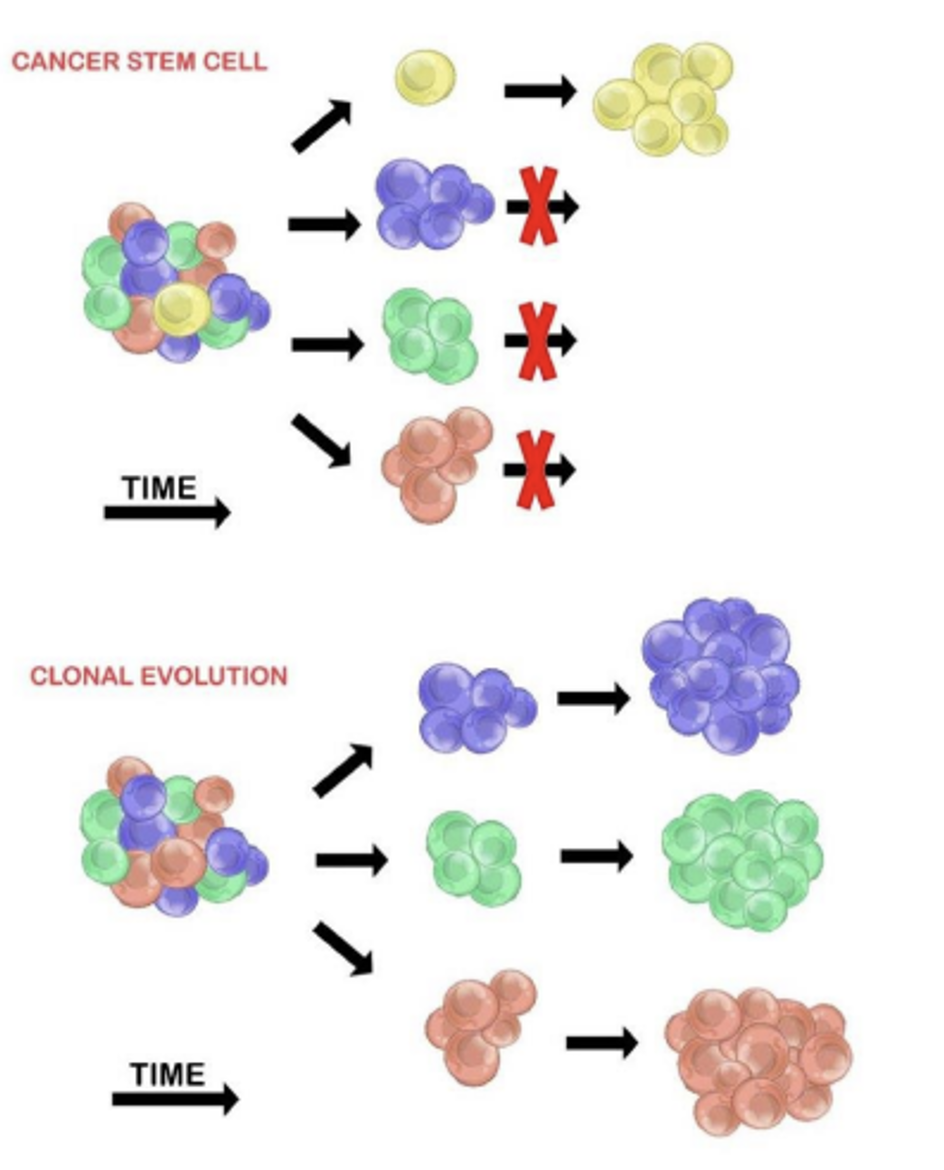
\includegraphics[width=10cm]{chaps/int/tumorheterogenety}}
	\caption{دو مدل برای ناهمگونی تومور}
	\label{fig:ch_intr:tumorheterogenety}
\end{figure}

یکی از توالی‌های پی در پی گسترش کلونی، یک مدل خطی از جانشینی کلونی است، جایی که جهش‌های متوالی پیدرپی باعث ایجاد توالی خطی از مجموعه‌های گسترش کلون می‌شوند و منجر به رشد کلون می‌شوند \cite{birbrair2014type}. مورد دیگر یک مدل چند کلونی از پیشرفت تومور است، که در آن یک سلول منفرد از طریق مکانیزم تقسیم به چندین زیرکلون گسترش می‌یابد \cite{lee2011promoter}. این مدل بیش از مدل خطی با ناهمگنی تومور مرتبط است. جهش‌های اکتسابی منجر به افزایش بی ثباتی ژنومی با هر نسل متوالی می‌شود \cite{cooper1992elements}. 

تومرهای
\gls{heterogenetic}
که متشکل از چندین کلون هستند، می‌توانند حساسیت‌های مختلفی را نسبت به \glspl{cytotoxic} در نشان دهند. علاوه بر این، می‌زان  ناهمگنی تومور می‌تواند خود به عنوان \gls{biomarker} مورد استفاده قرار گیرد زیرا هر چقدر می‌زان ناهمگنی تومور بیشتر باشد، احتمال حضور کلون‌های مقاوم در برابر درمان بیشتر است \cite{truninger2005immunohistochemical}. دلایل حساسیت‌های مختلف می‌تواند تعاملات بین کلون‌ها باشد که ممکن است اثر درمانی را مهار یا تغییر دهد \cite{birbrair2014type}. تومورهایی با ناهمگنی زیاد، با احتمال بیشتری از کلون‌های گوناگون تشکیل شده است که به درمان مقاوم هستند و ممکن است منجر به عدم موفقیت در درمان شوند. روش‌های نوین درمان تومور‌ها با هدف شخصی‌سازی برنامه‌های درمانی از طریق هدف قرار دادن جمعیت‌های سلولی توموری موجود در یک بیمار، توسعه می‌یابند \cite{fedele2014navigating}. ناهمگنی‌های توموری یکی از عوامل اصلی مقاومت در برابر دارو است و بنابراین، یک عامل بالقوه  در شکست درمان محسوب می‌شود. \cite{fedele2014navigating}. تومور‌ها می‌توانند از راه‌های مختلف به طور همزمان به مقاومت دارویی دست یابند، بنابراین هدف قرار دادن فقط یک مکانیسم مقاومت برای غلبه بر نارسایی درمانی، می‌تواند مزیت درمان‌های هدفمند را محدود کند\cite{burrell2014tumour}. بنابراین، ناهمگنی تومور می‌تواند برای درک توسعه تومور، پیچیدگی ایجاد کند و توسعه روش‌های موفقیت آمیز را با چالش روبرو کند \cite{fedele2014navigating}. مطالعه ناهمگنی تومور می‌تواند منجر به پیشرفت و توسعه روش‌های درمانی شخصی سازی شده شوند و درک ما را از روابط عملکردی بین کلون‌ها در طول درمان افزایش دهند\cite{burrell2014tumour}. برای مطالعه ناهمگنی تومور، بسیاری از ابزار‌های محاسباتی موثر برای تجزیه و تحلیل اطلاعات کلونی تومور و تاریخچه تکامل آن تولید شده است. این ابزار‌ها با استفاده از داده‌های تغییرپذیری ژنتیکی، تولید شده توسط فناوری‌های توالی یابی نسبتاً دقیق، قادر هستند تا ترکیب‌های کلونی تومور و رابطه اجداد بین کلون‌ها نتیجه دهند. این اطلاعات برای درک پیشرفت تومور و کمک به پیشرفت‌های درمانی کارآمد مهم است. 


در ادامه مفاهیم حوزه تحقیق مثل مدل‌های ناهمگنی توموری، روش‌های مختلف توالی‌یابی، ‌روش‌های مختلف ساخت درخت فیلوژنی تومور، مباحث مرتبط به یادگیری عمیق و یادگیری تقویتی به اختصار توضیح داده شد. در فصل سوم تحقیق پیشرو، به بررسی الگوریتم‌هایی که با استفاده از داده‌های توالی‌یابی تکسولی، درخت فیلوژنی تومور را استنباط کرده‌اند پرداخته شد. هر یک از این روش‌ها برای ساخت درخت فیلوژنی به همراه دادگان مورد استفاده، مورد ارزیابی قرار گرفت و در انت‌های فصل سوم مقایس‌های بین روش‌های مختلف صورت گرفت. در فصل چهارم روش پیشنهادی استنباط درخت فیلوژنی بر مبنای یادگیری تقویتی و داده‌های توالی‌یابی تکسولی به تفصیل بیان شده و در فصل پایانی نتایج بدست آمده و مقایسه آن با نتایج پیشین، گزارش شده است. در پایان موضوعات پیشنهادی که در کار‌های آتی در راستای ادامه این پژوهش می‌تواند مورد بررسی قرار گیرند، توضیح داده شد. 






		% فصل اول: مقدمه
% !TeX root=../../../main.tex

\chapter{مبانی تحقیق}
% دستور زیر باعث عدم‌نمایش شماره صفحه در اولین صفحهٔ این فصل می‌شود.
%\thispagestyle{empty}

در این فصل ابتدا مفاهیم مورد نیاز جهت تعریف مسئله مانند مدل‌های ناهمگنی تومور، روش‌های یافتن درخت تکاملی تومور، روش‌های توالی‌یابی داده مورد بررسی قرار می‌گیرند. در ادامه مدل‌های مورد استفاده برای استنباط درخت تکاملی تومور معرفی می‌شوند. در پایان مفاهیم مرتبط با یادگیری ماشینی، یادگیری عمیق و یادگیری تقویتی به منظور استنباط درخت تکاملی تومور با \gls{datadriven}  توضیح داده می‌شوند.


\section{تنوع ژنتیکی}

\gls{dna} 
یک مولکول بیولوژیکی است که توسط \glspl{nucleotid}  پلیمری شده است. در \gls{dna} چهار نوع \gls{nucleotid} وجود دارد: \gls{adenine}  (\lr{A})، \gls{thymine}  (\lr{T})، \gls{cytosine} (\lr{C}) و
 \gls{guanine} (\lr{G}).
  \gls{dna} اساس توالی اسیدهای آمینه است که پروتئین را تشکیل می‌دهد. یک مولکول \gls{dna} از دو رشته تشکیل شده است. که در \glspl{antiparallel}  هم و درجهت‌های مخالف قرار دارند و ساختاری از مارپیچ دوتایی ایجاد می‌کنند. هر نوع \gls{nucleotid} روی یک رشته با نوع دیگری از \gls{nucleotid} در رشته دیگر مرتبط است: A با T ؛ C با G (شکل \ref{fig:ch_lr:DNA_double_helix}) \cite{alberts2002molecular}. این به عنوان قانون پایه جفت شدن نوکلئوتید‌ها در هر رشته از \gls{dna} شناخته می‌شود.


\begin{figure}[!ht]
	\centerline{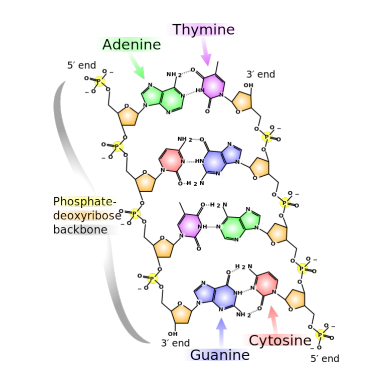
\includegraphics[width=11cm]{chaps/lr/DNA_double_helix}}
	\caption{مارپیچ دوگانه \gls{dna}}
	\label{fig:ch_lr:DNA_double_helix}
\end{figure}



همانند سازی \gls{dna} فرآیند تولید دو مولکول \gls{dna} یکسان از مولکول \gls{dna} اصلی است. وقتی تکثیر شروع می‌شود، دو رشته یک مولکول \gls{dna} از یکدیگر جدا می‌شوند و هر رشته به عنوان الگویی برای ساخت نمونه مشابه خود عمل می‌کند. نوکلئوتید‌ها در هر موقعیت از یک رشته با نوع دیگری از \gls{nucleotid} مبتنی بر قانون پایه جفت شدن، به منظور سنتز همتای این رشته، متصل می‌شود. پس از همانند سازی، مولکول \gls{dna} اصلی به دو مولکول یکسان تبدیل می‌شود (شکل \ref{fig:ch_lr:DNA_replication}) \cite{alberts2002molecular}.

\begin{figure}[!ht]
	\centerline{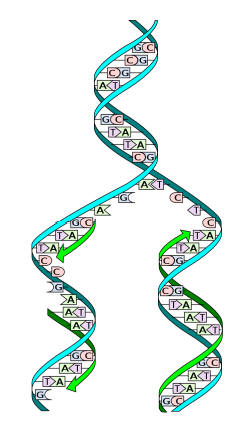
\includegraphics[width=8cm]{chaps/lr/DNA_replication}}
	\caption{همانندسازی \gls{dna}}
	\label{fig:ch_lr:DNA_replication}
\end{figure}





ژن ناحیه‌ای از \gls{dna} است و به عنوان مولکول واحد وراثت شناخته می‌شود. ژن‌های متعددی در ساختار \gls{dna} با عملکرد‌های متفاوت وجود دارد. جهش به تغییر دائمی‌توالی هسته‌ای ژنوم اتلاق می‌شود. جهش‌ها می‌توانند در حین فرآیند تکثیر \gls{dna} و با جفت‌گیری اشتباه در قسمت‌های مختلف \gls{dna} ایجاد می‌شود. انواع مختلفی از جهش‌ها مانند \gls{snm}(\gls{pointmutation})  (شکل \ref{fig:ch_lr:single_nucleotide_mutation}) و  \glspl{singlevariant}  شامل \gls{insertion} ، \gls{deletion}  و \gls{reversion}  (شکل \ref{fig:ch_lr:structural_changes}) وجود دارد. جهش‌های سلولی می‌توانند به بنا بر دلایلی چون مواد شیمیایی، سمیت یا ویروس ایجاد شوند. جهش در یک ژن می‌تواند محصولات آن را تغییر دهد (مانند ایجاد پروتئین متفاوت) یا از عملکرد صحیح ژن جلوگیری کند \cite{alberts2002molecular}.




\begin{figure}[!ht]
	\centerline{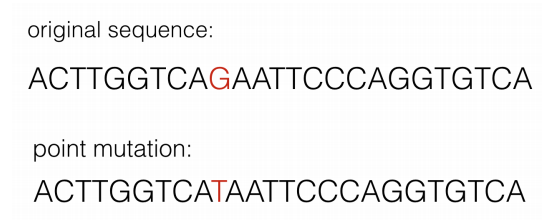
\includegraphics[width=10cm]{chaps/lr/single_nucleotide_mutation}}
	\caption{جهش تک‌نوکلئوتیدی}
	\label{fig:ch_lr:single_nucleotide_mutation}
\end{figure}



\begin{figure}[!ht]
	\centerline{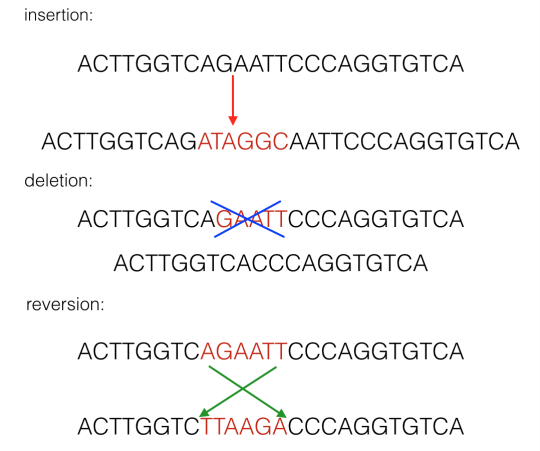
\includegraphics[width=10cm]{chaps/lr/structural_changes}}
	\caption{تغییرات ساختاری}
	\label{fig:ch_lr:structural_changes}
\end{figure}




\section{\gls{tumorevolution}}


جهشی که در هر سلول از بدن اتفاق می‌افتد، به استثنای سلول‌های جنسی (اسپرم و تخمک)، جهش \gls{somatic}  نامیده می-شود \cite{somaticMutation}. تجمع جهش بدنی در طول زندگی یک فرد می‌تواند منجر به رشد کنترل نشده مجموعه‌ای از سلول(تومور) شود \cite{nowell1976clonal} و می‌تواند باعث شکل‌گیری سرطان یا بیماری‌های دیگر شود \cite{somaticMutation}. بدلیل تجمع سلول‌های گوناگون، بیش از یک نوع سلول در تومور وجود خواهد داشت. به گروه‌های سلول با مجموعه‌ای از جهش مشخص، کلون یا جمعیت سلولی تومور گفته می‌شود. کلون‌های موجود در تومور از نظر فیلوژنتیک با هم مرتبط هستند و رابطه آنها را می‌توان با یک درخت فیلوژنتیک نشان داد \cite{birbrair2014type}. درخت فیلوژنتیک رابطه تکاملی بین کلون و ترتیب وقوع هر جهش را نشان می‌دهد. به عنوان مثال، شکل\ref{fig:ch_lr:tumor_phylogenetic_tree} :

\begin{itemize}
	\item یک درخت فیلوژنتیک از یک تومور با چهار کلون با برچسب $0$ تا $3$ را نشان می‌دهد.
	\item جهش جدیدی را نشان می‌دهد که در هر کلون در طول تکامل این تومور رخ داده است.
\end{itemize}

 همچنین هر کلون جهشی را در مسیر از کلون بالایی به سمت خود به ارث می‌برد. به عنوان مثال، کلون $0$ جهش‌های
  $m_0$ و	 $m_1$ دارد. کلون $1$ دارای جهش $m_0$، $m_2$، $m_3$ و $m_4$ است.
 
\begin{figure}[!ht]
	\centerline{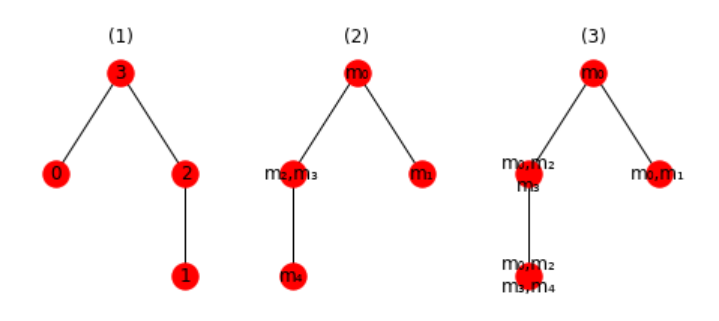
\includegraphics[width=13cm]{chaps/lr/tumor_phylogenetic_tree}}
	\caption{درخت فیلوژنیک تومور}
	\label{fig:ch_lr:tumor_phylogenetic_tree}
\end{figure}


\section{تکنولوژی‌های توالی‌یابی و \gls{variantallelefrequency}}




تعیین توالی \gls{dna} روشی برای تشخیص ترتیب دقیق \glspl{nucleotid} در یک رشته \gls{dna} است. روش \gls{nextgenerationsequencing}  از تعدادی فناوری مدرن توالی تشکیل شده است که امکان تعیین هزینه و زمان توالی‌یابی را به طور موثر فراهم می-کند. با استفاده از نمونه بیولوژیکی به عنوان ورودی این تکنولوژی‌ها، توالی‌های کوتاه نوکلئوتیدی تولید می‌شود (که به آن \gls{read}  گفته می‌شود). سپس خوانش با استفاده از الگوریتم \gls{alignment}  متنوعی مانند الگوریتم تبدیل \lr{Burrows-Wheeler} با ژنوم مرجع تراز می‌شوند. پس از ترازبندی، می‌توان با جمع‌آوری \glspl{overlappingread}،  توالی \gls{consensus}  ایجاد کرد (شکل \ref{fig:ch_lr:alignment_reading}). در موقعیتی از توالی اجماع به دلیل همپوشانی خوانش ها، ممکن است بیش از یک نوع خوانش از \gls{nucleotid} تراز شده وجود داشته باشد (تعداد کل قرائت مرتبط با یک نوع جهش، را \gls{readcoverage}  نامیده می‌شود). \gls{nucleotid} موجود در این موقعیت به عنوان رایج‌ترین \gls{nucleotid} تراز شده، مشخص می‌شود. به عنوان مثال، در شکل \ref{fig:ch_lr:alignment_reading}، سه آدنین (A)، یک گوانین (G) و یک تیمین (T)  در موقعیت سوم توالی اجماع تراز می‌شوند، سپس \gls{nucleotid} در آن موقعیت به عنوان آدنین (A) تعیین می‌شود. پس از ایجاد توالی اجماع، نوکلئوتیدهای موجود در آن توالی، که متفاوت از ژنوم مرجع هستند، شناسایی شده و به عنوان \gls{somaticsnv}  شناخته می‌شود. با استفاده از نمونه‌های متعدد استخراج شده از یک نمونه تومور، ما می‌توانیم تغییرات بدنی تک نوکلئوتیدی را در هر نمونه با فناوری تعیین توالی‌یابی تشخیص دهیم. نسبت تعداد سلول‌های موجود در یک نمونه حاوی تغییرات بدنی تک نوکلئوتیدی به کل سلول‌ها، فراوانی تغییرات آلل یک تغییر بدنی تک نوکلئوتیدی در این نمونه نامیده می‌شود. مقادیر فراوانی تغییرات آلل برای هر تغییر بدنی تک نوکلئوتیدی  در هر نمونه تومور قابل محاسبه است. ابزارهای زیادی برای بازسازی درخت فیلوژنتیک تومور از مقادیر فراوانی تغییرات آلل تومور به عنوان ورودی الگوریتم استفاده می‌کنند.



\begin{figure}[!ht]
	\centerline{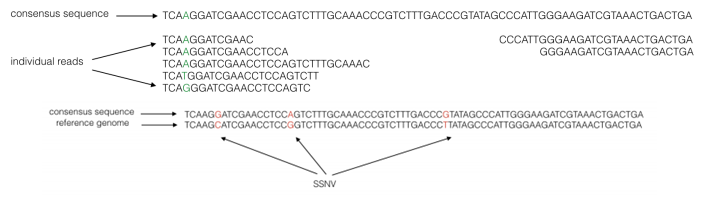
\includegraphics[width=\textwidth]{chaps/lr/alignment_reading}}
	\caption{تشخیص تغییر بدنی تک‌نوکلئوتیدی از طریق خوانش هم‌ترازی}
	\label{fig:ch_lr:alignment_reading}
\end{figure}



\section{ناهمگنی ژنومی تومور}

سرطان بیماری‌ای است که بدلیل ایجاد ناهنجاری‌های اساسی در فرآیند‌های بنیادی سلول مانند \gls{replication}، \gls{differentiation}  و \gls{death} سلول  ایجاد می‌شود \cite{hanahan2011hallmarks}. این ناهنجاری منجر به رشد کنترل نشده تومور و به‌کارگیری بافت غیرسرطانی برای حمایت از این رشد می‌شود. علت اصلی این تغییرات جهش است. جهش یک اصطلاح گسترده است که چندین دسته از تغییرات ژنتیکی را پوشش می‌دهد. هنگام حاملگی، یک جنین دارای یک ژنوم خاص و منحصر به فرد است. این ژنوم که به \gls{germlinegenome} معروف است، می‌تواند با ژنوم انسانی مرجع مقایسه شود. ژنوم انسانی مرجع یک نمونه از ژنوم انسان است و از \gls{dna} چند نفر تشکیل شده است. تفاوت بین ژنوم جوانه‌زنی و ژنوم مرجع به عنوان جهش ژنوم جوانه زنی شناخته می-شود. جهش‌های جوانه زنی می‌توانند مسئول افزایش خطر ابتلا به سرطان باشند \cite{stewart2017world}، اما بندرت خود مسئول مستقیم توسعه تومور هستند. 




معمولاً تومورها در اثر جهش‌های اکتساب شده پس از لقاح، که معروف به جهش‌های بدنی هستند، ایجاد می‌شوند. جهش-های بدنی نتیجه اشتباهات در تکثیر \gls{dna} \cite{behjati2014genome}، قرار گرفتن در معرض جهش‌های با منشأ داخلی یا خارجی یا وارد‌شدن توالی‌های \gls{dna} با منشأ بیرونی بدلیل قرار گرفتن در معرض ویروس است \cite{talbot2004viruses}. غالباً در سرطان، جهش‌های بدنی باعث ایجاد اختلال در روند تکثیر \gls{dna} یا ترمیم آن می‌شوند و حتی جهش‌های بدنی بیشتری ایجاد می‌کنند \cite{stratton2009cancer}. نظریه کلونی بودن سرطان \cite{nowell1976clonal} سرطان را به عنوان یک تک سلولی با منشأ غیرجنسی در نظر می‌گیرد که در اثر تولید مثل فراوان، یک توده متشکل از کلون‌های سلولی گوناگون را ایجاد می‌کند. در این مدل سلولهای توموری با یکدیگر در رقابت هستند و جهش‌های بدنی که مزیت رشد را ایجاد می‌کنند در جمعیت سلول‌های توموری از نسبت بیشتری برخوردار خواهند بود. جهش‌های بدنی که باعث رشد تومور شده و از سلولی به سلولی دیگر منتقل می‌شوند به عنوان \glspl{drivermutation} شناخته می‌شوند. اولین سلولی که دارای جهش راننده بوده و آن را به جهش‌های بعدی منتقل می‌کند به عنوان سلول بنیانگذار شناخته می‌شود. همه فرزندان این سلول بنیانگذار، جهش راننده و هر جهش دیگری را که سلول بنیانگذار قبل از به دست آوردن جهش راننده بدست آورده است، دارند. این جهش‌های دیگر، که مزیتی برای رشد و گسترش تنوع توموری ندارند، به عنوان \glspl{passengermutation} شناخته می‌شوند. شایان ذکر است که تعریف جهش راننده و مسافر به زمینه ژنتیکی و محیطی بستگی دارد. به عنوان مثال، شیمی درمانی \gls{cytotoxic}  (سیتوتوکسیک) می‌تواند باعث تغییر جهش از مسافر به جهش راننده شود و عامل اصلی مقاومت در برابر درمان باشد. همچنین جهش ها را می‌توان بر اساس نوع تغییری که در \gls{dna} ایجاد می‌شود، به طبقات متمایز تقسیم کرد. \gls{snv} جهش‌هایی هستند که یک پایه در ژنوم را به پایه دیگری تغییر می‌دهند. \gls{indel}  درج یا حذف یک بخش \gls{dna} است که می‌تواند کوتاه یا طولانی باشد. از ایندل کوتاه و تغییرات تک نوکلئوتیدی در مجموع به عنوان \glspl{ssm}  یاد می‌شود. در همه قسمت‌های یک ژنوم، از جمله کل کروموزوم‌ها، قابلیت حذف یا کپی شدن قسمتی از ژنوم وجود دارد. تغییرات شماره کپی  به جهشی اتلاق می‌شود که منجر به حذف یا کپی شدن قسمتی از ژنوم می‌شود. \gls{cna} نوعی \gls{singlevariant} هستند که شامل وارونگی (وقتی قسمت بزرگی از ژنوم معکوس شده باشد) و انتقال متعادل (جایی که دو بخش ژنومی مکان‌‌های خود را با یکدیگر تعویض می‌کنند) می‌باشند\cite{stratton2009cancer}. این گونه‌های مختلف جهش مستقل از یکدیگر نیستند و می‌توانند در رابطه با یکدیگر اتفاق بیفتند (به عنوان مثال یک جهش می‌تواند منجر به تقویت یک وارونگی شود). 



تکنیک توالی‌یابی نسل بعدی این امکان را فراهم کرده است تا با صرف هزینه بسیار کم و با استفاده از یک نمونه توموری، توالی‌یابی از \gls{dna} صورت پذیرد و همین امر منجر به تحول گسترده‌ای در زمینه مطالعه تکامل تومور شده زیر امکان نمونه-برداری در تعداد بسیار بالا را از تومور فراهم می‌کند. نمونه‌گیری در حجم بالا این امکان را فراهم آورده است تا ناهمگنی تومور از نقطه منظر ژنتیکی مورد بررسی قرار گیرد و پاسخ به درمان بیماران سرطانی با جزییات بیشتری مورد ارزیابی قرار گیرد.


تقریباً همه نمونه‌های استخراج شده از تومور ترکیبی از سلول ها با ژنوتیپ‌های مختلف را شامل می‌شود. یک نمونه توموری به ندرت فقط شامل بافت سرطانی است زیرا شامل سلول‌های غیر سرطانی از \gls{surroundingstroma}  یا \glspl{Infiltratingimmunecell}  است. مطالعات ژنومیک نشان داده است که حتی در میان سلولهای سرطانی، غالباً زیرجمعیت‌های متعدد سرطانی نیز وجود دارد. به عنوان مثال، در یک مطالعه مهم در سال 2012، گرلینگر و همکارانش \cite{gerlinger2012intratumor} توالی‌یابی ژنوم و تغییرات شماره کپی را از طریق نمونه‌های مکانی مجزا استخراج شده از سرطان کلیه اولیه و نقاط متاستاز ثانویه بدست آورده‌اند. با بررسی  این نمونه‌های متعدد، مشخص شد که یک ناهمگنی ژنتیکی قابل توجهی در تومور وجود دارد. تعداد بسیار زیادی از جهش‌های شناسایی شده در همه سلول‌های توموری مشاهده نشدند و این بدان معناست که این جهش‌ها بیش از آن‌که یک ناحیه کلونی باشند، به صورت یک ناحیه زیر کلونی بوده‌اند. با استفاده از روش‌های پردازش غیراتوماتیک، تغییرات تک نوکلئوتیدی  ها و تغییرات شماره کپی بر اساس نمونه‌هایی که از آن استخراج شده‌اند، به خوشه‌های مجزا دسته‌بندی شده و یک درخت فیلوژنی به آن‌ها نسبت داده شد. بازسازی درخت فیلوژنیک تومور این امکان را فراهم آورد تا سیر تکاملی تومور با استفاده از شاخه‌های مختلف درخت فیلوژنی شامل جهش‌هایی با عملکرد یکسان از سه ژن متفاوت مورد بررسی قرار گیرد. 


در همان سال، یک مطالعه مهم دیگر، "تاریخچه زندگی 21 سرطان پستان`` \cite{nik2012life}، حضور \lr{ITH} را نیز نشان داد. در این مطالعه آنها توالی‌یابی کامل ژنوم را در عمق متوسط \lr{188X} بر روی تومور پستان \lr{PD4120a} انجام دادند. این عمق اجازه می‌دهد تا جمعیت‌های شیوع تا 5٪ کم باشد. آنها مشاهده کردند که تغییرات تک نوکلئوتیدی‌ها در تعداد کمی از خوشه‌های مجزا مشاهده می‌شوند که با توجه به کسر نوع آلل (\lr{VAF}) آنها مشاهده می‌شود، نسبت خواندن ها در یک مکان متفاوت شامل آلل نوع. علاوه بر این، آنها توانستند نشان دهند که برخی از این خوشه‌های مجزا را نمی‌توان با جهش‌های موجود در تمام جمعیت‌های سرطانی توضیح داد، که این نشان دهنده حضور تغییرات تک نوکلئوتیدی‌های تحت کلونال است. در همان زمان، آنها دریافتند که بسیاری از جهش‌ها در تمام سلول‌های سرطانی موجود در نمونه وجود دارد، که نشان می‌دهد جد مشترک اخیر نسبتاً دیر در زمان تکامل رشد کرده است. مشاهده اینکه جهش‌های زیر کلونال به جای توزیع یکنواخت یا مطابق قانون قدرت در خوشه‌های متمایز پیدا شده است، شواهدی را نشان می‌دهد که این جهش‌های زیرکلونالی بیش از آنکه ناشی از تکامل خنثی یا مصنوعات فنی باشد، در زیرمجموعه‌های متمایز ناشی از فشارهای انتخابی یافت می‌شود. نویسندگان همچنین با تأیید اینکه جهش‌های زیر کلونال محدود به تغییرات تک نوکلئوتیدی  نیستند، توانستند حضور تغییرات شماره کپی‌های کلونال و زیرکلونال را تأیید کنند. نویسندگان یک الگوریتم خوشه‌بندی غیر پارامتریک (یک مدل مخلوط فرآیند دیریشله (\lr{DPMM})) را با استدلال قابل توجه دستی برای استنباط فیلوژنی شاخه‌ای از چهار زیر جمعیت سرطانی در آن نمونه منفرد تومور ترکیب کردند. درک معماری ژنتیکی این زیرجمعیت‌ها می‌تواند به مطالعه زیست شناسی سرطان کمک کند و نشان داده شده است که در پیش‌بینی بقا در بسیاری از انواع سرطان مفید است \cite{andor2016pan}. به عنوان مثال، زیرجمعیت‌های مختلف، که توسط مجموعه جهش‌های جسمی حمل شده تعریف می‌شوند، توانایی‌های مختلفی در مقاومت در برابر درمان و متاستاز دارند. برای انجام این کار، باید از یک یا تعداد کمی از نمونه‌های تومور فله، ژنوتیپ‌های موجود در نمونه را شناسایی کرد. این مسئله، تحت عنوان بازسازی ساب کلونال، موضوع اصلی این پایان‌نامه است. مطالعات پیشگام که نشان داد \lr{ITH} برای انجام این بازسازی به استدلال دستی قابل توجهی نیاز دارد. استدلال دستی کند، مستعد خطا است و به تخصص قابل توجهی نیاز دارد. مزایای بازسازی کاملاً خودکار بدیهی است. این بخش پیش زمینه مشکل بازسازی زیر کلونال، چگونگی پرداختن به آن برای انواع مختلف جهش، خصوصیات اصلی الگوریتم‌های بازسازی زیر کلونال و خلاصه‌ای از کارهای موجود در این زمینه را توصیف می‌کند.


\section{بازسازی زیر کلونال }

بازسازی ساب کلونال سعی دارد ژنوتیپ‌های موجود در تومور را از تعداد کمی از نمونه‌های توالی \gls{dna} از آن تومور استنباط کند. تعداد ژنوتیپ‌های موجود در تومور از قبل مشخص نیست. این ژنوتیپ‌های زیر کلونال به طور معمول با جهش‌هایی که در مقایسه با ژنوم خط جوانه‌ای دارند، توصیف می‌شوند. ژنوم جوانه‌زنی علاوه بر نمونه(های) تومور، با تعیین توالی یک نمونه غیرسرطانی تعیین می‌شود. در حال حاضر در هنگام تعریف این جمعیت از دو نوع جهش به طور معمول استفاده می‌شود: جهش‌های ساده بدنی‌های متشکل از تعویض‌ها و درج / حذف کوچک (ایندل) و \gls{cna} حاصل از تغییرات ساختاری بزرگتر. مشاهده انواع جهش‌های دیگر، مانند مجموعه گسترده‌ای از \lr{SV}‌ها که شامل بازآرایی هستند، مشاهده آنها دشوارتر است و روش‌های شناسایی آنها در مراحل اولیه رشد است.


به طور متوسط، حتی در شرایط ایده آل، هر سلول در هر بخش یک جهش پیدا می‌کند \cite{behjati2014genome}، به همین ترتیب، بیشتر سلول‌های تومور ژنوتیپ منحصر به فردی خواهند داشت. بنابراین، به طور دقیق، اکثر سلولهای تومور می‌توانند به طور بالقوه نمایانگر زیرجمعیت منحصر به فرد خود باشند. با این حال، به طور عملی، جهش‌هایی که مختص سلول‌های منفرد است یا فقط تعداد کمی از سلول‌ها آنها را به اشتراک می‌گذارد، در حین فراخوانی نوع شناسایی نمی‌شوند. تماس متغیر در بخش 2.5.3 بیشتر مورد بحث قرار گرفته است. بعلاوه، سلول‌هایی که بخش عمده‌ای از جهش‌های خود را به اشتراک می‌گذارند، خصوصاً جهش‌های راننده، صفات مشابهی دارند. به همین ترتیب، من قرارداد گسترده‌ای را اتخاذ کرده و یک زیر جمعیت را به عنوان تمام سلول‌هایی که دارای زیر مجموعه یکسان جهش‌های بدنی در هنگام فراخوانی نوع هستند، تعریف می‌کنم.


یک گام مهم در بازسازی ساب کلونال محاسبه شیوع سلولی تبارهای زیر کلونال و سپس، در نهایت، زیرجمعیت‌های سرطانی است. شیوع سلولی یک زیرجمعیت، نسبت سلول‌های نمونه توالی شده متعلق به آن است. غالباً، شیوع سلولی با تقسیم بر خلوص نمونه، یعنی نسبت سلولهای سرطانی در نمونه، به بخش سلولهای سرطانی، نسبت سلولهای سرطانی، تبدیل می‌شود. هر سلول دقیقاً به یک زیرمجموعه تعلق دارد، بنابراین این شیوع باید در یک جمع باشد. به طور کلی، سلول‌های غیر سرطانی در یک زیرمجموعه واحد قرار می‌گیرند. با این حال، از آنجا که جهش‌ها اغلب در زیرجمعیت‌های متعدد وجود دارند، شیوع سلولی بسیاری از زیرجمعیت‌ها را نمی‌توان مستقیماً از جهش‌های آن استنباط کرد. برای پرداختن به این موضوع، ما یک نسب زیر کلونال برای یک جهش به عنوان مجموعه زیرجمعیت‌هایی که در آن وجود دارد، تعریف می‌کنیم. به طور رسمی، دودمان‌های زیر کلونال از زیر جمعیت بنیانگذار تشکیل می‌شود (جایی که جهش برای اولین بار ظاهر می‌شود) و همه زیرجمعیت‌های بعدی آن (که وراثت جهش) علاوه بر جهش‌های خاص خود، این زیرمجموعه‌های فرزندی حاوی تمام جهش‌های موجود در نژاد تعریف کننده زیر جمعیت هستند (به جز در صورت حذف محل منبع جهش، برای جزئیات بیشتر به فصل 3 مراجعه کنید). نسب مربوط به یک زیر درخت (یا کلاد) از درخت کلون تومور است. شیوع سلولی یک تبار مجموع شیوع سلولی زیرجمعیت‌هایی است که متعلق به آن تبار هستند. از آنجا که سلول‌ها می‌توانند در چندین نژاد زیرکلونال وجود داشته باشند، شیوع نسب در یک جمع نیست.



شکل \ref{fig:ch_lr:tumor_clone_tree} تصویری از یک درخت کلون نمونه را ارائه می‌دهد. گره‌های موجود در درخت، همانطور که در بالا تعریف شد، نشان دهنده زیر جمعیت است. فلش‌ها از جمعیت والدین به سمت فرزندانشان هدایت می‌شوند. دودمانهای زیر کلونال به صورت مستطیل نشان داده می‌شوند و با توجه به زیرمجموعه بنیادی آنها که در ریشه تیغه یافت می‌شوند، رنگی هستند.


\begin{figure}[!ht]
	\centerline{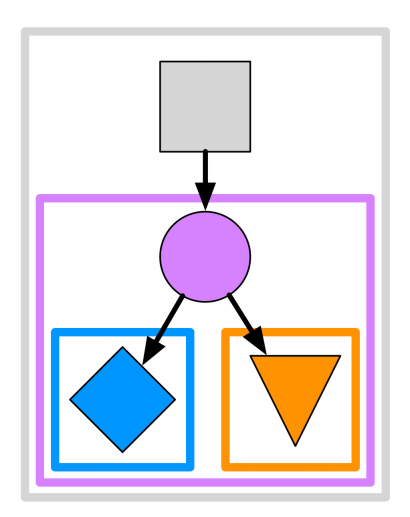
\includegraphics[width=7cm]{chaps/lr/tumor_clone_tree}}
	\caption{درخت کلون تومور}
	\label{fig:ch_lr:tumor_clone_tree}
\end{figure}




\section{تغییرات تعداد کپی}

بیشتر ژنوم انسان دیپلوئید است، به این معنی که دو نسخه از توالی \gls{dna} ما در سلول‌های ما وجود دارد، یکی از پدر و دیگری از مادر. تغییرات شماره کپی این تغییر را می‌دهند، یا با تغییر در تعداد نسخه‌ها (مثلاً از طریق تکثیر کل ژنوم)، نسبت کپی‌های مادر به پدر (مثلاً از دست دادن خنثی هتروزیگوزیته در تعداد کپی‌ها، جایی که برای همان منطقه یک ژنوم والدین تکثیر می‌شود و دیگری حذف شده است) یا هر دو (به عنوان مثال کپی کروموزوم مادر). بیشتر این تغییرات (به استثنای تکثیر کل ژنوم) دامنه محدودی از ژنوم را تحت تأثیر قرار می‌دهد، اما می‌تواند از تأثیر یک ژن تا یک کروموزوم کامل باشد. این بخش از ژنوم تغییر یافته به عنوان یک بخش شناخته می‌شود.


تغییرات شماره کپی می‌توانند تعداد کپی کل یک بخش و / یا تعداد نسبی نسبی دو کروموزوم والدین را تغییر دهند. هر یک از این تغییرات توسط توالی‌یابی ژنومی هسته قابل تشخیص است. تغییر در تعداد کپی کل یک بخش را می‌توان تشخیص داد زیرا نسبت خواندن آن نقشه به آن بخش بین خط جوانه زنی و نمونه تومور متفاوت خواهد بود. بخش از یک قطعه نسبت ورود خوانده شده است که به یک قطعه در یک نمونه غیر سرطانی ترسیم شده است به نسبت خوانده شده که به یک بخش در یک نمونه سرطانی ترسیم شده است. از نسبت نسبت‌ها برای محاسبه این واقعیت استفاده می‌شود که تعداد کل قرائت‌ها اغلب بین توالی‌یابی سرطانی و غیرسرطانی متفاوت است، در مناطق مختلف ژنوم عمق خواندن بیشتر یا پایین‌تر ناشی از محتوای \lr{GC} یا نقشه برداری وجود دارد و تردستی یک تومور با بافت طبیعی متفاوت است. تکرر یک ژنوم، میانگین تعداد کپی از هر کروموزوم است که برای طول کروموزوم نرمال می‌شود.


با تغییر در کسر آلل می‌توان عدم تعادل در تعداد نسخه‌های مادری و پدری این بخش را تشخیص داد. در مناطق دیپلوئید ژنوم‌ها، اگر یک بازه بین کپی‌های مادر و پدر متفاوت باشد، موقعیت هتروزیگوت نامیده می‌شود. جهش‌های تک پایه، خط جوانه زنی همچنین به عنوان چند شکلی تک هسته‌ای نامیده می‌شوند. وقتی یک ژنوم توالی‌یابی شود، حدود نیمی از قرائت آن مکان هتروزیگوت حاوی هر یک از بازها خواهد بود، در نتیجه کسر آلل 50 است. این امر تا زمانی که نسبتی برابر با نسخه‌های مادرانه و پدری وجود داشته باشد، صادق خواهد بود. اگر این نسبت تغییر کند، کسر آلل  تمام پولیمورفیسم تک هسته‌ای در بخش آسیب دیده تغییر می‌کند. پولیمورفیسم تک هسته‌ای هتروزیگوت به طور متوسط هر 1500 باز \cite{chen2012personal} رخ می‌دهد و بنابراین برای بخشهای طولانی بسیاری از پولیمورفیسم تک هسته ایی هتروزیگوت تحت تأثیر قرار می‌گیرند. توزیع کسر آلل \lr{S} تمام پولیمورفیسم تک هسته‌ای در بخش، حالت دوگانه‌ای پیدا می‌کند که هر حالت نشان دهنده نسبت نسخه‌های آن بخش از هر والد است.

فراخوانی \lr{CNA} چالش برانگیز است زیرا با مشاهده مستقل هر بخش، مسئله هنوز مشخص نشده است. حتی با فرض اینکه هر بخش فقط توسط یک \lr{CNA} تحت تأثیر قرار گیرد، \lr{CNA} موسوم به سه پارامتر (نسبت سلولهای حاوی \lr{CNA}، تعداد کپی‌های مادر و تعداد کپی‌های پدری) وجود دارد و فقط دو مشاهده برای توضیح وجود دارد (و کسر آلل )

همه روش‌ها با فرض اینکه تعداد کمی از نژادهای زیرکلونال مسئول بیشتر یا تمام تغییرات شماره کپی هستند، این ابهام را برطرف می‌کنند. روشی که توسط الگوریتم باتنبرگ \cite{nik2012life} به کار رفته است، به بیشتر تغییرات شماره کپی وابسته به یک نژاد زیر کلونال منفرد و شایع به نام تبار کلونال متکی است. تحت این روش، شیوع این تبار، همراه با تعداد کپی اصلی و جزئی در تمام تغییرات تعداد کپیکلونال، می‌تواند با یک فرآیند دو مرحله‌ای تخمین زده شود. در گام اول، این روش با فرض شیوع نژاد کلون $f_c$  آغاز می‌شود. شیوع تبار کلونال در بیشتر موارد با خلوص نمونه تومور برابر است. با توجه به شیوع کلونال، هر بخش پس از آن فقط دو متغیر برای توضیح دارد (تعداد کپی بزرگ و جزئی). از آنجا که هر بخش دارای دو مشاهدات است، اکنون مسئله هنوز به درستی تعیین نشده است و بهترین کپی اصلی و مینور متناسب است. سپس، ترکیب کلی مقدار $\Phi_c$  فرض شده با ترکیب مناسب در تمام بخشها تعیین می‌شود. الگوریتم با بهینه سازی این تناسب بهترین مقدار $\Phi_c$  را انتخاب می‌کند. سپس برای هر بخش، شماره کپی اصلی و جزئی با بهینه سازی متناسب بودن قطعه با بهترین مقدار $\Phi_c$   انتخاب می‌شود. این روش فرض می‌کند که تمام تغییرات شماره کپی به نژاد کلونال تعلق دارند، که همیشه درست نیست. در مرحله بعدی، بخشهایی که حاوی تغییرات تعداد کپیتحت کلونال هستند با جستجوی بخشهایی با اطلاعات مناسب ضعیف با استفاده از $\Phi_c$   استنباط شده مشخص می‌شوند. در این بخش‌ها، روش به طور همزمان و مستقل از هر بخش دیگر، عدد $\Phi_i$   و عدد کپی بزرگ و جزئی را استنباط می‌کند.


از آنجا که سه متغیر وجود دارد و تنها دو مشاهده وجود دارد، راه حل‌های بسیاری با تناسب داده برابر وجود دارد که از نظر زیست شناختی برای این تغییرات تعداد کپی زیر کلونال قابل قبول است. این ابهام با انتخاب راه حلی که نزدیکترین شماره به شماره نسخه طبیعی است برطرف می‌شود، اما تعدادی از موارد متداول وجود دارد که این ابتکار عمل ناموفق است. سپس این روش‌ها انتساب تغییرات تعداد کپی زیرکلونال به دودمان و تمام استنباط‌های فیلوژنتیک را برای روش‌های پایین دست رها می‌کنند.


رویکرد عمده دیگر این است که فرض کنیم همه تغییرات شماره کپی از تعداد کمی تبار ساب کلونال به وجود می‌آیند. الگوریتم‌هایی که از این روش استفاده می‌کنند به طور مشترک شیوع این نژادها و تعداد کپی بزرگ و جزئی را برای هر بخش استنتاج می‌کنند (به عنوان مثال \lr{THetA}\cite{zhu2011metabolic, vander2009understanding} و \lr{TITAN} ).  تعداد دودمانهای زیر کلونال معمولاً با استفاده از احتمال جریمه شده‌ای مانند معیار اطلاعات بیزی (\lr{BIC}) یا انواع \lr{BIC} تعیین می‌شود (به عنوان مثال \lr{THetA} از \lr{BIC} اصلاح شده با پارامتر مقیاس گذاری استفاده می‌کند \cite{zhu2011metabolic}). بنابراین این روش‌ها هم تغییرات شماره کپیرا فراخوانی می‌کنند و هم آنها را به دودمان‌های زیرکلونال اختصاص می‌دهند. هیچ روش موجود این دودمان‌ها را در یک درخت فیلوژنتیک قرار نمی‌دهد



\section{جهش‌های ساده بدنی }

جهش‌های ساده بدنی جهش‌های کوچکی هستند که می‌توانند مستقیماً از طریق توالی‌یابی و نسبت کروموزوم‌های موجود در نمونه حاوی آنها از تعداد قرائت‌های حاوی جهش و تعداد کل خوانده‌ها در آن مکان، مشاهده شوند. نسبت قرائت حاوی جهش به کل قرائت به عنوان \lr{VAF} جهش شناخته می‌شود. جهش‌های ساده بدنی‌ها معمولاً با بررسی مشترک ترازها و یک نمونه غیر‌سرطانی خوانده می‌شوند. این استنباط مشترک برای جداسازی انواع بدنی و ژرمینال مورد نیاز است.

این فرایند به دلیل انواع مختلف خطاها و تعصبات که در داده‌های \lr{NGS} وجود دارد، دشوار می‌شود\cite{friedl2010plasticity}. یک مشکل اساسی در تشخیص جهش‌های ساده بدنی این است که به نظر می‌رسد خطاهای توالی جهش‌های ساده بدنی شیوع کمی دارند. به طور خاص، در  \lr{Illumina Hiseq2000}  که به طور گسترده استفاده می‌شود، از هر 1000 پایه یکی از آنها دارای یک خطا است (به طور معمول یک تعویض) \cite{sabeh2009protease}. به همین ترتیب، در طول سه میلیارد پایه ژنوم انسانی، یک احتمال غیر قابل اغماض وجود دارد که در بعضی موقعیت‌ها، چندین بار خواندن دقیقاً شامل خطای توالی دقیقاً در همان موقعیت‌ها است. به نظر می‌رسد این خطاها شیوع کم جهش‌های ساده بدنی دارند. تمایز بین این خطاها و شیوع کم واقعی جهش‌های ساده بدنی‌ها شامل یک معامله بین حساسیت و ویژگی و در حالت ایده آل، یک مدل نویز بسیار دقیق است. حل این مشکل امتداد طبیعی کار گسترده‌ای است که در زمینه فراخوانی جهش‌های جوانه‌زنی انجام شده است و الگوریتم‌های زیادی برای انجام این کار وجود دارد (به عنوان مثال \cite{friedl2010plasticity, demicheli2008effects})


\section{\gls{allelecdropout}}

اگرچه روش‌های تعیین توالی با بازدهی بالا \cite{hugo2007epithelial} ارزان هستند، اما تحت تاثیر مقدار بایاس هستند و مارکرهای ژنتیکی‌ای تولید می‌کنند که تقریباً به طور تصادفی در کل ژنوم تقسیم می‌شوند. این روشها با موفقیت در \gls{mapping} صفات \cite{nowell1976clonal, greaves2012clonal}، ساخت مپ پیوندی \cite{sakr1993frequency, fearon1990genetic}،  اسکن انتخاب  \cite{dentro2018portraits, waclaw2015spatial}،  و برآورد تنوع ژنتیکی \cite{de2006clonal} استفاده شده است. یکی از این روش‌ها، تعیین ژنوتیپ براساس توالی \cite{anderson2011genetic} (\lr{GBS}) است. در \lr{GBS}، هدف توالی‌یابی فقط با اتصال آداپتورهای توالی به محل‌های برش آنزیم محدود کننده، به کمتر از $5\%$ از ژنوم کاهش می‌یابد (شکل زیر).  قرائت \lr{GBS} همچنین می‌تواند به صورت کانکت‌های کوتاه مونتاژ شود، که بدون نیاز به توالی ژنوم فراخوانی یک نوع تغییر تک هسته‌ای (تغییرات تک نوکلئوتیدی ) را امکان پذیر می‌کند \cite{hanahan2000hallmarks}. از این رو، \lr{GBS} یک روش محبوب در سیستم‌های غیر مدلی است که به طور معمول فاقد منابعی مانند مجموعه ژنوم و ریزآرایه‌ها است.

بر خلاف توالی‌یابی کل ژنوم \lr{(WGS)}، \lr{GBS} مستعد ابتلا به خطاهای مختلف تماس به دلیل محدودیت چندشکلی‌های سایت  است (کاهش آللیک). کاهش آللیک در \lr{GBS} می‌تواند برنامه‌هایی را که به فراخوانی دقیق تغییرات نادر، از جمله تخمین طیف فرکانس سایت در ژنتیک جمعیت متکی هستند، را دچار اختلال کند. یک رویکرد آماری سیستماتیک برای تشخیص کاهش آللیک در داده‌های توالی \lr{GBS}، اجرا شده و  در بسته نرم افزاری منبع باز \lr{GBStools} وجود دارد.  این روش مبتنی بر این واقعیت است که کاهش آللیک متناسب با تعداد آللهای سایت محدود کننده بدون برش که در آنجا حمل می‌کند، میزان خوانش نمونه را در یک سایت خاص کاهش می‌دهد. بنابراین \lr{GBStools} پوشش هر نمونه را در یک سایت خاص به عنوان یک متغیر تصادفی پواسون مورد استفاده قرار می‌دهد که از توزیع با میانگین \lr{$\lambda$} (آللیک‌های بدون برش صفر)، توزیع با میانگین ½\lr{$\lambda$} (یک آللیک بدون برش)، یا با میانگین صفر (دو آللیک بدون برش). \lr{GBStools} حداکثر احتمال پارامتر \lr{$\lambda$} را با استفاده از تعداد واقعی آللیک‌های بدون برش در هر نمونه که به عنوان متغیرهای نهفته (مشاهده نشده) در نظر رفته می‌شود و از طریق  حداکثر رساندن  مقدار چشم انتظاری \lr{(EM)}، محاسبه می‌کند . از مقادیر مورد انتظار این متغیرهای نهفته می‌توان برای تخمین اینکه کدام نمونه ها یک آللیک بدون برش دارند استفاده کرد. به طور همزمان، \lr{GBStools} فرکانس سایت آلل‌های \lr{SNP} مرجع قابل مشاهده و جایگزین، \lr{$\varphi_1$} و  \lr{$\varphi_2$}  ، و آللیک بدون برش، \lr{$\varphi_3$} ، که در آن  \lr{$\varphi_1$+$\varphi_2$+$\varphi_3$=1}   برآورد می‌کند و در نهایت، آزمون نسبت احتمال با مقایسه فرضیه صفر  \lr{$\varphi_3$ = 0} با فرضیه \lr{$\varphi_3$> 0} جایگزین می‌کند. \lr{GBStools}  در اجرای فعلی خود نمی تواند ژنوتیپ‌های واقعی پنهان شده توسط کاهش آللیک را استنباط کند، اما می‌توان با فیلتر کردن سایت‌هایی که نسبت احتمال آنها زیاد است خطاها را حذف کند.

\begin{figure}[!ht]
	\centerline{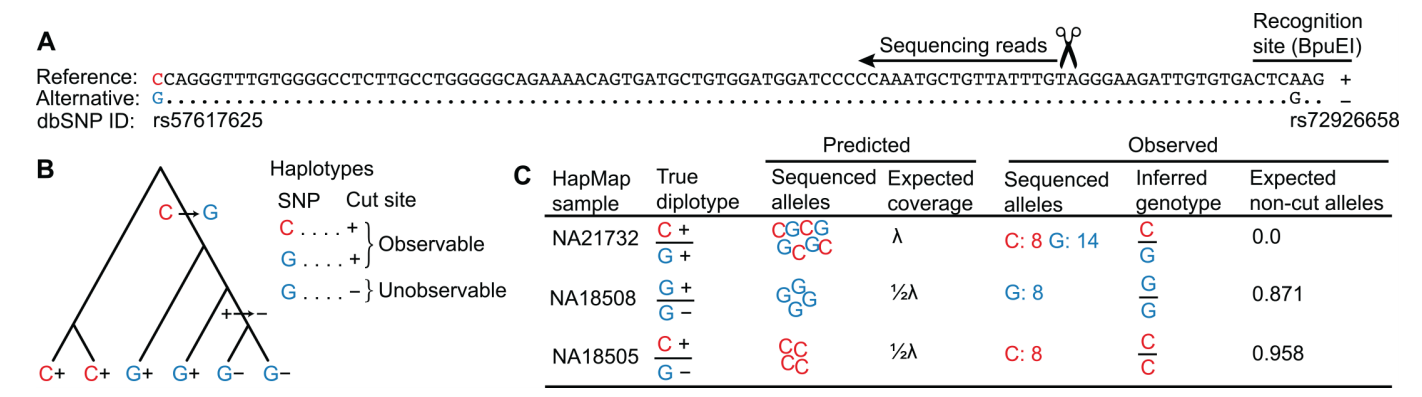
\includegraphics[width=\textwidth]{chaps/lr/mtsd}}
	\caption{نمایی از تطابق ژنتیکی}
	\label{fig:ch_lr:mtsd}
\end{figure}

در شکل بالا، آلل \lr{BpuEI} بدون برش ناشی از \lr{SNP rs72926658} با برچسب "-`` و آلل برش با "+`` برچسب گذاری شده است. آلل "-`` در هاپلوتیپ با آلل \lr{G} مشتق شده بوجود آمده و باعث شده تا برخی از آلل‌های \lr{G} توسط \lr{GBS} قابل مشاهده نباشند. نمونه‌های نشان داده شده دارای سه دیپلوتیپ هتروزیگوت است. نتایج توالی با پیش‌بینی‌ها مطابقت داشت و نمونه \lr{NA18505} به اشتباه هموزیگوت نامیده می‌شد، اما انتظار می‌رود تعداد آلل‌های کاهشی محاسبه‌شده توسط \lr{GBStools (0.958)} با تعداد واقعی (1) مطابقت داشته باشد، و آن را به عنوان یک تماس اشتباه احتمالی مشخص کند.

\section{مقدمه‌ای بر مدل‌سازی احتمالی }

وظیفه اصلی یادگیری ماشین، یادگیری از داده‌ها است، کاری که به عنوان استنباط شناخته می‌شود. برای یادگیری از داده‌ها، باید فرضیاتی را مطرح کرد. توصیف رسمی فرضیات صورت گرفته به عنوان یک مدل ذکر می‌شود. یک مدل احتمالی مفروضات ارائه شده را تعریف می‌کند که اطلاعات آموخته شده را با استفاده از متغیرهای تصادفی و توزیع‌های احتمال به داده‌های مشاهده شده پیوند می‌دهد. توزیع‌های احتمال توابع ریاضی هستند که یک رویداد را ورودی می‌کنند و احتمال آن واقعه را بیرون می‌آورند. توزیع احتمال می‌تواند تابعی بیش از واقعه باشد و این متغیرهای اضافی به عنوان پارامترهای توزیع شناخته می‌شوند\cite{hanahan2000hallmarks}. 
رویکرد بیزی در یادگیری ماشین شامل استنباط احتمالی مقادیر پارامترهای منوط به مشاهدات است \cite{hanahan2011hallmarks}. چهار مولفه دارد:

\begin{itemize}
	\item 	احتمال: احتمال مشاهده داده‌ها است، مشروط به تنظیم پارامتر \lr{ P(data | parameters)} 
	\item 	پارامترهای احتمال
	\item	پارامترهای قبلی 
	\item داده‌های مشاهده شده
\end{itemize}
پارامترها خود مجموعه‌ای از متغیرهای تصادفی هستند که از توزیع قبلی \lr{P} (پارامترها) گرفته شده اند، که باورهای ما را در مورد احتمال حالت‌های مختلف پارامتر در غیاب مشاهده مشاهده می‌کند. این اصطلاحات با استفاده از قانون بیز با هم ترکیب می‌شوند:
\begin{itemize}
	\item \lr{P(parameters|data) = P(data|parameters) $*$ P(parameters) $/$ P(data)}
	\item \lr{Posterior $\propto$ likelihood  $*$  prior}
\end{itemize}
پس زمینه توزیع پارامترهای مشروط به مشاهده داده‌ها است و خروجی اصلی استنتاج بیزی است. از توزیع پسین می‌توان برای انجام کارهایی مانند پیش‌بینی مشاهدات آینده استفاده کرد.


\subsection{\gls{markovchainmontecarlo}}

برای انجام استنتاج \gls{bayesian}، ما اغلب می‌خواهیم در توزیع پسین ادغام شده، پیش‌بینی کنیم یا خلاصه‌هایی پیدا کنیم، به عنوان مثال میانگین پارامتر پسین. به طور کلی، انجام چنین ادغامی (جمع بندی در مورد متغیرهای گسسته) از نظر تحلیلی غیرقابل حل است. با این حال، می‌توان چنین ادغام‌هایی را با استفاده از نمونه‌هایی که از قسمت پسین ترسیم شده‌اند تقریبی داد:
\begin{equation}
	E[f]=\int f(x) p(x) d x \approx 1 / N \sum_{1 . . N} f\left(x_{i}\right)
\end{equation}
که در آن $x_i$  نمونه $i$ از $p(x)$ و $p(x)$  و $f(x)$ به ترتیب توزیع و عملکرد مورد نظر ما است. به ندرت می‌توان مستقیماً از توزیع پسین نمونه برداری کرد. برای تولید موثر نمونه‌ها از توزیع، حتی در ابعاد بالا، می‌توان از تکنیک زنجیره ماکوف مونت کارلو استفاده کرد. زنجیره ماکوف مونت کارلو یک زنجیره مارکوف می‌سازد که در آن توزیع تعادل توزیع پسین است. سپس مقادیر زنجیره می‌تواند به عنوان نمونه از پسین با توجه به همگرایی کافی به توزیع تعادل مورد استفاده قرار گیرد. برای انجام زنجیره ماکوف مونت کارلو، تاز زمانی که بتوان \lr{$p \propto p(x)$ } را محاسبه کرد، نیازی به محاسبه $p(x)$  نیست. این زنجیره ماکوف مونت کارلو را قادر می‌سازد تا از محاسبه ثابت‌های نرمال سازی، که اغلب غیرقابل حل هستند، خودداری کند.
یک زنجیره مارکوف به عنوان یک سری متغیرهای تصادفی تعریف می‌شود که دارای ویژگی استقلال شرطی زیر هستند:
\begin{equation}
	p\left(z^{N+1} \mid z^{1} . . z^{N}\right)=p\left(z^{N+1} \mid z^{N}\right)
\end{equation}
نمونه‌ای از الگوریتم زنجیره ماکوف مونت کارلو الگوریتم \lr{Metropolis-Hastings (MH)} است \cite{hastings1970monte}. الگوریتم \lr{MH}  از حالت دلخواه   $Z^t$ شروع می‌شود. سپس یک حالت پیشنهادی $z$  از توزیع پروپوزال \lr{$q(z | z^t)$} ترسیم می‌شود. این حالت پیشنهادی $z$   با احتمال زیر پذیرفته می‌شود:
\begin{equation}
	\min \left(1, \hat{p}\left(z^{*}\right) q\left(z^{t} \mid z^{*}\right) / \hat{p}\left(z^{t}\right) q\left(z^{*} \mid z^{t}\right)\right)
\end{equation}
می توان نشان داد که الگوریتم MH تعادل دقیق را برآورده می‌کند و از این رو،$p(x)$ توزیع تعادل است \cite{bishop2006pattern}. در حالی که توازن دقیق برای اثبات اینکه در محدوده نمونه‌های بی‌نهایت زنجیره به توزیع مورد نظر همگراست کافی است، اما در عمل فقط تعداد محدودی از نمونه‌ها را می‌توان ترسیم کرد. واضح است که نمونه‌های ابتدای زنجیره، که از یک مکان دلخواه در فضای حالت شروع می‌شوند، بعید است از توزیع تعادل باشد. این نمونه‌ها به عنوان نمونه‌های سوختنی کنار گذاشته می‌شوند. هرچه همگرایی زنجیره مارکوف سریعتر باشد، نمونه‌های کمتری باید کنار گذاشته شوند و می‌توان از تعداد بیشتری برای محاسبه انتظارات استفاده کرد. با بررسی اثری از مقادیر مهم پارامتر یا احتمال همگرایی می‌توان نظارت کرد، اما این امر ممکن است چند حالت را از دست بدهد. متأسفانه دانستن اینکه آیا همگرایی حاصل شده است غیرممکن است، فقط گاهی اوقات می‌توان همگرایی را رد کرد \cite{gelman2011inference}. گذشته از همگرایی، یکی دیگر از خصوصیات اصلی یک زنجیره مارکوف میزان اختلاط زنجیره است. با توجه به n نمونه مستقل از توزیع، واریانس میانگین پارامتر برآورد $ \sigma_n $ است که $\sigma$ انحراف استاندارد توزیع خلفی پارامتر است. نمونه‌های گرفته شده از زنجیره مارکوف مستقل نیستند، زیرا به وضعیت فعلی زنجیره بستگی دارند (یعنی فقط از نظر شرطی مستقل هستند). برای تخمین اندازه نمونه موثر یک زنجیره مارکوف، یعنی تعداد نمونه‌های مستقل با همان خطای استاندارد همان زنجیره، می‌توان از معادله زیر استفاده کرد:
\begin{equation}
	E S S=\frac{n}{1+2 \sum_{0}^{\infty} \rho_{j}}
\end{equation}
حاصل جمع بی نهایت محاسبه \lr{ESS} را می‌توان با استفاده از برآوردگر پریودوگرام کوتاه تطبیقی \lr{Sokal} \cite{sokal1997monte} تخمین زد.


\section{\gls{machinelearning} و \gls{reinforcementlearning}}

آنالیز داده‌های بالینی یک حوزه مهم تحقیقاتی در انفورماتیک، علوم کامپیوتر و پزشکی است که توسط محققان شاغل در دانشگاه‌ها، صنعت و مراکز بالینی انجام می‌شود. یکی از بزرگ‌ترین چالش‌ها در تجزیه و تحلیل داده‌های پزشکی، استخراج و تجزیه و تحلیل داده‌ها از تصاویر است. در چند سال اخیر روش‌های \gls{machinelearning} انقلابی بزرگ در \gls{computervision} به وجود آورده است که راه‌حل‌های جدید و کارآمدی را درمورد خیلی از مسائل و مشکلات موجود در آنالیز تصاویر که مدت زمان طولانی است حل نشده باقی مانده‌اند معرفی می‌کنند. برای اینکه این انقلاب وارد حوزه آنالیز تصاویر پزشکی شود شیوه و روش‌های اختصاصی‌ای باید طراحی شوند تا خاص بودن تصاویر پزشکی را در نظر گیرند. سیستم‌های کامپیوتری هوشمند چندین دهه است که در دنیا جایگاه برجسته‌ای پیدا کرده‌اند. در حال حاضر، به خاطر تکنیک‌های جدید \gls{ai}، قابلیت پردازش کامپیوتری بالا و رشد گسترده تصویربرداری و ذخیره‌سازی دیجیتالی داده، کاربرد \gls{ai} در حال انتقال به حوزه‌های گوناگون می‌باشد. در حوزه پزشکی، سیستم‌های \gls{ai} به منظور آشکارسازی بیماری، پیش‌بینی و به عنوان استراتژی پشتیبان در تصمیم‌گیری بالینی در حال توسعه، کاوش و ارزیابی هستند. در زمینه \gls{breastcancer} از \gls{ai} به منظور آشکارسازی زودهنگام و تفسیر \glspl{mammogram} به منظور بهبود غربالگری سرطان پستان و کاهش تشخیص \gls{falsepositive} استفاده می‌شود و این امکان فراهم شده است تا متخصصانی مانند \glspl{radiologist} بتوانند بر اساس میلیون‌ها تصویر از بیماران قبلی که مشخصات مشابهی دارند، تصمیمات آگاهانه‌ای بگیرند. استفاده از \gls{ai} در شیوه‌های تشخیص \gls{breastcancer} به \gls{imagingmodality} و همچنین تفسیر \gls{pathology} نیز گسترش یافته است. \gls{deeplearning} که زیر شاخه‌ای از \gls{machinelearning} می‌باشد یکی از تکنیک‌های \gls{ai} است که در انواع مختلفی از مسائل کلینیکی و پردازش تصاویر پزشکی شامل \gls{detection}/\gls{recognition}، \gls{segmentation} و \gls{computeraideddiagnosis} به کار گرفته می‌شود.

یادگیری عمیق مجموعه‌ای از الگوریتم‌های ماشین است که قادر به مدل‌سازی الگوها به طور مستقیم از داده‌های خام می-باشد. الگوریتم‌های یادگیری عمیق از مجموعه‌ای از لایه‌های چندگانه با واحدهای پردازنده غیرخطی برای استخراج و تبدیل ویژگی استفاده می‌کنند. هر لایه از خروجی لایه قبل به عنوان ورودی استفاده می‌کند. این مفهوم با بسیاری از روش‌های دیگر یادگیری ماشین که نیاز به استخراج ویژگی دارند متفاوت است. به همین ترتیب این الگوریتم‌ها حتی در مسائلی که دانش بسیار کمی در موردشان وجود دارد، می‌توانند مورد استفاده قرار گیرند. اگرچه در دهه 1990 این الگوریتم‌ها در برخی از مطالعات مورد استفاده قرار گرفته اند، اما در چند سال اخیر شاهد نتایج بسیار چشمگیر این الگوریتم‌ها هستیم. با توجه به وجود داده‌های بیشتر و همچنین قدرت محاسباتی بالا، این روش‌ها در بسیاری از زمینه‌ها توانسته اند به عملکرد انسان یا بهتر از انسان دست یابند\cite{akselrod2017deep}. شبکه‌های عصبی مصنوعی  نوع خاصی از مدل‌های یادگیری عمیق هستند که برای کار با داده‌های از نوع تصویر مناسب هستند.

شبکه‌های عصبی مصنوعی مدل‌هایی هستند که در بسیاری از زمینه‌های تحقیقاتی از جمله یادگیری ماشین کاربرد دارند. یک شبکه عصبی مصنوعی از واحدهای ساده ای به نام \gls{neuron} تشکیل شده است که در یک سیستم پیچیده سازمان یافته اند. هر \gls{neuron} بر اساس ورودی‌های خود، یک خروجی (\gls{activation}‌) را محاسبه می‌کند که می‌تواند فعالیت‌ها یا داده‌های سایر \glspl{neuron} باشد. متداول‌ترین نوع شبکه عصبی،  شبکه عصبی کاملاً متصل \gls{fullyconnectedffnn} است. این شبکه‌ها دارای ورودی (جایی که داده‌ها وارد می‌شوند) و خروجی‌ هستند. به طور معمول، هدف از استفاده از این مدل‌ها حل \gls{regression} یا \gls{classification}، توسط تقریب \gls{activation} خروجی با مقدار هدف، برای هر داده ورودی است. این شبکه‌ها به صورت \glspl{layer} متوالی سازماندهی شده اند که یک \gls{neuron}(واحد) از لایه $k$ تمام \glspl{neuron} \gls{layer} $k-1$ را به عنوان ورودی دریافت می‌کند، ترکیبی خطی از این مقادیر را محاسبه کرده و آن را از طریق تابع غیر خطی عبور می‌دهد

محاسبه خروجی
\gls{neuron} \lr{i}ام \gls{layer} \lr{k}
\begin{equation}
	O_{k, i}=\operatorname{actv}\left(\mathrm{W}_{k, \mathrm{i}} \cdot \mathrm{l}_{\mathrm{k}-1}+b_{k, i}\right)
	\label{eq:ch_lr:activation_out}
\end{equation}

که $O_{k,i}$ واحد $i$ام \gls{layer} $k$  و $l_{k-1}$ بردار تمام \glspl{activation}ی \gls{layer} $k-1$ است. بردار $W_{k,i}$ و عدد $b_{k,i}$ پارامترهای ما هستند که اغلب به آنها \gls{netweight} گفته می‌شود که برای یک وظیفه خاص آموخته می‌شوند. تابع \gls{activation} غیرخطی \lr{actv} می‌تواند اشکال مختلفی  به خود بگیرد. هر مدل با یک لایه پنهان و تعداد مشخصی نورون اگر پارامترهای کافی داشته باشد می‌تواند هر تابع پیوسته ای را با خطا دلخواه تقریب بزند\cite{dhungel2017fully}.


\glspl{convnet}  یک نوع شبکه عصبی مصنوعی هستند که از نورون‌ها، لایه‌ها و وزن‌ها تشکیل شده اند. مطالعه ای که در سال 1968 میلادی صورت گرفت نشان داد که قشر بینایی مغز برای پردازش اطلاعات از تصاویر از الگوی پیچیده ای استفاده می‌نماید\cite{sutherland1968outlines}. نواحی ادراکی که قشر بینایی در آن قرار دارد، همانند فیلترهای محلی بر روی اطلاعات تصویر اعمال می‌شود. سلول‌های ساده‌تر برای تشخیص ویژگی‌های ادراکی سطح پایین‌تر در نواحی ادراکی مانند لبه‌ها کاربرد دارند، همچنین سلول‌های پیچیده قادر به تشخیص ویژگی‌های مهم‌تر و اختصاصی‌تر و در سطوح بالاتر می‌باشند. تشخیص ویژگی‌های اختصاصی‌تر نتیجه و ترکیبی از ویژگی‌های سطح پایین می‌باشد. این عملکرد مغز الهام بخش شبکه‌های عصبی عمیق امروزی می‌باشد. مفهوم شبکه کانولوشن نخستین بار در سال 1980 توسط فکوشیما مطرح گردید\cite{fukushima2007neocognitron}. اما به دلیل نیاز به سخت افزار ها و پردازشگر‌های گرافیکی قوی استفاده از این شبکه ها برای تشخیص تا سال 2012 که به شکل اختصاصی برای تشخیص تصاویر ارایه و معرفی گریدی به تعویق افتاد\cite{lecun2015deep}.

\begin{figure}[!ht]
	\centerline{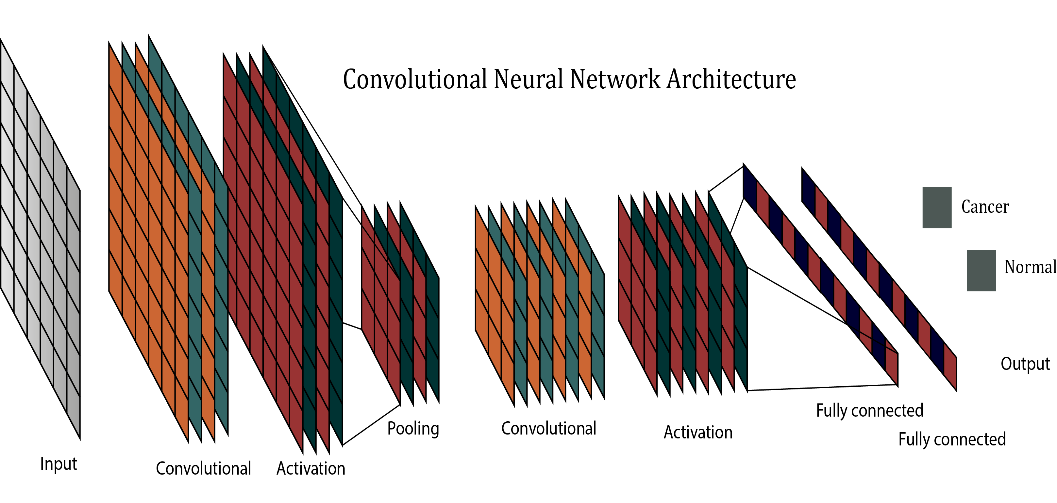
\includegraphics[width=14cm]{chaps/lr/cnn_arch}}
	\caption{معماری یک شبکه عصبی کانولوشنی}
	\label{fig:ch_lr:cnn_arch}
\end{figure}

همانطور که قبلاً بیان شد، \glspl{convnet} مدل‌های \gls{fullyconnectedffnn} هستند که از لایه‌های زیادی تشکیل شده اند. بسیاری از این مدل‌ها محدودیت‌های پارامتر و مکانی دارند که در ادامه توضیح داده خواهد شد. با این حال، آنها در تغییراتی که بر ورودی‌شان اعمال می‌کنند تفاوت دارند. در اینجا ما تمام لایه‌های یک شبکه کانولوشنی و توابع مورد استفاده در آموزش آن‌ها را شرح می‌دهیم. یک معماری می‌تواند یاد بگیرد که مسائل بسیار متفاوتی را حل کند تا زمانی که پارامترها برای هر یک از مسائل به خوبی بهینه شوند.

لایه ورودی فقط نمایشی از داده خام است که به مدل داده می‌شود که نیاز به شکل ورودی ثابت دارد. در رایج ترین حالت، یک تصویر به یک آرایه 3 \gls{dimension}ی تبدیل می‌شود با ابعاد [$w, h,3$] که $w$ و $h$ عرض و ارتفاع هستند. \gls{dimension} آخر به دلیل استفاده از تصاویر رنگی \lr{RGB\LTRfootnote{Red Green Blue}} اغلب $3$ است. وقتی از تصاویر \gls{xray} استفاده می‌کنیم چون دارای یک \gls{channel} \gls{intensity} هستند \gls{dimension} سوم برابر با $1$ است.

این لایه اصلی ترین لایه شبکه‌های عصبی کانولوشنی است و این شبکه‌ها نام‌ خود را از این لایه‌ها دریافت می‌کنند. وظیفه این لایه استخراج ویژگی‌ها است. این لایه عملیات کانولوشن را بر روی داده ورودی اعمال می‌کند و خروجی‌هایی به نام \gls{featuremap} از این لایه به دست می‌آید. در نتیجه تمامی نورون‌ها در یک \gls{featuremap}، وزن‌ها و \glspl{bias} مشابه و مشترکی دارند که باعث می‌شود، ویژگی‌های تصویر در موقعیت‌های مختلف قابل شناسایی باشند. از طرف دیگر این اشتراک وزن‌ها باعث کاهش تعداد پارامتر‌های مورد نیاز برای آموزش می‌شود. در شبکه‌های کانولوشن اتصالات به صورت نواحی کوچک و محلی صورت می‌گیرد. به بیان دیگر هر نورون در نخستین لایه مخفی به ناحیه کوچکی از نورون‌های ورودی متصل می‌شود. برای مثال اگر این ناحیه $5\times 5$ باشد این ناحیه کوچک $25$ پیکسلی \gls{localreceptivefield}  یا \gls{kernel} کانولوشن نامیده می‌شود. با توجه به شکل \ref{fig:ch_lr:cnn_conv5} یک تصویر ورودی $28\times 28$ داریم که یک \gls{kernel} $5\times 5$ بر روی پیکسل‌های ورودی از چپ به راست حرکت می‌کند هر پنجره به نورونی در لایه مخفی متصل می‌شود. بناباین همان طور که در شکل \ref{fig:ch_lr:cnn_conv5} مشخص است لایه مخفی شامل یک شبکه $24\times 24$ نورونی خواهد بود.

\begin{figure}[!ht]
	\centerline{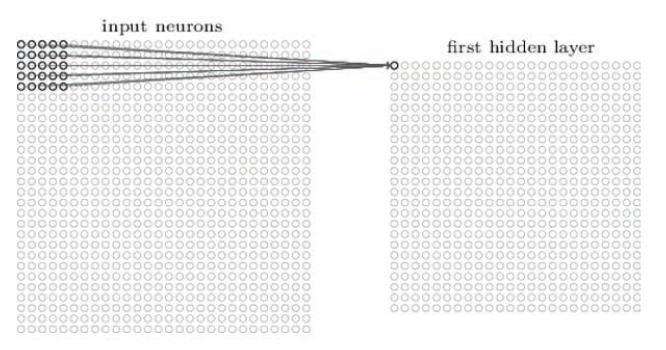
\includegraphics[width=11cm]{chaps/lr/cnn_conv5}}
	\caption{
		عملیات \gls{convolution} در یک \gls{convnet} با \gls{kernel} $5\times 5$
	}
	\label{fig:ch_lr:cnn_conv5}
\end{figure}

در شکل \ref{fig:ch_lr:cnn_conv5} هر نورون لایه مخفی دارای یک \gls{bias} و تعداد $5\times 5$ وزن می‌باشد که به  ناحیه ادراکی خود متصل شده است. تمامی نورون‌های لایه مخفی مذکور که دارای ابعاد $24\times 24$ هستند، دارای وزن‌ها و \glspl{bias}ی مشترکی می‌باشند. به عبارت دیگر خروجی نورون لایه کانولوشن $y_{w,h,m}$ در طول و عرض $w,h$ و عمق $m$ به صورت رابطه \ref{eq:ch_lr:neuron_ouput} است.
\begin{equation}
	y_{w,h,m} = f\left(\sum_{i=(w-1)S+1}^{(w-1)S+K} \sum_{j=(h-1)S+1}^{(h-1)S+K} \sum_{k=1}^{N} W_{k,m}(x_{i,j,k})+b_m\right)
	\label{eq:ch_lr:neuron_ouput}
%	\caption{خروجی نورون لایه کانولوشن}
\end{equation}

که در این رابطه $f$ \gls{activationfunction}، $b_m$ بایاس مشترک نورون‌ها، $W_{k,m}$ وز‌ن‌های $5\times 5$ مشترک نورون‌ها و $x_{i,j,k}$ ورودی در موقعیت $i,j,k$ می‌باشد. بنابراین تمامی نورون‌های واقع در لایه مخفی اول به طور دقیق ویژگی‌های مشابهی را در نواحی مختلف تصویر شناسایی می‌کنند. در نهایت خروجی لایه ورودی یا نورون‌های لایه مخفی به عنوان \gls{featuremap} شناخته می‌شوند. ابعاد مربوط به ماتریس خروجی لایه کانولوشن $W_2\times H_2 \times D_2$ که از ماتریس ورودی با ابعاد $W_1\times H_1 \times D_1$ است، به صورت رابطه \ref{eq:ch_lr:conv_ouput} به دست می‌آید.

\begin{equation}
	W_2 = \frac{W_1-F+2P}{S+1}, \qquad H_2=\frac{H_1-F+2P}{S+1}, \qquad D_2=K
	\label{eq:ch_lr:conv_ouput}
\end{equation}
در روابط \ref{eq:ch_lr:conv_ouput} که بیانگر نحوه محاسبه ابعاد ماتریس خروجی کانولوشن است،
$F, P, S$ و $k$
به ترتیب نشان دهنده اندازه \gls{kernel}، مدار \gls{zeropadding}، اندازه \gls{stride} و تعداد فیلترها می‌باشد. طبق این روابط به ازای هر فیلتر تعداد $F\times F\times D_1$ وزن داریم و با توجه به تعداد $k$ فیلتر موجود، در مجموع تعداد $k(F\times F\times D_1)$ وزن و $k$ بایاس ایجاد می‌شود. بنابراین تعداد پارامترهایی که شبکه در یک لایه کانولوشن خود می‌بایست آموزش ببیند زیاد است.

بکارگیری \gls{activationfunction} در لایه کانولوشن باعث ایجاد خصوصیات غیر خطی در خروجی می‌شود و باعث می‌شود عملکرد مدل متمایز کننده‌تر شود. این توابع با حفظ اندازه لایه، بدون نیاز به پارامترهای آموخته شده، یک عملكرد ساده عنصرگونه در مدل انجام می‌دهند. تابع \gls{relu} متداول ترین تابع مورد استفاده به خاطر آسان کردن مرحله آموزش است. مثال‌های دیگر شامل تابع \gls{sigmoid} و \gls{hyperbolictangent} است.
\begin{equation}
	\begin{aligned}
		\text{ReLU:}&\quad r_{m,n,c} = \max\{0,l_{x,y,z}\} \\
		\text{Sigmoid:}&\quad s_{m,n,c} = \frac{1}{1-\exp(-l_{x,y,z})}
	\end{aligned}
	\label{eq:ch_lr:relu-sigmoid}
\end{equation}
\begin{figure}[!ht]
	\centerline{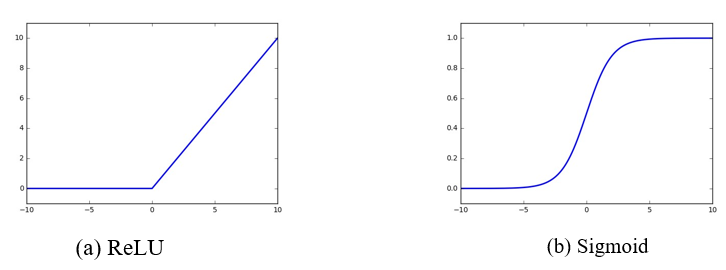
\includegraphics[width=14cm]{chaps/lr/activation_functions}}
	\caption{(\lr{a}) \gls{activationfunction} \lr{ReLU} و (\lr{b}) \gls{activationfunction} \gls{sigmoid}	
	}
	\label{fig:ch_lr:activation_functions}
\end{figure}
در یک شبکه عصبی کانولوشن معمولا پس از هر لایه کانولوشن یک لایه \lr{pooling} قرار می‌گیرد . این لایه‌ از آن جهت اهمیت دارد که باعث کاهش تعداد پارامترهایی می‌شود که باید آموزش ببینند. بنابراین با بکارگیری این لایه ضمن کاهش محاسبات مورد نیاز در بخش آموزش، باعث کنترل \gls{overfitting} احتمالی در شبکه می‌شود. این لایه بر روی هر عمق از ورودی اعمال می‌شود و اندازه آن را تغییر می‌دهد. دو تابع عملکردی معروف این لایه \lr{max-pooling} و \lr{mean-pooling} نام دارند که تابع اول دارای کاربرد بیشتری در \glspl{convnet} است. طریقه عملکرد \lr{max-pooling} به این صورت است که در هر پنجره بزرگترین \gls{pixel} را به خروجی می‌فرستد. این پنجره بر روی تصویر مانند تابع کانولوشن از چپ به راست و از بالا به پایین با انداه گام‌های مشخص حرکت می‌کند و نتیجه را به خروجی می‌فرستد. به دلیل اینکه این عملیات بر روی تمامی عمق‌ها اعمال می‌گردد، عمق خروجی همان عمق ورودی به لایه \lr{pooling} است. یک مثال از عمل \lr{max-pooling} در شکل \ref{fig:ch_lr:max_pooling} به نمایش گذاشته شده است.
\begin{equation}
	\text{with}\ l \in [s\times x, s\times x + m], j\in [s\times y, s\times y + m], \quad R_{x,y,x} = \max \{l_{i,j,z}\}
	\label{eq:ch_lr:max-pooling}
\end{equation}
\begin{figure}[!ht]
	\centerline{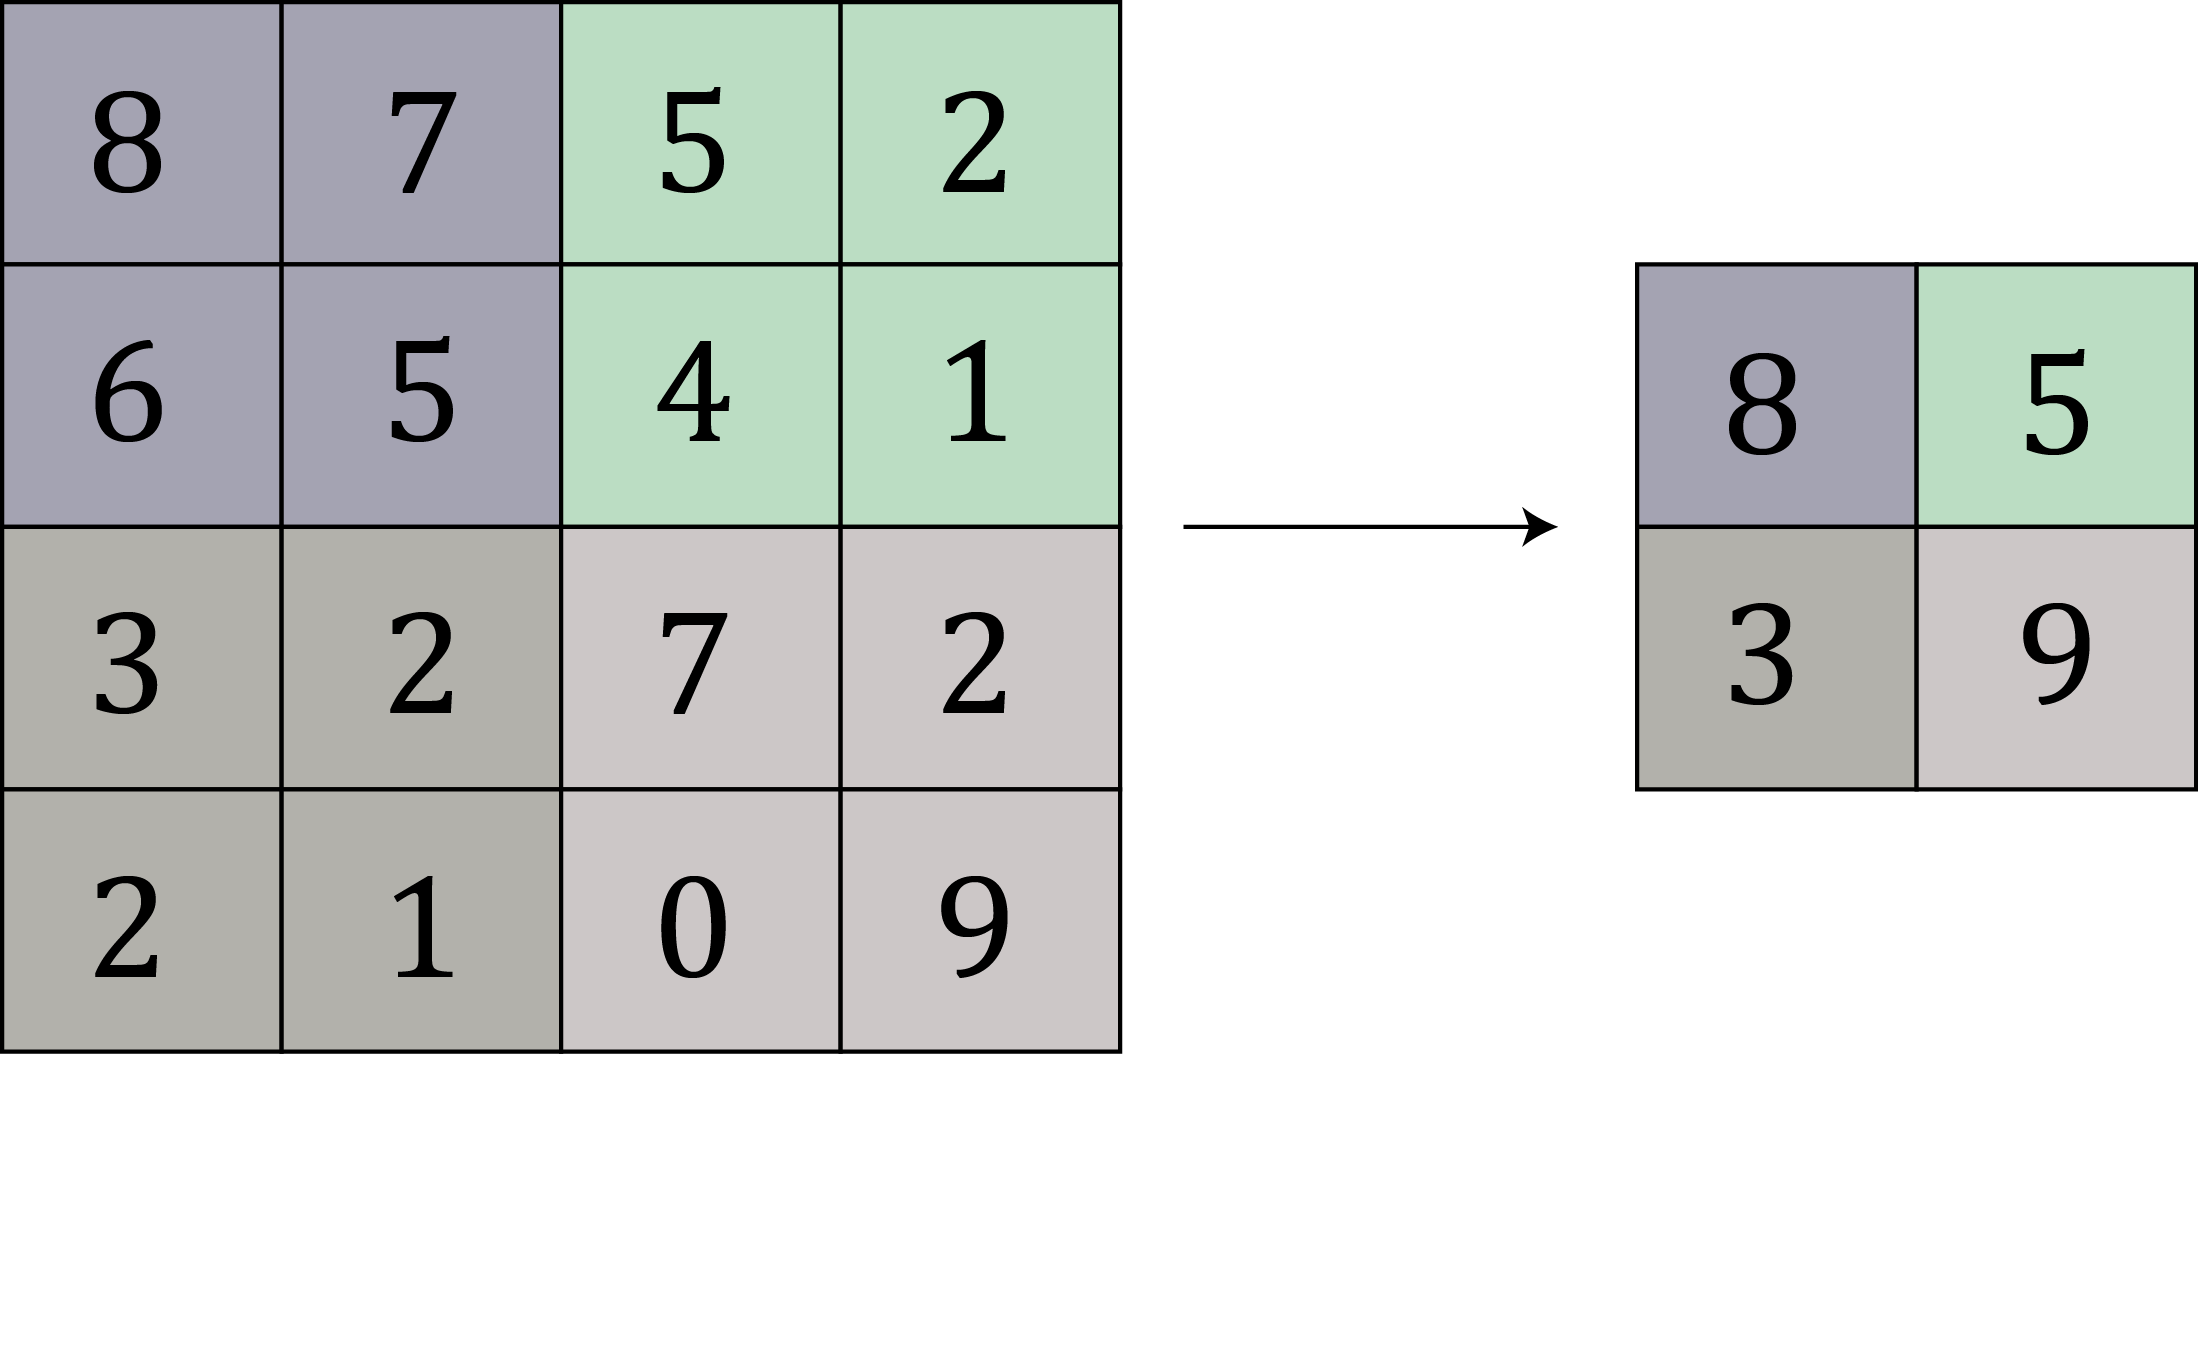
\includegraphics[width=8cm]{chaps/lr/max_pooling}}
	\caption{
		تابع \lr{max-pooling} بر روی آرایه دو بعدی کوچک $m=2$ و $s=2$
	}
	\label{fig:ch_lr:max_pooling}
\end{figure}
لایه کاملا متصل لایه آخر یک شبکه عصبی کانولوشنی محسوب می‌شود و اتصالات کاملی با خروجی لایه قبلی ایجاد می-کند. این لایه ورودی را دریافت و سپس خروجی را به صورت برداری با $N$ مولفه تولید می‌کند که $N$ تعداد کلاس‌هایی که شبکه باید طبقه بندی کند است. در واقع یک شبکه  \gls{convnet} جهت تولید یک بردار خروجی با $N$ مولفه عددی طراحی می‌شود که هر عدد در این بردار خروجی درصد احتمال تعلق به کلاس مورد نظر را نشان می‌دهد. برای یک مسئله با تعداد $k$  کلاس، $k$ نورون خروجی داریم که هر احتمال را با تابع \lr{SoftMax} محاسبه می‌کنند
\begin{equation}
	P(C)_j = \frac{e^{c_j}}{\sum^{K}_{k=1}e^{c_k}}
	\label{eq:ch_lr:softmax}
%	\caption{محاسبه احتمال هر کلاس با تابع \lr{SoftMax}}
\end{equation}
اگر دو کلاس داشته باشیم می‌توانیم از تابع \lr{SoftMax} با دو خروجی استفاده کنیم یا از یک نورون استفاده کنیم و تابع \gls{sigmoid} را محاسبه کنیم. برای دو کلاس احتمال توسط معادله \ref{binary_softmax} محاسبه می‌شود
\begin{equation}
	P(1) = \frac{1}{1+e^i} \qquad \qquad P(0) = 1-P(1)
	\label{eq:ch_lr:binary_softmax}
	%	\caption{احتمال کلاس1 و احتمال کلاس0}
\end{equation}
\gls{dropout} یک روش بسیار رایج برای جلوگیری از \gls{overfitting} شبکه عصبی مصنوعی از جمله مدل‌های \gls{deeplearning} است\cite{srivastava2014dropout}.
ایده این تکنیک این است که با جلوگیری از هماهنگی نورون‌ها ، ویژگی‌های قوی تری ایجاد شود. اجرای آن ساده است تنها نیاز به بهم چسباندن لایه‌های اضافی در شبکه معمولا پس از توابع فعال سازی است. این ماژول بطور تصادفی برخی از نقاط نقشه ویژگی ورودی را  صفر می‌کند. هریک از ماژول‌ها دارای یک احتمال مستقل $\sigma$ برای نگهداری نقاط هستند و در صورت بروز چنین اتفاقی ، توسط  $\frac{1}{\sigma}$ مقیاس بندی می‌شوند. نقاطی که نگهداری نمی‌شوند بر روی صفر تنظیم می‌شوند. این لایه فقط یک پارامتر $\sigma$ دارد، که برای آموزش در فاصله $[0,1]$ قرار دارد و برای آزمایش روی $1$ قرار می‌گیرد. به طور شهودی، می‌توان این فرآیند را به عنوان حذف برخی از نورون‌های شبکه عصبی ، به طور موقت ، همراه با اتصالات ورودی و خروجی آن تصور کرد. مکانیزم حذف، نورون‌هایی را که به اتصالات ورودی کمتری متکی هستند را در نظرمی‌گیرد. زیرا افت یک زیر مجموعه از ورودی‌ها در مقایسه با یک نورون که به بسیاری از ورودی‌ها متکی است، قابل توجه‌تر خواهد بود و به این ترتیب ویژگی‌های کلی‌تر مهم‌تر می‌شوند. شکل \ref{fig:ch_lr:dropout} یک مثال از لایه \gls{dropout} را نمایش می‌دهد.
\begin{figure}[!ht]
	\centerline{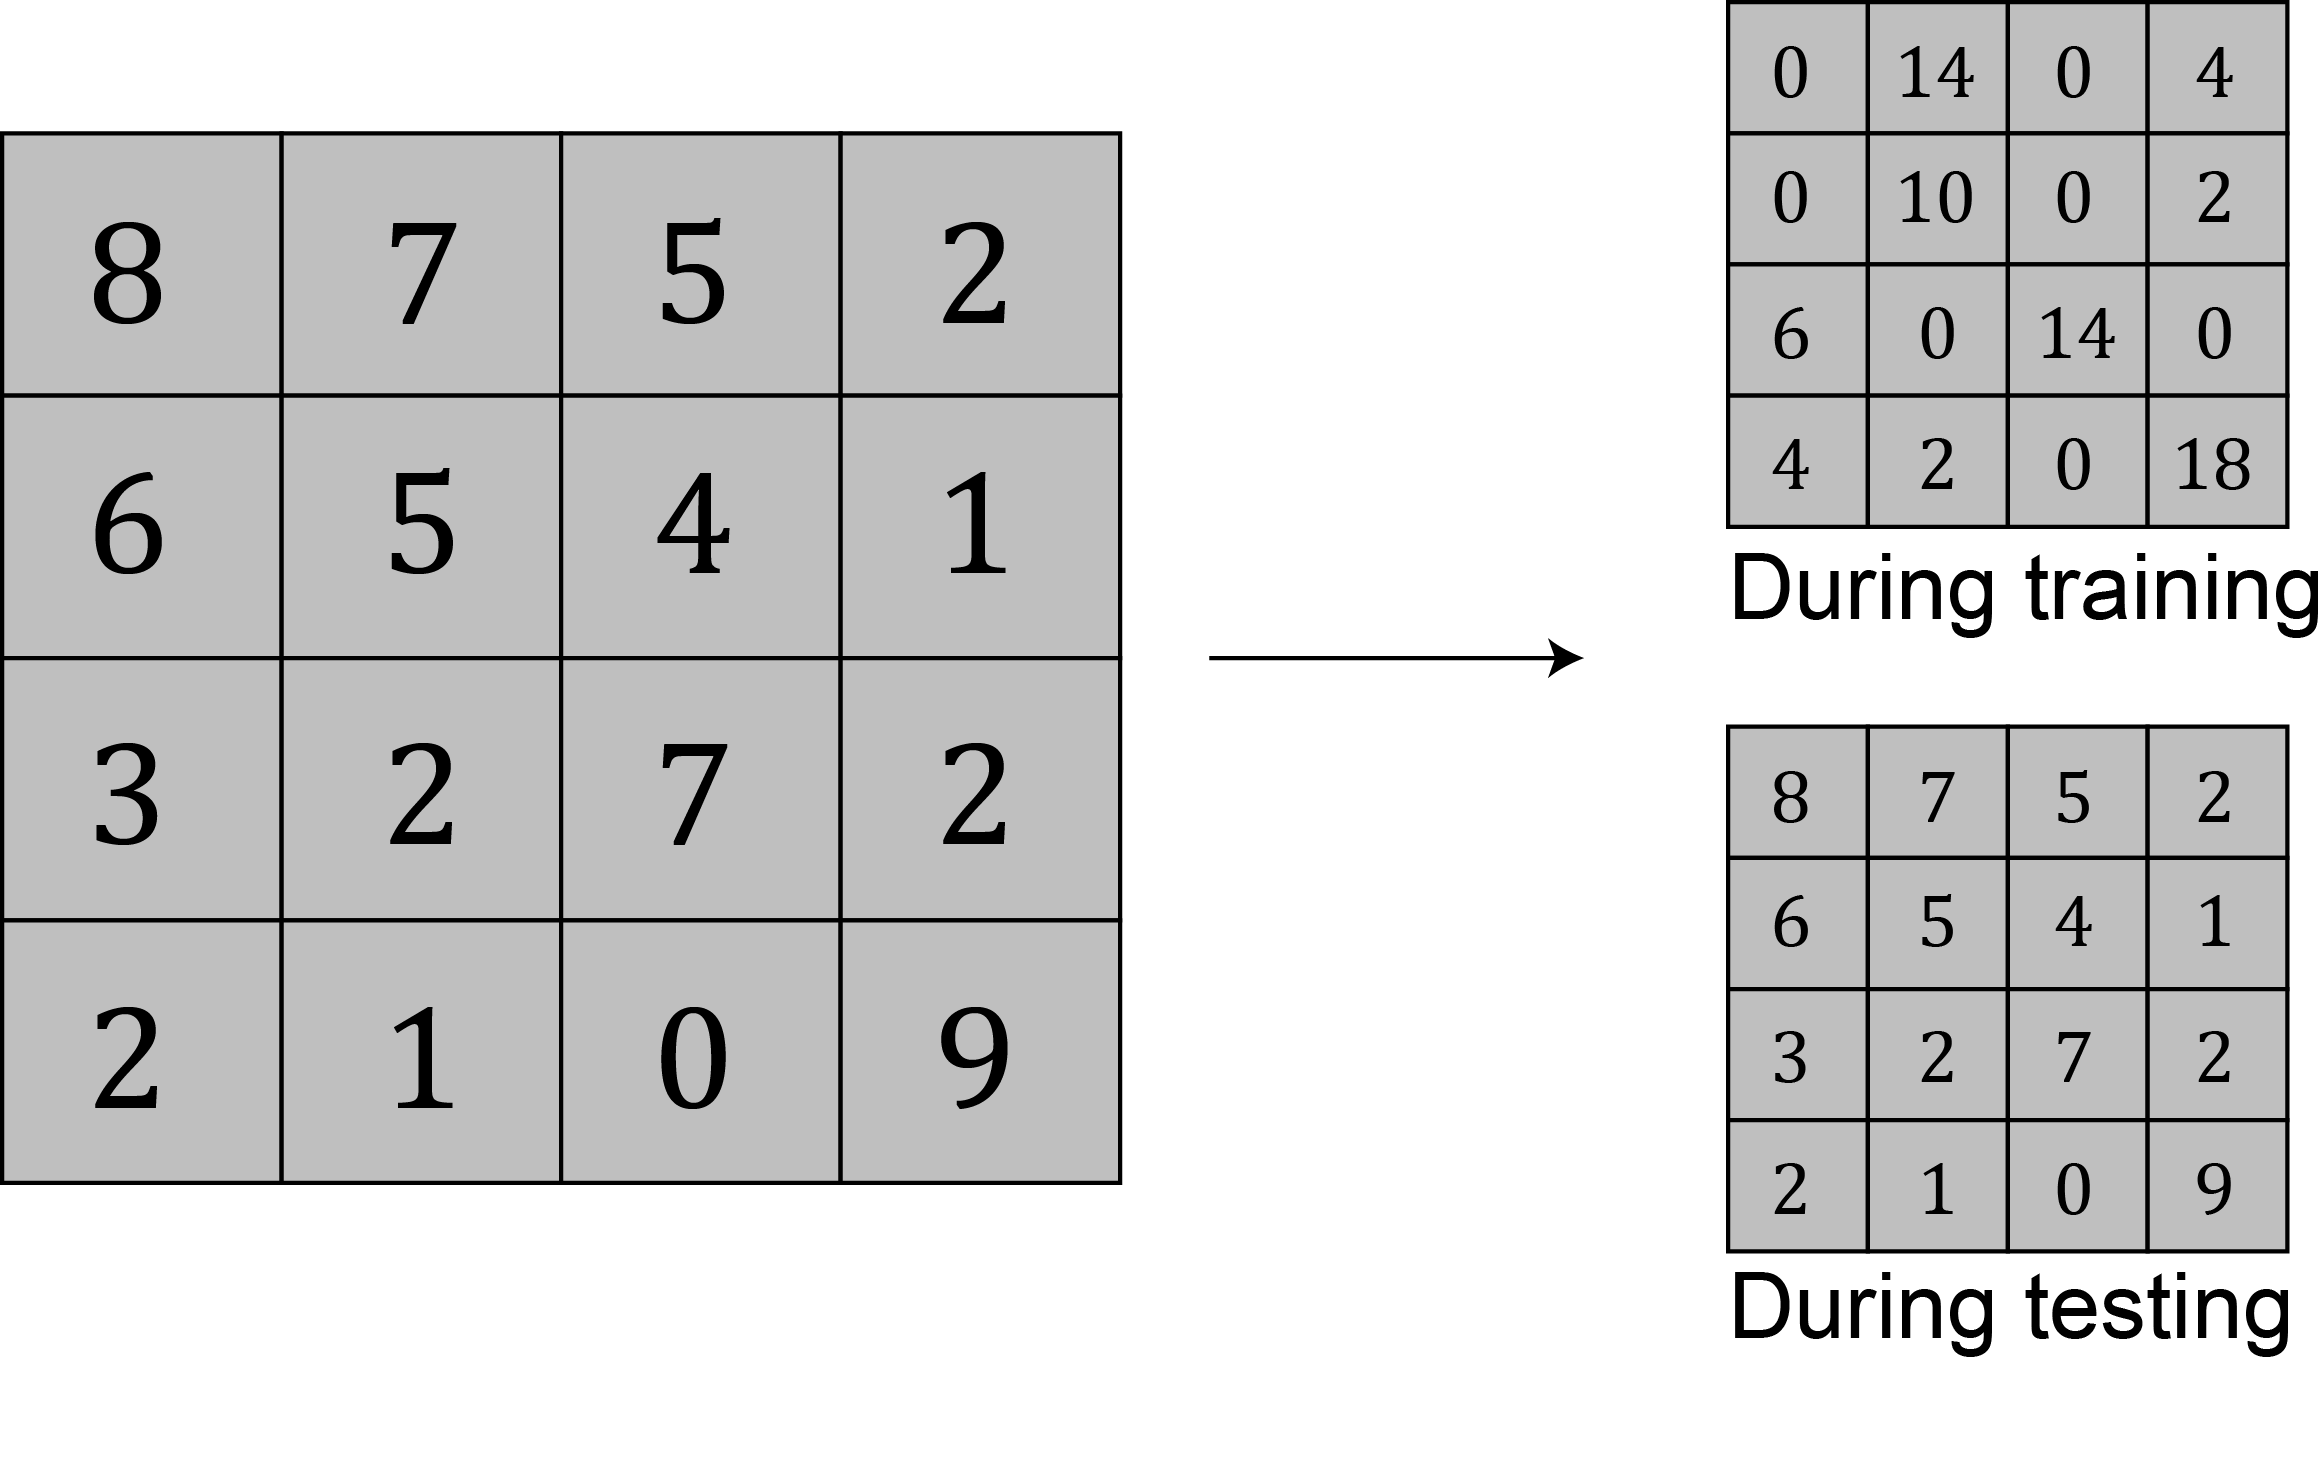
\includegraphics[width=10cm]{chaps/lr/dropout}}
	\caption{
	لایه \gls{dropout} با $\sigma=0.5$
	}
	\label{fig:ch_lr:dropout}
\end{figure}
\gls{batchnormalization} یک تکنیک جدید ولی خیلی کارامد است. در طی آموزش مدل‌های عمیق ، وزن‌ها در هر \gls{iteration}  به روز می‌شوند.
یک اثر جانبی این امر این است که در هر لایه توزیع‌های ورودی تغییر می‌کند، پدیده ای که به آن  \gls{internalcovariateshift}می‌گویند. این پدیده فرایند آموزش را کند می‌کند، به مقدار دهی دقیق‌تر وزن احتیاج دارد و مانع \gls{optimization} مدل‌های غیرخطی اشباع، مانند مماس‌های \gls{sigmoid} یا هایپربولیک می‌شود. برای حل این مشکل \gls{batchnormalization} را پیشنهاد می‌شود که مشابه با \gls{dropout}، به عنوان لایه ای در شبکه با رفتارهای متفاوت در حین آموزش و آزمون پیاده سازی می‌شود. برای رفع مشکل تغییر \gls{covariance} داخلی ، این لایه برای هر دسته آموزش  با کم کردن میانگین و تقسیم بر \gls{standarddeviation} همه نورون‌های عمق مشابه، ورودی خود را نرمال می‌کند. به میانگین و \gls{standarddeviation} آمار \lr{mini-batch}  گفته می‌شود. برای اطمینان از اینكه مدل می‌تواند دقیقاً همان تابع را با یا بدون \gls{batchnormalization} عادی نشان دهد ، دو وزن جدید قابل تمرین $\gamma$ و $\beta$ اضافه می‌شوند كه خروجی را اندازه گیری و جبران می‌كنند. بنابراین خروجی به صورت معادله \ref{eq:ch_lr:batch_normalization} است.
\begin{equation}
	\begin{aligned}
		\text{در طی آموزش}&: \quad I_c = \gamma \left(\frac{I_c-\text{\lr{mean}}(I_c)}{\text{\lr{std}}(I_c)}\right)+\beta  
		\\
		\text{در طی آزمایش}&: \quad I_c = \gamma \left(\frac{I_c-u_c}{v_c}\right)+\beta  
	\end{aligned}
	\label{eq:ch_lr:batch_normalization}
	%	\caption{احتمال کلاس1 و احتمال کلاس0}
\end{equation}
که $u_c$ و $v_c$ متوسط‌های در حال اجرا $\text{\lr{mean}}(I_c)$ و $\text{\lr{std}}(I_c)$ هستند. نشان داده شده است که \gls{batchnormalization} باعث آهنگ یادگیری بالاتر می‌شود و مدل در تکرارهای کمتری همگرا خواهد شد. این روش دارای اثر \gls{regularization} است. 
مدل با استفاده از \gls{costfunction} یاد می‌گیرد. این روشی است برای ارزیابی اینکه تا چه میزان خوب یک الگوریتم داده‌های مشاهده شده را می‌تواند مدل سازی کند. اگر پیش بینی‌ها بیش از حد از نتایج واقعی منحرف شوند ، \gls{costfunction} مقدار بالایی خواهد داشت. به تدریج، با کمک برخی توابع بهینه سازی، تابع هزینه می‌آموزد تا خطا در پیش بینی را کاهش دهد.

بهینه سازی مهمترین بخش در الگوریتم‌های یادگیری عمیق است. این کار با تعریف \gls{costfunction} شروع می‌شود و با به حداقل رساندن آن با استفاده از یک روش بهینه سازی به پایان می‌رسد. فرض کنید یک مجموعه داده $D$ با تعداد $I$ تصویر داریم. این تصاویر می‌توانند ضایعه باشند یا نباشند، بنابراین دارای برچسب $y\in \{0,1\}$ هستند.

باید مدلی بسازیم که با توجه به یک تصویر ورودی $I_i$، یک احتمال $p(I_i)$ تولید کند که تا حد ممکن به برچسب مربوط به آن تصویر ($y_i$) نزدیک باشد. برای این منظور الگوریتم‌های بهینه سازی متفاوتی وجو دارد مانند \lr{Adam}، \lr{SGD}\LTRfootnote{Stochastic gradient descent} و 
\lr{Adadelta}.\\
 به حداقل رساندن \gls{costfunction} با کاهش گرادیان تقریباً رایج ترین الگوریتم برای بهینه سازی شبکه‌‌های عصبی است. اگر \gls{costfunction} \gls{binarycrossentropy} باشد و بخواهیم محاسبه کنیم که $p(I_i)$ تا چه حد خوب می‌تواند برچسب $y_i$ را تقریب بزند از معادله \ref{eq:ch_lr:binary_ce} استفاده می‌شود.
 \begin{equation}
 	L = \frac{1}{|\mathcal{D}|}  \sum_i^{|\mathcal{D}|}\Big(y_i \log\big(P(I_i)\big) + (1-y_i) \log\big(1-P(I_i)\big)\Big)
 	\label{eq:ch_lr:binary_ce}
 	%	\caption{تابع خطا cross-entropy binary}
 \end{equation}
 احتمال برای یک ورودی به وزن‌های آن ($\theta$) بستگی دارد و با
 $p(I, \theta)$ 
 نمایش داده می‌شود. با توجه به $\theta$ می‌توان $L(\theta)$ را با اجرای مدل بر روی مجموعه داده به دست آورد.
 
 \gls{backpropagation}
 اساس آموزش شبکه عصبی است. این عمل تنظیم-دقیق  وزن‌های یک شبکه عصبی بر اساس میزان \gls{loss} در هر \gls{epoch} قبلی است که این امر با محاسبه مشتق‌های تابع خطا بر اساس وزن‌ها 
 $\nabla_\theta L(\theta)$
 در زمان آموزش امکان پذیراست. تنظیم مناسب وزن‌ها  باعث کاهش میزان خطا می‌شود. در فرایند \gls{backpropagation}  ابتدا ورودی در سراسر شبکه انتشار داده می‌شود سپس $L(\theta)$ محاسبه شده و در نهایت این \gls{loss} از طریق تمام وزن‌ها در شبکه رو به عقب منتشر می‌شود. مشتق \gls{costfunction} از خروجی توسط معادله \ref{eq:ch_lr:dif_cf} محاسبه می‌شود.
 \begin{equation}
 	\frac{\partial L}{\partial P} = \frac{\partial \Big(-\big(y_i \log(p) + (1-y)\log(1-P)\big)\Big)}{\partial P} = \frac{P-y}{P(1-P)}
 	\label{eq:ch_lr:dif_cf}
 	%	\caption{محاسبه مشتق از تابع هزینه}
 \end{equation}
 همچنین محاسبه مشتق \gls{costfunction} $L$ از ورودی $i$ به صورت معادله \ref{eq:ch_lr:dif_cf_i} محاسبه می‌شود.
  \begin{equation}
 	\frac{\partial L}{\partial i} = \frac{\partial L}{\partial P} \frac{\partial P}{\partial i} = P-y
 	\label{eq:ch_lr:dif_cf_i}
 \end{equation}
 همچنین محاسبه مشتق \gls{costfunction} بر اساس وزن‌های لایه آخر $w$ به صورت، 
   \begin{equation}
 	\frac{\partial L}{\partial w} = \frac{\partial L}{\partial P} \frac{\partial P}{\partial i}  \frac{\partial i}{\partial w}= (P-y)a
 	\label{eq:ch_lr:dif_cf_w}
 \end{equation}
 می‌باشد که $a$ در آن برابر با ترکیب خطی از ورودی‌های لایه آخر است. این کار را می‌توان به راحتی به لایه‌های قبلی تعمیم داد، بنابراین می‌توان $\nabla _\theta L(\theta)$ را محاسبه کرد.
 \section{شبکه‌های عصبی بازگشتی}
 قبل از آشنا شدن با \glspl{rnn} بهتر است مروری بر مفهوم شبکه عصبی داشته باشیم. شبکه‌های عصبی مجموعه‌ای از الگوریتم‌ها هستند که شباهت نزدیکی به مغز انسان داشته و به منظور تشخیص الگوها طراحی شده‌اند. شبکه‌ی عصبی داده‌های حسی را از طریق ادراک ماشینی ، برچسب زدن یا خوشه بندی ورودی‌های خام تفسیر می‌کند. شبکه می‌تواند الگوهای عددی را شناسایی ‌کند؛ این الگوها بردارهایی هستند که همه‌ی داده‌های دنیای واقعی (تصویر، صدا، متن یا سری‌های زمانی) برای تفسیر باید به شکل آن‌ها درآیند. شبکه‌های عصبی مصنوعی از تعداد زیادی مؤلفه‌ی پردازشی (نورون) تشکیل شده‌اند که اتصالات زیادی بینشان وجود دارد و برای حل یک مسئله با یکدیگر همکاری دارند.
 شبکه‌ی عصبی مصنوعی معمولاً تعداد زیادی پردازشگر دارد که به صورت موازی کار می‌کنند و در ردیف‌هایی کنار هم قرار می‌گیرند. ردیف اول، همچون عصب‌های بینایی انسان در پردازش بصری، اطلاعات ورودی‌های خام را دریافت می‌کند. سپس هر کدام از ردیف‌های بعدی، به جای ورودی خام، خروجی ردیف قبلی را دریافت می‌کنند؛ در پردازش بصری نیز نورون‌هایی که از عصب بینایی فاصله دارند، سیگنال را از نورون‌های نزدیک‌تر می‌گیرند. ردیف آخر خروجی کل سیستم را تولید می‌کند.

\subsection{شبکه عصبی بازگشتی چیست؟}
 شبکه‌ی عصبی بازگشتی شکلی از شبکه‌ی عصبی پیشخور است که یک حافظه‌ی داخلی دارد. شبکه عصبی بازگشتی ذاتاً بازگشتی است، زیرا یک تابع یکسان را برای همه‌ی داده‌های ورودی اجرا می‌کند، اما خروجی داده‌ی (ورودی) فعلی به محاسبات ورودی قبلی بستگی دارد. خروجی بعد از تولید، کپی شده و مجدداً به شبکه‌ی بازگشتی فرستاده می‌شود. این شبکه برای تصمیم‌گیری، هم ورودی فعلی و هم خروجی که از ورودی قبلی آموخته شده را در نظر می‌گیرد.
 شبکه عصبی بازگشتی برخلاف شبکه‌های عصبی پیشخور می‌توانند از حالت (حافظه‌ی) درونی خود برای پردازش دنباله‌هایی از ورودی‌ها استفاده کنند. این خاصیت باعث می‌شود در مسائلی همچون تشخیص دست‌خط زنجیره‌ای یا تشخیص گفتار کاربرد داشته باشند. در سایر شبکه‌های عصبی، ورودی‌ها از یکدیگر مستقل هستند، اما در شبکه عصبی بازگشتی ورودی‌ها به هم مرتبط می‌باشند. به شکل \ref{fig:ch_lr:rnn} توجه کنید،
 \begin{figure}[!ht]
 	\centerline{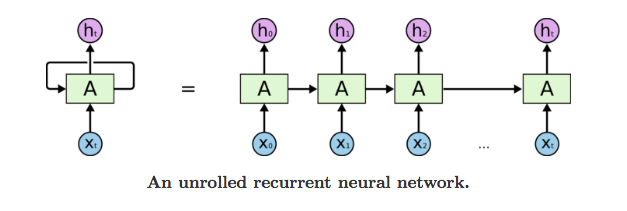
\includegraphics[width=14cm]{chaps/lr/rnn}}
 	\caption{
 		یک نمونه بازشده \gls{rnn}
 	}
 	\label{fig:ch_lr:rnn}
 \end{figure}
 این شبکه ابتدا $X_0$ را از دنباله‌ی ورودی‌ها گرفته و خروجی $h_0$ را تولید می‌کند که همراه با $X_1$ ورودی گام بعدی محسوب خواهند شد. یعنی $h_0$ و $X_1$ ورودی گام بعدی هستند. به همین صورت $h_1$ بعدی همراه با $X_1$ ورودی گام بعدی خواهند بود. شبکه عصبی بازگشتی بدین طریق می‌تواند هنگام آموزش زمینه را به خاطر داشته باشد.
 فرمول \gls{state} کنونی به صورت رابطه \ref{eq:ch_lr:rnn_cs} خواهد بود که در آن،
 \begin{equation}
 	h_t = f(h_{t-1}, x_t)
 	\label{eq:ch_lr:rnn_cs}
 \end{equation}
 خواهد بود که در آن $h_t$ برابر است با،
 \begin{equation}
 	h_t = \tanh(W_{hh}h_{t-1} + W_{hx}x_t)
 	\label{eq:ch_lr:rnn_ht}
 \end{equation}
 در این فرمول $W$ وزن، $h$ تک‌بردار نهان، $W_hh$ وزن حالت نهان قبلی، $W_{hx}$ وزن حالت ورودی کنونی و $\tanh$ \gls{activationfunction} است که با استفاده از تابعی غیرخطی، خروجی را فشرده می‌کند تا در بازه‌ی $[1, -1]$ جای گیرند. در نهایت \gls{state} خروجی $Y_t$ از طریق رابطه \ref{eq:ch_lr:rnn_hy} بدست می‌آید،
 \begin{equation}
 	y_t = W_{hy}h_t
 	\label{eq:ch_lr:rnn_hy}
 \end{equation}
 که در آن $W_{hy}$ برابر وزن در \gls{state} تولید شده را نشان می‌دهد.
 
 \subsection{مزایای \gls{rnn}}
 شبکه عصبی بازگشتی می‌تواند دنباله‌ای از داده‌ها را به شکلی مدل‌سازی کند که هر نمونه وابسته به نمونه‌های قبلی به نظر برسد. شبکه عصبی بازگشتی را می‌توان با لایه‌های پیچشی نیز به کار برد تا گستره‌ی همسایگی پیکسلی را افزایش داد.
 
 \subsection{معایب \gls{rnn}}
 \begin{itemize}
 	\item گرادیان کاهشی و مشکلات ناشی از آن
 	\item آموزش بسیار دشوار
 	\item ناتوانی در پردازش دنباله‌های طولانی از ورودی در صورت استفاده از \gls{activationfunction}  $\tanh$ یا \lr{ReLU}
 \end{itemize}

\subsection{کاربردهای \gls{rnn}}
\begin{itemize}
	\item شرح نویسی عکس\LTRfootnote{Image Captioning}: شبکه عصبی بازگشتی با تحلیل حالت کنونی عکس، برای شرح نویسی عکس به کار می‌رود
	\item پیش بینی سری‌های زمانی\LTRfootnote{Time Series Prediction}: هر مسئله سری زمانی مانند پیش بینی قیمت یک سهام در یک ماه خاص، با \gls{rnn} قابل انجام است
	\item
	پردازش زبان طبیعی\LTRfootnote{Natural Language Processing}: کاوش متن و تحلیل احساسات می‌تواند با استفاده از \gls{rnn} انجام شود
	\item
	ترجمه ماشینی\LTRfootnote{Machine Translation}: شبکه \gls{rnn} می‌تواند ورودی خود را از یک زبان دریافت و آن را به عنوان خروجی به زبان دیگری ترجمه کند
\end{itemize}
 
\subsection{انواع \gls{rnn}}
\noindent
 به طور کلی 4 نوع شبکه عصبی بازگشتی داریم:\\
 یک به یک (\lr{one to one}) : این نوع شبکه عصبی به عنوان شبکه عصبی وانیلی نیز شناخته می‌شود و برای مسائل یادگیری ماشین که یک ورودی و یک خروجی دارند به کار می‌رود.

 \begin{figure}[!ht]
 	\centering
 	\subfloat[یک به یک]{
 		\centering
 		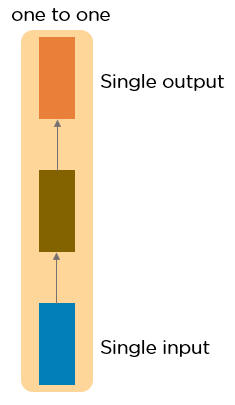
\includegraphics[width=0.17\textwidth]{chaps/lr/rnn_oto}
 		\label{fig:ch_lr:rnn_oto}
 	}
 	\hfill
 	\subfloat[یک به چند]{
 		\centering
 		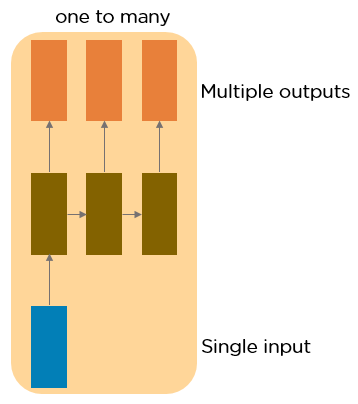
\includegraphics[width=0.26\textwidth]{chaps/lr/rnn_otm}
 		\label{fig:ch_lr:rnn_otm}
 	}
 	\hfil
 	\subfloat[چند به یک]{
 		\centering
 		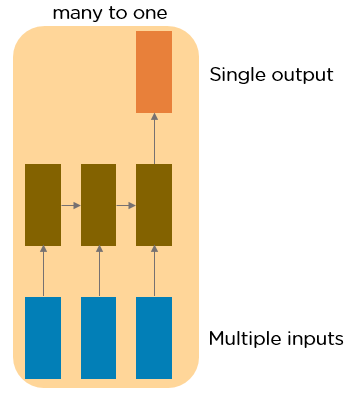
\includegraphics[width=0.26\textwidth]{chaps/lr/rnn_mto}
 		\label{fig:ch_lr:rnn_mto}
 	} 	\hfill
 	\subfloat[چند به چند]{
 		\centering
 		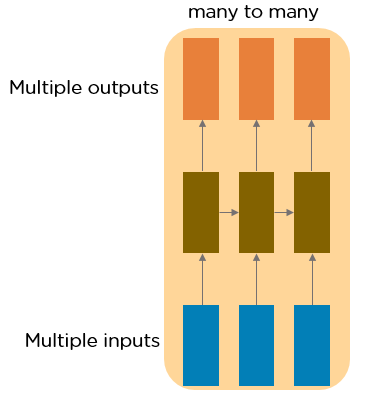
\includegraphics[width=0.26\textwidth]{chaps/lr/rnn_mtm}
 		\label{fig:ch_lr:rnn_mtm}
 	}
 	\caption{ساختار \gls{rnn}}
 	\label{fig:ch_lr:rnn_xtx}
 \end{figure}
 
% 
% \begin{figure}[!ht]
% 	\centerline{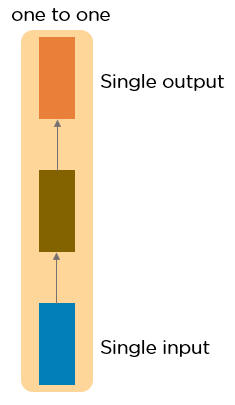
\includegraphics[width=4cm]{chaps/lr/rnn_oto}}
% 	\caption{ساختار \gls{rnn} یک به یک}
% 	\label{fig:ch_lr:rnn_oto}
% \end{figure}
%\\
 یک به چند (\lr{one to many}): این شبکه عصبی بازگشتی دارای یک ورودی و چند خروجی است. یک نمونه آن، شرح نویسی عکس است.
% \begin{figure}[!ht]
% 	\centerline{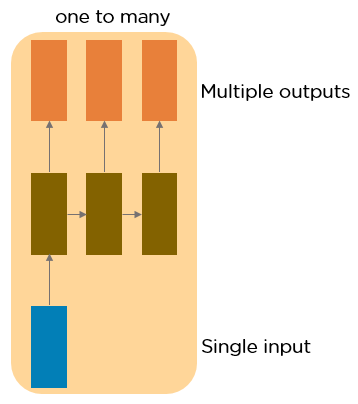
\includegraphics[width=7cm]{chaps/lr/rnn_otm}}
% 	\caption{ساختار \gls{rnn} یک به چند}
% 	\label{fig:ch_lr:rnn_otm}
% \end{figure}
\\

 چند به یک (\lr{many to one}): این نوع از \gls{rnn}، دنباله ایی از ورودی ها را می‌گیرد و یک خروجی تولید می‌کند. تحلیل احساسات مثال خوبی از این نوع شبکه است که یک جمله را به عنوان ورودی می‌گیرد و آن را با احساس مثبت یا منفی طبقه بندی می‌کند.

%
% \begin{figure}[!ht]
% 	\centerline{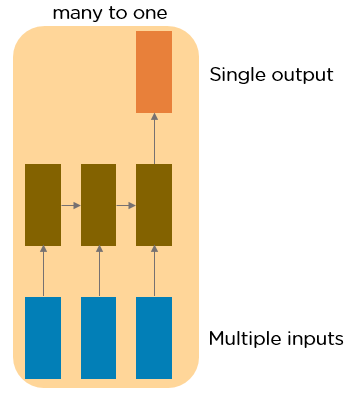
\includegraphics[width=7cm]{chaps/lr/rnn_mto}}
% 	\caption{ساختار \gls{rnn} چند به یک}
% 	\label{fig:ch_lr:rnn_mto}
% \end{figure}
 
 چند به چند (\lr{many to many}): دنباله ایی از ورودی ها را می‌گیرد و دنباله ایی از خروجی ها را تولید می‌کند. ترجمه ماشینی نمونه ایی از این نوع شبکه است.
%\begin{figure}[!ht]
%	\centerline{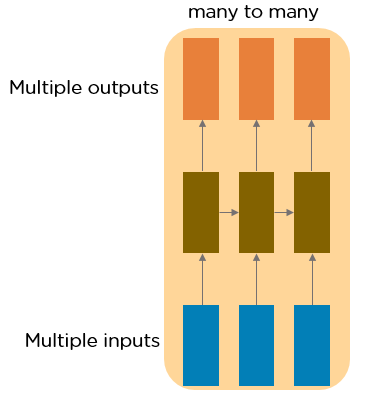
\includegraphics[width=7cm]{chaps/lr/rnn_mtm}}
%	\caption{ساختار \gls{rnn} چند به چند}
%	\label{fig:ch_lr:rnn_mtm}
%\end{figure} 


 \subsection{حافظه‌ی کوتاه‌مدت بلند (\lr{LSTM})}
 شبکه‌های \gls{lstm} یا \lr{LSTM} نسخه‌ی تغییریافته‌ای از شبکه‌های عصبی بازگشتی هستند که یادآوری داده‌های گذشته در آن‌ها تسهیل شده است. مشکل گرادیان کاهشی که در شبکه عصبی بازگشتی وجود داشت نیز در این شبکه‌ها حل شده است. شبکه‌های \lr{LSTM} برای مسائل رده‌بندی، پردازش و پیش‌بینی سری‌های زمانی با استفاده از برچسب‌های زمانی مدت‌های نامعلوم مناسب هستند. این شبکه‌ها مدل را با استفاده از انتشار رو به عقب آموزش می‌دهند. 
 \begin{figure}[!ht]
 	\centerline{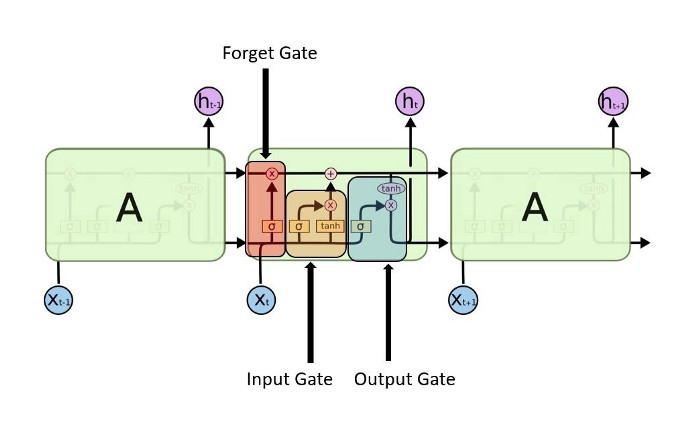
\includegraphics[width=15cm]{chaps/lr/lstm}}
 	\caption{ساختار \lr{LSTM}}
 	\label{fig:ch_lr:lstm}
 \end{figure}
\\
همان‌طور که در شکل \ref{fig:ch_lr:lstm} نمایش داده شده است، در یک شبکه‌ی \lr{LSTM} سه دریچه وجود دارد:
 
\subsubsection*{دریچه‌های \lr{LSTM}}
\textbf{1) دریچه‌ی ورودی}:
با استفاده از این دریچه می‌توان دریافت کدام مقدار از ورودی را باید برای تغییر حافظه به کار برد. تابع \gls{sigmoid} تصمیم می‌گیرد مقادیر بین $0$ و $1$ اجازه‌ی ورود دارند و تابع $\tanh$ با ضریب‌دهی (بین $-1$ تا $+1$) به مقادیر، در مورد اهمیت آن‌ها تصمیم می‌گیرد.
 \begin{equation}
  	\begin{aligned}
  		i_t &= \sigma (W_i \cdot [h_{t-1}, x_t]+b_i)
  		\\
  		\tilde{C}_t &= \tanh(W_C \cdot [h_{t-1}, x_t] + b_C)
  	\end{aligned}
 	\label{eq:ch_lr:lstm_in}
 \end{equation}
 
\textbf{2) دریچه‌ی فراموشی}:
 از طریق این دریچه می‌توان جزئیاتی را که باید از بلوک حذف شوند، تشخیص داد. تصمیم‌گیری در این مورد برعهده‌ی تابع \gls{sigmoid} است. این تابع با توجه به حالت قبلی $h_{t-1}$ و ورودی محتوا $X_t$، عددی بین $0$ تا $1$ به هرکدام از اعداد موجود در حالت سلولی $C_{t-1}$ اختصاص می‌دهد؛ $0$ نشان‌دهنده‌ی حذف آن عدد و $1$ به معنی نگه داشتن آن است.
 \begin{equation}
	f_t = \sigma(W_f\cdot [h_{t-1}, x_t] + b_f)
 	\label{eq:ch_lr:lstm_loss}
 \end{equation}
 
\textbf{3) دریچه‌ی خروجی}:
 ورودی و حافظه‌ی بلوک برای تصمیم‌گیری در مورد خروجی مورد استفاده قرار می‌گیرند. تابع سیگموئید تصمیم می‌گیرد مقادیر بین $0$ و $1$ اجازه‌ی ورود دارند و تابع $\tanh$ با ضریب‌دهی (بین $-1$ تا $+1$) به مقادیر و ضرب آن‌ها در خروجی تابع \gls{sigmoid} در مورد اهمیت آن‌ها تصمیم‌گیری می‌کند.
 \begin{equation}
 	\begin{aligned}
 		o_t &= \sigma (W_o \cdot [h_{t-1}, x_t]+b_o)
 		\\
 		h_t &= o_t \ast \tanh(C_t)
 	\end{aligned}
 	\label{eq:ch_lr:lstm_out}
 \end{equation}

 در حقیقت هدف از طراحی شبکه‌های \lr{LSTM}، حل کردن مشکل وابستگی بلندمدت بود. به این نکته مهم توجه کنید که به یاد سپاری اطلاعات برای بازه‌های زمانی بلند مدت، رفتار پیش‌فرض و عادی شبکه‌های \lr{LSTM} است و ساختار آ‌ن‌ها به صورتی است که اطلاعات خیلی دور را به خوبی یاد می‌گیرند که این ویژگی در ساختار آن‌ها نهفته است.
 
 همه شبکه‌های عصبی بازگشتی به شکل دنباله‌ای (زنجیره‌ای) تکرار شونده از ماژول‌های (واحد‌های) شبکه‌های عصبی هستند. در شبکه‌های عصبی بازگشتی استاندارد، این ماژول‌های تکرار شونده ساختار ساده‌ای دارند، برای مثال تنها شامل یک لایه تانژانتِ هایپربولیک ($\tanh$) هستند.
 
 \begin{figure}[!ht]
 	\centerline{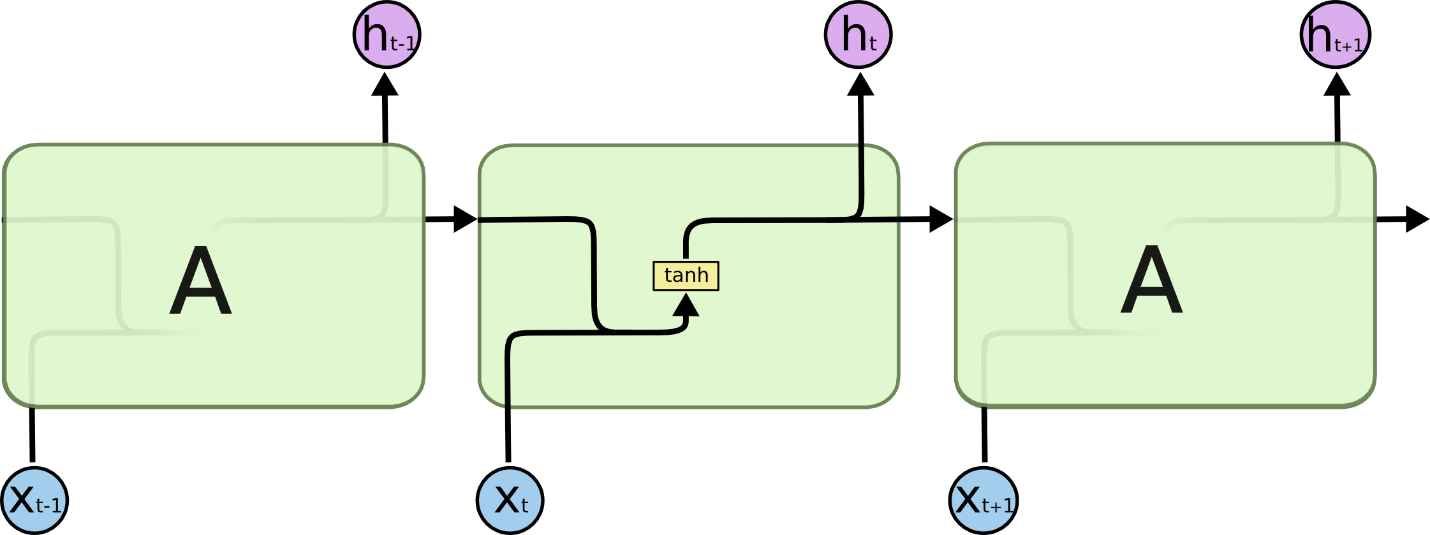
\includegraphics[width=14cm]{chaps/lr/rnn_chain}}
 	\caption{
ماژول‌های تکرار شونده در شبکه‌های عصبی بازگشتی استاندارد فقط دارای یک لایه هستند.
 	}
 	\label{fig:ch_lr:rnn_chain}
 \end{figure}
 
 شبکه‌های \lr{LSTM} نیز چنین ساختار دنباله یا زنجیره‌مانندی دارند ولی ماژولِ تکرار شونده ساختار متفاوتی دارد. به جای داشتن تنها یک لایه شبکه عصبی، 4 لایه دارند که طبق ساختار ویژه‌ای با یکدیگر در تعامل و ارتباط هستند.
 \begin{figure}[!ht]
	\centerline{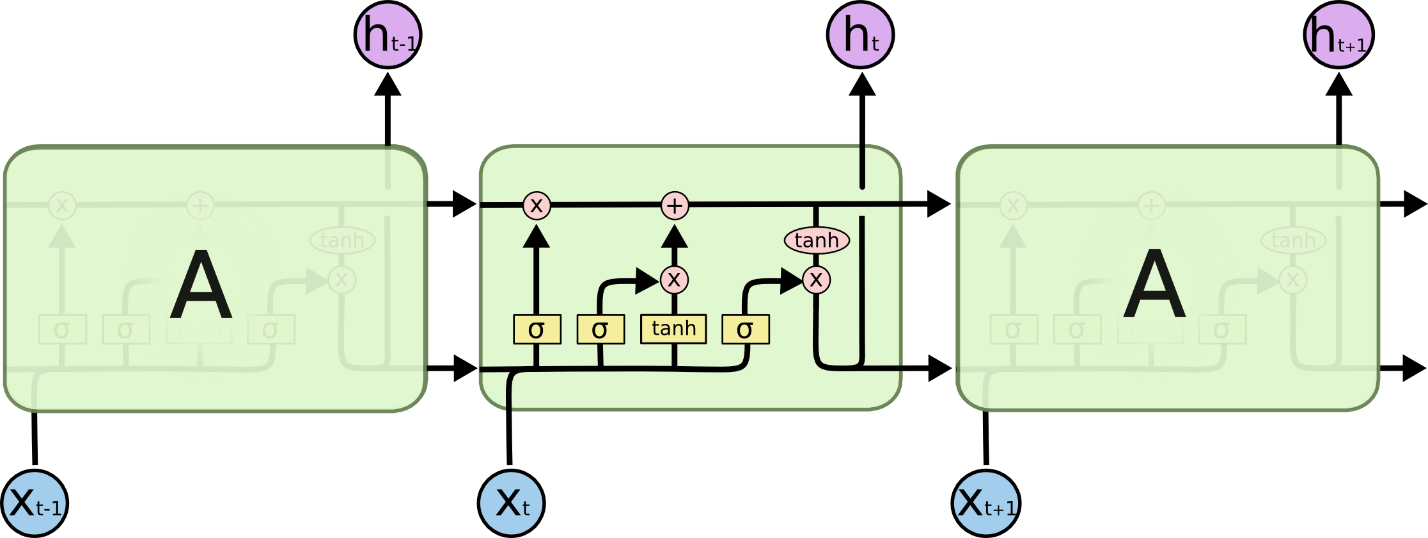
\includegraphics[width=14cm]{chaps/lr/rnn_inside}}
	\caption{
		ماژول‌های تکرار شونده در \lr{LSTM}ها دارای 4 لایه هستند که با هم در تعامل می‌باشند.
	}
	\label{fig:ch_lr:rnn_inside}
\end{figure} 
در ادامه قدم به قدم ساختار شبکه‌های \gls{lstm} را توضیح خواهیم داد. اما در ابتدا معنی هر کدام از شکل‌ و علامت‌هایی را که از آن‌ها استفاده خواهیم کرد توضیح می‌دهیم.
  \begin{figure}[!ht]
 	\centerline{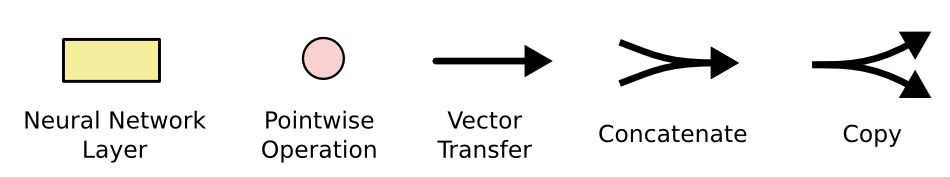
\includegraphics[width=14cm]{chaps/lr/lstm_legend}}
 	\caption{
 		اشکال از راست به چپ به تریب برابر هستند با: کپی کردن، وصل کردن، بردار انتقال، عملیات نقطه به نقطه، یک لایه‌ی شبکه عصبی.
 	}
 	\label{fig:ch_lr:lstm_legend}
 \end{figure} 
 در شکل \ref{fig:ch_lr:lstm_legend}، هر خط یک بردار را به صورت کامل از خروجی یک گره به ورودی گره دیگر انتقال می‌دهد. دایره‌های صورتی نمایش دهنده عملیات‌های نقطه‌ به نقطه مانند «جمع کردن دو بردار» هستند. مستطیل‌های زرد، لایه‌‌های شبکه‌های عصبی هستند که شبکه پارامتر‌های آن‌ها را یاد می‌گیرد. خط‌هایی که با هم ادغام می‌شوند نشان‌دهنده \gls{concatenation} و خط‌هایی که چند شاخه می‌شوند نشان دهنده‌ای این موضوع است که محتوای آن‌ها کپی و به بخش‌های مختلف ارسال می‌شود.
\\
\\
 عنصر اصلی \lr{LSTM}ها سلول حالت\LTRfootnote{Cell state} است که در حقیقت یک خط افقی است که در بالای شکل \ref{fig:ch_lr:lstm_cellState1} قرار دارد.
 سلول حالت را می‌توان به صورت یک تسمه نقاله تصور کرد که از اول تا آخر دنباله یا همان زنجیره با تعاملات خطیِ جزئی در حرکت است (یعنی ساختار آن بسیار ساده است و تغییرات کمی در آن اتفاق می‌افتد).
   \begin{figure}[!ht]
 	\centerline{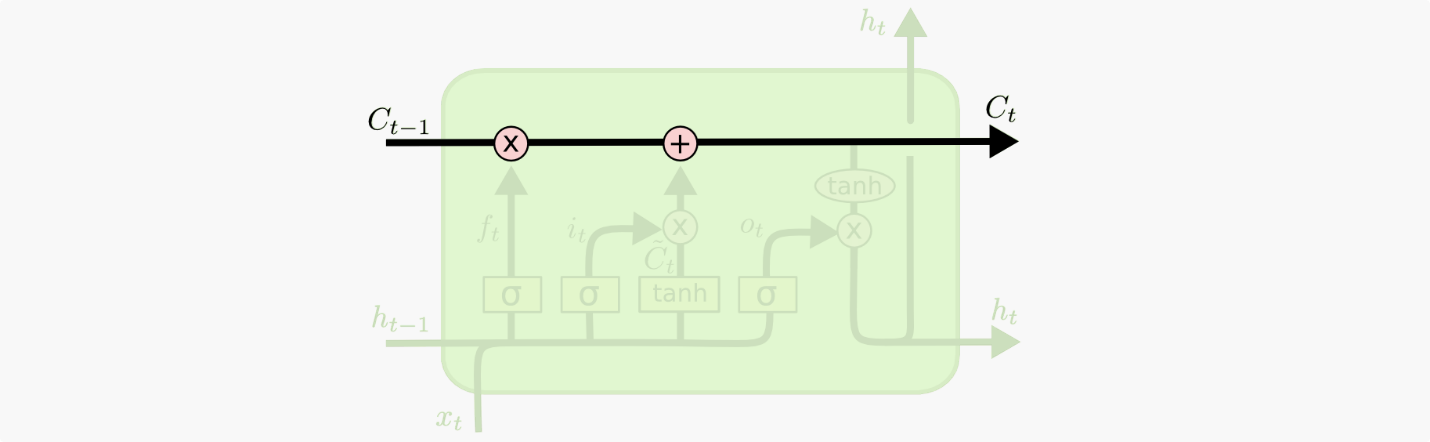
\includegraphics[width=15cm]{chaps/lr/lstm_cellState1}}
 	\caption{
 		سلول حالت در ماژول \lr{LSTM}
 	}
 	\label{fig:ch_lr:lstm_cellState1}
 \end{figure} 
\\
 \lr{LSTM} 
 این توانائی را دارد که اطلاعات جدیدی را به سلول حالت اضافه یا اطلاعات آن را حذف کنید. این کار توسط ساختارهای دقیقی به نام \glspl{gate} انجام می‌شود. \glspl{gate}‌ راهی هستند برای ورود اختیاری اطلاعات. آن‌ها از یک لایه شبکه عصبیِ \gls{sigmoid} به همراه یک عملگر ضرب نقطه به نقطه تشکلیل شده‌اند.
 \begin{figure}[!ht]
 	\centerline{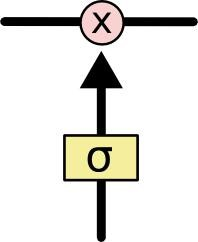
\includegraphics[width=3cm]{chaps/lr/lstm_2}}
 	\caption{
 		نمایی از نحوه تاثیر و ورود اطلاعات به سلول حالت
 	}
 	\label{fig:ch_lr:lstm_2}
 \end{figure} 
\\
 خروجی لایه \gls{sigmoid} عددی بین صفر و یک است، که نشان می‌دهد چه مقدار از وروی باید به خروجی ارسال شود. مقدار صفر یعنی هیچ اطلاعاتی نباید به خروجی ارسال شود در حالی که مقدار یک یعنی تمام ورودی به خروجی ارسال شود!
 \\
 \\
 \lr{LSTM}
  دارای 3 \gls{gate} مشابه برای کنترل مقدار سلول حالت است که در ادامه به بررسی قدم به قدمِ آن‌ها از لحظه ورود تا خروج اطلاعات خواهیم پرداخت.
  \\
 قدم اول در \lr{LSTM} تصمیم در مورد اطلاعاتی است که می‌خواهیم آن‌ها را از سلول حالت پاک کنیم. این تصمیم توسط یک لایه \gls{sigmoid} به نام «دروازه فراموشی\LTRfootnote{Forget gate}» انجام می‌شود. این \gls{gate} با توجه به مقادیر $h_{t-1}$ و $x_t$، برای هر عدد، مقدار صفر یا یک را در سلول حالتِ $C_{t-1}$ به خروجی می‌برد. مقدار یک یعنی به صورت کامل مقدار حال حاضرِ سلول حالت $C_{t-1}$ را به $C_t$ انتقال داده شود و مقدار صفر یعنی به صورت کامل اطلاعات سلول حالت کنونی $C_{t-1}$ را پاک شود و هیچ مقداری از آن  به $C_t$ برده نشود. بیاید به مثال قبلی‌مان که یک مدل زبانی‌ای بود که در آن تلاش داشتیم کلمه بعدی را بر اساس همه کلمه‌های قبلی حدس بزنیم، برگردیم. در چنین مسأله‌ای، سلول حالت ممکن است دربردارنده جنسیت فاعل کنونی باشد، که با توجه به آن می‌توانیم تشخیص دهیم از چه ضمیری باید استفاده کنیم. زمانی که یک فاعل جدید در جمله ظاهر می‌شود، می‌بایست جنسیت فاعل قبلی حذف شود.
 \begin{figure}[!ht]
	\centerline{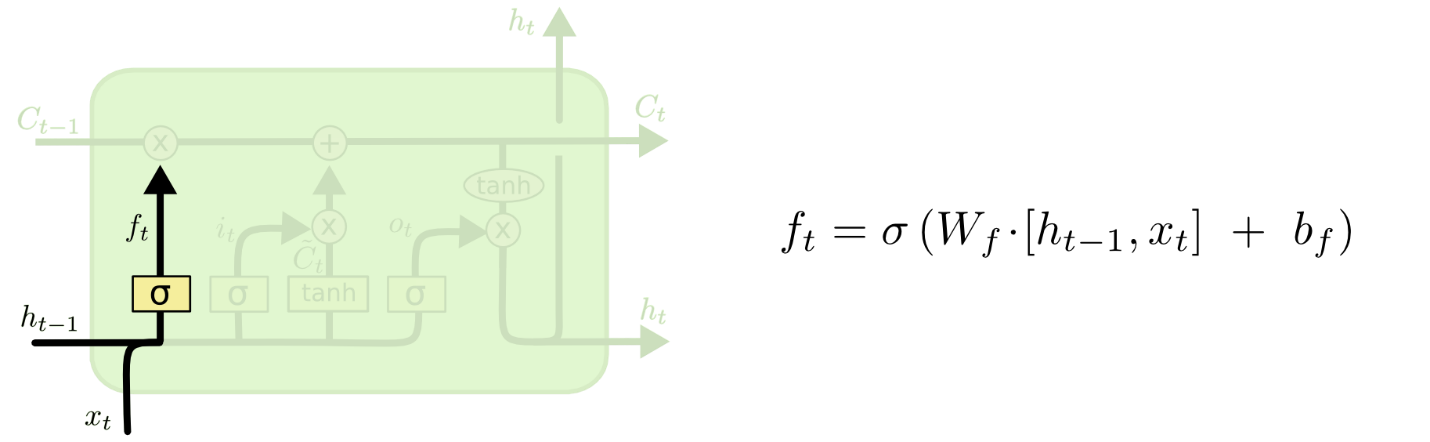
\includegraphics[width=15cm]{chaps/lr/lstm_3}}
	\caption{
		قدم اول در پاک کردن اطلاعات از سلول حالت در وضعیت ورودی
	}
	\label{fig:ch_lr:lstm_3}
\end{figure} 
\\
قدم بعدی این است که تصمیم بگیریم چه اطلاعات جدیدی را می‌خواهیم در سلول حالت ذخیره کنیم. این تصمیم دو بخشی است. ابتدا یک لایه سیگموید به نام دروازه ورودی\LTRfootnote{Input gate} داریم که تصمیم می‌گیرد چه مقادیری به‌روز خواهند شد. مرحله بعدی یک لایه تانژانت هایپربولیک است که برداری از مقادیر به نام $\tilde{C}_t$ می‌سازد که می‌توان آن‌ها را به سلول حالت اضافه کرد. در مرحله بعد، ما این دو مرحله را با هم ترکیب می‌کنیم تا مقدار سلول حالت را به‌روز کنیم.
\\
در مثال مدل زبانی‌ای که پیش‌تر داشتیم، قصد داریم جنسیت فاعل جدید را به سلول حالت اضافه کنیم تا جایگزین جنسیت فاعل قبلی شود که در مرحله قبلی تصمیم گرفتیم آن را فراموش کنیم.
 \begin{figure}[!ht]
	\centerline{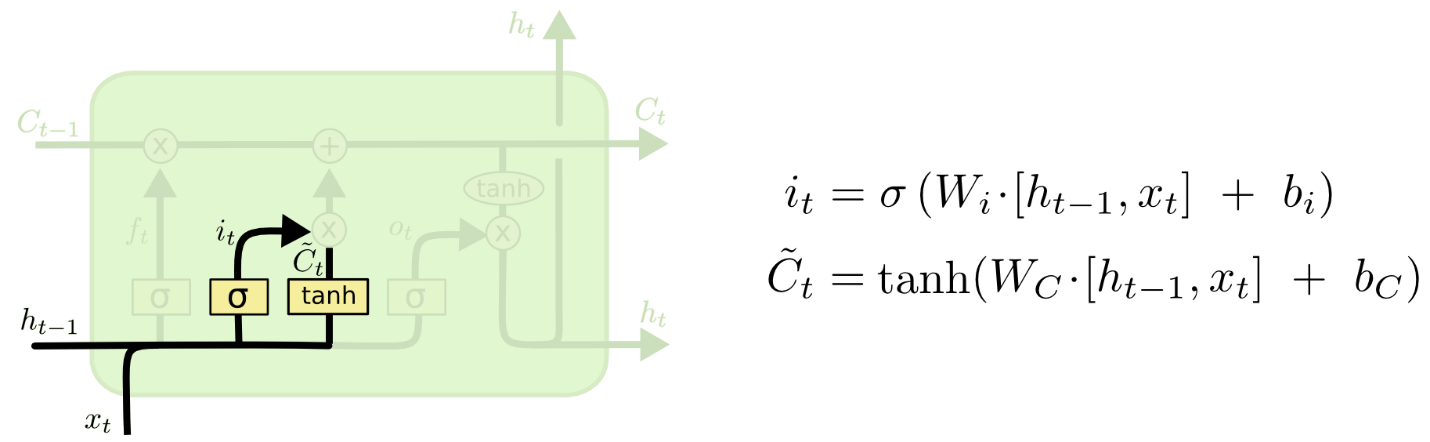
\includegraphics[width=15cm]{chaps/lr/lstm_4}}
	\caption{
		قدم دوم در اضافه کردن اطلاعات جدید به سلول حالت
	}
	\label{fig:ch_lr:lstm_4}
\end{figure} 
\\
حال زمان آن فرا رسیده است که سلول حالت قدیمی یعنی $C_{t-1}$ را سلول حالت جدید یعنی $C_t$ به‌روز کنیم. در مراحل قبلی تصمیم گرفته شد که چه کنیم و در حال حاضر تنها لازم است تصمیماتی را که گرفته شد عملی کنیم.
\\
ما مقدار قبلی سلول حالت را در $f_t$ ضرب می‌کنیم که یعنی فراموش کردن اطلاعاتی که پیش‌تر تصمیم گرفتیم آن‌ها را فراموش کنیم. سپس $i_t \ast \tilde{C}_t$ را به آن اضافه می‌کنیم. در حال حاضر مقادیر جدید سلول حالت با توجه به تصمیماتی که پیش‌تر گرفته شده بود بدست آمده‌اند. در مثال مدل زبانی، اینجا دقیقاً جائی است که اطلاعاتی که در مورد جنسیت قبلی داشتیم را دور می‌ریزیم و اطلاعات جدید را اضافه می‌کنیم.
 \begin{figure}[!ht]
	\centerline{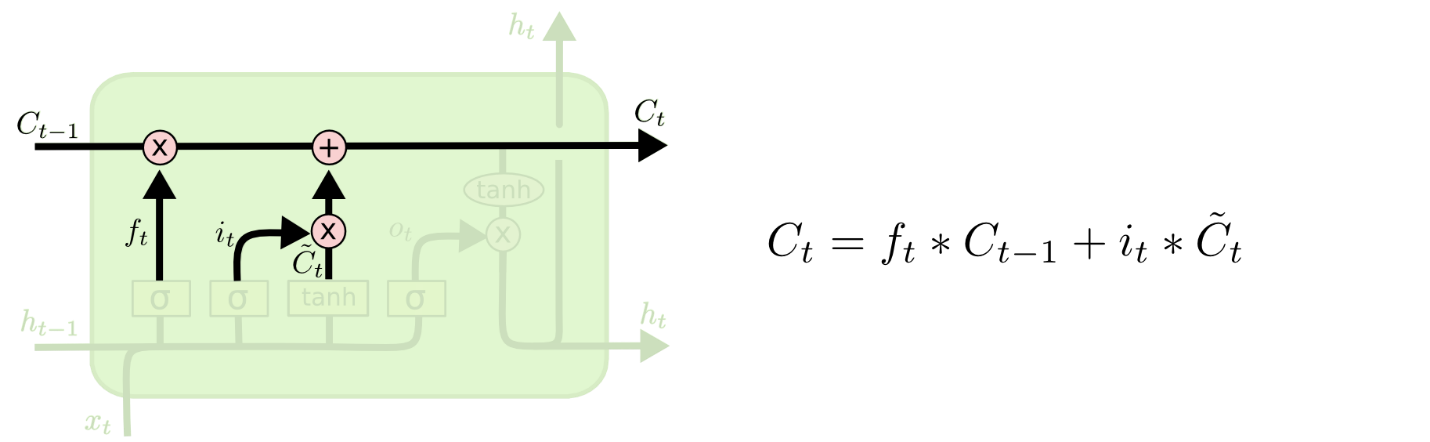
\includegraphics[width=15cm]{chaps/lr/lstm_5}}
	\caption{
		به‌روز رسانی اطلاعات در سلول حالت
	}
	\label{fig:ch_lr:lstm_5}
\end{figure} 
\\
در نهایت باید تصمیم بگیریم قرار است چه اطلاعاتی را به خروجی ببریم. این خروجی با در نظر گرفتن مقدار سلول حالت خواهد بود، ولی از فیلتر مشخصی عبور خواهد کرد. در ابتدا، یک لایه سیگموید داریم که تصمیم می‌گیرد چه بخشی از سلول حالت قرار است به خروجی برده شود. سپس مقدار سلول حالت (پس از به‌روز شدن در مراحل قبلی) را به یک لایه تانژانت هایپربولیک (تا مقادیر بین $-1$ و $+1$ باشند) می‌دهیم و مقدار آن را در خروجی لایه \gls{sigmoid} قبلی ضرب می‌کنیم تا تنها بخش‌هایی که مد نظرمان است به خروجی برود.
\\
در مثال مدل زبانی، با توجه به اینکه تنها فاعل را دیده‌است، در صورتی که بخواهیم کلمه بعدی را حدس بزنیم، ممکن است بخواهد اطلاعاتی در ارتباط با فعل را به خروجی ببرد. برای مثال ممکن است اینکه فاعل مفرد یا جمع است را به خروجی ببرد، که ما با توجه به آن بدانیم فعل به چه فرمی خواهد بود.
 \begin{figure}[!ht]
	\centerline{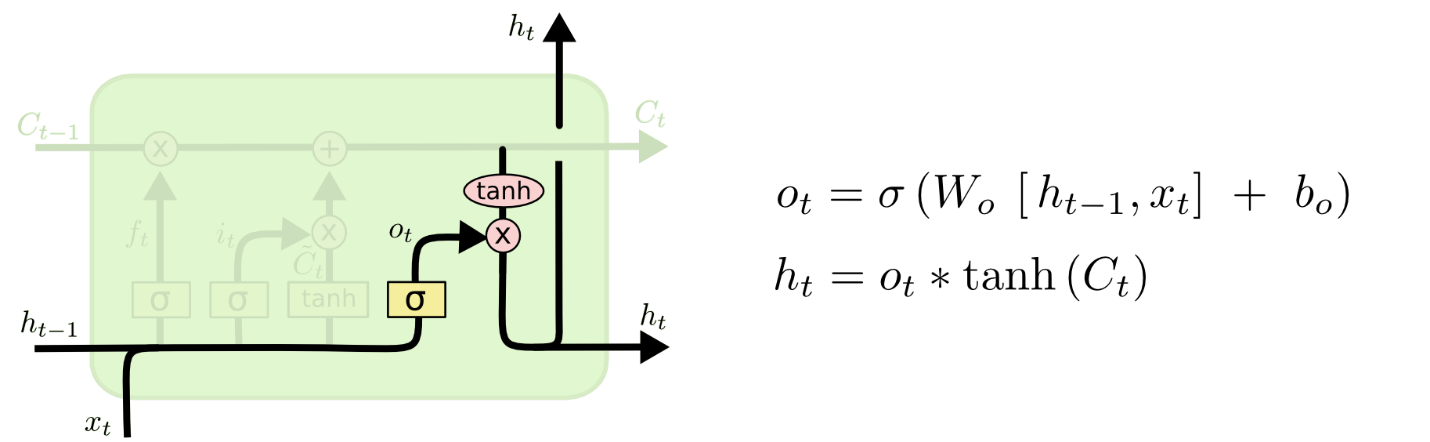
\includegraphics[width=15cm]{chaps/lr/lstm_6}}
	\caption{
		قدم نهایی برای تولید خروجی ماژول \lr{LSTM}
	}
	\label{fig:ch_lr:lstm_6}
\end{figure} 
 
 \section{\gls{reinforcementlearning}}
 
 \subsection{مقدمه و بیشینه تاریخی}
% ادوارد ثورندایک\LTRfootnote{Edward Thorndike} پدر روانشناسی مدرن در سال 1874 میلادی در ایالت ماساچوست آمریکا متولد شد. وی در اوایل قرن 20 میلادی آزمایشی انجام داد که باعث ارائه قانون اثر شد. او برای این آزمایش، گربه ای را در جعبه ای موسوم به جعبه معما قرار داد. هر کوشش درستی، از این گربه برای نجات از جعبه صورت می‌گرفت، باعث میشد ثورندایک به عنوان پاداش به او غذا بدهد. به تدریج گربه به کارهای درست خود پی برد و آنها را تکرار کرد، تا جایی که دیگر هیچ کار اشتباهی نمی کرد و بلاخره موفق به خروج از جعبه شد. ثورندایک در سال 1912 به ریاست انجمن روانشناسان، در سال 1917 به عضویت انجمن علوم، در سال 1934به ریاست انجمن علوم پیشرفته نایل آمد و در سال 1947 در سن 74 سالگی، بدرود حیات گفت. در سال 2002 رتبه ای از برترین روانشناسان تاریخ ارائه شد که ثورندایک جزء 10 روانشناس برتر تاریخ قرار گرفت. می‌توان مهم ترین کشف وی را، اثبات وجود یادگیری تقویتی در روانشناسی دانست.
 
 شاید ریچارد بلمن\LTRfootnote{Richard E. Bellman} (مخترع الگوریتم بلمن-فورد) را بتوان اولین کسی دانست که یادگیری تقویتی را وارد هوش مصنوعی ساخت. در اوایل دهه 1950 بلمن مسئله ای با عنوان «کنترل بهینه» را مطرح ساخت که با استفاده از روش های پویا در برنامه‌ریزی پویا کنترل کننده‌ها را به سمت نتیجه بهینه رهنمون می‌شد. در اواخر دهه 50 میلادی مینسکی در پایان نامه دکتری خود روش های محاسبات آزمون و خطا توسط مفهوم یادگیری تقویتی را مطرح نمود و الگوریتم های یادگیری تقویتی را پایه ریزی کرد. در کل دهه 50 میلادی را میتوان دهه تشکیل الگوریتم های محاسباتی اولیه یادگیری تقویتی دانست. در دهه 60 میلادی اولین کابرد های یادگیری تقویتی به وقوع پیوستند. در اولین تلاش ها فارلی و کلارک از یادگیری تقویتی برای تشخیص الگو استفاده کردند بدین صورت که هر بار برنامه نتیجه بهتری به دست می‌آمد او را تشویق می‌کردند. در اواخر دهه 60 میلادی، یادگیری نظارتی از یادگیری تقویتی ، مشتق شد. در یادگیری نظارتی طراح نتیجه نهایی را در دست دارد و از هوش مصنوعی می‌خواهد هر بار مسیر بین ورودی و نتیجه را طراحی کرده و هربار که برنامه، مسیر بهتری به دست می‌آورد، تشویق می‌شود. همچنین طراح نظارت مستقیم بر عملکرد عامل دارد.

 \subsection{مفاهیم و تعاریف}
 در اینجا در ابتدا مروری بر مطالب پیشین شده و سپس به سرفصل اصلی پرداخته شده است.
 یادگیری تقویتی چیست؟
 تفاوت یادگیری تقویتی با \gls{supervisedlearning} و \gls{unsupervised} در دو نقطه است:
 \begin{enumerate}
 	\item \gls{environment}: محیطی همانند هزارتو، بازی ویدیویی، بازار سهام و ...
 	\item \gls{agent}: همان هوش مصنوعی است که یاد می گیرد، چگونه عمل کند و در محیط به صورت موفقیت آمیز عمل کند.
 \end{enumerate}
 عامل از طریق تعامل تکراری با محیط، یاد می‌گیرد چگونه در محیط عمل کند. عامل یاد می‌گیرد که کدام اعمال در حالت مشخصی ارزشمندتر و مطلوب‌تر هستند. با انجام دادن عمل توسط عامل و دریافت نتایج، حالت محیط براساس پاداش دریافتی تغییر خواهد کرد. حلقه تکرار اعمال، حالات‌های پاداش به شکل 	\ref{fig:ch_lr:ae_rl} قابل تصور است.
 
 \begin{figure}[!ht]
 	\centerline{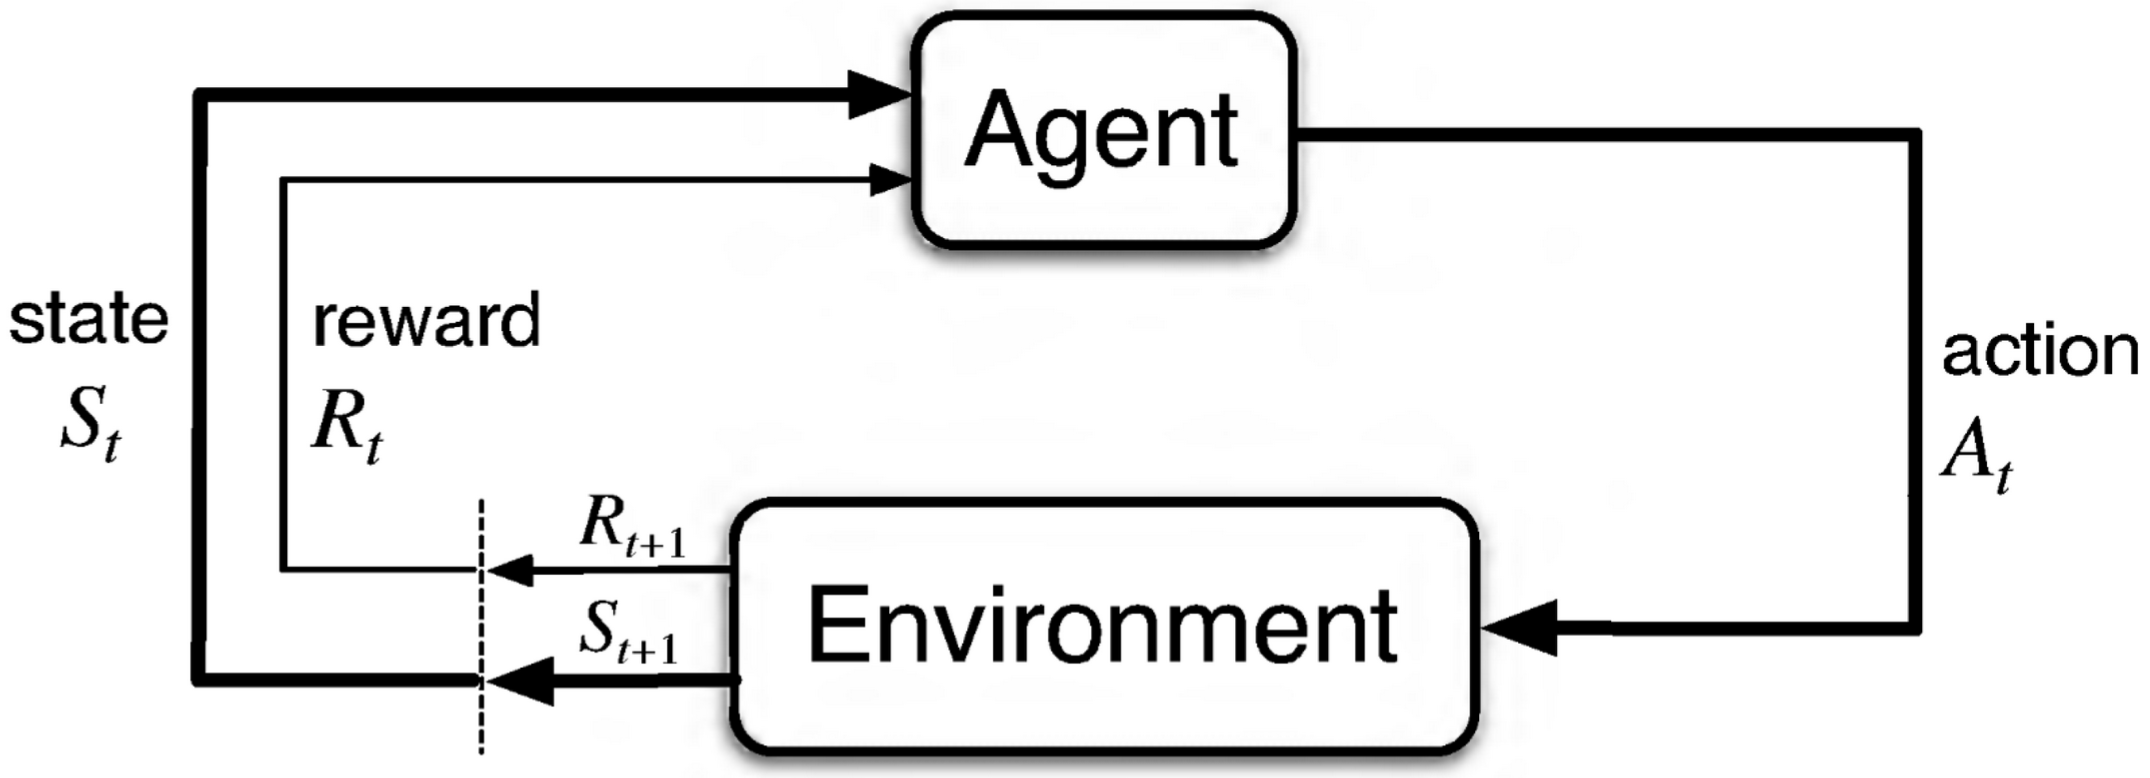
\includegraphics[width=11cm]{chaps/lr/ae_rl}}
 	\caption{تعامل عامل$-$محیط در یک فرآیند تصمیم مارکوف.}
 	\label{fig:ch_lr:ae_rl}
 \end{figure}
\noindent
 هدف عامل این است که پاداش تجمعی دریافتی مورد انتظارش را به حداکثر برساند.
 \subsubsection{ معادله بلمن}
 این معادله یک مفهوم اساسی در یادگیری تقویتی است:
 $$ s: \text{حالت}\qquad a:\ \text{عمل}\qquad R:\ \text{ پاداش}\qquad  \gamma:\ \text{فاکتور تخفیف یا کاهش}$$
ارزش انجام عمل با به تاخیر افتادن آن کاهش پیدا می کند.
 \\
 به منظور حل یک مسئله در یادگیری تقویتی با روش \lr{Q-learning} باید جدول \lr{Q} متناظر با حالات مسئله را  ساخت. این جدول یک جدول جست‌جو\LTRfootnote{lookup-table} است که پاداش آتی مورد انتظار برای هر عمل در هر حالت را نشان می‌دهد. با استفاده از این جدول می‌توان بهترین عمل را در هر حالتی انتخاب کرد.
 چگونه باید حداکثر پاداش مورد انتظار در هر حالت را حساب کرد؟ به عبارت دیگر چگونه می توان مقادیر جدول \lr{Q} را تعیین کرد؟
 \\
  مقادیر این جدول با استفاده از الگوریتم \lr{Q-learning} به صورت تکرار به روزرسانی خواهند شد. رابطه مورد نیاز برای به‌روزرسانی این جدول در محیط‌های قطعی به صورت زیر است. در این رابطه از معادله بلمن استفاده شده است.
 \begin{equation}
 	V(s) = \max_{a}\big(R(s,a)+\gamma V(s')\big)
 \end{equation}
 طبق معادله داده شده:
 \begin{itemize}
 	\item  ارزش حالت مشخص برابر است با انتخاب عملی(از میان تمام  اعمال موجود) که منجر به بیشترین ارزش خواهد شد. 
 	\item  با انجام عمل $a$ در حالت s و جمع کردن آن با ضریب کاهش $\gamma$ می‌توان به ارزش انجام عمل رسید. 
 	\item  با انجام عمل $a$ عامل به حالت جدید $s'$ انتقال می‌یابد.
 \end{itemize}

\subsubsection{\glspl{mdp}}
در ابتدا تفاوت جست‌وجوی قطعی و غیر قطعی را شرح می‌دهیم.\\
 جست‌وجوی قطعی: در این نوع اکتشاف اگر عامل، عمل $a$ را انتخاب کند با احتمال $100\%$  آن را انجام خواهد داد.\\
 جست‌وجوی غیر قطعی: به نوعی در محیط تصادفی است و در این نوع اکتشاف اگر عامل عمل $a$ را انتخاب کند ممکن است با احتمال $\epsilon>0$ اعمال دیگر را انجام دهد. 
 \\
\textbf{فرآیندهای مارکوف}
\\
 \gls{mdp} خاصیت مارکوف را داراست، اگر توزیع احتمال شرطی حالات آینده فرایند (به شرط حالات گذشته و حالات فعلی) تنها وابسته به حالت فعلی باشد و نه دنباله ای از رویدادهای پیشین آن. به منظور ساده‌سازی آن، آن چیزی که در آینده اتفاق می افتد به ان چیزی که در گذشته روی داده وابسته نیست. 
\\
\textbf{\gls{mdp}}
چهارچوبی است که عامل به منظور عمل کردن در محیط نسبتا تصادفی از آن استفاده می‌کند. به دلیل اینکه محیط تصادفی است، به صورت دقیق حالت بعدی $s'$ معلوم نیست. پس از مقدار مورد انتظار یا امید ریاضی حالت بعد استفاده می‌شود که در این صورت معادله بلمن برای حالت یک محیط غیر قطعی به صورت رابطه زیر خواهد بود.
  \begin{equation}
 	V(s) = \max_{a}\big(R(s,a)+\gamma \sum_{s'}P(s,a,s')V(s')\big)
 	\label{eq:ch_lr:bellman}
 \end{equation}


\subsection{یادگیری-\lr{Q}}
یک الگوریتم یادگیری مبتنی بر ارزش در یادگیری تقویتی است. یادگیری-\lr{Q} به عامل اجازه می‌دهد که از پاداش محیط برای یادگیری استفاده کند و به مرور زمان بهترین عمل در حالت داده شده انتخاب شود. عامل از جدول پاداش برای یادگیری استفاده می‌کند. عامل براساس عملی که انجام می‌دهد، پاداشی را در حالت فعلی دریافت خواهد کرد، سپس ارزش-\lr{Q} را به‌روزرسانی می‌کند تا بداند که این عمل مفید بوده است.
مقادیر ذخیره شده در جدول \lr{Q}،  ارزش-\lr{Q} نامیده می‌شوند. این مقادیر را می‌توان به صورت زوج مرتب  
(حالت، عمل)
نگاشت داد. ارزش-\lr{Q} برای ترکیب حالت-عمل نمایانگر "کیفیت" عملی است که می‌توان در آن حالت انجام داد. مقادیر بهتر ارزش-\lr{Q} نشان دهنده شانس بیشتر برای دریافت پاداش بیشتر است. این مقادیر  در ابتدا می‌توانند به صورت تصادفی مقداردهی اولیه شوند. عامل با در معرض محیط قرار گرفتن و دریافت پاداش‌های مختلف از محیط و انجام  اعمال مختلف، میتواند مقادیر  ارزش-\lr{Q} را به‌روزرسانی کند.

در بخش قبل به معادله \ref{eq:ch_lr:bellman} توجه کنید. در این معادله، در یادگیری-\lr{Q}، در عوض اینکه از $V(s)$ ارزش هر حالت استفاده شود از ارزش زوج حالت-عمل $Q(s,a)$ استفاده می‌شود. می‌توان گفت که ارزش-\lr{Q}  به معنای کیفیت هر عمل است. 
\\
% معادله ارزش حالت $s$ در محیط غیرقطعی به رابطه زیر است.
% \begin{equation}
% 	V(s) = \max_{a}\big(R(s,a)+\gamma \sum_{s'}P(s,a,s')V(s')\big)
% \end{equation}
برای بدست آوردن معادله $Q(s,a)$:\\
با انجام دادن یک عمل پاداش دریافتی در حالت s برابر است با $R(s,a)$\\
عامل به حالت $s'$ انتقال یافته و از آنجایی که عامل می‌تواند در چندین حالت قرار بگیرد، مقدار مورد انتطار حالت بعدی به پاداش اضافه خواهد شد.
\begin{equation}
	Q(s,a) = R(s,a)+\gamma \sum_{s'}P(s,a,s')V(s')
\end{equation}
شباهت معادله بالا با معادله بلمن به این دلیل است که ارزش حالت $s$ برابر است با حداکثر تمام مقادیر ارزش-\lr{Q}
با جایگزین کردن $V(s')$ با $Q(s',a')$ معادله زیر بدست می آید:
\begin{equation}
	V(s) = R(s,a)+\gamma \sum_{s'}P(s,a,s')\max_{a'}\big(Q(s',a')\big)
\end{equation}
این معادله بازگشتی ارزش-\lr{Q} است.

\subsubsection{\gls{temporaldifference}}
از انجایی که به دلیل غیرقطعی بودن محیط، محاسبه کردن ارزش هر حالت بسیار مشکل است، از تفاضل زمانی برای حل این مشکل استفاده می‌شود.
به منظور راحتی، از معادله قطعی بلمن استفاده می‌شود اما کماکان محیط غیرقطعی است،
\begin{equation}
	V(s) = R(s,a)+\gamma \max_{a'}\big(Q(s',a')\big)
\end{equation}
\gls{temporaldifference} به صورت زیر تعریف می‌شود.
\begin{equation}
	TD(s, a) = \max_{a}\big(R(s,a)+\gamma V(s')\big) - Q_{t-1}(s,a)
\end{equation}
جمله سمت راست در رابطه بالا، مقدار ارزش-\lr{Q} پیشین است و دو جمله سمت چپ بیان‌گر پاداش دریافتی پس از انجام عمل $a$ می‌باشد (که مقدار جدید ارزش-\lr{Q} است).
سوالی که اینجا مطرح می‌شود این است که آیا بین این مقادیر در زمان تفاوتی وجود دارد؟ بله و از این اختلاف استفاده می‌شود که به صورت رابطه \gls{temporaldifference} برای محاسبه ارزش-\lr{Q}
\begin{equation}
	Q_{t}(s,a) = Q_{t-1}(s,a) - \alpha TD_t(s,a)
\end{equation}
می‌باشد، که در اینجا $\alpha$ نرخ یادگیری است. این رابطه نحوه آپدیت ارزش-\lr{Q} در زمان را نشان می‌دهد. با جایگزین کردن تفاضل زمانی در معادله بالا معادله زیر بدست می‌آید.
\begin{equation}
	Q_{t}(s,a) = Q_{t-1}(s,a) - \alpha \left( \max_{a}\big(R(s,a)+\gamma V(s')\big) - Q_{t-1}(s,a) \right) 
\end{equation}


\subsection{\gls{deepqlearning}}
استفاده از شبکه های عصبی برای مسائل \gls{reinforcementlearning}:
حالت مورد نظر را از چندین لایه شبکه عبور داده و خروجی ارزش-\lr{Q} بدست خواهد آمد. در شکل \ref{fig:ch_lr:deepql_vs_ql} مقایسه‌ای از
 \lr{Q-learning} با \lr{Deep Q-learning}
  انجام داده شده است.
  \begin{figure}[!ht]
	\centerline{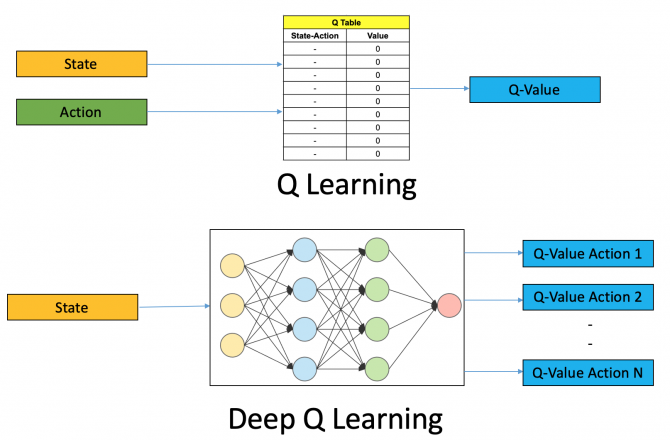
\includegraphics[width=15cm]{chaps/lr/deepql_vs_ql}}
	\caption{مقایسه‌ای از \lr{Q-learning} با \lr{Deep Q-learning}.}
	\label{fig:ch_lr:deepql_vs_ql}
\end{figure} 
 در حالت عادی هدف به طور پیوسته در هر تکرار تغییر خواهد کرد. اما در مسائل یادگیری عمیق این تغییر وجود ندارد و یادگیری پایدار است. 
از انجایی که از یک شبکه برای محاسبه ارزش پیش‌بینی شده و ارزش هدف استفاده می‌شود، ممکن است واگرایی زیادی بین این دو وجود داشته باشد. پس در \gls{deepqlearning} از دو شبکه به جای یک شبکه استفاده می‌شود. از شبکه دیگری برای تخمین هدف استفاده می‌شود. این شبکه معماری یکسانی دارد و به عنوان تابع تخمین استفاده می‌شود که پارامترهایش ثابت شده‌اند و تغییر نخواهند کرد. شکل \ref{alg:ch_lr:deepqlearning} شمایی از این دو شبکه را در این موضوع نشان می‌دهد.
  \begin{figure}[!ht]
	\centerline{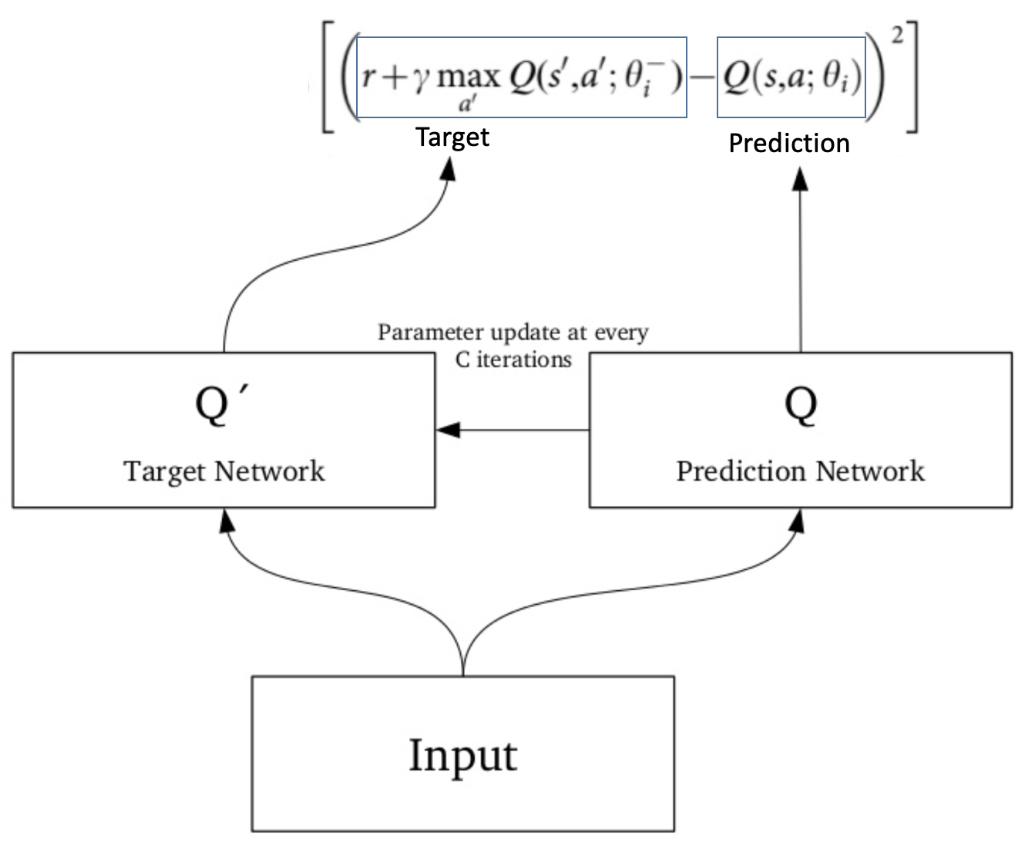
\includegraphics[width=11cm]{chaps/lr/deepqlearning}}
	\caption{نمایی از ساختار \gls{deepqlearning}}
	\label{alg:ch_lr:deepqlearning}
\end{figure} 
 پس از هر $C$ تکرار، پارامترهای شبکه پیش‌بینی به شبکه هدف کپی می‌شوند. این کار منجر به روال آموزش پایدار خواهد شد. 
در ادامه در الگوریتم \ref{alg:ch_lr:deepqlearningalg} شبه‌کد \gls{deepqlearning} آورده شده است.
%reference: https://www.analyticsvidhya.com/blog/2019/04/introduction-deep-q-learning-python/
\begin{algorithm}
	\caption{\gls{deepqlearning} به همراه بازآزمایش}
	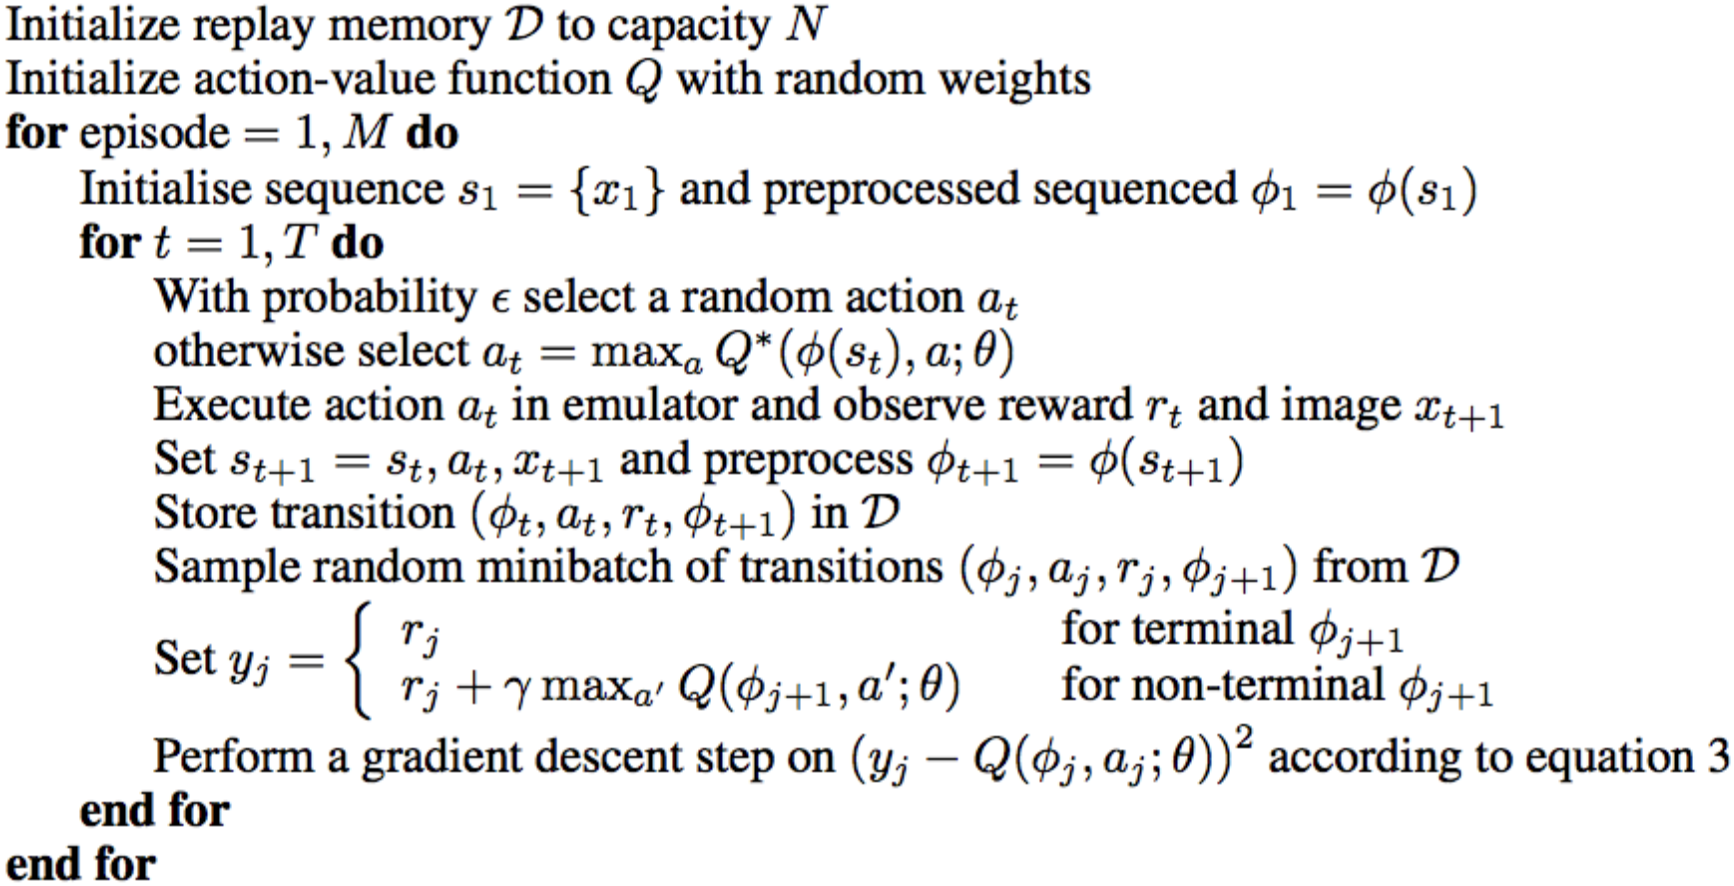
\includegraphics[width=15cm]{chaps/lr/deepqlearningalg}
	\label{alg:ch_lr:deepqlearningalg}
\end{algorithm}

در ادامه دلیل استفاده از \gls{deepqlearning} و مزیت آن بر یادگیری-\lr{Q} را بیان می‌کنیم.
در صورتی که محیط نسبتا ساده باشد الگوریتم  یادگیری-\lr{Q} به خوبی عمل می‌کند، اما در صورتی که تعداد حالات و اعمال انتخابی توسط عامل زیاد شوند، از \gls{deeplearning} به عنوان تابع تخمین زن استفاده می‌شود.
نحوه تغییر معادله بلمن با استفاده از \gls{deepqlearning} در ادامه توضیح داده شده است. 
\\
در مساله هزارتو چهار جهت حرکتی بالا، پایین، چپ و راست امکان‌پذیر است پس شبکه عصبی باید 4 مقدار را پیش‌بینی کند. شبکه می‌تواند 4 مقدار محاسبه شده فعلی را  با 4 مقدار محاسبه شده در قبل مقایسه کند:
$Q_1$ با $Q_{Target1}$ یا $Q_2$ با $Q_{Target2}$ و ...
از انجایی که شبکه های عصبی با به‌روزرسانی وزن‌های کار می‌کنند، باید معادله \gls{temporaldifference} را با این به‌روزرسانی‌ها تطبیق داد. پس می‌توان با محاسبه کردن خطای،
\begin{equation}
	L = \sum (Q - Q_{Target})^2
\end{equation}
و سپس از \gls{backpropagation} یا \gls{stochasticgradientdescent} برای آپدیت وزن‌ها استفاده کرد. با توجه به ارزش-Q از تابع \lr{softmax} برای انتخاب بهترین عمل استفاده می‌شود. با قرارگیری عامل در هر حالت جدید این فرایند تکرار خواهد شد.
\\
سیاست‌های مختلفی برای انتخاب بهترین عمل در هر حالت امکان‌پذیر است. در ادامه سه نمونه از این موارد ارائه شده است
.
\begin{latin}
	\begin{itemize}
		\item $\varepsilon$-greedy
		\item $\varepsilon$-soft
		\item Softmax
	\end{itemize}
\end{latin}
هر کدام از موارد ذکر شده در بالا برای تاثیرگذاری بیشتر در مسئله استثمار-بهره‌برداری\LTRfootnote{Exploration-exploitation} است. در صورتی که از بالاترین مقدار ممکن ارزش-Q در هر حالت یا  حالت-عمل استفاده شود، مسئله استثمار در برابر بهره‌برداری پیش خواهد آمد. \gls{agent} باید بین دانش فعلی‌اش از \gls{environment} و آنچه که در آینده می‌خواهد کشف کند مصالحه کند.
%reference: https://www.mlq.ai/deep-reinforcement-learning-q-learning/


		% فصول دوم: ادبیات موضوعی
% !TeX root=../../../main.tex

\chapter{روش‌های پیشین}
% دستور زیر باعث عدم‌نمایش شماره صفحه در اولین صفحهٔ این فصل می‌شود.
%\thispagestyle{empty}

\section{مقدمه}
در فصل گذشته به معرفی مفاهیم و موضوعات مرتبط با این حوزه پرداخته شد. در ادامه در این فصل با توجه به اطلاعاتی که کسب کرده‌اید به معرفی و بررسی روش‌هایی که مرتبط با موضوع این پایان‌نامه است پرداخته خواهد شد و نتایج آن‌ها را برای فرض‌های و داده‌های ورودی خود مشاهده خواهیم نمود. در این بین تا جایی که ممکن باشد به بررسی نقاط قوت و ضعف آن‌ها نیز خواهیم پرداخت و در انتهای این فصل یک جدول مقایسه بین روش‌هایی که تا به حال معرفی شده‌اند را ارائه خواهیم داد.

%در ابتدای این فصل به معرفی مقاله و روش SCITE خواهیم پرداخت که البته یکی از مقالات اصلی پایان‌نامه جاری می‌باشد و یکی از روش‌های پیشنهادی در فصل آینده نیز بر پایه همین روش می‌باشد.


\section{\gls{tumorevolutionarytreeinference} با استفاده از داده‌های \gls{scs}}
\gls{cancer} نامی است که به مجموعه¬ای از بیماری¬ها اطلاق می¬شود که از تکثیر مهار نشده سلول¬ها پدید می¬آیند. تحقیقات انجام شده نشان می¬دهد که سرطان در واقع یک فرآیند تکاملی از جهش¬های  ژنتیکی، شامل حذف و تغییر تعداد کپی ، حذف و تغییر تک نوکلئوتیدد¬ها  ، بازسازی و جایگزینی ژن¬ها در سلول¬های توموری است. در واقع تومور زمانی ایجاد می¬شود که یک سلول جهش یافته بتواند با عبور از سیستم دفاعی بدن زندگی کرده و تکثیر شود به گونه¬ای که نسبت مرگ به تولید آن گونه ایجاد شده بسیار کوچک تر از 1   ($\alpha \ll 1$) باشد. با پیشرفت تومور، ناهنجاری¬های ژنتیکی  مختلف منجر به افزایش گروه¬های جمعیتی ناهمگنی به نام کلون  می¬شود. فرآیند تکاملی همه این کلون¬ها را می¬توان با یک درخت فیلوژنی   و آنالیز فیلوژنیتیکی از چندین کلون سلولی سرطانی مدل¬سازی کرد که می¬تواند مطالعه انواع تومور را تسهیل کند. ساختار و الگو¬های درون این درخت میزان وابستگی بین گونه¬های خاص را با توجه به تعداد و فواصل بین اجداد مشترک¬شان تعیین می¬کند. درخت¬های فیلوژنی عملکرد بارزی در توصیف فرآیند توسعه تومور دارند که بهتر از دیگر الگوریتم¬های مشابه عمل می¬کنند. تحلیل توپولوژی درخت درخت پیشرفت تومور نشان می¬دهد که مسیر توسعه تومور در طول مراحل مختلف تشکیل تومور، تا حد زیادی تغییر می¬کند و البته نتایج مبتنی بر درخت بهتر از نتایج داده¬های بدست آمده از طریق روش¬های دیگر در تشخیص تومور می¬باشد.
در حال حاضر ظهور تکنولوژی¬های بر پایه \gls{dna} یک سلول منفرد ، با هدف افزایش دانش از جنبه¬های مختلف بیولوژی سرطان، شامل بررسی زیرساخت کلونال، ردیابی تکامل تومور، شناسایی زیرکلون¬های نادر و درک ریزمحیط-های سرطانی در پیشرفت تومور، به یاری محققان این حوزه آمده و بالاترین وضوح را از تاریخچه سرطان (درخت فیلوژنی) فراهم کرده است. در واقع از آنجایی که در روش¬ توالی¬یابی تک سلولی  گونه¬های مختلف از ابتدا از هم جدا  می¬شوند، از نقطه منظر از دست دادن تنوع در زیرجمعیت بافت مورد آزمایش نداریم و به همین دلیل دقت این روش نیز نسبت به روش انبوه بالاتر می¬باشد. در کنار مزایا این روش، معایبی چون، هزینه بالا، از دست دادن سلول¬ها، جهش ثانویه در هنگام کشت، از دست دادن میزان فراوانی درون تومور حقیقی و زمان¬گیر بودن فرآیند نمونه گیری اشاره کرد.

در ابتدا استفاده از روش¬های توالی¬یابی انبوه  بدلیل اینکه حجم بالایی از اطلاعات در اثر این توالی¬یابی ایجاد می¬شود، از محبوبیت بیشتری برخوردار بود  اما با پیشرفت تکنولوژی و ظهور روش¬های نوینی چون توالی¬یابی تک¬سلولی این مهم دچار تغییر شد. در روش توالی¬یابی انبوه، نمونه¬برداری بر روی تعداد بسیار زیادی سلول ( از محدوده¬ی هزار تا میلیون سلول) صورت می¬گرفت و حجم بالای داده¬ها و امکان تفکیک پایین نواحی ناهمگن، اطلاعات کافی از ساختار درون تومور و ناهمگنی¬های درون توموری بدست نمی¬داد. در مقابل، در روش توالی¬یابی تک¬سلولی، اگر¬چه میزان هزینه نمونه¬برداری افزایش قابل¬توجهی داشت و یا میزان اطلاعات از دست رفته  و نویز موجود در داده¬های توالی¬یافته بالا بود\cite{deshwar2015phylowgs, dean2001rapid}.


اما در این روش رزولوشن یا قدرت تفکیک جهش¬های گوناگون از یکدیگر بسیار بالا بود و تشخیص نواحی ناهمگنی تومور و تفکیک زیرکلون¬ها از یکدیگر بسیار راحت¬تر از گذشته صورت می¬گرفت. در این فصل روش¬هایی را مورد بررسی قرار می¬دهیم که ساخت درخت فیلوژنی تومور و ناهمگنی¬های درون توموری را از طریق داده¬های توالی¬یابی تک¬سلولی مورد بررسی قرار می¬دهد.


\subsection{مدل کیم و سایمون\cite{kim2014using}} 

این مدل در سال 2014 با تمرکز بر ساخت \gls{phylogenytree}  از طریق رابطه ترکیبی میان جهش¬های ایجاد شده در داده-های توالی¬یابی تک¬سلولی \gls{dna} ارائه گردید. بررسی رابطه¬ی ترتیبی هر یک از جهش¬های رخ داده با یکدیگر، این امکان را فراهم می¬آورد تا اطلاعاتی در مورد نحوه تشکیل کلون¬ها و ترتیب زمانی رخ دادن جهش¬های گوناگون بدست آید. همچنین امکان محاسبه نسبت زمانی سپری شده میان جهش¬های اولیه موجود در داده¬های توالی¬یابی تک¬سلولی تا نزدیک¬ترین جد مشترک وجود دارد. استنباط \gls{phylogenytree} از طریق لگوریتم کیم و سایمون، بر مبنای منطق بیزی است، یعنی از این منطق به منظور تعیین رابطه ترتیبی بین هر دو جهش گوناگون استفاده شده است. در ادامه مقدار بیشینه درستنمایی درخت استنباط شده بر مبنای احتمال ترتیبی دوبه¬دوی بین هر دو جهش مختلف در دو جایگاه از یک دنباله، که از طریق ژنولوژی متفاوت با جهش¬های گوناگون در گره¬های درخت به هم مرتبط می¬شوند، محاسبه می¬شود. سرانجام مقادیر بیشینه¬ی  احتمالات با شرط کمینه کردن میزان تفاوت با داده¬های مشاهده شده محاسبه می¬گردد. 

از نکات قوت این الگوریتم در نظر گرفتن خطای توالی¬یابی و  \gls{alleledropout} است. این عدم قطعیت در داده¬ها از طریق محاسبه ماکزیمم درست¬نمایی ترتیبی هر یک از جهش¬ها بدست خواهد آمد. به عنوان مثال در نظر بگیرید که هفت زوج مرتب از جهش¬های یک \gls{dna} موجود است. برای سادگی بیشتر مولفه اول را  با \lr{x} و مولفه دوم را با \lr{y} نشان داده¬ می¬شود. داده¬های نمونه¬¬گیری شده از این \gls{dna}  در جدول زیر نشان داده شده¬است:

\begin{center}
\begin{tabular}{|l|l|l|l|l|l|l|l|}
	\hline
	\lr{Sample}&$1$&$2$&$3$&$4$&$5$&$6$&$7$\\\hline
	\lr{X mutation}&$0$&$0$&$0$&$0$&$1$&$1$&$0$\\\hline
	\lr{Y mutation}&$0$&$0$&$1$&$1$&$1$&$1$&$1$\\\hline
\end{tabular}
\end{center}



در این جدول صفر بیانگر عدم وجود جهش و یک بیانگر وجود جهش است. تعداد رخداد جهش¬ها با فرض عدم وجود خطا در توالی¬یابی داده¬ها، برابر یک در نظر گرفته می¬شود، یعنی در هر موقعیت تنها یکبار جهش رخ داده است. همچنین ترتیب زمانی رخداد جهش¬ها یک ترتیب جزئی است، به این معنی که زوج (1,1) بیانگر این است که یا جهش \lr{x} مقدم بوده است یا جهش \lr{y}. زوج (0,1) بیانگر آن است که جهش \lr{x} وجود نداشته است ولی جهش \lr{y} وجود داشته و با فرض اینکه هیچ جهشی از بین نمی¬رود، در نتیجه می¬توان استنباط کرد که \lr{y} نسبت به x قدیمی¬تر است و به عنوان یکی از اجداد \lr{x} در \gls{phylogenytree} تومور قرار می¬گیرد. در نتیجه با استفاده از جدول داده¬های نمونه¬برداری شده، استنباط یک رابطه زمانی میان جهش¬های صورت گرفته امکان پذیر است. شکل \ref{fig:ch_rw:intro_phylo} یک درخت فیلوژنیک تومور را نشان می¬دهد که از داده¬های جدول بالا استنباط شده است. در این همه هفت نمونه به عنوان برگ¬های درخت مشاهده می¬شود و ریشه درخت زوج (0,0) می¬باشد به این معنی که در ابتدا هیچ جهشی رخ نداده است. محور عمودی بیانگر سیر زمانی تکامل تومور است که به تعداد نمونه¬ها تقسیم شده است. 


\begin{figure}[!ht]
	\centerline{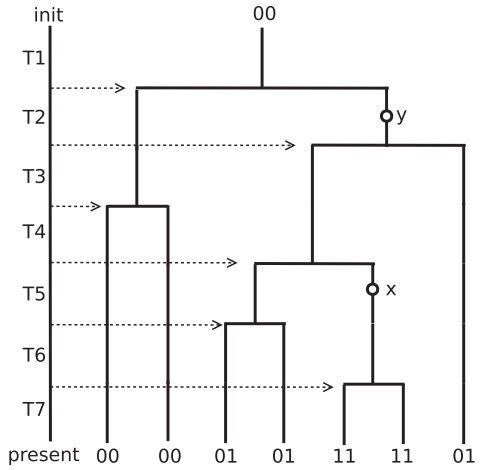
\includegraphics[width=10cm]{chaps/rw/intro_phylo}}
	\caption{عنوانننننننننننننننننننننننن}
	\label{fig:ch_rw:intro_phylo}
\end{figure}

برای استنباط درخت فیلوژنی تومور، الگوریتم کیم وسایمون از سه بخش اصلی تشکیل شده است. طبق قضیه بیز برای محاسبه هر یک از این سه احتمال به مقادیر \gls{likelihood}  نیاز داریم. مقدار احتمال رخداد طبق رابطه¬ زیر محاسبه می¬گردد:

\begin{center}
	\begin{math}
		P(x) = yyyyyyyyyyyyyyyyyyyyyyyyyyyy
	\end{math}
\end{center}

طبق این رابطه و با توجه به اینکه رابطه¬ زمانی میان جهش¬های \lr{x} و \lr{y} دارای 3 حالت 
\begin{center}
	\lr{$x \rightarrow y$} ، \lr{$y \rightarrow x$}  و  \lr{$x \not\leftrightarrow y$}
\end{center}
است، مقدار احتمال محاسبه شده از رابطه فوق به ازای یکی از این سه حالت بیشینه است و به ازای آن حالت یک مسیر جهت¬دار در درخت فیلوژنی قرار خواهد گرفت. طبق آنچه گفته شد یک گرف جهت دار فیلوژنی بلقوه مشابه آنچه در شکل زیر نشان داده ¬شده است استنباط خواهد شد. در نهایت از این گراف جهت دار، یک درخت به طوری که روابط میان جهش¬ها از آن استنباط شود ساخته خواهد شد. 

\begin{figure}[!ht]
	\centerline{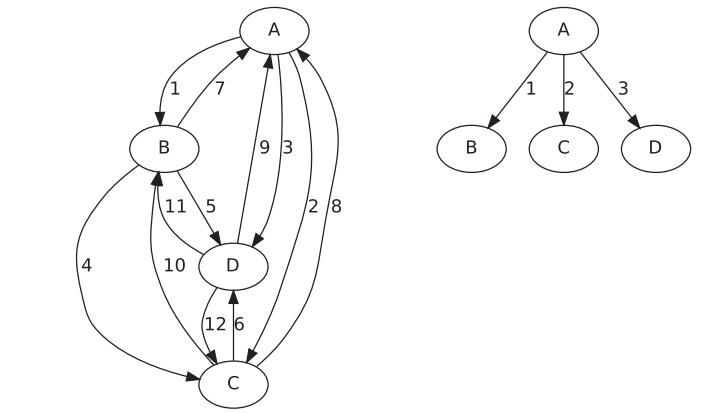
\includegraphics[width=12cm]{chaps/rw/digraph}}
	\caption{عنوانننننننننننننننننننننننننننننننننن}
	\label{fig:ch_rw:digraph}
\end{figure}



در ابتدا یال¬های گرف از طریق رابطه زیر وزن دهی می¬شود:

$-log zzzzzzzzzzzzzzzzzzz$

که در آن \lr{$(x \sim y)$ } رابطه بین جهش¬های \lr{x} و \lr{y} است و \lr{D} نمونه یا سمپل¬های موجود در داده است. بهترین درخت $\hat{T}$  از طریق کمینه¬کردن وزن¬های گراف بدست می¬آید.

\begin{math}
	y=xxxxxxxxxxxxxxxxxxxxxxxxxxx
\end{math}

در شکل بالا محتمل¬ترین \gls{phylogenytree} با بیشینه \gls{likelihood} بر اساس اطلاعات نمونه¬برداری شده بدست می¬آید. در این شکل گراف اولیه و درخت متناظر آن مشاهده می¬شود. مجموع همه وزن¬ها در درخت نهایی با شرط کمینه سازی برابر هفت است که این مقدار کمترین مقدار ممکن است. 


\subsection{پایگاه داده:}

در این مقاله از پایگاه داده تولی¬یابی تک سلولی هو¬ و همکاران \cite{hou2012single} استفاده شده است. این مجموع داده از توالی¬یابی تک¬سلولی \gls{dna} نمونه¬های توموری یک نوع خاص از \gls{thrombocythemia}جمع¬آوری شده است. این مجموعه داده شامل 58 سلول منفرد و 18 نوع جهش یکتا است. اطلاعات کامل در مورد این پایگاه داده از جمله، نام و نوع جهش¬های موجود در دیتابیس، نوع روش نمونه¬برداری و اطلاعاتی دیگر در پایگاه داده \lr{COSMIC} در دسرس عموم قرار دارد. ماتریس ژنوتایپی این پایگاه داده شامل سه مقدار صفر، یک و دو می¬باشد که در آن صفر بیانگر عدم وجود جهش،  یک بیانگر جهش هتروزیگوت و دو نمایانگر جهش هموزیگوت است. یکی از معایب این پایگاه داده نرخ بالای خطای توالی¬یابی تک¬سلولی و بالا¬ بودن نرخ داده¬های از دست رفته (در حدود 45 درصد کل داده¬ها) می¬باشد. همین امر سبب می¬شود تنوع \gls{phylogenytree} نسبت داده شده به این پایگاه داده زیاد باشد. در واقع با در نظر گرفتن حالت¬های مختلف روابط دو¬به¬دوی جهش¬های گوناگون، می¬توان درخت¬های جهشی متنوعی از داده¬ها استنباط کرد. 

\subsection{معیار ارزیابی: }






















		% فصل سوم: روش‌های پیشین
% !TeX root=../../../main.tex

\chapter{روش پیشنهادی}
%\thispagestyle{empty} 
\section{مقدمه} 
%پس از آشنایی با روش‌های پیشین که برای حل مسئله مشابه مورد استفاده قرار گرفته‌اند، حال می‌توانیم به معرفی و تشریح روش‌های پیشنهادی خود برای حل مسئله پیش رو بپردازیم. در این فصل ابتدا داده‌های ورودی مسئله را همراه با فرضیات در نظر گرفته شده بیان می‌کنیم و پس از آن دو روش پیشنهادی متفاوت را بیان خواهیم نمود. در روش اول که به رویکردهای پیشین نزدیک‌تر است با تغییری از جنس روش‌‌های نوین در مراحل میانی به یک روش جدید می‌رسیم که به علت افزایش سرعت همگرایی می‌توان فرض و داده‌های جدیدی را از طریق \gls{cnv} به آن افزود و پاسخ گرفت. اما روش دوم کاملا متفاوت بوده و با رویکردی جدید در حوزه یادگیری ماشین همراه است که به کمک یادگیری تقویتی به حل مسئله مورد نظر می‌پردازد.

پس از آشنایی با روش‌های پیشین که برای حل مسئله مشابه مورد استفاده قرار گرفته‌اند، حال می‌توانیم به معرفی و تشریح روش‌ پیشنهادی خود برای حل مسئله پیش رو بپردازیم. در این فصل ابتدا داده‌های ورودی مسئله را همراه با فرضیات در نظر گرفته شده بیان می‌کنیم و پس از آن روش پیشنهاد خود را بیان خواهیم نمود. این روش با الهام از ۳ روش قبلی متفاوت تنظیم شده است. در ابتدا پایه و بنیان آن به یکی از رویکردهای پیشین نزدیک‌تر است که با تغییری از جنس روش‌‌های نوین در مراحل میانی به یک روش جدید می‌رسیم که به علت افزایش سرعت همگرایی می‌توان فرض و داده‌های جدیدی را از طریق \gls{cnv} به آن افزود و پاسخ گرفت که این عمل با بهره‌گیری از رویکردی جدید در حوزه یادگیری ماشین همراه است که به کمک یادگیری تقویتی به حل مسئله مورد نظر می‌پردازد.

\section{معرفی دادگان ورودی}
قبل از وارد شدن به بخش روش‌های پیشنهادی نیاز است تا دادگان ورودی را مشخص و معرفی نماییم. دادگان ورودی در این پایان‌نامه همگی به صورت فایل‌های خام \gls{ascii} هستند که حاوی اطلاعات جهش‌های ماتریس ژن-سلول (\lr{SNV}) و اطلاعات مربوط به \gls{cnv} هستند.

در ادامه جدول
\ref{tab:ch_pm:firstpmIndices}
را برای معرفی اندیس‌های بکار گرفته شده در روابط مربوط به روش پیشنهادی اول معرفی می‌نماییم.

	\begin{table}[ht]
	\caption{اندیس‌های به کار رفته در روابط روش پیشنهادی}
	\label{tab:ch_pm:firstpmIndices}
	\centering
	\onehalfspacing
	\begin{tabularx}{0.9\textwidth}{|r|X|}
		\hline
		$D$	& ماتریس داده نویزی در دسترس که مقادیر $0$ و $1$ در آن قرار دارد \\
		\hline
		$E$	& ماتریس داده حقیقی بدون نویز که به دنبال آن هستیم \\
		\hline
		$T$	& درخت فیلوژنی جهش‌ها \\
		\hline
		$C$ & پروفایل تعداد کپی نمونه‌ها \\
		\hline
		$\sigma$	 & بردار انتصابات \\
		\hline
		$\wp$ & بردار پذیرش فقدان$  $ \\
		\hline
		$X_T$	& ماتریس متناظر درخت $T$ \\
		\hline
		$N$	& تعداد سلول‌های نمونه \\
		\hline
		$M$	& تعداد جهش‌ها \\
		\hline
		$\mathcal{N}$ & مجموعه سلول‌های متمایز از هم \\
		\hline
		$\mathcal{M}$ & مجموعه جهش‌های متمایز از هم \\
		\hline
		$\mathcal{L}$ & مجموعه جهش‌های با پتانسیل حذف \\
		\hline
		$\alpha$	&  نرخ خطای \gls{falsepositive} \\
		\hline
		$\beta$	& نرخ خطای \gls{falsenegative} \\
		\hline
	\end{tabularx}
\end{table}



\section{روش پیشنهادی برای مدیریت داده‌های از دست رفته}

در ادامه این بخش به معرفی روش‌های پیشنهادی پرداخته خواهد شد اما در ابتدا به دلیل وجود داده‌های از دست رفته در پایگاه‌داده‌های مورد استفاده لازم است تا به بررسی و ارائه رویکردی برای حل این مشکل پرداخته شود و در ادامه پس از معرفی روش پیشنهادی برای مددریت این داده‌های از دست رفته، هر کدام از روش‌های پیشنهادی به تفضیل شرح داده شود.

همان‌گونه که در داده‌های حقیقی مشاهده شد در پایگاه داده‌های حقیقی ما با اطلاعات از دست رفته مواجه هستیم و به همین دلیل نیز سعی کردیم تا در پایگاه داده مجازی تولید شده نیز به مشابه داده‌های حقیقی، شامل اطلاعات از دست رفته باشد. در این بخش به رویکرد روش محاسبه استاتیک برای مدیریت این داده‌های از دست رفته می‌پردازیم و در بخش بعد به معرفی روشی برای بدست آوردن درخت فیلوژنی پرداخته خواهد شد. همان‌گونه که در ادامه بررسی خواهد شد، این اطلاعات از دست رفته در پایگاه داده‌های مختلف نرخ‌های متفاوتی دارد که تاثیر این تغییرات نیز در روشی پیشنهادی بررسی خواهد شد.

\subsection{روش محاسبه استاتیک}
در این روش قصد داریم تا به یک‌باره بتوانیم مقادیر مناسب برای داده‌هایی که از دست رفته‌اند را تخمین بزنیم. در این روش باید توجه شود که ما لزوما به دنبال جایگذاری مقدار از دست رفته با مقدار درست واقعی نیستیم. اگرچه چنین بیانی در نگاه اول ممکن است تعجب‌آور باشد اما با دقت بیشتر متوجه خواهیم شد که ما در آینده برای خطاهای موجود در پایگاه داده مدل‌سازی‌های محدودی داریم. مدل‌هایی که بهترین آن‌ها نیز ممکن است با واقعیت نویز افزوده شده به دادگان متفاوت باشد. در نتیجه اگر مطمئن بودیم که تمام داده‌هایی که موجود می‌باشند بدون خطا هستند در آن صورت ما نیز به دنبال یافتن جایگذاری با مقدار واقعی بودیم اما در حال حاضر که درصدی از داده‌های در دسترس خود همراه با خطا می‌باشند، ما به دنبال جایگذاری‌ای هستیم که بتواند در مجموع با مدل‌سازی خطایی که در نظر می‌گیریم بیشترین سازگاری را داشته باشد کما اینکه ممکن است در حقیقت جایگزاری اشتباهی انجام داده باشیم. حال با توجه به توضیحی که بیان شد به تشریح این روش می‌پردازیم.

با توجه به فرض مدل مکان‌های بی‌نهایت می‌دانیم که جهش‌های اتفاق افتاده در والد در تمامی نسل‌های آینده باقی خواهد ماند. بنابرین اگر تمامی جهش‌های نمونه (سلول) $a$ در نمونه‌ای دیگر مانند $b$ قرار داشته باشد، بنابرین می‌توان نتیجه گرفت که $a$ یکی از اجداد $b$ خواهد بود. همین فرضیه هسته اصلی روش پیشنهادی درنظر گرفته شده را تشکیل می‌دهد. بنابرین اگر جهش $i$ در سلول $a$ از دست رفته است، با توجه به اینکه آن جهش در سلول $b$ چه وضعیتی دارد می‌توان تصمیم‌گیری کرد. اگر $b(i)=0$ باشد، در این صورت $a(i)$ حتما باید $0$ باشد وگرنه فرض اولیه مدل مکان‌های بی‌نهایت نقض خواهد شد. اما اگر $b(i)=1$ باشد، آنگاه نتیجه خاصی نمی‌توان گرفت و باید به دنبال نمونه والد $a$ یعنی نمونه $d$ باشیم. حال اگر $d(i)=1$ باشد، آنگاه $a(i)$ حتما باید $1$ باشد. اما اگر $d(i)=0$ بود آنگاه انتخاب هر مقداری برای $a(i)$ تقریبا آزاد خواهد بود زیرا با فرض اولیه تناقضی ندارد و اینکه ساختار فیلوژنی را تغییر نمی‌دهد. اما از آنجایی که  خود داده‌های در دسترس شامل خطا می‌باشند و هر نمونه‌ای که حاوی اطلاعات از دست رفته است لزوما یک نواده یا یک والد ندارد، مجموعه‌ای از سلول‌های فرزند یا والد خواهند بود که متناسب با پارمترهای خطایی که در نظر می‌گیریم و فاصله ژنی‌ای که دارند می‌توانند در تصمیم‌گیری تاثیرگزار باشند. صورت دقیق‌تر توضیحات داده شده را می‌توان به صورت فرمولی که در ادامه آمده است به نمایش درآورد.
\\
در ابتدا تابعی به نام $F_s(D_{ij})$ تعریف می‌کنیم که به نوعی با توجه به ارزشی که به سلول‌های نواده شده از سلول $j$ می‌دهد سعی دارد تا اطمینان $0$ بودن داده از دست رفته $D_{ij}$ را بیان کند.
\\
برای محاسبه این تابع می‌دانیم که ابتدا سلول‌های مختلف با توجه به احتمال نواده بودنشان باید رتبه‌بندی شوند و وزن بگیرند. پس از آن  هر سلول متناسب با ارزش تاثیرگزاری خود می‌تواند در مورد جایگاه جهش $i$ برای سلول $j$ نظر دهد.
\begin{equation}
	F_s(D_{ij}) = \sum_{n \in \mathcal{N}}  (1-D_{mj})  \prod_{m=1}^{M} W(D_{mn}, D_{mj})
	\label{eq:ch_pm:F_s_simple}
\end{equation}

در فرمول \ref{eq:ch_pm:F_s_simple} مجموعه $\mathcal{N}$ برابر با مجموعه سلول‌های متمایز از هم است. زیرا که در بسیاری از پایگاه‌داده‌ها از یک نمونه سلول ممکن است چندین نمونه وجود داشته باشد که وجود آن‌ها باعث بایس در محاسبات ما خواهد شد. همچنین تابع $W_s(c,p)$ به ارزش‌دهی جهش $c$ در برابر $p$ به عنوان نواده بودن می‌پردازد که در فرمول \ref{eq:ch_pm:W_simple} تعریف شده است.
\begin{equation}
	W(c, p) = 
	\begin{cases}
		1 	       &\qquad \text{\lr{if}} \quad c=1, p=1 \\
		1-\xi   &\qquad \text{\lr{if}} \quad c=1, p=0 \\
		0 		  &\qquad \text{\lr{if}} \quad c=0, p=1 \\
		1 	 	  &\qquad \text{\lr{if}} \quad c=0, p=0
	\end{cases}
	\label{eq:ch_pm:W_simple}
\end{equation}
مقدار $\xi$ عددی بین $(0,1)$ است که پارامتری در جهت میزان ارزش‌دهی به نوادگان با فواصل مختلف می‌باشد. هرچه این عدد بزرگتر باشد به معنی کم‌ارزش‌تر شدن نوادگان با فواصل بیشتر است و بلاعکس.
\\
به همین صورت برای اولاد سلول $j$ نیز می‌توان مشابه حالت قبل عمل کرد که روابط آن به صورت فرمول‌ \ref{eq:ch_pm:F_a_simple} خواهد شد.
\begin{equation}
	F_a(D_{ij}) = \sum_{n \in \mathcal{N}}  D_{mj}  \prod_{m=1}^{M} W(D_{mj}, D_{mn})
	\label{eq:ch_pm:F_a_simple}
\end{equation}
حال دو نکته در استفاده از روابط بالا باقی خواهد ماند. 
\\
نکته اول وجود داده‌های دیگر از دست رفته در محاسبه توابع است که به دو صورت می‌توان با آن‌ها برخورد  نمود. رویکرد اول این است که در آن‌جایگاه ژنی از محاسبه آن خود داری شود و رویکرد دوم استفاده از از مقدار $0.5$ یا فراوانی نسبی آن جهش در محسبات است که ما رویکرد اول را در این گزارش استفاده خواهیم کرد.
\\
نکته دوم وجود خطا در داده‌هاست. برای مدیریت این مشکل می‌توان با مدل‌سازی خطا که به صورت فرمول \ref{eq:ch_pm:P_alpha_beta} بیان می‌شود، برخورد کرد.
\begin{equation}
	\begin{aligned}
		&P(D_{ij}=1|E_{ij}=0)=\alpha, &\qquad P(D_{ij}=0|E_{ij}=0)=1-\alpha \\ &P(D_{ij}=0|E_{ij}=1)=\beta, &\qquad P(D_{ij}=1|E_{ij}=1)=1-\beta
	\end{aligned}
	\label{eq:ch_pm:P_alpha_beta}
\end{equation}
پس از تعریف مدل‌سازی خطا می‌توان روابط قبلی را مجددا به صورتی که در ادامه آمده است بازنویسی کرد.
\begin{equation}
	\begin{aligned}
		W_e(c,p) = \sum_{i,j \in \{0,1\}} P(c|E_c=i)P(p|E_p=j)W(i,j)
	\end{aligned}
	\label{eq:ch_pm:W_e}
\end{equation}
که در این صورت توابع $F_p$ و $F_a$ نیز به صورت زیر همراه با مدل‌سازی خطا بازتعریف خواهند شد.
\begin{equation}
	\begin{aligned}
		\hat{F}_s(D_{ij}) &= \sum_{n \in \mathcal{N}}  [1-D_{mj}(1-\alpha)]  \prod_{m=1}^{M} W_e(D_{mn}, D_{mj}) \\
		\hat{F}_a(D_{ij}) &= \sum_{n \in \mathcal{N}}  D_{mj}(1-\beta)  \prod_{m=1}^{M} W_e(D_{mj}, D_{mn})
	\end{aligned}
	\label{eq:ch_pm:F_all_final}
\end{equation}
حال پس از محاسبه مقادیر $\hat{F}_s$ و $\hat{F}_a$ می‌توان در مورد داده نامعلوم $D_{ij}$  به صورت فرمول \ref{eq:ch_pm:F_to_D} تصمیم گرفت.
\begin{equation}
	D_{ij} = \begin{cases}
		0 \qquad \text{\lr{if}} \quad \hat{F}_s \ge \hat{F}_a \\
		1 \qquad \text{\lr{if}} \quad \hat{F}_s < \hat{F}_a
	\end{cases}
	\label{eq:ch_pm:F_to_D}
\end{equation}
همچنین با کمی دقت در فرمول‌بندی انجام شده اگر برای تمام $i,j$های ماتریس $D$ این مقادیر توابع $\hat{F}$ محاسبه شوند، خود می‌توانند معیاری برای ارزیابی پایگاه‌داده در دسترس و احتمال درستی فرض مدل مکان‌های بی‌نهایت باشند.

%	\subsection{روش بیشینه درست‌نمایی}
%	در این روش هر کدام از جهش‌های نامشخص و از دست رفته با توجه به بیشینه شدن درست‌نمایی مشخص خواهند شد. در واقع در این رویکرد به دو صورت می‌تواند انجام شود. نخست آنکه برحسب یک مدل از پیش تعریف‌شده،


\subsection{تصادفی}
پر کردن کاملا تصادفی میس‌ها. در این روش به صورت تصادفی مقادیر از دست رفته را مقدار دهی می‌کنیم. تنها نکته‌ای که در این روش وجود دارد این است که نباید این پرکردن تصادفی داده‌های از دست رفته باعث شود تا پارامترهای مدل‌سازی‌ای که از قبل در نظر گرفته بودیم با این روش نادقیق شوند.


	
	

\section{روش پیشنهادی}
در این روش ما بر حسب بهتر کردن یک پاسخی که از پیش داشتیم به دنبال رسیدن به بهترین پاسخ ممکن در طی \glspl{iteration} 
پشت سر هم هستیم. 
%برای مشخص شدن نحوه کارکرد روش پیشنهادی در مراحلی که در ادامه بیان خواهد شد به عنوان مثال یک ماتریس 
%\begin{equation}
%	D=\left[
%	\begin{array}{cccc}
%		0 & 1 & 1 & 0 \\ 
%		0 & 0 & 1 & 1 \\ 
%		1 & 0 & 1 & 0 \\ 
%		1 & 1 & 0 & 1 \\ 
%		1 & 0 & 1 & 1 \\ 
%		0 & 1 & 1 & 1
%	\end{array} 
%	\right]
%	\label{eq:ch_pm:pm1_ex_D}
%\end{equation}
% را به عنوان ورودی مساله به همراه پارامترهای $\alpha$ و $\beta$ در نظر بگیرید. (برای راحتی کار فرض کرده‌ایم که داده از دست رفته در $D$ نداریم.)

\subsection{پیش‌پردازش}
قبل از شروع باید بر روی داده‌ها یک پیش‌پردازش اعمال کنیم که وابسته به سیاست درنظر گفته شده می‌تواند باعث تغییر در پاسخ نهایی نیز شود. به این منظور داده‌هایی که \lr{miss} شده‌اند با یکی از دو روشی که معرفی شد تخمین رده می‌شوند و برای ورود به مرحله بعد آماده می‌شوند.

\subsection{اولین پاسخ (درخت تصادفی)}
همان‌گونه که از قبل می‌دانستیم خروجی نهایی ما برابر با درختی خواهد بود که نودهای آن برابر با جهش‌های ماتریس ورودی ما و برگ‌های آن برابر با نمونه‌های مشاهده شده خواهند بود. در روش پیشنهادی اول ما به دنبال بهتر کردن این درخت به عنوان پاسخ هستیم. از این رو پایه این روش پیشنهادی اول بر مبنای بهتر کردن پاسخ فعلی بنا نهاده شده است. در نتیجه ما همواره پاسخی به عنوان جواب نهایی داریم که تلاش خواهیم نمود تا با استفاده از ابزرهایی بتوانیم ابا ایجاد تغییری در این پاسخ به پاسخی جدید برسیم که قابل مقایسه با پاسخ فعلی برای انجام مراحل بعدی باشد.
\\
 با توجه به توضیحاتی که داده شد ما برای شروع الگوریتم پیشنهادی اول خود نیاز به یک پاسخ داریم. این پاسخ که درخت فیلوژنی هست با توجه پارامترهای ورودی و انتخاب یک نود (ژن) $root$ به عنوان ریشه این درخت به صورت زیر حاصل می‌شود.
 \begin{equation}
 	\begin{aligned}
 		\mathcal{M} &= \{1\dots M\} \\
 		\hat{B}_{T_1} &= [R_1(\mathcal{M}-|1|), R_2(\mathcal{M}-|2|), \dots, R_{root}(\{\}), \dots, R_M(\mathcal{M}-|M|)] 
 	\end{aligned}
 \end{equation}
که در این رابطه $\mathcal{M}$ برابر با مجموعه تمامی جهش‌های متمایز از شماره $1$ تا  $M$ است و $\hat{B}$ مشخص‌کننده نود پدر در درخت برای جهش $i$ام در این لیست خود است که توسط تابع $R_i(X)$ به صورت کاملا \gls{uniform} از اعضای مجموعه  $X$ انتخاب می‌شود.
\\
% با توجه به مثالی که در رابطه \ref{eq:ch_pm:pm1_ex_D} زده شد فرض کنید مقدار بردار $\hat{B}$ با ریشه $root=2$ به صورت رابطه \ref{eq:ch_pm:pm1_ex_B} شود.
%\begin{equation}
%	\hat{B} = [2, 1, -, 0]
%	\label{eq:ch_pm:pm1_ex_B}
%\end{equation}
%که درخت شکل \ref{fig:ch_pm:pm1_T1} را نتیجه می‌دهد.
%\begin{figure}[!ht]
%	\centering 
%%	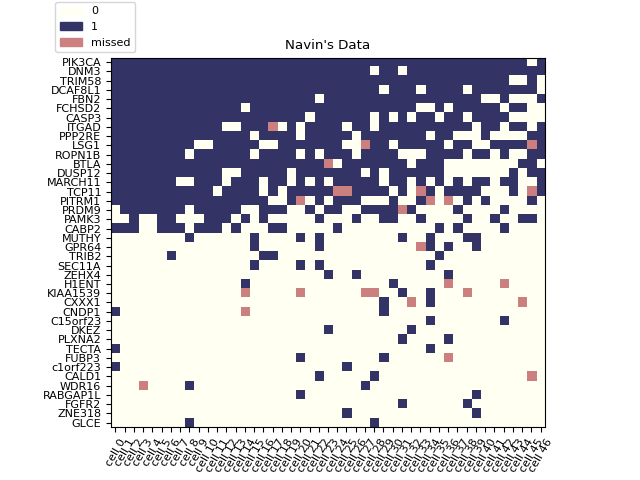
\includegraphics[width=0.67\textwidth]{img/dataset/r/Navin_Dm.png}
%	\caption{درخت تصادفی اول}    
%	\label{fig:ch_pm:pm1_T1}
%\end{figure}

\subsection{پاسخی جدید}
تا به اینجا ما یک درخت فیلوژنی به عنوان پاسخ داریم که در این بخش می‌خواهیم با انجام تغییراتی بر روی آن به یک پاسخ جدید برسیم تا در گام‌های بعدی بتوانیم با مقایسه آن‌ها تصمیمات لازم را برای ادامه الگوریتم بگیریم. به همین منظور تقریبا مشابه با روش \cite{davis2016computing} به صورت \gls{pruneandreattach} قصد داریم تا درخت پاسخ فعلی را برای رسیدن به یک پاسخ دیگر تغییر دهیم. 
\begin{figure}[!ht]
	\centering 
	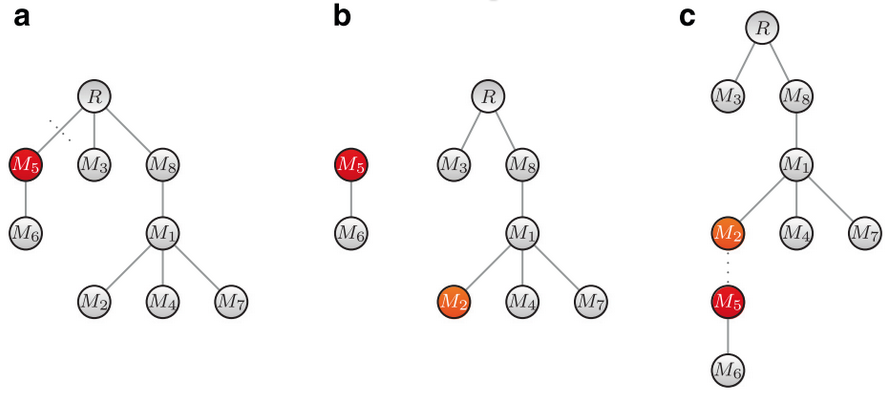
\includegraphics[width=0.9\textwidth]{img/chaps/pm/pruneandreattach}
	\caption{نحوه انجام کار روش \gls{pruneandreattach} \cite{davis2016computing}.}    
	\label{fig:ch_pm:pruneandreattach}
\end{figure}
در شکل \ref{fig:ch_pm:pruneandreattach} مثالی از این روش آورده شده است. در این شکل مطابق با قسمت \lr{a} یکی از نودهای درخت (به جز ریشه) انتخاب می‌شود (در اینجا نود \lr{$M_5$}) و اتصال از پدرش قطع می‌شود. در این حالت به دو درخت مشابه با شکل \lr{b} می‌رسیم. حال در درخت باقی مانده یک نود دیگر  (\lr{$M_2$}) به عنوان پدری جدید انتخاب می‌شود تا با این تغییر به درخت جدید شکل \lr{c} برسیم.
\\
در نتیجه با این تکنیک می‌توان به پاسخ‌های جدید رسید اما سوالی که باقی ماند این است که این دو نود چگونه باید انتخاب شوند؟ 
این دو انتخاب به صورت هوشمند با استفاده از خروجی یک شبکه عمیق گرفته می‌شود. این شبکه که در اصل در دسته شبکه‌های \gls{reinforcementlearning} عمیق است، از پیش برای این منظور آموزش داده شده‌ است.
%\begin{equation}
%	\begin{aligned}
%		
%	\end{aligned}
%	T_{}
%	T_{i+1} = \text{Attach}(T_{i}, )
%\end{equation}
شبکه مورد نظر برای انتخاب محل برش (هرس) و مکان مناسب برای بازاتصال را ارزش‌گزاری می‌کند. ساختار این شبکه در قسمت \ref{sec:ch_pm:network} به تفضیل شرح داده شده است.

\subsection{مقایسه و ارزیابی پاسخ‌ها}
پس از اینکه از پاسخ فعلی به یک پاسخ جدید رسیدیم حال می‌توان کیفیت این دو پاسخ را باهم مقایسه کرد و پس از آن با توجه به امتیاز دو پاسخ در مورد پذیرش یا عدم پذیرش پاسخ جدید در برابر پاسخ فعلی تصمیم گرفت. این فرآیند شامل دو بخش اصلی است که در دو زیربخشی که در ادامه آمده است بیان شده‌اند.

\subsubsection{تبدیل درخت پاسخ به ماتریس}
برای ادامه روش پیشنهادی و مقایسات لازم است تا درخت پاسخ را به ماتریس $X$ تبدیل کنیم که قابل بررسی با داده‌های مشاهده شده $D$ باشد. ماتریس $X$ مشابه با ماتریس  $D$ متشکل از مقادیر $0$ و $1$ خواهد بود که به عنوان مثال $X_{i,j}=1$ به این معنی است که طبق درخت $T$ در سلول $i$ جهش $j$ مشاهده نشده است.
ما هر درخت $T$ را می‌توانیم با مقادیر مختلفی از $\sigma$ و $\wp$ مزین کنیم و به ماتریس‌های مختلفی برسیم. اما در نهایت مهمترین پارامترها که بیشترین امتیاز را برای درخت ما بوجود می‌آورند مطلوب ما خواهند بود و ماتریس متناظر با آن حالت را $X$ می‌نامیم و به مراحل بعدی برای محاسبات انتقال می‌دهیم.
در نتیجه کار ما در این بخش این خواهد بود که به ازای درخت دلخواه $T$ بتوانیم بهترین $\sigma$ و $\wp$ را بدست آوریم و از روی آن‌ها ماتریس متناظر $X$ را بدست آوریم.
از پیش با بررسی \glspl{cnp} در بخش 	\ref{sec:ch_pm:L} به $\mathcal{L}$ رسیده‌ایم که مشخص می‌کند چه جهش‌هایی پتانسیل حذف را دارند و در این بخش زمان استفاده از این اطلاعات است.
در ادامه ماتریس $B$ را به صورت رابطه \ref{eq:ch_pm:iB} تعریف می‌کنیم که برای انتخاب بهینه $\sigma$ مورد استفاده قرار خواهد گرفت.
 \begin{equation}
	B_{i,j} = 
	\begin{cases}
		1 		  &\qquad \text{\lr{if}} \quad \text{$i=j$ یا $i$ یکی از نوادگان $j$ باشد که در $\mathcal{L}$ نباشد} \\
		x 	 	  &\qquad \text{\lr{if}} \quad \text{$i$ یکی از نوادگان $j$ باشد و همچنین در $\mathcal{L}$ باشد} \\
		0 	       &\qquad \text{\lr{if}} \quad \text{در صورتی که دو مورد بالایی نباشد}
	\end{cases}
	\label{eq:ch_pm:iB}
\end{equation}
در رابطه بیان شده $x$ به معنای این است که هم می‌تواند مقدار $0$ و هم مقدار $1$ را داشته باشد.\\
حال می‌توانیم برای هر سلول (نمونه) $c_i$ در ماتریس مشاهده شده $D$ امتیاز اتصال را در هر قسمت از درخت $T$ حساب می‌کنیم که از طریق رابطه \ref{eq:ch_pm:score_B} بدست می‌آید.
\begin{equation}
	S(c_i, T, k) = \prod_{j=0}^{M}P(D_{i,j}|B_{j,k}) 
	\label{eq:ch_pm:score_B}
\end{equation}
در این رابطه $S(c_i, T, k)$ برابر امتیاز اتصال نمونه $i$ در درخت $T$ در مکان ژن (جهش) $k$ است.
ناگفته نماند که،
\begin{equation}
	P(D=1|B =x) = 1-\beta, \qquad P(D=0|B=x) = 1-\alpha
	\label{eq:ch_pm:score_p_x}
\end{equation}
بنابرین به ازای هر $x$ ما دو حالت را می‌توانیم داشته باشیم که آن‌ها همان پذیرش یا عدم پذیرش حذف جهش‌های در مجموعه $\mathcal{L}$ است. برای اینکه بهترین $\wp$ را داشته باشیم باید بتوانیم این امتیازاتی که با پذیرش‌های مختلف $x$ بدست می‌آیند را به ازای تمام نمونه‌های در دسترس ثبت و بررسی کنیم.
برای این منظور رابطه \ref{eq:ch_pm:iB} را به صورت رابطه \ref{eq:ch_pm:B} بازنویسی می‌کنیم.
 \begin{equation}
	B_{i,j} = 
	\begin{cases}
		1 		  &\qquad \text{\lr{if}} \quad \text{اگر $i$ یکی از نوادگان $j$ باشد که در $\mathcal{L}$ نباشد} \\
		x_{i}^{\text{\lr{dist($i$,$j$)}}} &\qquad \text{\lr{if}} \quad \text{اگر $i$ یکی از نوادگان $j$ باشد و همچنین در $\mathcal{L}$ باشد} \\
		0 	       &\qquad \text{\lr{if}} \quad \text{در صورتی که دو مورد قبلی نباشد}
	\end{cases}
	\label{eq:ch_pm:B}
\end{equation}
همان‌گونه که در این رابطه بیان شده همچنان مقادیر نامشخص وجود دارد. برای مشخص کردن این مقادیر نامشخص از $\wp$ استفاده می‌کنیم. $\wp$ یک لیست به طول تعداد ژن‌هایی است که در مجموعه $\mathcal{L}$ قرار دارند. نتیجه اعمال $\wp$ بر  $B$ ماتریس $A$ را نتیجه خواهد داد که به صورت زیر تعریف می‌شود.
\begin{equation}
	A_{i,j} = 
	\begin{cases}
		1 &\qquad \text{\lr{if}} \quad \text{$B_{i,j}=1$ یا $\wp_i<\text{\lr{dist($i$,$j$)}}$} \\
		0 &\qquad \text{\lr{if}} \quad \text{شرط بالا درست نباشد}
	\end{cases}
	\label{eq:ch_pm:A}
\end{equation}
این مقادیر نامشخص که در اتصال به ژن $i$ و نوادگان آن در درخت مشخص شده‌اند با توجه به فاصله تعیین شده از این ژن $i$ برای نوادگان حذف خواهد شد که این فاصله در $\wp_i$ مشخص شده است. پس حال با تعیین مقادیر بردار $\wp$ می‌توانیم بهترین $B$ نامعلوم را به $A$ معلوم تبدیل کنیم.
به رابطه \ref{eq:ch_pm:score_B} توجه کنید. این رابطه امتیاز اتصال نمونه $i$ را به مکان $k$ در درخت بیان می‌کند. ما به دنبال محلی هستیم که ضمیمه کردن نمونه به آن محل بالاترین امتیاز را بدست آورد. بنابرین $\sigma$ را به صورت یک بردار به طول $N$ (تعداد نمونه‌ها) تعریف می‌کنیم به طوری که شماره اندیس $i$ در آن متناظر با $i$امین نمونه در ماتریس $D$ باشد و مقداری که در آن خانه از $\sigma$ قرار می‌گیرد برابر با شماره یکی از ستون‌های ماتریس $A$ باشد که نشان‌دهنده بهترین محلی است که در درخت $T$ می‌تواند به آن ضمیمه شود.
حال می‌توانیم جایگاه هر اتصال به درخت را که بالاترین امتیاز را به ارمغان می‌آورد مشخص کنیم و پس از آن به تبدیل درخت $T$ به ماتریس $X$ بپردازیم.
\begin{equation}
	\begin{aligned}
		S(c_i, T) &= \max_{k \in \{0 \dots M\}} S(c_i, T, k) \\
		&= \max_{j^*} \left( \prod_{k=0}^{M}P(D_{i,k}|A_{k,j^*})\right) = S(c_i, T, \sigma_i)
	\end{aligned}
	\label{eq:ch_pm:score_attach}
\end{equation}
رابطه \ref{eq:ch_pm:score_attach} همان‌طور که مشاهده می‌شود به راحتی قابل حل می‌باشد و نمونه‌ها مستقل از هم هستند و می‌توانند به درخت اتصال یابند اما ما تا به اینجا بهترین $\sigma$ را به ازای یک $\wp$ یافته‌ایم. آیا مقدار $\wp$ نیز بهینه است؟
برای مشخص کردن مقدار بهینه $\wp$ برای درخت دلخواه $T$ از رابطه‌ای که در ادامه آمده است کمک می‌گیریم.
\begin{equation}
	\langle\hat{\wp}, \hat{\sigma}\rangle = \arg \max_{\wp, \sigma} \prod_{i=1}^{N}S(c_i, T)
	\label{eq:ch_pm:T_score}
\end{equation}
در واقع این مقادیر $\wp$ باید به گونه‌ای انتخاب شوند تا مجموع امتیازات همه اتصالات به درخت در حالت بیشینه خود باشد که برابر با امتیاز درخت می‌شود که در این حالت به $\hat{\wp}$ می‌رسیم که ماتریس $A$ حاصل از آن را $\hat{A}$ می‌نامیم. در نهایت که بهترین مقادیر به ازای درخت مشخص شدند پس می‌توان $X$ را به صورت رابطه \ref{eq:ch_pm:X} تشکیل داد.
\begin{equation}
	X_{i,j} = \hat{A}_{i, \hat{\sigma}_{j}}
	\label{eq:ch_pm:X}
\end{equation}



\subsection{یافتن جهش‌های با پتانسیل حذف}
\label{sec:ch_pm:L}

همان‌گونه که از ابتدا می‌دانیم ما به دنبال درخت فیلوژنی حقیقی داده‌های نویزی مشاهده شده $D$ هستیم. این درخت در این روش برابر با درختی است که،
\begin{itemize}
	\item نحوه قرارگیری ژن‌ها در ساختار درخت ($T$)
	\item محل‌هایی در درخت که جهش‌های قبلی در آن‌ها حذف می‌شوند ($\wp$)
	\item نحوه انتصاب نمونه‌های مشاهده شده به درخت ($\sigma$)
	\item و در نهایت پارامترهایی که برای مدل‌سازی خطای بوجود آمده در داده‌های در دسترس‌مان تعیین شده است ($\theta$)
\end{itemize}
به گونه‌ای انتخاب شوند که محتمل‌ترین حالت را برای مشاهده داده‌های $D$ بوجود آورند که در این حالت ما رابطه 
علت توضیحات مجدد این موارد به این دلیل است که یکی از تفاوت‌های مهم با روش‌های مشابه گذشته در همین بخش و نحوه استفاده از داده‌های \gls{cnv} است. این مرحله در هر \gls{iteration} باید انجام شود و متناسب با درختی که در اختیار داریم نمونه‌ها و پروفایل تکرارها را بررسی کنیم تا در ساختار آن درخت بتوانیم تقریبی بیابیم که کدام نمونه‌ها به ژن‌های پایین‌تر و کدام بالاتر منتصب می‌شوند تا پس از آن پروفایلشان را بنگریم که آیا تعداد تکرارها کاهشی است یا افزایشی که بتوانیم لیست $\mathcal{L}$ را بسازیم.
\\
با توجه به توضیحات داده شده هر \gls{gene} $i$ را در درخت فعلی $T$ انتخاب می‌کنیم. پس از آن طبق رابطه \ref{eq:ch_pm:L_pre} ما سه دسته از ژن‌ها را به ازای \gls{gene} در درخت $T$ خواهیم داشت.
\begin{equation}
	\begin{aligned}
		Pa(T, i) &= \{g| g \in T, g \in \text{\lr{path($i$, $root$)}}\}\\
		Ch(T, i) &=\{g| g \in T, i\in \text{\lr{path($g$, $root$)}}\}\\
		Br(T, i) &= \{g| g \in T, g \not\in (Pa(T, i) \cup Pa(T, i))\}
	\end{aligned}
	\label{eq:ch_pm:L_pre}
\end{equation}

این سه دسته برابر با دسته اجداد \gls{gene} $i$ به نام $Pa(T, i)$، دسته نوادگان \gls{gene} $i$ به نام $Ch(T, i)$ و در نهایت دسته برادران \gls{gene} $i$ به نام $Br(T, i)$ در $T$ می‌باشند.
حال از پس مشخص کردن این دسته‌ها با انتصاب نمونه‌ها به آن‌ها می‌توان امتیازی را به عنوان پتانسیل قابلیت حذف \gls{gene} $i$ در درخت فعلی $T$ محاسبه کرد.
این نحوه انتصاب نمونه‌ها به گروه‌ها از طریق رابطه \ref{eq:ch_pm:G_set_score} انجام می‌شود.
\begin{equation}
	\begin{aligned}
		S_{Pa}(x, \theta) &= \left(\prod_{j\in Pa}P(x_j|1)\right) \times\left(\prod_{j\in Ch}P(x_j|0)\right) \times\left(\prod_{j\in Br}P(x_j|0)\right)\\
		S_{Ch}(x,, \theta) &=\left(\prod_{j\in Pa}P(x_j|1)\right) \times\left(\prod_{j\in Ch}P(x_j|1)\right) \times\left(\prod_{j\in Br}P(x_j|0)\right)\\
		S_{Br}(x,, \theta) &= \left(\prod_{j\in Pa}P(x_j|1)\right) \times\left(\prod_{j\in Ch}P(x_j|0)\right) \times\left(\prod_{j\in Br}P(x_j|1)\right)
	\end{aligned}
	\label{eq:ch_pm:G_set_score}
\end{equation}

در این رابطه همانطور که مشخص است به ازای هر نمونه یک امتیاز به منظور متعلق بودن به دسته‌های تعریفی رابطه \ref{eq:ch_pm:L_pre} بدست می‌آید. پس از این مرحله کافی است تا طبق رابطه \ref{eq:ch_pm:L_score} نمونه‌هایی که در گروه $Ch(T, i)$ قرار گرفته‌اند را برمی‌گزینیم و بقیه را کنار می‌گزاریم. پس از آن \glspl{gene}یی که در این گروه قرار گرفته‌اند را به عنوان زیر درختی جدید به ریشه $i$ در نظر می‌گیریم و برای تمامی نودهای آن این گروه‌ها را مجددا تشکیل می‌دهیم. حال باید در این زیر درخت تغییرات تعداد کپی را در محل قرارگیری \gls{gene} بررسی کنیم که آیا کاهشی است یا افزایشی و به این تغییرات امتیاز دهیم و با توجه به امتیازهای کسب شده و آستانه‌گزاری برای آن‌ها تصمیم‌گیری می‌کنیم که در مجموعه $\mathcal{L}$ قرار می‌گیرند یا خیر.
\begin{equation}
	DPS(T, i) = \frac{1}{N}\sum_{p\in Pa, c\in Ch} \left( \max\left( {0, C_c^i-C_p^i}\right)  \ln\frac{S_{Pa}(p)}{S_{Ch}(c)} \right)
	\label{eq:ch_pm:L_score}
\end{equation}
اگر تغییرات در بین نمونه‌ها به نحوی بود که مشاهداتی از کاهش تعداد کپی از گروه اجداد زیردرخت به نوادگان زیردرخت بود در آن‌صورت به ازای هر مشاهده متناسب با قدرت مشاهده که از میزان فاصله تغییرات و نزدیکی نمونه‌ها به محل \gls{gene} در درخت نشات می‌گیرد، به امتیاز \gls{gene} $i$ اضافه می‌کنیم و در غیر این صورت هیچ. در نهایت امتیاز بدست آمده را بر تعداد کل مشاهدات تقسیم می‌کنیم که امتیاز نهایی برای این \gls{gene} در این درخت $T$ با توجه به نمونه‌های در دسترس بدست می‌آید.
\\
در بخش‌های دیگر نحوه استفاده از این لیست $\mathcal{L}$ برای ادامه علمیات و ارزش‌گذاری درخت به تفضیل شرح داده شده است.


\subsubsection{مقایسه پاسخ فعلی با پاسخ آرمانی}
پس از استخراج ماتریس مناسب از درخت می‌توان به ارزش‌گزاری و محاسبه \gls{likelihood} پرداخت. این عمل به صورت رابطه \ref{eq:ch_pm:pm1_likelihood} محاسبه می‌شود. 

\begin{equation}
	L: P(D|T,\sigma, \wp, \theta) = \prod_{n=1}^{n=N}\prod_{m=1}^{m=M}P(D_{nm}|X_{nm})
	\label{eq:ch_pm:pm1_likelihood}
\end{equation}
که $X$ برابر ماتریس بدست آمده از درخت $T$ با توجه به بردارهای $\sigma$ و $\wp$ است. این رابطه بیانگر احتمال مشاهده ماتریس داده ورودی $D$ در صورتی است که درخت فیلوژنی صحیح $T$ و پارامترهای حقیقی $\theta$ باشد که توسط بردارهای $\sigma$ و $\wp$ تثبیت شده است. هرچه این احتمال بالاتر باشد نمایانگر این است که درخت، پارامترها و بردارهای کنترلی ما بگونه‌ای انتخاب شده‌اند که محتمل‌ترین حالت برای مشاهده داده‌های ورودی ما هست و در این صورت بهترین پاسخ برای ما همان پاسخی خواهد بود که محتمل‌ترین باشد. از این رو با دانستن $\theta$ ما به دنبال $T$ای به همراه بردارهای مربوطه آن هستیم که پاسخ رابطه \label{eq:ch_pm:pm1_maxML} باشد.
\begin{equation}
	(T, \sigma, \wp)_{\text{\lr{ML}}} = \arg\max_{(T, \sigma, \wp)} P(D|T,\sigma, \wp, \theta)
	\label{eq:ch_pm:pm1_maxML}
\end{equation}
 اما همانگونه که می‌دانیم ما به دنبال بهترین درخت $T$ هستیم که $\sigma$ و $\wp$ در آن درخت برای ما اهمیت دارند. در واقع هر درخت $T$ دارای امتیاز $S(T)$ است که به صورت رابطه \label{eq:ch_pm:pm1_sT} تعریف می‌شود.
 \begin{equation}
 	S(T) = P(D|T,\sigma^*, \wp^*)
% 	, \qquad \sigma^*=\arg\max_{\sigma}P(D|T,\sigma, \wp)
 	\label{eq:ch_pm:pm1_sT}
 \end{equation}

\subsection{پذیرش پاسخ‌های جدید و یافتن بهترین پاسخ}
در این مرحله ما دو پاسخ با امتیازهایشان در اختیار داریم که می‌توانیم برحسب آن‌ها برای ورود به \gls{iteration} بعد تصمیم‌گیری نماییم. این فرآیند توسط رابطه‌ای که در ادامه آمده است انجام می‌شود.
\begin{eqnarray}
	p_{\text{acc}} = \min\Bigg[1, \left(\frac{P(E=X_{i+1}|D, \theta)}{P(E=X_{i}|D, \theta)}\right)^{\rho^{-1}}\Bigg]
	 \label{eq:ch_pm:pm1_accepting} 
\end{eqnarray}
در رابطه \ref{eq:ch_pm:pm1_accepting}، اگر پاسخ جدید بهتر از پاسخ فعلی باشد بیان می‌کند که افزایش بهینگی در پاسخ جدید باعث می‌شود تا صورت کسر مقداری بیش از مخرج بگیرید که در این صورت $p_{\text{acc}}$ که برابر با احتمال پذیرش پاسخ جدید است، برابر $1$ خواهد شد که یعنی حتما پاسخ جدید به عنوان پاسخ پابرجا برای ورود به \gls{iteration} بعد در نظر گرفته می‌شود. اما اگر پاسخ جدید (درخت جدید) بهتر از پاسخ فعلی ارزیابی نشود ما آن را مستقیما رد نمی‌کنیم و به احتمالی کمتر از $1$ ممکن است آن را بپذیریم. دلیل این پذیرش جلوگیری از به دام افتادن الگوریتم در پاسخ‌مان در \gls{localmaxima} است. در شکل \label{fig:ch_pm:pm1_rho} تاثیر تغییر پارامتر $\rho$ در احتمال پذیرش پاسخ‌های جدیدی که مطلوب‌تر از پاسخ فعلی نیستند نمایش داده شده است.
\begin{figure}
	\centering
	\begin{tikzpicture}
		\begin{axis}[xmin = 0, xmax = 1, ymin = 0, ymax = 1,
			xtick distance = 0.1, ytick distance = 0.1, grid = both, minor tick num = 1,
			major grid style = {lightgray!50}, minor grid style = {lightgray!25},
			width = 0.8\textwidth, height = 0.55\textwidth,
			xlabel = {$x=\frac{P(E=X_{i+1}|D, \theta)}{P(E=X_{i}|D, \theta)}$}, ylabel = {$f(x)=p_\text{acc}$},
			legend style={at={(1.01,1.015)}, draw=none, anchor=north west}]
			% Plot a function
			\addplot[domain = 0:1,samples = 1000,smooth,thick,Orchid,] {x^(3^-1)};
			\addplot[domain = 0:1,samples = 1000,smooth,thick,violet,] {x^(2^-1)};
			\addplot[domain = 0:1,samples = 1000,smooth,thick,Turquoise,] {x^(1.5^-1)};
			\addplot[domain = 0:1,samples = 1000,smooth,thick,Silver,] {x^(1.25^-1)};
			\addplot[domain = 0:1,samples = 100 ,smooth,thick,Salmon,] {x^(1.0^-1)};
			\addplot[domain = 0:1,samples = 100 ,smooth,thick,blue,] {x^(0.9^-1)};
			\addplot[domain = 0:1,samples = 100 ,smooth,thick,red,] {x^(0.8^-1)};
			\addplot[domain = 0:1,samples = 100 ,smooth,thick,brown,] {x^(0.7^-1)};
			\addplot[domain = 0:1,samples = 100 ,smooth,thick,black,] {x^(0.6^-1)};
			\addplot[domain = 0:1,samples = 100 ,smooth,thick,cyan,] {x^(0.5^-1)};
			\addplot[domain = 0:1,samples = 1000,smooth,thick,green,] {x^(0.4^-1)};
			\addplot[domain = 0:1,samples = 1000,smooth,thick,pink,] {x^(0.3^-1)};
			\addplot[domain = 0:1,samples = 1000,smooth,thick,magenta,] {x^(0.2^-1)};
			\addplot[domain = 0:1,samples = 1000,smooth,thick,teal,] {x^(0.1^-1)};
			% Legend
			\legend{$\rho=3.0$,$\rho=2.0$,$\rho=1.5$,$\rho=1.25$,$\rho=1.0$,$\rho=0.9$,$\rho=0.8$,$\rho=0.7$,$\rho=0.6$,$\rho=0.5$,$\rho=0.4$,$\rho=0.3$,$\rho=0.2$,$\rho=0.1$}
		\end{axis}
	\end{tikzpicture}
	\caption{نمودار تغییر احتمال پذیرش پاسخ جدید نامطلوب‌تر با توجه به مقدار پارامتر $\rho$.}
	\label{fig:ch_pm:pm1_rho}
\end{figure}

\newpage
\subsection{شبکه هرس‌کننده و بازاتصال کننده}
\label{sec:ch_pm:network}

در روش‌های گذشته مانند روش‌های ارائه شده در \cite{zaccaria2017copy} و \cite{jahn2016tree} در هر تکرار رویکرد \lr{MCMC} از یک انتخاب ‌کننده با توزیع یکنواخت برای انتخاب محل برش در درخت فعلی استفاده شده است. اما در روش پیشنهادی ارائه شده، سعی شده است تا این روش با یک روش هوشمند جایگزین شود که این عمل توسط یک شبکه عمیق یادگیری تقویتی انجام خواهد شد تا بتواند با انتخاب‌های هوشمند خود نسبت به حالت تصادفی فضای جست‌وجو را کاهش داده و در نتیجه توانایی رسیدن به پاسخ مطلوب را با سرعت همگرایی بیشتر فراهم می‌کند.
\\
در ادامه این بخش به تشریح ساختار شبکه‌ای که برای مهم در نظر گرفته شده است پرداخته می‌شود.
\subsubsection{ورودی}
ورودی شبکه برابر ماتریس \lr{abs($X-D$)} است که آن را $I$ می‌نامیم. این ورودی که ابعادی برابر $M\times N$ دارد را به صورتی که در رابطه \ref{eq:ch_pm:pm1_pnet_input} آمده است به ماتریس جدید $I'$ تبدیل می‌کنیم. 
\begin{equation*}
	\begin{bmatrix}
		I_{1,1}  & I_{1,2} & \ldots   & I_{1,j}   & \ldots & I_{1,M}\\
		\vdots & \vdots & \ddots & \vdots & \ddots & \vdots \\
		I_{i,1}  & I_{i,2} & \ldots   & I_{i,j}   & \ldots & I_{i,M}\\
		\vdots & \vdots & \ddots & \vdots & \ddots & \vdots \\
		I_{N,1}  & I_{N,2} & \ldots   & I_{N,j}   & \ldots & I_{N,M}
	\end{bmatrix}_{N\times M}
	\rightarrow 
	 \begin{bmatrix}
	 	1          & 1         & f(1,1) & I_{1,1} \\
	 	1          & 2         & f(1,2) & I_{1,2} \\
	 	\vdots & \vdots & \vdots   & \vdots \\
	 	i          & j           & f(i,j)  & I_{i,j} \\
	 	\vdots & \vdots & \vdots   & \vdots \\
	 	N          & M         & f(N,M) & I_{N,M}\\
	 \end{bmatrix}_{N*M\times 1}
 	\label{eq:ch_pm:pm1_pnet_input}
\end{equation*}
در صورتی که
\begin{equation}
	f(i,j) = 
	\begin{cases}
		\alpha 	   \qquad & \text{\lr{if $X_{i,j} - D_{i,j} = -1$ (False Positive)}} \\
		1-\alpha  \qquad & \text{\lr{if $X_{i,j} + D_{i,j} = 0$ (True Negetive)}} \\
		\beta 		\qquad & \text{\lr{if $X_{i,j} - D_{i,j} =  1$ (False Negetive)}} \\
		1-\beta    \qquad & \text{\lr{if $X_{i,j} + D_{i,j} = 2$ (True Positive)}} 
	\end{cases}.
\end{equation}
همان‌گونه که مشخص است هر سطر از ماتریس $I'$ دقیقا برابر با یکی از درایه‌های ماتریس $I$ است. دو ستون اول ماتریس $I'$ متناظر با اندیس‌های درایه‌های ماتریس $I$ می‌باشد که ستون اول برابر با شماره سطر و ستون دوم برابر با شماره ستون است. ستون سوم ماتریس $I'$ به احتمال وقوع و به نوعی تشریح‌کننده حقیقت ماجرا هست و حد خطا را مشخص می‌کند. به عبارت ساده‌تر مقادیر ممکن در ستون سوم چهار حالت مختلف می‌توانند داشته باشند که مقادیر $\alpha$، $1-\alpha$، $\beta$ و $1-\beta$ هستند که که بر حسب
همچنین ستون آخر ماتریس $I'$ برابر با مقدار داریه‌های ماتریس $I$ است که دو مقدار $0$ و $1$ را خواهد داشت. بنابرین یا این روش توانستیم هر سطر از ماتریس جدید $I'$ را متناظر با یک درایه از ماتریس ابتدایی درنظر بگیریم به‌طوری که حال تمام سطرها با یک دیگر متفاوت خواهند بود (بخاطر دو ستون اول که یکی به نمونه اشاره می‌کند و دیگری به جهش) در صورتی که در حالت اولیه در ماتریس ابتدایی درایه‌ها فقط دو یا نهایتا چهار حالت مختلف می‌توانستند داشته باشند. این همان کلیدی هست که باعث می‌شود در ادامه شبکه قادر به یادگیری و دادن خروجی‌های مطلوب باشد.

\subsubsection{ساختار شبکه}
\label{sec:ch_pm:network}
پس از مشخص شدن ورودی‌های شبکه نوبت به مشخص کردن ساختار شبکه و ماژول‌های استفاده شده در آن است. به همین منظور در ادامه این بخش به تشریح ساختار شبکه یادگیری تقویتی عمیق استفاده شده در این بخش می‌پردازیم.
شکل \ref{fig:ch_pm:main_network} ساختار معماری شبکه پیشنهادی را برای انتقال از هر حالت به حالت بعد را برای درخت نمایش می‌دهد.
\\
\begin{figure}[!ht]
	\centering 
	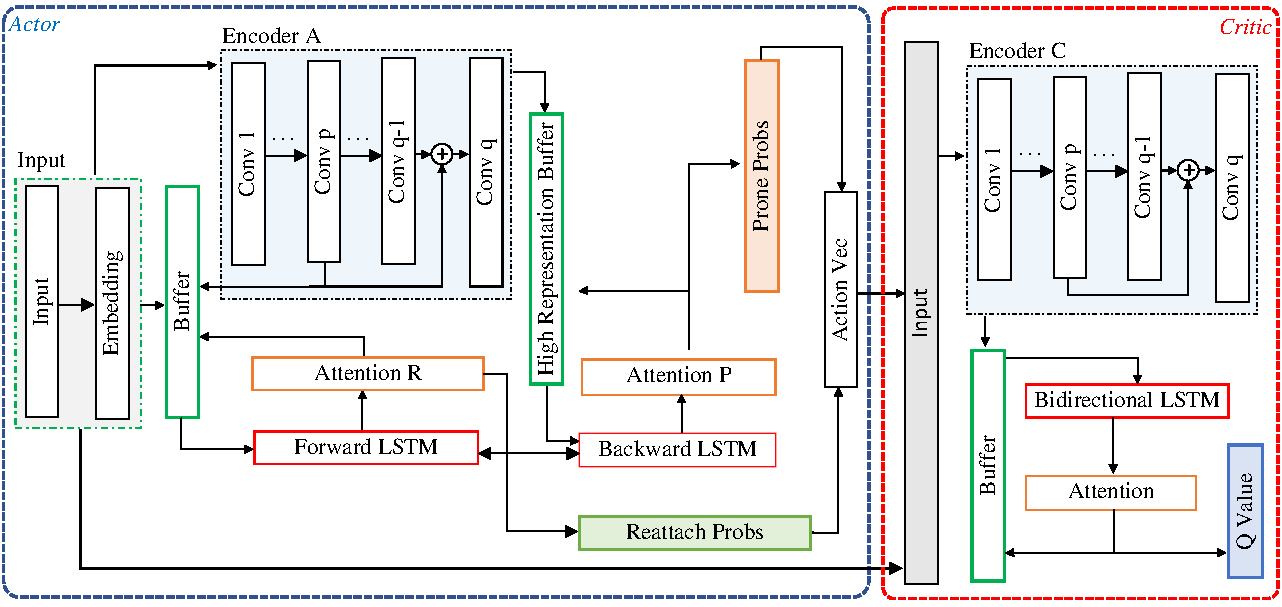
\includegraphics[width=1.002\textwidth]{img/chaps/pm/network}
	\caption{ساختار معماری شبکه پیشنهادی}    
	\label{fig:ch_pm:main_network}
\end{figure}
در ابتدا یک بخش \lr{input} خواهیم داشت که ورودی‌ها را دریافت و آن‌ها را به فرمی قابل بررسی از \gls{featurevector} تبدیل خواهد کرد.
اگر ماتریس $D$ ما به تعداد $N$ نمونه (سطر) و $M$ جهش (ستون) داشته باشد در آن صورت ماتریس $I'$ ما دارای ابعاد $(M\times N, 4)$ خواهد بود که در کل فضای حالت $4MN$ را خواهند داشت که $MN$ بخاطر دو ستون اول ماتریس $I'$ است که هر سطر با دیگری متفاوت است و $4$ بخاطر دو ستون انتهایی ماتریس $I'$ است که هرکدام $4$ حالت مختلف را می‌توانند داشته باشند که در مجموع فضای حالت $4MN$ را می‌توانند اختیار کنند. هر داده از این ماتریس ورودی را به برداری به طول $2$ \lr{embed} می‌کنیم که خروجی برداری به ابعاد $(M\times N, 4, 2)$ خواهد شد که حال این  \glspl{floatnumber} که در یک رنج و ارزش هستند، بعد از یک تغییر بعد به صورت $(M, N, 8)$ نمایش می‌دهیم. حال این داده‌ها آماده استخراج ویژگی و اعمال عملیات کانولوشنی بر رویشان هستند. 
\\
پس از آن وارد بخش \gls{encoder} می‌شویم. در این بخش دو خروجی با سایز ماتریس ورودی $I'$ خواهیم داشت که یکی از آن‌ها ویژگی‌های با فرکانس بالاتر در آن قرار دارد و دیگری به علت عمیق‌تر بودن عملیات استخراج ویژگی شامل اطاعاتی با توصیف‌های سطح بالاتر از داده‌ها می‌باشد. سپس از این دو خروجی به صورت خوانش‌های در جهت عکس یکدیگر استفاده خواهد شد. در این خوانش‌ها با کمک گرفتن از ماژول‌های \lr{LSTM} به عنوان حافظه‌هایی که مدل‌سازی تبدیل فضای ماتریس به حالت درخت را بر عهده خواهند داشت اطلاعات در در هر محله با یکدیگر به اشتراک می‌گزارند و در ادامه یک \gls{attentionlayer} که با افزایش خوانش‌ها از یک حالت تصادفی آموزش می‌یابد که در آن فضا ابعاد متفاوت داده‌ها چگونه ارزش‌گزاری شوند که جهش‌‌های مناسب در نهایت مورد توجه باشد قرار گرفته است. در نهایت هر کدام از این هدرها برای یک منظور به کمک اطلاعات استخراجی درون \lr{LSTM}ها خروجی‌های احتمالاتی‌ای تولید خواهند کرد که یکی برای انتخاب محل برش و دیگری مکانی برای گسترش و اتصال مناسب مورد استفاده قرار خواهند گرفت.
\\
این مجموعه به طور کلی ماژول \gls{actor} ما را شامل می‌شود که خروجی‌های تصمیم‌گیری برای ما تولید می‌کند. در ادامه در ماژول \gls{critic} این خروجی‌های تولید شده به همراه شرایط فعلی به عنوان ورودی با یکدیگر ادغام می‌شوند تا از اطلاعاتی که از آن‌ها استخراج می‌شود شبکه بتواند این تصمیم‌گیری را در جهت رسیدن به پاسخ مطلوب ارزش‌گزاری کند که این بخش نیز مشابه با بخش ابتدایی شامل یک \gls{encoder} است که از خروجی حاصل با استفاده از دو خوانش به صورت \gls{bidirectional} مقدار \lr{Q-Value} تخمین زده می‌شود.


\section{جمع‌بندی و نتیجه‌گیری}
در این فصل روش پیشنهادی خود را به تفضیل شرح دادیم که الگو گرفته شده از روش ارائه شده در مقاله \lr{scite} بود اما با این تفاوت که در آنجا فرض مکان‌های بی‌نهایت بود ولی ما فرضی که در روش \lr{scarlet} معرفی شده بود را جایگزین کردیم که اجازه می‌داد با توجه به شواهدی که از داده‌های مکمل \gls{cnv} استخراج شده است، بعضی از \glspl{gene} پس از وقوع حذف شوند که در این بین چون فضای جست و جو بزرگ‌تر شد در نتیجه مجبور شدیم نحوه برداشتن گام‌های خود را تغییر دهیم و هوشمندانه‌تر پیش رویم که در این فضای بزرگ‌تر بتوانیم به جواب مناسب برسیم. در \lr{scite} برای رسیدن به درخت بهتر به دنبال تنظیم کردن پارامترهای خطا بود در حالی که ممکن بود با جواب واقعی فاصله داشته باشد اما چون بدنبال جواب با امتیاز بالا بود در نتیجه این پارامتری بودن و جست و جو برای مقادیر بهینه خطا در روش آن وجود داشت اما ما برای بهتر کردن امتیاز به جای تغییر پارامترهای خطا به ازای یک درخت، جست و جوی ضمیمه کردن‌های مختلف سلول‌ها و امکان فقدانشان را پس از وقوع در درخت جست و جو می‌کنیم.








%\section{روش پیشنهادی دوم}
%
%\subsection{مقدمه}
%
%\subsection{دادگان ورودی}
%
%\subsection{تبدیل داده‌ها به بردار ویژگی}
%
%\subsection{مدل‌سازی مساله}
%
%\subsubsection{معماری شبکه}
%
%\subsection{تابع هزینه}
%
%\subsection{اصلاح خطا و یافتن درخت جواب}

%\begin{table}[ht]
%	\caption{پارامترهای مدل ریاضی}
%	\label{tab:modelParameters}
%	\centering
%	\onehalfspacing
%	\begin{tabularx}{0.9\textwidth}{|r|X|}
%		\hline
%		$t_{ik}$			& زمان خدمت‌دهی به بیمار در مرحله $k$ام \\
%		\hline
%		$\tilde{t}_{ik}$	& زمان فاری خدمت‌دهی به بیمار در محله $k$ام \\
%		\hline
%		$t_{ik}^p$			& مقدار بدبینانه (حداکثر) برای زمان خدمت‌دهی به بیمار در مرحله $k$ام \\
%		\hline
%		$t_{ik}^m$			& محتمل‌ترین مقدار برای زمان خدمت‌دهی به بیمار در مرحله $k$ام \\
%		\hline
%		$t_{ik}^o$			& مقدار خوشبینانه (حداقل) برای زمان خدمت‌دهی به بیمار در مرحله $k$ام \\
%		\hline
%	\end{tabularx}
%\end{table}
%
%\begin{table}[ht]
%	\caption{متغیرهای مدل ریاضی}
%	\label{tab:modelVariables}
%	\centering
%	\onehalfspacing
%	\begin{tabularx}{0.9\textwidth}{|r|X|}
%		\hline
%		$X_{ild_{k}}$	& متغیر صفر-یک تخصیص بیمار به تخت/اتاق عمل\\
%		\hline
%		$S_{ild_{k}}$	& زمان شروع خدمت‌دهی به بیمار \\
%		\hline
%		$Y_{ijkl_{k}}$	& متغیر صفر-یک توالی بیماران \\
%		\hline
%		$V_{ni}$		& متغیر صفر-یک تخصیص جراح به بیمار‍‍ \\
%		\hline
%	\end{tabularx}
%\end{table}
		% فصل چهارم: روش پیشنهادی
% !TeX root=../../../main.tex

\chapter{نتایج تجربی}

تا به اینجا مسئله پیش رو و ابعاد پیچیدگی آن مشخص شده است. همچنین حوزه‌های درگیر و مفاهیم مرتبط را نیز بازگو شده است و پس از آن مفروضات و روش‌های مختلف مرتبط برای حل مسئله بررسی شد. 
در نهایت در فصل گذشته نیز رویکرد پیشنهادی در این پایان‌نامه برای پاسخ به این مسئله ارائه گشت. حال در این فصل قصد داریم تا در عمل روش پیشنهادی خود را بسنجیم و نتایج حاصل از آن را مشاهده نماییم.
\\
به همین منظور در این فصل ابتدا پایگاه داده‌ای مجازی تهیه می‌کنیم و در ادامه نحوه استفاده از روش پیشنهادی و آموزش و استفاده از شبکه طراحی شده را خواهیم گفت. پس از آن به نتایج بدست آمده بر روی پایگاه داده مصنوعی می‌پردازیم و حالات مختلف آن را مورد ارزیابی قرار می‌دهیم و در نهایت نتیجه اجرای روش پیشنهادی خود را بر روی یک داده حقیقی مشاهده خواهیم نمود.

\section{پایگاه داده‌های ورودی}
قبل از اینکه وارد روش پیشنهادی شویم به تشریح وردی‌های مسئله و داده‌هایی که مورد استفاده قرار خواهیم داد می‌پردازیم.
داده‌های ورودی برابر ماتریس $D_{m\times n}$ می‌باشد که بعد اول $M$ برابر با ژن‌ها و بعد دوم $N$ برابر سلول‌های نمونه‌برداری شده می‌باشد. در هر خانه $d_{i,j}$ یک بردار داده قرار دارد که حاوی اطلاعات ژن $j$ در سلول $i$ می‌باشد.

\subsection[پایگاه داده مصنوعی]
{پایگاه داده مصنوعی
	\LTRfootnote{Synthetic Dataset}
}

با توجه به این نکته که از درخت فیلوژنی حقیقی\LTRfootnote{Ground-truth Phylogeny Tree} داده‌های حقیقی موجود اطلاعی نداریم، به سراغ ساخت پایگاه‌ داده مصنوعی می‌رویم. با استفاده از این پایگاه داده مصنوعی می‌توانیم در مورد روش‌هایی که در ادامه بیان خواهیم کرد یک معیار ارزیابی نسبتا مناسبی داشته باشیم و تا حدودی از مشکلات روش‌های پیشنهادی آگاه شویم و به تصحیح آن بپردازیم. برای ساخت پایگاه داده مصنوعی که همان ماتریس ورودی $D_{m\times n}$ می‌باشد، از دو روش مختلف با دو فرض مختلف استفاده خواهیم کرد که در ادامه به تشریح هر کدام خواهیم پرداخت.


در ادامه جدول
\ref{tab:ch_er:datasetIndices}
را برای معرفی اندیس‌های بکار گرفته شده در روابط مربوط به تولید پایگاه‌داده مجازی بیان می‌نماییم.
\begin{table}[ht]
	\caption{اندیس‌های به کار رفته در تولید پایگاه داده مجازی}
	\label{tab:ch_er:datasetIndices}
	\centering
	\onehalfspacing
	\begin{tabularx}{0.9\textwidth}{|r|X|}
		\hline
		$D$	& ماتریس داده نویزی در دسترس که مقادیر $0$، $1$ و $3$ (به عنوان داده از رفته) در آن قرار دارد \\
		\hline
		$E$	& ماتریس داده حقیقی بدون نویز که به دنبال آن هستیم \\
		\hline
		$T$	& درخت فیلوژنی جهش‌ها \\
		\hline
		$C$ & پروفایل تعداد کپی نمونه‌ها \\
		\hline
		$N$	& تعداد سلول‌های نمونه \\
		\hline
		$M$	& تعداد جهش‌ها \\
		\hline
		$\alpha$ & نرخ خطای \gls{falsepositive} \\
		\hline
		$\beta$	& نرخ خطای \gls{falsenegative} \\
		\hline
		$\zeta$ & پارامتر تعیین‌کننده میزان چاقی و لاغری درخت‌ \\
		\hline
		$\gamma$ & پارامتر تعیین‌کننده میزان ادغام جهش‌ها در یک گره (عدم مشاهده نمونه بینشان) \\
		\hline
		$\psi$ & تعیین‌کننده احتمال فقدان یک جهش \\
		\hline
		$\vartheta$ & تعیین‌کننده میزان تاثیر در وقوع فقدان متناسب با فاصله از وقوع جهش \\
		\hline
		$\varrho$	& احتمال کاهش تعداد کپی بدون از دست رفتن جهش \\
		\hline
	\end{tabularx}
\end{table}
\\
برای ایجاد پایگاه داده در این حالت ابتدا درختی تصادفی با پارامترهای $\zeta, n$ ایجاد می‌کنیم که $n$ تعداد ژن‌ها (جهش‌ها) بوده و $\zeta$ عددی در بازه $(0, \infty)$ است که یک پارامتر کنترلی است که وظیفه‌اش کنترل کلی تعداد نسل‌های مختلف را از یک جمعیت در درخت فیلوژنی می‌باشد.
حال برای تولید پایگاه داده مصنوعی به ترتیب چهار گام زیر باید انجام شود.
\begin{itemize}
	\item ایجاد یک درخت فیلوژنی تصادفی
	\item مشخص کردن برخی ژن‌ها برای حذف در ادامه و تولید پروفایل تعداد کپی
	\item تبدیل درخت فیلوژنی حاصل به ماتریس اطلاعات سلول-ژن ($E$)
	\item اضافه کردن نویز به ماتریس $E$ و تبدیل آن به ماتریس نویزی $D$
\end{itemize}
در ادامه هر بخش به صورت جداگانه به تفضیل شرح داده خواهد شد.

\subsubsection{ساخت درخت تصادفی}
برای ساخت درخت تصادفی از دو روش مختلف استفاده شده است که هرکدام جداگانه توضیح داده شده است.
\vspace{20pt}
\\
\textbf{روش اول: با استفاده از\gls{randombinarygenealogicaltree}}
\\
در این روش همان‌گونه که از نام آن مشخص است با استفاده از درخت تصادفی دودویی ژنولوژی به ساخت ماتریس داده ورودی مسئله می‌پردازیم که برای ساخت این دادگان از فرض‌های که در ادامه آمده است استفاده خواهیم کرد. 

در مرحله اول که ساخت درخت است به این صورت عمل میکنیم که به تعداد $n$ گونه (سلول) در نظر می‌گیریم. سپس به ترتیب مراحل زیر را انجام می‌دهیم تا به درخت تصادفی مورد نظر برسیم.
\begin{itemize}
	\item به هر کدام از $n$ گونه متمایز در ابتدا وزن $w_i=1$ را اختصاص می‌دهیم که متناسب با احتمال انتخاب هر گونه در مراحل بعدی خواهد بود.
	\item برای هر گونه ‌$i$ تابع جرم احتمال را در ادامه به صورت $F_i=\frac{w_i}{\sum_{i=1}^{n}w_i}$ در نظر میگیریم
	\item با استفاده از $F$ دو گونه متمایز $u, v$ را انتخاب می‌کنیم و به هم متصل می‌کنیم
	\item به جای دو گونه $u, v$ یک گونه جدید $uv$ با وزن $w_{uv}=\frac{w_u+w_v}{\sqrt[4]{\zeta}}$ را قرار می‌دهیم.
	\item تعداد گونه‌ها یک واحد کم شده است. بررسی می‌کنیم اگر تعداد گونه‌های باقی‌مانده از $2$ کمتر باشد درخت تصادفی ساخته شده است و پایان کار است. در غیر این صورت به مرحله اول بازمی‌گردیم.
\end{itemize}
پارامتر $\zeta$ به گونه‌ای کنترل‌کننده میزان ناپایداری در طی نسل‌ها می‌باشد. بطوریکه نمونه‌ای از نتایج مقادیر مختلف آن برای $n=20$ در شکل \ref{fig:dsismn20} آورده شده است. پس از ساخت درخت تصادفی به سراغ مرحله بعد یعنی تبدیل درخت به ماتریس ژن-سلول $E$ می‌رویم.
\begin{figure}[!ht]
	\centering
	\subfloat[$\zeta=0.2$]{
			\centering
			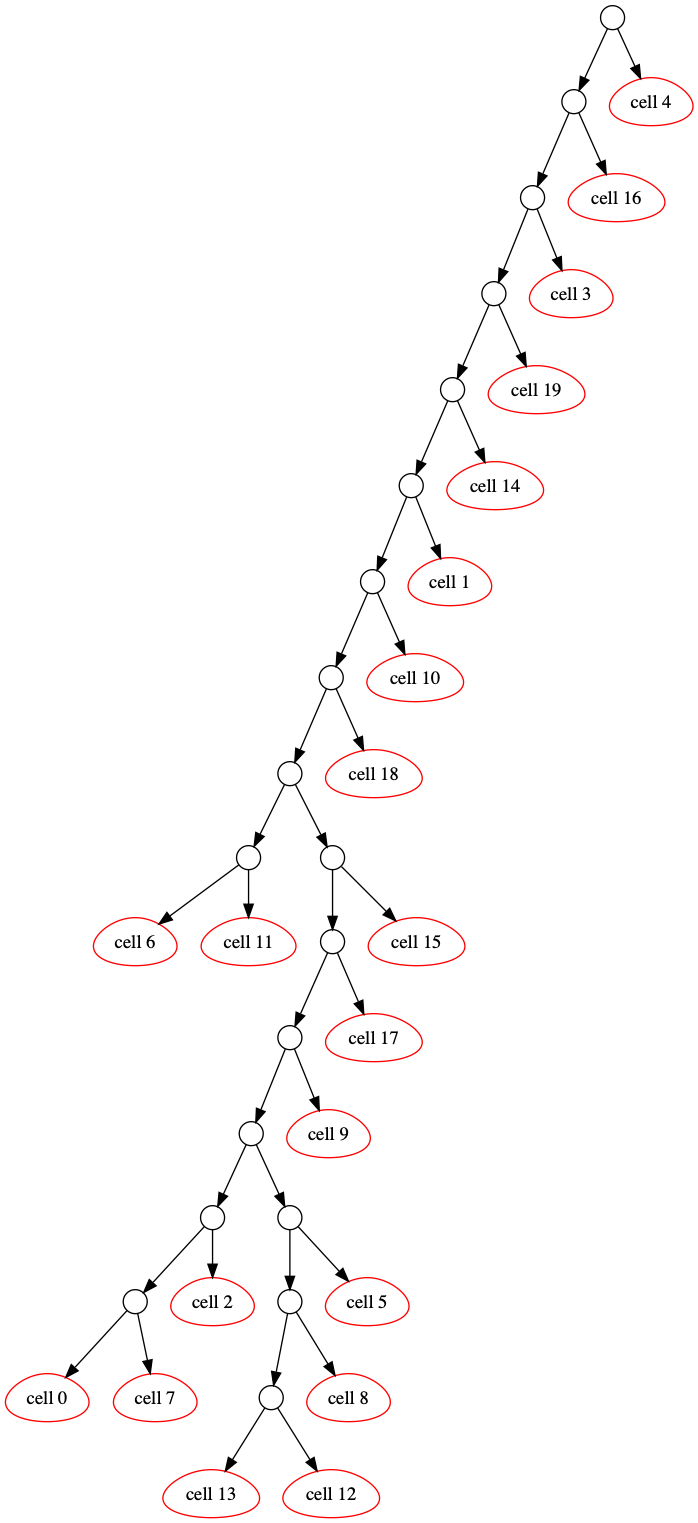
\includegraphics[width=0.48\textwidth, height=0.42\textheight]{img/dataset/s/n20_zeta02}
			\label{fig:dstn20zeta0.2}
	}
	\hfill
	\subfloat[$\zeta=1.0$]{
			\centering
			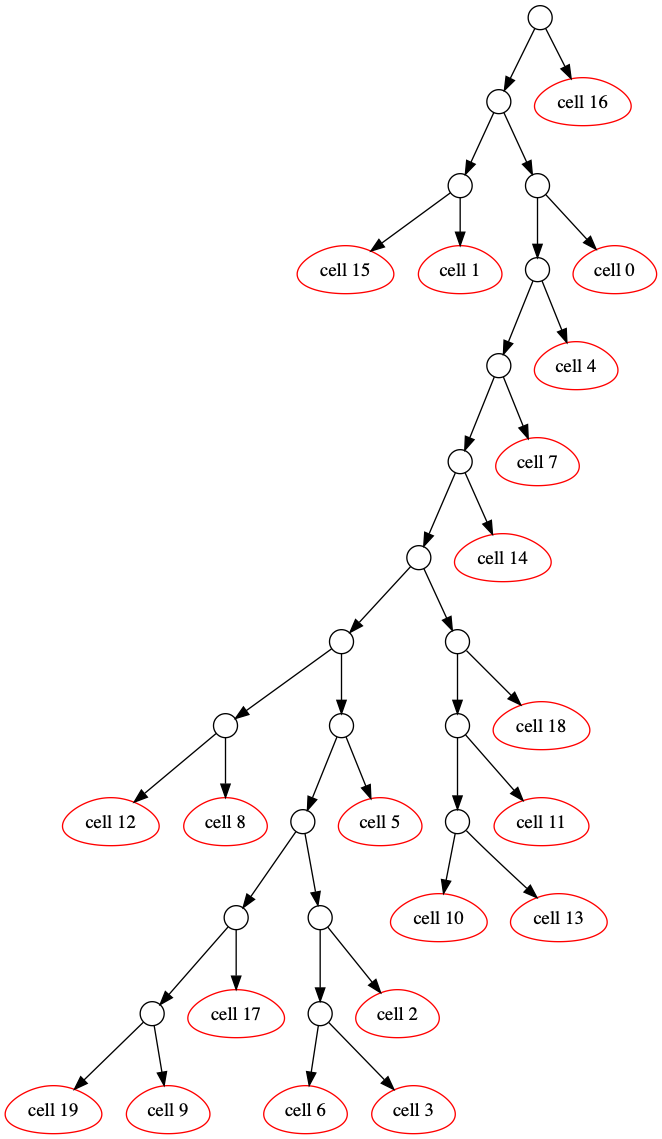
\includegraphics[width=0.48\textwidth, height=0.42\textheight]{img/dataset/s/n20_zeta1}
			\label{fig:dstn20zeta1}
	}
	\hfill
	\vskip\baselineskip
    \subfloat[$\zeta=8$]{
    	\centering
    	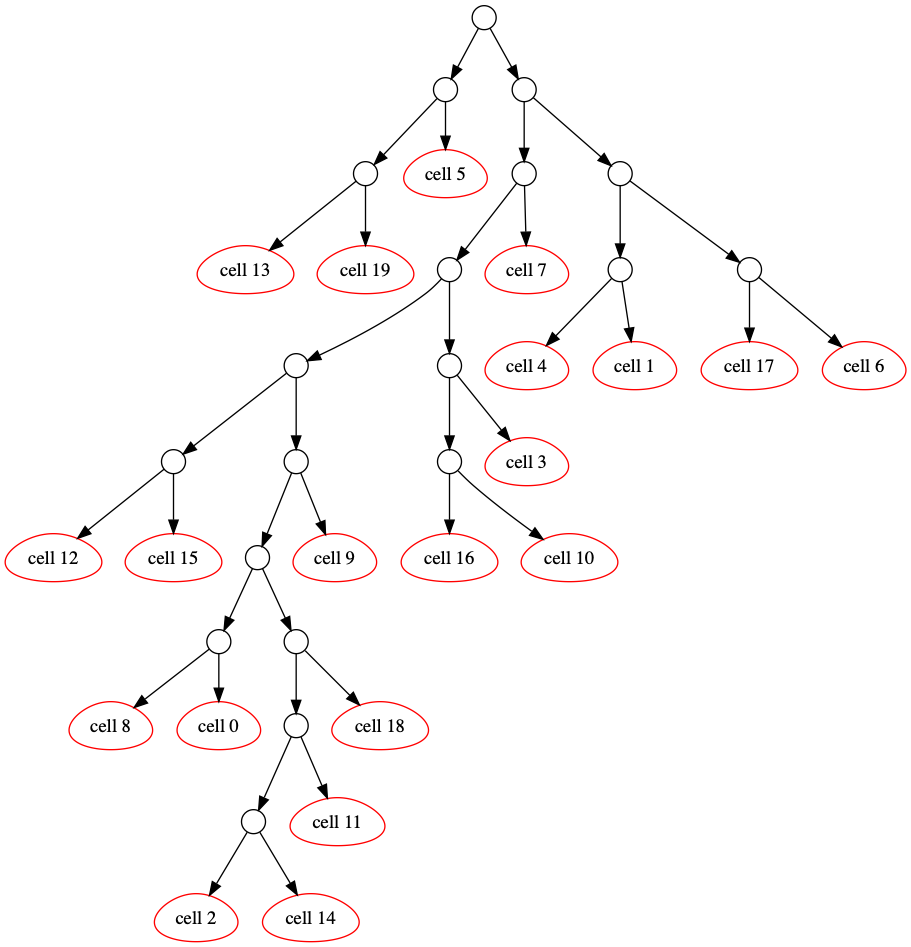
\includegraphics[width=0.38\textwidth, height=0.27\textheight]{img/dataset/s/n20_zeta8}
    	\label{fig:dstn20zeta8}
    }
	\hfill
	\subfloat[$\zeta=100$]{
		\centering
		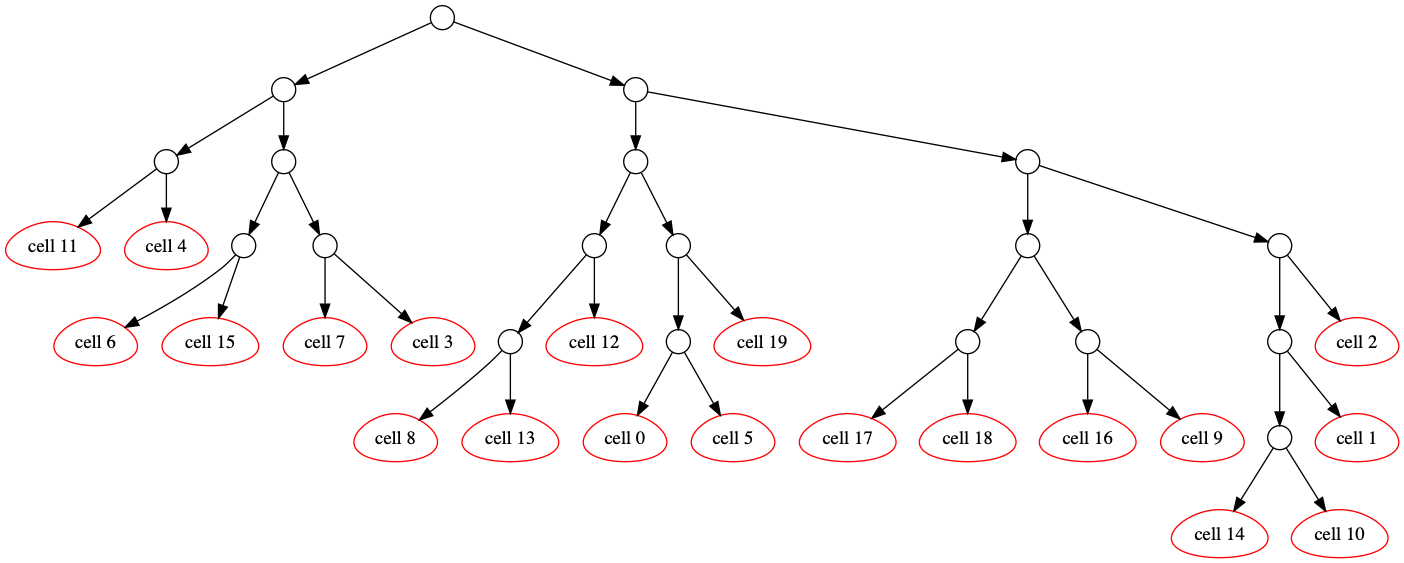
\includegraphics[width=0.58\textwidth, height=0.22\textheight]{img/dataset/s/n20_zeta100}
		\label{fig:dstn20zeta100}
	}
	\caption{درخت فیلوژنی تصادفی تولید شده برای $n=20$ و $\zeta$های مختلف}
	\label{fig:dsismn20}
\end{figure}
\\
در ادامه با توجه به اینکه تعداد دلخواه جهش‌ها چه عددی بوده است یکی از گام‌های زیر را برمی‌داریم.

\begin{itemize}
	\item اگر تعداد جهش‌ها $M>N$ بوده باشد در آن صورت به صورت تصادفی به تعداد دفعات اختلاف یکی از انشعاب‌ها در درخت را به صورت تصادفی انتخاب کرده و آن جهش اضافه شده را تا تمامی نوادگان پیش خواهیم برد.
	\item اگر تعداد جهش‌ها $M<N$ بوده باشد آنگاه مجددا به اندازه تعداد اختلاف انشعاب‌هایی را انتخاب کرده و این بار جهش در آن انشعاب را تا تمامی نوادگان حذف می‌کنیم.  
\end{itemize}
به این ترتیب تمامی سلول‌ها را با تعداد جهش‌های انتخابی خواهیم داشت. در نهایت برای اخرین تغییر در جهش‌ها می‌توان یک گام دیگر برداشت که آن تولید یه عدد تصادفی کوچکتر از $\frac{M}{2}$ است که به آن تعداد می‌توان جهش‌های موجود را از انشعابی برداشت و بر روی انشعابی دیگر قرار داد. با این کار ممکن است تعداد جهش‌ها در انشعاب‌های مختلف تغییر کند و چه بسا به مدل‌های واقعی نزدیکتر شود که البته در این پایان‌نامه از گام آخر صرف‌نظر کرده‌ایم.
\\
حال کار ما با پخش تصادفی جهش‌ها در پایگاه‌داده مجازی پایان یافته است. تا به اینجا ما در فرض خود از هر نمونه جمعیت مختلف یک سلول داشته‌ایم. اما  در بعضی مواقع در پایگاه داده‌های واقعی ممکن است از یک جمعیت بیش از یک نمونه وجود داشته باشد که البته این امر لزوما درست نیست به این دلیل که بعد از افزوده شدن نویز به داده‌ها ممکن است برخی سلول‌ها جهش‌هایشان مشابه هم شود. اما به هرحال اگر چنین چیزی را بخواهیم که داشته باشیم با انتخاب تصادفی برخی سلول‌ها(برگ‌ها) در درخت و کپی کردن آن‌ها می‌توان به چنین مقصودی رسید.
\vspace{20pt}
\\ \textbf{روش دوم: با استفاده از درخت تصادفی جهش‌های ژنی}	\LTRfootnote{Random Mutation History Tree}
\\
این روش نیز تا حدود زیادی مشابه روش قبل است با این تفاوت که در اینجا به جای اینکه درخت تصادفی را با توجه سلول‌ها از پایین به بالا بسازیم، ابتدا یک درخت تصادفی بدون در نظر گرفتن سلول‌ها ایجاد می‌کنیم و سپس به تخصیص جهش‌ها به آن می‌پردازیم. در نهایت برای آخرین مرحله به تعداد دلخواد سلول را به درخت اضافه کرده و درخت را تکمیل می‌کنیم. در گام اول به تعداد $M+1$ نود در نظر می‌گیریم. مشابه حالت قبل با طی مراحلی که در ادامه آمده است به ساختار یک درخت تصادفی می‌رسیم.
\begin{itemize}
	\item به هر کدام از $m$ نود متمایز در ابتدا وزن $w_i=1$ را اختصاص می‌دهیم که متناسب با روند حرکتی تومور به سمت آن جهش‌ها در مراحل بعدی خواهد بود.
	\item برای هر نود ‌$i$ تابع جرم احتمال را در ادامه به صورت $F_i=\frac{w_i}{\sum_{i=1}^{n}w_i}$ بیان می‌شود در نظر می‌گیریم.
	\item با استفاده از $F$ دو نود متمایز $u, v$ را انتخاب می‌کنیم و به هم متصل می‌کنیم
	\item به جای دو گونه $u, v$ یک نود جدید $uv$ با وزن $w_{uv}=\frac{w_u+w_v}{\sqrt[4]{\zeta}}$ را قرار می‌دهیم.
	\item تعداد نود‌ها یک واحد کم شده است. بررسی می‌کنیم اگر تعداد نود‌های باقی‌مانده از $2$ کمتر باشد به مرحله بعد می‌رویم و در غیر این صورت به مرحله اول بازمی‌گردیم.
	\item در این مرحله تمامی برگ‌های درخت ساخته شده را حذف می‌کنیم و تنه باقی‌مانده را به عنوان درخت تصادفی جهش‌ها در نظر می‌گیریم.
\end{itemize}

پس از به پایان رسیدن مراحلی که بیان شد درخت تصادفی آماده است و حال نوبت به تخصیص دادن خود ژن‌ها به هرکدام از این نودهای درخت است. برای این منظور به هرکدام از $M$ نود یک ژن را به صورت تصادفی تخصیص می‌دهیم. پس از آن برای نهایی سازی درخت جهش‌ها از پارامتر دلخواه 	$A = \lfloor\gamma*(M-1)\rfloor$ استفاده می‌کنیم که $\gamma$ عددی بین $(0,1)$ است و $A$ تعداد یال‌هایی است که در درخت باید برداشته شود و دو نود آن با یکدیگر ادغام شود. این کار باعث می‌شود تا در درخت جهش‌ها در برخی نودها به جای یک جهش چند جهش داشته باشیم که بتواند به مدل داده‌های واقعی نزدیکتر باشد.
\\
پس از تکمیل درخت جهش‌ها نوبت قرار دادن نمونه‌هایی بر روی آن است. به همین منظور با فرض اینکه $N\ge M$ است. به تعداد $M$ تا از سلول‌ها را به هر کدام از نودهای درخت جهش به عنوان برگ‌های جدید اضافه می‌کنیم و برای $N-m$ سلول باقی مانده همین کار را این‌بار به صورت تصادفی انجام می‌دهیم. در نهایت درخت تصادفی جهش‌ها ساخته شده است که نمونه‌ای از آن را در شکل \ref{fig:mtn30m20z1g0.15} قابل مشاهده است.
\begin{figure}
	\centering
	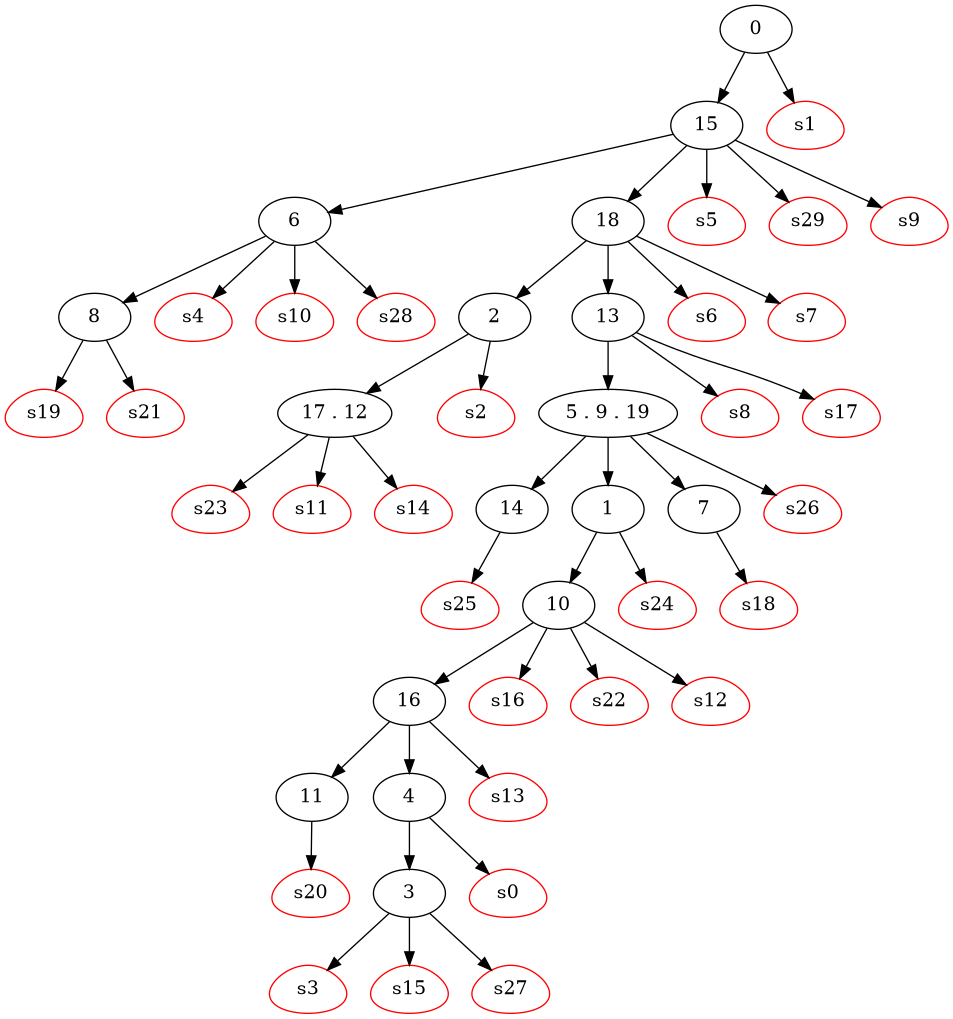
\includegraphics[width=0.62\textwidth]{img/dataset/s/treeF_zeta=1_gamma=0.15_alpha=0.01_beta=0.1_MR=0.02_N=30_M=20.png}
	\caption{درخت جهش تصادفی با پارامتر‌های $N=30, M=20, \zeta=1, \gamma=0.15$}
	\label{fig:mtn30m20z1g0.15}
\end{figure}

\subsubsection{تبدیل درخت به ماتریس ژن-سلول}
با داشتن درخت (تولید شده با هرکدام از روش‌ها تفاوتی ندارد) در ادامه ابتدا از روش مدل‌سازی \glspl{infinitesites} ماتریس را تشکیل می‌دهیم و پس از آن فرض حذف برخی از جهش‌ها را در آن مشابه با مقاله \lr{scarlet} اضافه می‌کنیم و پروفایل‌های تغییر تعداد کپی را به عنوان داده‌های تکمیلی برای درخت و داده‌های \gls{snv} می‌سازیم.
%\vspace{20pt}
\\
\noindent\textbf{فرض مدل مکان‌های بی‌نهایت}\LTRfootnote{Infinite Sites Model}\\
در این حالت فرض می‌کنیم که هر جهش اتفاق افتاده در درخت فیلوژنی در تمامی نسل‌های پس از آن باقی می‌ماند و هیچ‌گاه از بین نمی‌رود. در چنین حالتی درخت حاصل از این روش درختی یکتا بوده که به نام درخت فیلوژنی کامل\LTRfootnote{Perfect Phylogeny Tree} شناخته می‌شود.
\\
در این قسمت باید با استفاده از درخت تصادفی تولید بتوانیم ماتریس جهش‌ها را برای سلول‌های مختلف با فرض مکان‌های بی‌نهایت بدست آوریم. 
در ابتدا ماتریس $E$ را به ابعاد $M\times N$ ایجاد می‌کنیم و برای هر درایه $i,j$ در آن که $i$ شماره جهش و $j$ شماره سلول است به صورت فرمولی که در ادامه آمده است مقداردهی می‌کنیم.
\begin{equation}
	E_{i,j} = 
	\begin{cases} 
		1  \quad &\text{\lr{if}} \quad \text{\lr{mutation }} i \text{\lr{ is an ancestor of cell }} j \\
		0 \quad &\text{\lr{o.w}}
	\end{cases}
\end{equation}
به این ترتیب با فرض مدل مکان‌های بی‌نهایت ماتریس بدون خطا $E$ را داریم که در گام بعد آن‌ها ممکن است این فرض برایشان نقض شود و جهش‌هایی پس از وقوع حذف شوند.

\subsubsection{تولید پروفایل‌های تعداد کپی و تعیین جهش‌های مسافر}
پس از ساخت درخت و تبدیل آن به ماتریس $E$ طبق فرض مدل مکان‌های بی‌نهایت، حال با توجه به مقدار پارامترهای $\psi$، $\vartheta$ و $\varrho$ به تغییر در ساختار ماتریس $E$ و ساخت داده‌های پروفایل تعداد کپی می‌پردازیم.
پارامتر $\psi$ تعیین ‌کننده احتمال فقدان یک جهش، پارامتر $\vartheta$ میزان تاثیر در وقوع فقدان متناسب با فاصله از وقوع جهش و پارامتر $\varrho$ احتمال کاهش تعداد کپی بدون از دست رفتن جهش را کنترل می‌کنند.
\\
حال که درخت را داریم کافی است تا برگ‌ها را کنار بگذاریم و از بین نود‌های باقی مانده در درخت $T$، با احتمال مشخص شده $\psi$ جهش‌ها را برای حذف انتخاب ‌کنیم. دلیل کنار گذاشته شدن برگ‌ها نیز مشخص است زیرا که اگر آن‌ها قرار باشد حذف شوند چون برگ هستند دیگر زیر درختی ندارند که بخواهند حذف خود را در آن‌جا رقم بزنند. پس در نتیجه دقت شود که از روی این پارامتر تعداد جهش‌های حذف‌شونده را نمی‌توان حدس زد و تعداد آن‌ها به چاقی یا لاغری درخت بستگی دارد بطوریکه هرچه درخت لاغرتر باشد در آن صورت این احتمال به تعداد حذف شده‌ها نزدیکتر خواهد بود و بلاعکس.\\
پس از مشخص شدن جهش‌های حذف‌شونده حال زیردرخت‌های آن‌ها را جدا می‌کنیم و متناسب با پارامتر $\vartheta$ یکی از نودهای نوادگان را به عنوان محل فقدان انتخاب می‌کنیم. این عمل طبق رابطه \ref{eq:ch_er:loss_loc} انجام می‌شود.
\begin{equation}
	P_l(x|i) = \vartheta e^{-\vartheta *\text{\lr{dist($x$,$i$)}}}
	\label{eq:ch_er:loss_loc}
\end{equation}
این رابطه همان توزیع نمایی است که برای فضای پیوسته تعریف شده است. ما فاصله نودهای زیردرخت ($x$) را به جهش انتخاب شده $i$ در زیر درخت آن ژن در نظر می‌گیریم و متناسب با این رابطه و احتمال یکی از آن‌ها را به عنوان محل فقدان انتخاب می‌کنیم. مشخص است که هر چه این مقدار پارامتر کوچکتر باشد این انتخاب محل فقدان به فاصله تا ژن انتخابی کمتر تاثیرگذار می‌شود.
\\
در نهایت پس از این مرحله نوبت به تولید پروفایل‌های تعداد تکرار برای نمونه‌ها می‌رسد. ما بردار پروفایل تکرار را $k$ واحد درنظر می‌گیریم و ژن‌ها را در بین آن‌ها توزیع می‌کنیم. در این پایگاه داده تمرکز ما در تولید این پروفایل‌ها به مقادیر کپی‌ها نیست بلکه به نحوه تغییر آنهاست که افزایشی است یا کاهشی. بنابرین با یک مقدار اولیه تصادفی نمونه‌های اولیه که به ریشه متصل شده‌اند را مقداردهی می‌کنیم و در ادامه با توجه به اینکه محل اتصال نمونه‌ها کجاست آن‌ها را بدون تغییر باقی میگذاریم یا فقط افزایش می‌دهیم. پس از این کار ژن‌های انتخاب شده برای حذف را به همراه درصدی که پارامتر $\varrho$ مشخص می‌کند را درون یک لیست می‌گذاریم و تمام نمونه‌های مرتبط با آن‌ها را به صورت تصادفی بین $1$ تا $3$ واحد کاهش می‌دهیم تا پروفایل‌های $C$ برای نمونه‌ها ساخته شود.\\
مشخص است که این عملیات هیچ تغییری در ساختار درخت ایجاد نمی‌کند و صرفا کافی است در کنار داده‌های ساخته شده ‌$C$، در درخت، نودهای حذف شونده و محل حذف آن‌ها را مشخص کنیم تا آماده ورود به مرحله بعد که ساخت ماتریس از روی این درخت است برویم.
\\
در نهایت خروجی این بخش برای تصاویر درختان تولید شده قبل در شکل \ref{fig:E} قابل مشاهده می‌باشند. 
\begin{figure}[!ht]
	\centering
	\subfloat[ماتریس درخت شکل \ref{fig:dstn20zeta1}]{
		\centering
		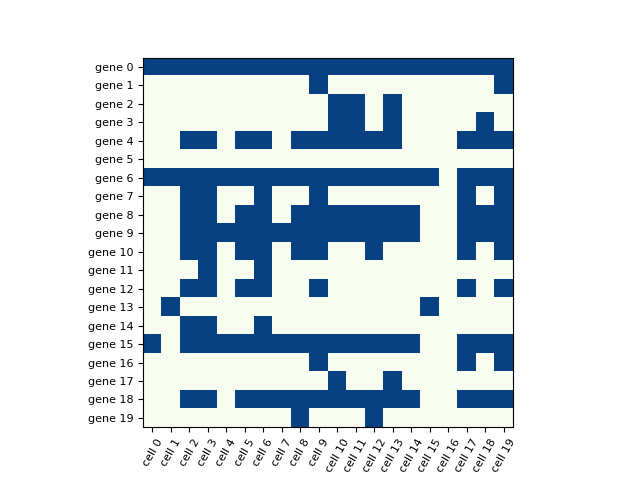
\includegraphics[width=0.55\textwidth]{img/dataset/s/zeta1n20m20}
		\label{fig:Edstn20zeta1}
	}
	\hfill
	\subfloat[ماتریس درخت شکل \ref{fig:mtn30m20z1g0.15}]{
		\centering 
		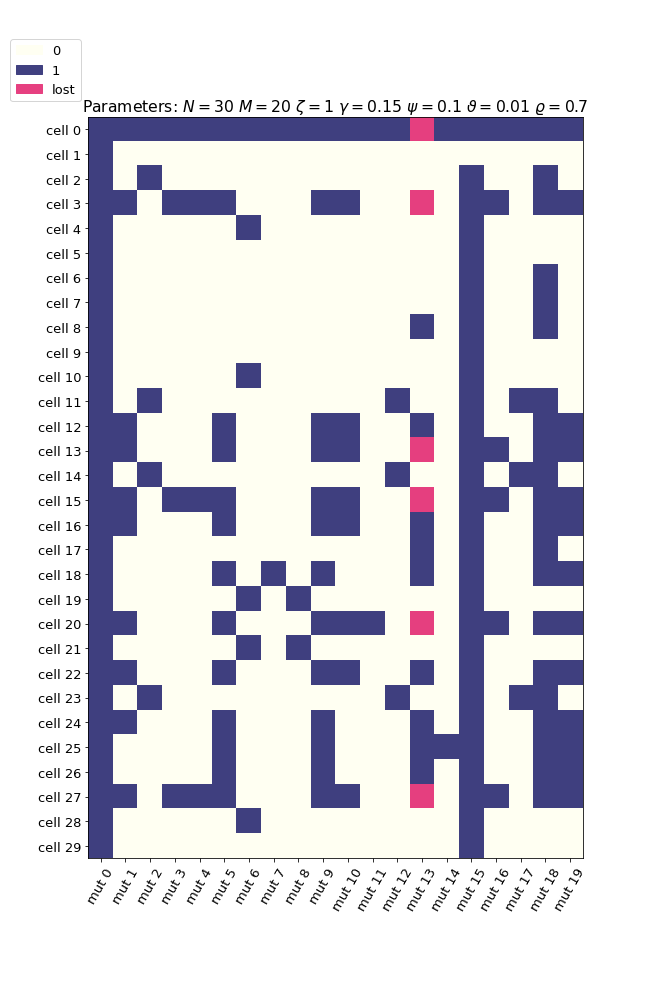
\includegraphics[width=0.42\textwidth]{img/dataset/s/El_zeta=1_gamma=0.15_alpha=0.01_beta=0.1_MR=0.02_N=30_M=20.png}
		\label{fig:E_mt_N30_M20_Z1_G0.15}
	}
	\caption{ماتریس‌های ژن-سلول ($E$) بدست آمده از درخت‌های تصادفی ساخته شده}
	\label{fig:E}
\end{figure}
همانطور که مشخص است برای یکی از درختان فقدان یک جهش بوجود آمده است و برای دیگری نه. 
\subsubsection{اضافه کردن نویز به ماتریس ژن-جهش}
برای قسمت نهایی آماده‌سازی پایگاه داده مجازی نیاز است تا به ماتریس $E$ با پارامتر $\Theta=(\alpha, \beta, m_r)$ نویز اضافه کنیم و آن را به ماتریس $D$ تبدیل کنیم که $\alpha=P(D_{ij}=1|E_{ij}=0)$ و $\beta=P(D_{ij}|E_{ij})$ است و همچنین $m_r\in(0,1)$ که نرخ داده‌های از دست رفته را مشخص می‌کند.
\\
برای این منظور به ازای تمامی درایه‌های $0$ ماتریس $E$ هربار یک عدد تصادفی با توزیع یکنواخت بین $[0,1)$ بوجود می‌آوریم و اگر عدد تولید شده کوچکتر از $\alpha$ بود آنگاه ان درایه در ماتریس $D$ را برابر با $1$ قرار می‌دهیم. به همین ترتیب مجددا این بار برای درایه‌های $1$ ماتریس $E$ این‌کار را تکرار می‌کنیم و اگر عدد تصادفی تولید شده کوچکتر از $\beta$ شد، درایه متناظر را در ماتریس $D$ برابر با $0$ قرار می‌دهیم.
\\
پس از اتمام کار نوبت به اضافه کردن داده‌های از دست رفته است. برای این منظور با نرخ $m_r$ بعضی از درایه‌های ماتریس $D$ را برابر با $2$ قرار می‌دهیم که به منزله در دسترس نبودن اطلاعات است. نام ماتریس نهایی را که شامل داده‌های از دست رفته است $D_m$ می‌گذاریم. در ادامه تصاویر اضافه شدن نویز به ماتریس شکل \ref{fig:E_mt_N30_M20_Z1_G0.15} در شکل \ref{fig:D} آمده است.
\begin{figure}[!ht]
	\subfloat[ماتریس نویزی با $\alpha=0.01, \beta=0.1$]{
		\centering
		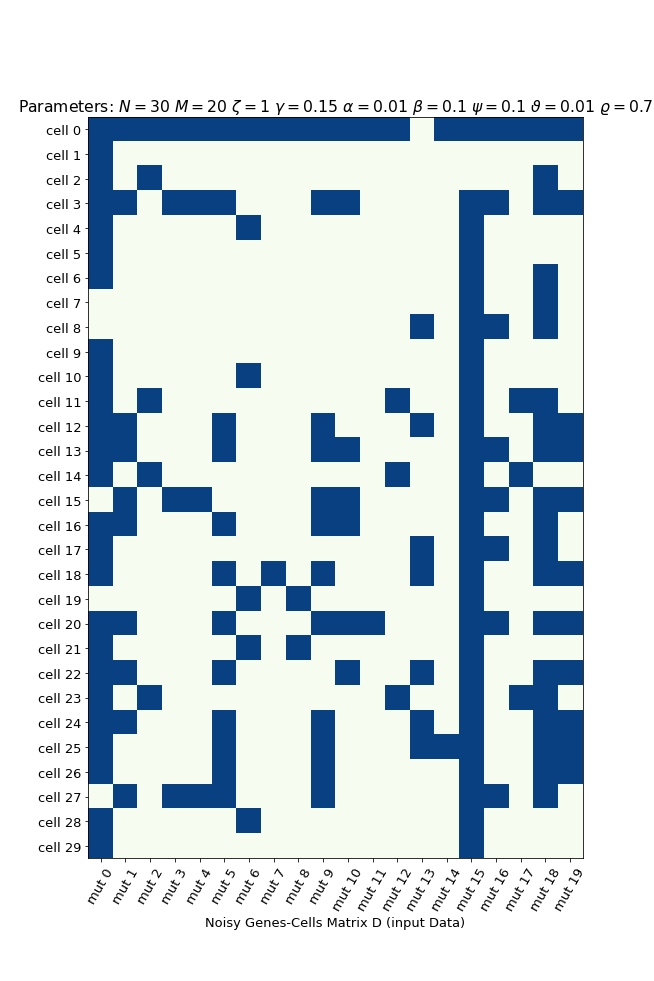
\includegraphics[width=0.32\textwidth]{img/dataset/s/D_zeta=1_gamma=0.15_alpha=0.01_beta=0.1_MR=0.02_N=30_M=20.png}
		\label{fig:D_mt_N30_M20_Z1_G0.15}
	}
	\hfill
	\subfloat[نویزی اضافه شده با پارمترهای $\alpha=0.01, \beta=0.1$]{
		\centering 
		\includegraphics[width=0.32\textwidth]{img/dataset/s/DmE_zeta=1_gamma=0.15_alpha=0.01_beta=0.1_MR=0.02_N=30_M=20.png}
		\label{fig:DmN_mt_N30_M20_Z1_G0.15}
	}
%	\vskip\baselineskip
%	\centering
	\hfill
	\subfloat[ماتریس نویزی به همراه داده‌های از دست رفته با پارامترهای $\alpha=0.1, \beta=0.08, m_r=0.1$]{
		\centering 
		\includegraphics[width=.32\textwidth]{img/dataset/s/Dm_zeta=1_gamma=0.15_alpha=0.01_beta=0.1_MR=0.02_N=30_M=20.png}
		\label{fig:Dm_mt_N30_M20_Z1_G0.15}
	}
	\caption{ماتریس‌های ژن-سلول همراه با نویز و داده‌های از دست رفته شکل \ref{fig:E_mt_N30_M20_Z1_G0.15} که برای ورودی مسئله آماده شده است.}
	\label{fig:D}
\end{figure}


\subsection[پایگاه داده حقیقی]
{پایگاه داده حقیقی
	\LTRfootnote{Real Dataset}
}
به عنوان پایگاه داده حقیقی از پایگاه داده استفاده شده در مقاله \lr{SCITE} به عنوان پایگاه داده حقیقی اصلی استفاده خواهیم کرد \cite{davis2016computing}.

%که ماتریس داده ورودی آن به صورت شکل  \ref{fig:navin_Dm} می‌باشد.
%\begin{figure}[!ht]
%	\centering 
%	\includegraphics[width=0.67\textwidth]{img/dataset/r/Navin_Dm.png}
%	\caption{داده‌های حقیقی \lr{Navin} در مقاله \lr{SCITE}}    
%	\label{fig:navin_Dm}
%\end{figure}

%همچنین پایگاه‌داده حقیقی \lr{Xu} نیز که در مقاله \lr{SCITE} مورد استفاده قرار گرفته است در شکل \ref{fig:Xu_Dm} آمده است.
%\begin{figure}[!ht]
%	\centering 
%	\includegraphics[width=0.625\textwidth]{img/dataset/r/Xu_Dm.png}
%	\caption{داده‌های حقیقی \lr{Xu} در مقاله \lr{SCITE}}    
%	\label{fig:Xu_Dm}
%\end{figure} 

\subsection{آموزش شبکه }
پس از ساخت پایگاه داده مجازی حال می‌توان به آموزش شبکه معرفی شده در \ref{sec:ch_pm:network} پرداخت.
\\
به شکل \ref{fig:ch_er:td3} توجه کنید.
\begin{figure}[!ht]
	\centering 
	\includegraphics[width=\textwidth]{img/chaps/er/td3_crop}
	\caption{نحوه آموزش شبکه با استفاده از ساختار \lr{TD3} \cite{fujimoto2018addressing}.}    
	\label{fig:ch_er:td3}
\end{figure} 

شکل \ref{fig:ch_er:td3} متد ارائه شده در \cite{fujimoto2018addressing} را نمایش می‌دهد که شامل ۱۵ مرحله برای آموزش است که شبکه پیشنهادی خود را به این فرم آموزش دادیم. این مراحل به شرح زیر می‌باشد.
\begin{enumerate}
	\item
ما یک حافظه ۵۰ هزارتایی به عنوان حافظه‌ای از تجربیات انتخاب عمل‌های مختلف\LTRfootnote{Experience replay memory} را در نظر می‌گیریم که در هر انتقال (تکرار) آن را مقداردهی خواهیم کرد.
\item
ساخت یک شبکه برای عملگر مدل (\lr{actor model}) و یک شبکه برای عملگر هدف (\lr{actor target})
\item
ساخت دو شبکه برای نقاد مدل (\lr{critic model}) و دو شبکه برای نقاد هدف (\lr{critic target})
	
\item
در این مرحله یک دسته از انتقال‌های ($s, s', a, r$) را از حافظه انتخاب می‌کنیم. سپس برای هر نمونه از این دسته موارد بعدی را انجام می‌دهیم.
\item
از شرایط حالت بعدی $s'$، عملگر هدف عملیات $a'$ را انجام خواهد داد.
\item
ما یک نویز گوسی (نرمال) به این عملیات بعدی $a'$ اضافه خواهیم کرد و البته نمی‌گذاریم نتیجه حاصله خارج از محدوده قابل قبول قرار بگیرد.
\item
دو شبکه نقاد هدف مقادیر ($s',a'$) را به عنوان ورودی دریافت می‌کنند و در خروجی مقادیر
 \lr{Q-values}، 
$Q_{t1}(s',a')$
 و
 $Q_{t2}(s',a')$
  را تولید می‌کنند.
\item
ما کوچکترین مقدار \lr{Q-values} تولید شده را برمی‌گزینیم: $\min(Q_{t1}, Q_{t2})$. این مقدار در واقع ارزش حالت بعد را تخمین می‌زند.
\item
ما مقدار
$$Q_t=r+\gamma\min(Q_{t1}, Q_{t2})$$
 را از خروجی شبکه‌های نقاد هدف محاسبه می‌کنیم
\item
دو شبکه نقاد مدل مقدار ($s,a$) را دریافت می‌کنند و خروجی‌های 
$Q_1(s,a)$ و $Q_2(s,a)$
 را تولید می‌کنند.
\item
ما مقدار خطا را برای شبکه‌های نقاد مدل به صورت
$$\text{\lr{critic loss = MSE($Q_1, Q_t$)+MSE($Q_2, Q_t$)}}$$
 محاسبه می‌کنیم.
\item
خطای محاسبه شده را برای شبکه‌های نقاد مدل با یک بهینه‌ساز \lr{SDG}، \gls{backpropagate} می‌کنیم
\item
در هر 2 \gls{iteration} یک‌بار، شبکه عملگر مدل را با استفاده از \lr{gradient ascent} بر روی خروجی حاصل از شبکه نقاد مدل اول به صورت
$$\nabla_{\phi}J(\phi)=N^{-1}\Sigma\nabla_aQ_{\theta_1}(s,a)|_{a=\pi_\phi(s)}\nabla_\phi\pi_\phi(s)$$
به روزرسانی می‌کنیم. جایی که $\phi$ و $\theta_1$ به وزن‌های شبکه عملگر و نقاد اشاره می‌کند.
\item
در هر 2 \gls{iteration} یک‌بار، ما وزن‌های شبکه عملگر هدف را به روش \gls{polyakaveraging} به صورت 
$$\theta'_i \leftarrow \tau\theta_i+(1-\tau)\theta'_i$$
به روزرسانی می‌کنیم.
\item
در هر 2 \gls{iteration} یک‌بار، ما وزن‌های شبکه نقاد هدف را به روش \gls{polyakaveraging} به صورت 
$$\phi'_i \leftarrow \tau\phi_i+(1-\tau)\phi'_i$$
 به روزرسانی می‌کنیم.
\end{enumerate}
برای آموزش با توجه نتایجی که در \cite{azer2020tumor} بدست آمده است، یک مرحله پیش‌پردازش را که در آن ماتریس ورودی طبق روش \cite{gusfield1997algorithms} مرتب‌سازی می‌شود را انتخاب می‌کنیم و در ادامه نتایج گزارش‌شده همگی با این پیش‌پردازش خواهند بود.
\\
در ادامه در شکل \ref{fig:ch_er:td3_learning} نتایج آموزش شبکه برای ماتریس‌های با سایز ورودی $15\times 12$ قابل مشاهده است.
\begin{figure}[!ht]
	\subfloat[پارامترهای حذف جهش $\psi=0.1, \vartheta=0.01, \varrho=0.7$]{
		\centering
		\includegraphics[width=0.48\textwidth]{img/chaps/er/net_loss}
		\label{fig:D_mt_N30_M20_Z1_G0.15}
	}
	\hfill
	\subfloat[پارامترهای خطا برابر با $\alpha=0.003, \beta=0.05$]{
		\centering 
		\includegraphics[width=0.48\textwidth]{img/chaps/er/net_acc}
		\label{fig:DmN_mt_N30_M20_Z1_G0.15}
	}
%		\vskip\baselineskip
%		\centering
%%	\hfill
%	\subfloat[ماتریس نویزی به همراه داده‌های از دست رفته با پارامترهای $\alpha=0.1, \beta=0.08, m_r=0.1$]{
%		\centering 
%		\includegraphics[width=.48\textwidth]{img/chaps/er/net_loss}
%		\label{fig:Dm_mt_N30_M20_Z1_G0.15}
%	}
%	\hfill
%	\subfloat[ماتریس نویزی به همراه داده‌های از دست رفته با پارامترهای $\alpha=0.1, \beta=0.08, m_r=0.1$]{
%		\centering 
%		\includegraphics[width=.48\textwidth]{img/chaps/er/net_acc}
%		\label{fig:Dm_mt_N30_M20_Z1_G0.15}
%	}
	\caption{نتیجه آموزش شبکه برای ماتریس‌های ورودی با ابعاد $15\times 12$.}
	\label{fig:ch_er:td3_learning}
\end{figure}



\newpage
\section{نتایج تجربی}
در این بخش به نتایج بدست آمده برای روش پیشنهادی می‌پردازیم و برای هر دو داده مصنوعی و حقیقی نتایج بدست آمده را نمایش خواهیم داد.
\subsection{نتایج بر روی پایگاه داده مصنوعی}
همان‌گونه که در بخش دوم توضیح داده شد با توجه به سختی دسترسی به پایگاه داده‌های حقیقی و اینکه در آن‌ها نیز حقیقت داده‌ها ($E$) وجود ندارد تصمیم به ایجاد پایگاه داده‌ای مصنوعی گرفته شد که با کمک آن بتوان ارزیابی مناسبی از روش پیشنهادی و میزان کارایی و مقاومت روش را نسبت به تغییر پارامترها سنجید.

فرض کنید ماتریس ورودی شکل \ref{fig:sy_D1} را در اختیار داریم و می‌خواهیم بهترین درخت فیلوژنی را برای آن بیابیم.
\begin{figure}[!ht]
	\centering
	\includegraphics[width=0.65\textwidth]{img/chaps/er/s_input_D}
	\caption{نمونه‌ای تصادفی از ماتریس ورودی $D$}
	\label{fig:sy_D1}
\end{figure}

حال یک درخت تصادفی به صورت شکل \ref{fig:sy_initial_T1} می‌سازیم.
\begin{figure}[!ht]
	\centering
	\includegraphics[width=0.8\textwidth]{img/chaps/er/initial_s_tree}
	\caption{‌درخت تصادفی ایجاد شده به عنوان درخت اولیه شکل \ref*{fig:sy_D1}}
	\label{fig:sy_initial_T1}
\end{figure}
در درخت شکل  \ref{fig:sy_initial_T1} نمونه‌ها (سلول‌ها) با رنگ قرمز به درخت متصل شده‌اند که البته این ضمیمه بهترین ضمیمه ممکن است و ضریبی از میزان خطای هر ضمیمه نیز در کادر قرمز رنگ سلول‌ها به صورتی عددی منفی نوشته شده است. 
\\
برای مشاهده خروجی روش پیشنهادی و مقایسه آن با حالت پایه می‌توان نتیجه حاصله برای ماتریس ورودی \ref{fig:sy_D1} را در شکل \ref{fig:sy_benchmark1} مشاهده کرد.



در این شکل دو درخت وجود دارد که درخت سمت راستی درخت حقیقی است که به دنبال آن بودیم و درخت سمت چپ بهترین درخت یافته شده است. همچنین در پایین شکل، ۹ ماتریس مشاهده می‌شود که ماتریس‌ها سمت راست و پایین به نوعی بیان‌کننده میزان خطا بین ۴ ماتریس سمت چپ بالا می‌باشند. در بالای هر ماتریس نام آن نوشته شده است و در نهایت در انتهای تصویر نیز روند کاهش خطا و تلاش‌های روش پایه ما که \lr{SCITE} می‌باشد در گام‌های مختلف قابل مشاهده است. فقط نکته‌ای که وجود دارد این است که خطای نوشته شده در تصاویر برابر ضریبی از خطای اصلی می‌باشد و خود آن نیست.
\\
همان‌گونه که مشخص است در ماتریس $D$ هفت داده از دست رفته وجود دارد که چهار تا از آن‌ها در حقیقت جهش یافته و بقیه خیر. اگر ما در محاسبات خود این هفت داده را در محاسبه خطا در نظر نگیریم و با تغییر ۶ داده دیگر می‌توانیم به ماتریس $\hat{E}$ (در شکل به نام $E$ نوشته شده است) برسیم که معادل بهترین درخت بدست آمده است. که این یعنی ماتریس $D$ ما با بیش از ۴۰ تغییر بدست ما رسیده است. حال اگر حقیقت داده‌ها و درخت اصلی را مشاهده کنیم می‌بینیم که در آنجا فقط ۶ خطا وارد شده است که فقط ۴ مورد از آن‌ها درست کشف شده است و در عوض تعداد بسیار زیادی از داده‌ها را خراب کرده است. بنابرین الگوریتم بدون اطلاع از حقیقت توانسته با  ۴۵ خطا به یک درخت فیلوژنی مناسب دست بیابد. بنابرین روش پایه توانسته درخت فیلوژنی را با صحت 
${15*20 - 45\over15*20} = 0.85\overline{3}$
بازسازی کند که عددی جالبی با توجه به $5000$ تکرار نمی‌باشد.
\begin{figure}[!ht]
	\centering
	\includegraphics[height=0.9\textheight]{img/chaps/er/SCITE_s_tree}
	\caption{‌نتیجه استنتاج درخت فیلوژنی با روش پایه مشابه به مقاله scite برای ماتریس شکل \ref*{fig:sy_D1}}
	\label{fig:sy_benchmark1}
\end{figure}

اما نتیجه روش پیشنهادی خود بر روی همین داده ورودی در شکل \ref{fig:sy_benchmark_pm} قابل مشاهده است. حال اگر به پاسخی که روش ارائه شده برای این ورودی بدست آورده است را دقت کنیم متوجه خواهیم شد که بازسازی نسبت به حالت قبل با دقت بالاتری انجام شده است که هم به صورت چشمی با مقایسه درخت و هم به صورت محاسبه تعداد بازسازی‌های درست که برابر با 
${15*20 - 5\over15*20} = 0.98\overline{3}$
می‌شود، که نشان دهنده مطلوبیت و قدرت روش پیشنهادی است. مخصوصا اگر شکل \ref{fig:sy_benchmark_pm_chart} را مشاهده نمایید و متوجه شوید که برخلاف روش پایه این استنتاج تنها با استفاده از $377$ تکرار انجام شده که دلیل آن همان استفاده از یک شبکه با انتخاب‌های هوشمند در کنار فرض حذف جهش‌های مسافر است. البته باید اذعان کنیم که هر تکرار ما بخاطر بهینه‌سازی‌ای که به ازای هر درخت دارد چندین برابر زمان هر اجرای روش پایه می‌باشد که در قسمت‌های بعدی بیشتر در خصوص این موارد صحبت خواهیم نمود.

\begin{figure}[!ht]
	\centering
	\includegraphics[height=0.85\textheight]{img/chaps/er/PM_s_tree}
	\caption{‌نتیجه استنتاج درخت فیلوژنی با روش پیشنهادی ارائه شده برای ماتریس شکل \ref*{fig:sy_D1}}
	\label{fig:sy_benchmark_pm}
\end{figure}

\begin{figure}[!ht]
\centering
\includegraphics[height=0.25\textheight]{img/chaps/er/PM_s_chart}
\caption{‌نتیجه اجرای روش پیشنهادی ارائه شده برای ماتریس شکل \ref*{fig:sy_D1}}
\label{fig:sy_benchmark_pm_chart}
\end{figure}


\subsubsection{مقایسه دقت بازسازی با توجه به تغییر پارامترها}
برای اینکه بتوانیم ارزیابی مناسب‌تری از روش پیشنهادی داشته باشیم و آن را با حالت پایه مقایسه کنیم در ادامه نتایج اجرا را برای تغییر یکی از پارامترهای اصلی در حین ثابت نگه داشتن بقیه پارامترها آورده‌ایم.\\
در ابتدا با ثابت نگه داشتن تعداد جهش‌ها به افزایش تعداد نمونه‌ها با پذیرش دو جهش به عنوان جهش‌های مسافر و پارامترهای
$\alpha=0.005, \beta=0.03, M=15$
می‌پردازیم که نتیجه بازسازی درخت فیلوژنی به صورت شکل \ref{fig:sy_n_err_mean} می‌باشد.
\begin{figure}[!ht]
	\centering
	\includegraphics[width=0.7\textwidth]{img/chaps/er/comp_pm_scite}
	\caption{‌مقایسه روش پیشنهادی با روش پایه \lr{scite} با پارامترهای $\alpha=0.005, \beta=0.03, M=15$}
	\label{fig:sy_n_err_mean}
\end{figure}
همان‌طور که مشاهده می‌شود، با افزایش تعداد نمونه‌ها ضمن حفظ تعداد جهش‌ها، بازسازی به صورت ‌دقیق‌تری برای هر دو روش همراه است که روش پیشنهادی مشاهده می‌شود با تعداد تکرارهای برابر برای تعداد نمونه‌های یکسان از روش \lr{scite} پاسخ‌های دقیق‌تری ارائه می‌دهد.\\
همچنین تغییر پارامترها و اجرای مجدد خروجی تصویر \ref{fig:ch_er:comp_change_N} را به همراه دارد که در این تصویر، نمودار سمت چپ برابر میانگین خطای فاصله به ازای هر دو ژن در درخت بازسازی شده با درخت واقعی می‌باشد. همچنین در نمودار سمت راست نیز میانگین خطا نمایش داده شده است که این معیار خطا تابعی از خطای اصلی است که برای اینکه در تصاویر به همراه معیار فاصله در یک رنج قرار بگیرند به صورت  
$\left(\left( -\sum\ln(P)\right)/A\right)^{1.3}$ مورد استفاده قرار گرفته است.
\\ در این نمودار نیز کاهش دقت بنظر می‌رسد با سرعت بیشتری برای روش پایه همراه است.
\begin{figure}[!ht]
	\centering
	\includegraphics[width=\textwidth]{img/chaps/er/comp_change_N}
	\caption{‌مقایسه روش پیشنهادی با توجه به تغییر پارامتر $N$}
	\label{fig:ch_er:comp_change_N}
\end{figure}
\noindent
همچنین در نمودارهای تصویر \ref{fig:ch_er:comp_change_M} نتیجه اجرا برای حالتی است که تعداد جهش‌ها در حال افزایش است و نسبت $\frac{M}{N}=1.3$ در تمامی حالات برابر است. دیگر پارامترها بر روی تصویر ذکر شده قابل مشاهده است. در این نمودارها نیز با افزایش ابعاد ماتریس ورودی همچنان روش پیشنهادی نسبت به روش پایه از عملکرد مطلوب‌تری برخوردار است تا زمانی که تعداد جهش‌ها به $30$ می‌رسد که در این زمان خطای روش پایه‌ای بهتر از روش پیشنهادی بود که یکی از دلایل آن می‌تواند به اندازه کافی آموزش ندیدن شبکه باشد اما با این حال با توجه به این نکته که روش پیشنهادی فرض فقدان جهش را در خود دارد توانست همچنان میانگین فواصل بهتری را بین جفت جهش‌ها در درخت حاصل کند.
\begin{figure}[!ht]
	\centering
	\includegraphics[width=\textwidth]{img/chaps/er/comp_change_M}
	\caption{‌مقایسه روش پیشنهادی با توجه به تغییر پارامتر $M$}
	\label{fig:ch_er:comp_change_M}
\end{figure}
\noindent
پس از مشاهده نتایج با توجه به تغییرات تعداد جهش‌ها و نمونه‌ها (ابعاد ماتریس) حال به بررسی تغییرات دیگر پارامترها خواهیم پرداخت. در ادامه نمودار شکل \label{fig:ch_er:comp_change_alpha} تغییرات خطا و میانگین فواصل بین ژن‌ها را با توجه به تغییر پارامتر $\alpha$ نمایش می‌دهد.

\begin{figure}[!ht]
	\centering
	\includegraphics[width=\textwidth]{img/chaps/er/comp_change_alpha}
	\caption{‌مقایسه روش پیشنهادی با توجه به تغییر پارامتر $\alpha$}
	\label{fig:ch_er:comp_change_alpha}
\end{figure}
\noindent
در این شکل با توجه به این‌که مقدار $\alpha$ عدد کوچکی است، تغییرات ایجاد شده توسط آن در ماتریس ورودی برای الگوریتم پیشنهادی نیز به طبع کم تاثیر خواهد بود اما در نهایت با کمی دقت قابل استنتاج است که این افزایش با شیب کمی به افزایش خطا و کاهش دقت منجر خواهد شد.\\
به همین ترتیب نتایج برای تغییرات پارمتر $\beta$ نیز در شکل \ref{fig:ch_er:comp_change_beta} قابل مشاهده می‌باشد.

\begin{figure}[!ht]
	\centering
	\includegraphics[width=0.75\textwidth]{img/chaps/er/comp_change_beta}
	\caption{‌مقایسه روش پیشنهادی با توجه به تغییر پارامتر $\beta$}
	\label{fig:ch_er:comp_change_beta}
\end{figure}
\noindent
اما به جز پارامترها که در روابط مد‌ل‌سازی شده‌اند یکی از مشکلات اصلی وجود داده‌های از دست رفته بود که دو رویکرد برای مدیریت آن‌ها مطرح کردیم. در تصاویر \ref{fig:ch_er:comp_change_MR_pwd} و \ref{fig:ch_er:comp_change_MR_me} نتایج حال از این دو رویکرد نشان داده شده است.

\begin{figure}[!ht]
	\centering
	\includegraphics[width=0.75\textwidth]{img/chaps/er/comp_change_MR_pwd}
	\caption{‌مقایسه روش پیشنهادی با توجه به تغییر پارامتر $MR$ در دقت میانگین فواصل بین جهش‌ها در درخت فیلوژنی}
	\label{fig:ch_er:comp_change_MR_pwd}
\end{figure}
\begin{figure}[!ht]
	\centering
	\includegraphics[width=0.75\textwidth]{img/chaps/er/comp_change_MR_me}
	\caption{‌مقایسه روش پیشنهادی با توجه به تغییر پارامتر $MR$ در مقدار میانگین خطا}
	\label{fig:ch_er:comp_change_MR_me}
\end{figure}
\noindent
همان‌گونه که در این دو تصویر ذکر شده هنگامی که نرخ داده‌های از دست رفته کم است هر دو حالت تقریبا عملکردی مشابه دارند. زیرا که پایین بودن این نرخ به منزله کمتر بودن تعداد داده‌های نامعلوم است که در این تعدادهای کم تفاوت مشخص نیست و خطاهای بوجود آمده نیز در قالب همان پارامترهای $\alpha$ و $\beta$ خود را نشان می‌دهد و مقادیر آن‌ها را نیز برای داده‌ها خراب نمی‌کند. اما رفته رفته هرچه این نرخ افزایش پیدا می‌کند، این اختلاف بیشتر شده و تاثیر خود را در رویکردهای مختلف بازسازی نمایش می‌دهد.

\subsection{نتایج بر روی داده‌های حقیقی}
در نهایت در این بخش روش پیشنهادی خود را بر روی دادگان حقیقی \cite{davis2016computing} اجرا کردیم که نتیجه بدست آمده از آن در شکل \ref{fig:ch_er:pm_tree} قابل مشاهده است.

\begin{figure}[!ht]
	\centering
	\includegraphics[width=0.4\textwidth]{img/chaps/er/pm2}
	\caption{درخت بدست داده‌های حقیقی مورد استفاده مقاله \cite{davis2016computing} توسط روش پیشنهادی}
	\label{fig:ch_er:pm_tree}
\end{figure}
\noindent
پارامترهای مورد استفاده برای این دادگان برابر با $\alpha=0.015$ و $\beta=0.13$ بودند. همچنین نتیجه بدست آمده بهترین نتیجه ممکن برای اجرای 100 بار الگوریتم به ازای ترکیب دو جهش مختلف جهت در مجموعه جهش‌های قابل حذف می‌باشد. ساختار درخت ارائه شده توسط خود مقاله نیز در شکل \ref{fig:ch_er:navin_tree} قابل مشاهده است.

\begin{figure}[!ht]
	\centering
	\includegraphics[width=0.6\textwidth]{img/chaps/er/navin}
	\caption{درخت بدست آمده در مقاله \lr{SCITE}}
	\label{fig:ch_er:navin_tree}
\end{figure}
\noindent
همان‌طور که مشخص است مقدار خطای بدست آمده برای خروجی الگوریتم پیشنهادی بهتر (کمتر) از خطای درخت \lr{SCITE} می‌باشد.
		% فصل پنجم: نتایج تجربی 
% !TeX root=../../../main.tex

\chapter{بحث و نتیجه‌گیری}
% دستور زیر باعث عدم‌نمایش شماره صفحه در اولین صفحهٔ این فصل می‌شود.
%\thispagestyle{empty}

در ابتدا با تعاریف مربوط به حوزه سرطان و دلیل بوجود آمدن آن در بدن فصل اول این پایان‌نامه را آغاز کردیم و در ادامه ارزش و اهمیت این حوزه را بیان کردیم که مطالعات بر روی آن به سرعت درحال گسترش و پیشرفت هستند تا بتوانند با اطلاعات جدیدی که بدست می‌آورند بیش از پیش به نحوه درمان سرطان نزدیک شوند. از این رو ارزش کشف روابط و فیلوژنی بین سلول‌های تومور سرطانی را بازگو کردیم که یکی از مهم‌ترین نیازمندی‌ها برای مواجهه با این بیماری و نحوه پیش‌بینی آن است که اخیرا با معرفی توالی‌یابی‌های تک سلولی به طور چشمگیری دقت مشاهدات جهش‌ها و تغییرات ساختاری بوجود آمده در دی‌ان‌ای سلول‌ها افزایش یافته است. این شرایط فرصت مناسبی را برای کشف ارتباطات این تغییرات با یکدیگر فراهم ساخته است که ما در این پایان نامه به کمک این اطلاعات که شامل اطلاعات جهش‌های تک‌نوکلئوتیدی و تغییرات تعداد کپی بود، مسئله خود را برای استنتاج درخت فیلوژنی شروع کردیم. در فصل دوم به ادبیات موضوعی مورد نیاز پرداختیم و مفاهیم مورد نیاز بین رشته‌ای را که در ادامه به آن‌ها نیاز داشتیم بیان نمودیم.
پس از ان آماده شدیم تا با مرور روش‌های پیشین دریابیم که با یک مسئله \lr{NP-Hard} سرکار داریم که یکی از روش‌های پر استفاده و پایه‌ای آن جست و جو در بین پاسخ‌های ممکن به جای استنباط یکباره پاسخ نهایی است. به همین دلیل در فصل پس از آن روشی را ارائه دادیم که با حفظ همین رویکرد سعی داشت تا ابزارهای جدیدی را به آن اضافه کند تا بتواند با قدرت این ماژول‌های جدید ضمن کاستن از ضعف‌های روش‌های کلاسیک از مزایا و سادگی آن‌ها در حل مسئله استفاده کرد. به همین دلیل دو قسمت را برای تغییر انتخاب کردیم. 
یعنی جایی که برای جست‌وجو تصمیم‌گیری می‌شد و دوم جایی که آن تصمیم و استراتژی از آن نشات می‌گرفت که در واقع آستانه حداکثری را برای دقت و ارزش یک روش مشخص می‌کرد. در روش‌های قبلی جست‌و‌جوها در فضای پاسخ اکثرا یا به صورت تصادفی انجام می‌شد و یا اینکه در بهترین حالت با توجه به فرمولی با قید‌های متفاوت نیازمند یک بهینه‌سازی معمولا سخت برای انتخاب گام بعدی می‌شد. این انواع تصمیم‌گیری در واقع دو لبه تیغ هستند. 
جایی که سرعت با انجام بهینه‌سازی‌هایی که قابلیت گسترش و تعمیم روش را محدود می‌کنند فدای دقت می‌شود و حالت دیگر که بدون هیچ هوشمند‌ی‌ای فقط به دنبال یک تصمیم جدید برای ورود به آن است. ما به دنبال راه حلی بودیم که همزمان بتواند هر دوی این‌ها را داشته باشد. یعنی در عین حال که نمی‌خواهیم درگیر بهینه‌سازی‌های سنگین برای بهترین پاسخ ممکن در هر مرحله شود از طرفی هم مایل به تصمیم‌گیری حریصانه نیستیم. به همین جهت تصمیم گرفتیم تا از ابزار یادگیری تقویتی عمیق برای این منظور بهره گیریم. این ابزار که برای یادگیری و حل مسائل پیچیده بدون درگیر شدن در پیچیدگی‌های آن توسعه یافته است یکی از بهترین انتخاب‌ها برای این منظور بود. به همین جهت این ابزار را در یکی از چارچوب‌های جدید آن که \lr{TD3\LTRfootnote{Twin Delayed DDGP}}است بکار گرفتیم تا بتواند با درنظر گرفتن سیاست مناسب برای رسیدن به یک درخت فیلوژنی با بیشترین درست‌نمایی تصمیمات مناسب در طی گام‌ها اتخاذ کند حتی اگر در این بین مجبور باشد تغییری در درخت بوجود آورد که برای مدت کوتاهی در حالات میانی ساختار درخت را نسبت به پاسخ بهینه دگرگون سازد. برای قسمت بعدی نیز مشاهده کردیم که اطلاعات جدید بدست آمده حاکی از نقص فرض مدل مکان‌های بی‌نهایت است و ممکن است شرایطی در تومور و داده‌های استخراجی از آن‌ها بوجود بیاید که یک جهش بتواند پس از مدتی از بوجود آمدن حذف شود. بنابراین از فرض جدیدی که اجازه می‌داد برخی از جهش‌ها با توجه پروفایل تغییر تعداد کپی در درخت جهش داشته باشند، به جای فرض مدل مکان‌های بی‌نهایت استفاده کردیم که مجموعه جهش‌های با پتانسیل حذف را با توجه به ساختار درخت تشکیل می‌داد. در ادامه در فصل بعد برای ارزیابی روش پیشنهادی و اینکه بتوانیم شبکه خود را آموزش دهیم پایگاه داده‌ای را با پارامترهای متنوعی تعریف کردیم و پس از تشریح نحوه آموزش شبکه به اجرای روش پیشنهادی خود در مقایسه با روش پایه‌ای که تغییرات خود را در آن ایجاد کرده بودیم پرداختیم و نشان دادیم که این تغییرات در روش پایه منجر به افزایش قابل ملاحظه دقت استنتاج درخت فیلوژنی همراه با کاهش گام‌های مورد نیاز برای حصول آن است.
  در ادامه این فصل به بررسی نقاط ضعف و قدرت روش پیشنهادی می‌پردازیم و در انتها پیشنهاداتی را به عنوان کارهایی که می‌توان در ادامه برای بهبود این روش داشت بیان خواهیم نمود.
  
\section{نقاط ضعف و قوت روش پیشنهادی}
  در این قسمت به بررسی نقاط ضعف و قوت روش پیشنهادی می‌پردازیم.
  \\
  همان‌طور که در فصل گذشته مشاهده کردیم روش پیشنهادی قادر بود تا تصمیمات دقیق‌تری را برای ورود به مرحله بعد اتخاذ کند. به همین جهت کاهش خطا و افزایش دقت با سرعت بیشتری انجام می‌شود که نتیجه آن پیمودن گام‌های کمتر برای رسیدن به یک دقت مشخص است. همچنین لحاظ کردن جهش‌هایی که مسافر هستند و پس از مدتی از وقوع‌شان حذف می‌شوند کمک‌کننده این روش است که به اشتباه با اصرار بر فرض مدل مکان‌های بی‌نهایت سعی در تخریب داده‌های درست ماتریس ورودی نداشته باشد و بتواند به این فرض جدید به درختی دست یابد که درست‌نمایی بیشتری را نسبت به حالت روش پایه داشته باشد.
  \\
  اما در خصوص نقض‌های این روش باید گفت به جز مواردی که به عنوان نقطه قوت این روش معرفی شدند نقض‌های روش‌های جست و جو در فضای پاسخ را دارد و این روش هم از این قاعده مستثنی نیست. اما شاید این روش دو ضعف بزرگ نسبت به روش پایه‌ای خود داشته باشد که آن‌ها را در زیربخش بعد بیان خواهیم نمود.
 \subsection{محدودیت‌ها}
  بزرگترین محدودیت این روش همان نقطه قوت این روش است، یعنی شبکه یادگیری تقویتی آن. زیرا که همانظور که وجود آن می‌تواند تصمیمات هوشمندانه را در مدت زمان کوتاهی با استفاده از داد‌ه‌های خام بگیرد، همان‌طور هم اگر این شبکه به طور مناسب آموزش ندیده باشد نمی‌تواند فضای پاسخ را به صورت مناسب تحت پوشش قرار دهد و ممکن است به محلی که پاسخ بهینه در آن قسمت وجود دارد اصلا نزدیک نشود. به همین دلیل وجود همین شبکه یکی از محدودیت‌های این روش است زیرا برای هر تعداد جهش‌ای که مایل به استفاده از داده آن‌ها هستیم لازم است تا شبکه برای آن آموزش ببیند.
  \\
  همچنین طولانی شدن هر تکرار در این روش نسبت به روش پایه یکی دیگر از محدودیت‌های این روش است زیرا همانطور که تعداد گام‌ها را برای رسیدن به یک پاسخ مناسب کوتاه می‌کند اما در عوض در هر مرحله و تکرار برای ساخت بردار $\mathcal{L}$ و چک کردن ژن‌های حذف شونده زمان و انرژی قابل ملاحظه‌ای هزینه می‌شود که بهتر است در روش‌های آینده با ماژولی مناسب‌تر جایگزین شود.
  
  
\section{گام‌های آتی}
در این بخش پیشنهاداتی را برای بهبود روش پیشنهادی ارائه شده بیان خواهیم نمود.\\
در ادامه سه مورد را برای این منظور بیان خواهیم نمود که اولی مربوط به ساخت درخت اولیه، دومی مربوط به استفاده از خود ماژول یادگیری تقویتی به‌جای \lr{MCMC} و سومی ارائه یک راهکار مناسب برای به روزرسانی بردار جهش‌های مسافر به جای بازسازی دوباره آن است.


\subsection{بهبود در ساخت درخت اولیه}
در حال حاضر ما درخت اولیه را به صورت تصادفی انتخاب می‌کنیم که می‌توان در این مرحله درخت اولیه را با استفاده از مفروضات مدل مکان‌های بی‌نهایت و با توجه به ماتریس ورودی بهبود بخشید. این کار باعث می‌شود تا شروع الگوریتم از نقطه بهتری باشد که در این صورت هم گام‌های لازم برای رسیدن به درخت بهینه می‌تواند کمتر شود و هم اینکه احتمال قرار گرفتن در نقاط اکسترمم نسبی را کاهش می‌دهیم.


\subsection{استفاده از ماژول یادگیری تقویتی به‌جای \lr{MCMC} }
در این روش به جای اینکه برای خروجی‌های تولید شده از شبکه یادگیری تقویتی خود شرط پذیرش بگذاریم، می‌توان با تقویت این شبکه و اعتماد به آن تمام پاسخ‌های آن را پذیرفت تا خود این ماژول ما را به سمت درخت بهینه هدایت کند و نه شرایطی که در آن قرار گرفته شده است. این کار اگر میسر شود تعداد گام‌ها همچنان برای حصول درخت فیلوژنی بهینه کاهشی خواهد شد و در این صورت حتی می‌توان امیدوار بود که به جای یک پاسخ بهینه مناسب به بهینه‌ترین پاسخ ممکن دست یافت.

\subsection{ ارائه یک راهکار مناسب برای به روزرسانی بردار $\mathcal{L}$}
یکی از بزرگترین مراحل پر هزینه در این روش پیشنهادی بازتعریف بردار $\mathcal{L}$ به ازای هر تکرار است. این کار هزینه بسیار زیادی دارد و به نوعی در عوض هر چند تعداد گام‌ها برای رسیدن به پاسخ نهایی کمتر می‌شوند اما زمان هر گام به صورت نمایی با افزایش تعداد ژن‌های واجد شرایط حذف افزایش می‌یابد. اما از طرفی می‌دانیم که هر گام در واقع همان درخت قبلی است با یک تغییر و حتما باید راهی وجود داشته باشد که پس از ساخت بردار $\mathcal{L}$ بتوان با توجه به تغییر درخت این بردار را به جای بازتعریف، به روز رسانی کرد. در این صورت ممکن است زمان هر گام بسیار نسبت به حالت فعلی کاهش یابد که در نتیجه می‌توان با همان مقدار زمان و انرژی فضای بزرگتری را برای پاسخ بهینه جست‌وجو کرد که این عمل منجر به کارایی بیشتر روش پیشنهادی خواهد شد.
		% فصل ششم: بحث و نتیجه‌گیری 


% مراجع
% اگر از استیل‌های natbib استفاده می‌کنید باید دو خط را در فایل commands.tex تغییر دهید.
\pagestyle{empty}
{
\small
\onehalfspacing
\bibliographystyle{plain-fa} % or plainnat-fa for author-date
\bibliography{./tex/MyReferences}
}

\pagestyle{fancy}

% \appendix
% فصلهای پس از این قسمت به عنوان ضمیمه خواهند آمد.

% دستورات لازم برای تبدیل «فصل آ» به «پیوست آ» در فهرست مطالب
\addtocontents{toc}{
    \protect\renewcommand\protect\cftchappresnum{\appendixname~}%
    \protect\setlength{\cftchapnumwidth}{\mylenapp}}
    
% دستورات لازم برای شماره‌گذاری صفحات پیوست‌ها بشکل آ-۱ (فعلا با glossaries سازگار نیست)
% \let\Chapter\chapter
%\pretocmd{\chapter}{
%  \clearpage
%  \pagenumbering{arabic}
%  \renewcommand*{\thepage}{\rl{\thechapter-\arabic{page}}}}{}{}
%%%%%%%%%%%%%%%%%%%%%%%%%%%%%%%%%%%%%


%% !TeX root=../main.tex

\chapter{آشنایی سریع با برخی دستورات لاتک}
\label{app:latexIntro}
%\thispagestyle{empty}
در این فصل ویژگی‌های مهم و پرکاربرد زی‌پرشین و لاتک معرفی می‌شود. برای راهنمایی بیشتر و به‌کاربردن ویژگی‌های پیشرفته‌تر به راهنمای زی‌پرشین و راهنمای لاتک مراجعه کنید. برای آگاهی از دستورات لاتک که این خروجی را تولید کرده‌اند فایل \lr{appendix1.tex} را ملاحظه فرمایید.
\footnote{بیشتر مطالب این بخش از مثال 
\lr{xepersian\_example.tex}
گرفته شده‌اند که توسط آقای امیرمسعود پورموسی آماده شده است.}

\section{بندها و زیرنویس‌ها}
هر جایی از نوشتهٔ خود، اگر می‌خواهید به سر سطر بروید و یک بند (پاراگراف) تازه را آغاز کنید، باید یک خط را خالی بگذارید%
\footnote{یعنی دوبار باید کلید \lr{Enter} را بزنید.}
 مانند این:

حالا که یک بند تازه آغاز شده است، یک زیرنویس انگلیسی%
\LTRfootnote{English Footnote!}
 هم می‌نویسیم!
\section{فرمول‌های ریاضی}
\label{formula}

اینجا هم یک فرمول می‌آوریم که شماره دارد:
\begin{equation}\label{eq:yek}
A=\frac{c}{d}+\frac{q^2}{\sin(\omega t)+\Omega_{12}}
\end{equation}
در لاتک می‌توان به کمک فرمان 
\lr{\textbackslash label\{\}}
به هر فرمول یک نام نسبت داد. در فرمول بالا نام \lr{eq:yek} را برایش گذاشته‌ایم (پروندهٔ \lr{tex} همراه با این مثال را ببینید). این نام ما را قادر می‌کند که بعداً بتوانیم با فرمان
\lr{\textbackslash ref\{eq:yek\}}
به آن فرمول با شماره ارجاع دهیم. یعنی بنویسیم فرمول \ref{eq:yek}. 
لاتک خودش شمارهٔ این فرمول‌ها را مدیریت می‌کند.\footnote{یعنی اگر بعداً فرمولی قبل از این فرمول بنویسیم، خودبه‌خود شمارهٔ این فرمول و شمارهٔ ارجاع‌ها به این فرمول یکی زیاد می‌شود. دیگر نگران شماره‌گذاری فرمول‌های خود نباشید!} این هم یک فرمول که شماره ندارد:
$$A=|\vec{a}\times \vec{b}| + \sum_{n=0}^\infty C_{ij}$$

این هم عبارتی ریاضی مانند 
$\sqrt{a^2+b^2}$
 که بین متن می‌آید.
\subsection{یک زیربخش}
\label{zirbakhsh}

این زیربخش \ref{zirbakhsh} است؛ یعنی یک بخش درون بخش \ref{formula} است.
\subsubsection{یک زیرزیربخش}
این هم یک زیرزیربخش است. در لاتک می‌توانید بخش‌های تودرتو در نوشته‌تان تعریف کنید تا ساختار منطقی نوشته را به خوبی نشان دهید. می‌توانید به این بخش‌ها هم با شماره ارجاع دهید، مثلاً بخش فرمول‌های ریاضی شماره‌اش \ref{formula} است.
\section{نوشته‌های فارسی و انگلیسی مخلوط}
نوشتن یک کلمهٔ انگلیسی بین متن فارسی بدیهی است، مانند Example در این جمله.\footnote{هرچند بهتر است باز هم آن کلمه را مانند \lr{Example} در این جمله بنویسید.}
نوشتن یک عبارت چندکلمه‌ای مانند
 \lr{More than one word} کمی پیچیده‌تر است.

اگر ناگهان تصمیم بگیرید که یک بند کاملاً انگلیسی را بنویسید، باید:
\begin{latin}
This is an English paragraph from left to right. You can write as much as you want in it.
\end{latin}
\section{افزودن تصویر به نوشته}
پروندهٔ تصویر دلخواه خود را در کنار پروندهٔ \lr{tex} قرار دهید. سپس به روش زیر تصویر را در نوشتهٔ خود بیاورید:
\begin{latin}
\begin{verbatim}
\includegraphics{YourImageFileName}
\end{verbatim}
\end{latin}
به تصویرها هم مانند فرمول‌ها و بخش‌ها می‌توان با شماره ارجاع داد. مثلاً تصویر \ref{fig:shir} یک شیر علاقه‌مند به لاتک را در حال دویدن نشان می‌دهد. برای جزئیات بیشتر دربارهٔ روش گذاشتن تصویرها در نوشته باید راهنماهای لاتک را بخوانید.
\begin{figure}[ht]
\centerline{\includegraphics[width=5cm]{lion}}
\caption{در این تصویر یک شیر علاقه‌مند به لاتک را در حال دویدن می‌بینید.}
\label{fig:shir}
\end{figure}

به تصویرها هم مانند فرمول‌ها و بخش‌ها می‌توان با شماره ارجاع داد. مثلاً تصویر بالا شماره‌اش \ref{fig:shir} است. برای جزئیات بیشتر دربارهٔ روش گذاشتن تصویرها در نوشته باید راهنماهای لاتک را بخوانید.

\section{محیط‌های شمارش و نکات}
برای فهرست‌کردن چندمورد، اگر ترتیب برایمان مهم نباشد:
\begin{itemize}
\item مورد یکم
\item مورد دوم
\item مورد سوم
\end{itemize}
و اگر ترتیب برایمان مهم باشد:
\begin{enumerate}
\item مورد یکم
\item مورد دوم
\item مورد سوم
\end{enumerate}
می‌توان موردهای تودرتو داشت:
\begin{enumerate}
\item مورد ۱
\item مورد ۲
\begin{enumerate}
\item مورد ۱ از ۲
\item مورد ۲ از ۲
\item مورد ۳ از ۲
\end{enumerate}
\item مورد ۳
\end{enumerate}
شماره‌گذاری این موردها را هم لاتک انجام می‌دهد.

\section{تعریف و قضیه}
برای ذکر تعریف، قضیه و مثال مثالهای ذیل را ببینید.
\begin{definition}
مجموعه همه ارزیابی‌های  (پیوسته)  روی $(X,\tau)$، دامنه توانی احتمالی
\index{دامنه توانی احتمالی}
$ X $
نامیده می‌شود.
\end{definition}
\begin{theorem}[باناخ-آلااغلو]
\index{قضیه باناخ-آلااغلو}
اگر $ V $ یک همسایگی $ 0 $ در فضای برداری 
\index{فضای!برداری}
 توپولوژیکی $ X $ باشد و 
\begin{equation}\label{eq1}
K=\left\lbrace \Lambda \in X^{*}:|\Lambda x|\leqslant 1 ; \ \forall x\in V\right\rbrace,
\end{equation}
آنگاه $ K $،  ضعیف*-فشرده است که در آن، $ X^{*} $ دوگان
\index{فضای!دوگان}
 فضای برداری توپولوژیکی $ X $ است به ‌طوری که عناصر آن،  تابعی‌های 
خطی پیوسته
\index{تابعی خطی پیوسته}
 روی $X$ هستند.
\end{theorem}
تساوی \eqref{eq1} یکی از مهم‌ترین تساوی‌ها در آنالیز تابعی است که در ادامه، به وفور از آن استفاده می‌شود.
\begin{example}
برای هر فضای مرتب، گردایه 
$$U:=\left\lbrace U\in O: U=\uparrow U\right\rbrace $$
از مجموعه‌های بالایی باز، یک توپولوژی تعریف می‌کند که از توپولوژی اصلی، درشت‌تر  است.
\end{example}
حال تساوی 
\begin{equation}\label{eq2}
\sum_{n=1}^{+\infty} 3^{n}x+7x=\int_{1}^{n}8nx+\exp{(2nx)}
\end{equation}
را در نظر بگیرید. با مقایسه تساوی \eqref{eq2} با تساوی \eqref{eq1} می‌توان نتیجه گرفت که ...


\section{چگونگی نوشتن و ارجاع به مراجع}
\label{Sec:Ref}


در لاتک به راحتی می‌توان مراجع خود را نوشت و به آنها ارجاع داد. به عنوان مثال برای معرفی کتاب گنزالس \cite{Gonzalez02book} به عنوان یک مرجع می‌توان آنرا به صورت زیر معرفی نمود:

\singlespacing
\begin{LTR}
\begin{verbatim}
\bibitem{Gonzalez02book}
Gonzalez, R.C., and Woods, R.E. {\em Digital Image Processing}, 3rd ed..
Prentice-Hall, Inc., Upper Saddle River, NJ, USA, 2006.
\end{verbatim}
\end{LTR}
\doublespacing

در دستورات فوق \lr{Gonzalez02book}  برچسبی است که به این مرجع داده شده است و با استفاده از دستور 
\verb!\cite{Gonzalez02book}!
می‌توان به آن ارجاع داد؛ بدون این که شماره‌اش را در فهرست مراجع‌مان بدانیم.

اگر این اولین مرجع ما باشد در قسمت مراجع به صورت زیر خواهد آمد:\\
\includegraphics[width=\textwidth]{gonzalez.png}

این شیوهٔ تعریف مراجع بسیار ابتدایی است و اگر فرمت مراجع، ترتیب یا تعداد آنها را خواسته باشید تغییر دهید، به عنوان مثال ابتدا حرف اول نام نویسنده بیاید و سپس نام خانوادگی، باید همه کارها را به صورت دستی انجام دهید!
چون در یک \پ یا مقاله باید کنترل کاملی بر مراجع خود داشته باشید و به راحتی بتوانید قالب مراجع را عوض کنید، بنابراین می‌بایست از \lr{Bib\TeX} استفاده کنید که درپیوست  \ref{app:refMan} به  آن پرداخته خواهد شد.
		% پیوست اول: آشنایی مقدماتی با لاتک
%% !TeX root=../main.tex

\chapter{‌جدول، نمودار و الگوریتم در لاتک}
\label{app:latex:more}
%\thispagestyle{empty}

در این بخش نمونه مثالهایی از جدول، شکل، نمودار، الگوریتم و معادلات ریاضی را در لاتک خواهیم دید.
دقت کنید که در پایان‌نامه‌ها و مقالات، باید قاعدهٔ «ارجاع به جلو%
\LTRfootnote{Forward Referencing}»
رعایت شود؛ یعنی ابتدا در متن به شمارهٔ شکل، جدول یا معادله اشاره شود و بعد از آن (زیر آن) خود شکل، جدول یا معادله رسم شود. (توضیحات بیشتر در قسمت
\ref{sec:floatObjs}).

\section{جدول}
دستور اصلی برای رسم جدول در لاتک 
\verb|tabular|
می‌باشد که جدول
\eqref{tab:motionModels}
با استفاده از آن کشیده شده است؛ در
\verb|tabular|
عرض جدول برابر با مجموع عرض ستون‌ها و حداکثر مساوی عرض متن است.
\begin{table}[ht]
\caption{مدلهای تبدیل.}
\label{tab:motionModels}
\centering
\onehalfspacing
\begin{tabular}{|r|c|l|r|}
	\hline نام مدل & درجه آزادی & تبدیل مختصات & توضیح \\ 
	\hline انتقالی & ۲ & $\begin{aligned} x'=x+t_x \\ y'=y+t_y \end{aligned}$  &  انتقال دوبعدی\\ 
	\hline اقلیدسی & ۳ & $\begin{aligned} x'=x\cos\theta - y\sin\theta+t_x \\ y'=x\sin\theta+y\cos\theta+t_y \end{aligned}$  &  انتقالی+دوران \\ 
	\hline 
\end{tabular} 
\end{table}

برای اینکه عرض جدول قابل کنترل باشد، باید از دستورات
\verb|tabularx|،
\verb|tabulary| یا
\verb|tabu|
استفاده کرد که راهنمای آنها در اینترنت وجود دارد.
مثلاً جدول
\ref{tab:motionModelsCont}
با
\verb|tabularx|
رسم شده که عرض جدول در آن ثابت بوده و ستون‌های از نوع
\verb|X|
عرض خالی جدول را پر می‌کنند.
\begin{table}[ht]
	\caption{مدلهای تبدیل دیگر.}
	\label{tab:motionModelsCont}
	\centering
	\onehalfspacing
	\begin{tabularx}{\textwidth}{|r|c|l|X|}
		\hline نام مدل & درجه آزادی & تبدیل مختصات & توضیح \\ 
		\hline مشابهت & ۴ & $\begin{aligned} x'=sx\cos\theta - sy\sin\theta+t_x \\ y'=sx\sin\theta+sy\cos\theta+t_y  \end{aligned}$  & اقلیدسی+تغییرمقیاس \\ 		
		\hline آفین & ۶ & $\begin{aligned} x'=a_{11}x+a_{12}y+t_x \\ y'=a_{21}x+a_{22}y+t_y \end{aligned}$  & مشابهت+اریب‌شدگی \\
		\hline
	\end{tabularx}
\end{table}

\section{معادلات ریاضی و ماتریس‌ها}
تقریباً هر آنچه دانشجویان برای نوشتن فرمول‌های ریاضی لازم دارند، در کتاب 
\lr{mathmode}
آمده است. کافیست در خط فرمان، دستور زیر را وارد کنید:
\begin{latin}
	\texttt{texdoc mathmode}
\end{latin}
متن زیر شامل انواعی از اشیاء ریاضی است که با ملاحظه کدش می‌توانید با دستورات آن آشنا شوید.\\
شناخته‌شده‌ترین روش تخمین ماتریس هوموگرافی الگوریتم تبدیل خطی مستقیم (\lr{DLT\LTRfootnote{Direct Linear Transform}}) است.  فرض کنید چهار زوج نقطهٔ متناظر در دو تصویر در دست هستند،  $\mathbf{x}_i\leftrightarrow\mathbf{x}'_i$   و تبدیل با رابطهٔ
  $\mathbf{x}'_i = H\mathbf{x}_i$
  نشان داده می‌شود که در آن:
\[\mathbf{x}'_i=(x'_i,y'_i,w'_i)^\top  \]
و
\[ H=\left[
\begin{array}{ccc}
h_1 & h_2 & h_3 \\ 
h_4 & h_5 & h_6 \\ 
h_7 & h_8 & h_9
\end{array} 
\right]\]
رابطه زیر را برای الگوریتم  \eqref{alg:DLT} لازم داریم.
\begin{equation}
\label{eq:DLT_Ah}
\left[
\begin{array}{ccc}
	0^\top & -w'_i\mathbf{x}_i^\top & y'_i\mathbf{x}_i^\top \\ 
	w'_i\mathbf{x}_i & 0^\top & -x'_i\mathbf{x}_i^\top \\ 
	- y'_i\mathbf{x}_i^\top & x'_i\mathbf{x}_i^\top & 0^\top
\end{array} 
\right]
\left(
\begin{array}{c}
	\mathbf{h}^1 \\ 
	\mathbf{h}^2 \\ 
	\mathbf{h}^3
\end{array} 
\right)=0
\end{equation}

\section{الگوریتم}

\subsection{الگوریتم ساده با دستورهای فارسی}
با مفروضات فوق، الگوریتم \lr{DLT} به صورت نشان داده شده در الگوریتم \eqref{alg:DLT}  خواهد بود.
\begin{algorithm}[ht]
\onehalfspacing
\caption{الگوریتم \lr{DLT} برای تخمین ماتریس هوموگرافی.} \label{alg:DLT}
\begin{algorithmic}[1]
\REQUIRE $n\geq4$ زوج نقطهٔ متناظر در دو تصویر 
${\mathbf{x}_i\leftrightarrow\mathbf{x}'_i}$،\\
\ENSURE ماتریس هوموگرافی $H$ به نحوی‌که: 
$\mathbf{x}'_i = H \mathbf{x}_i$.
  \STATE برای هر زوج نقطهٔ متناظر
$\mathbf{x}_i\leftrightarrow\mathbf{x}'_i$ 
ماتریس $\mathbf{A}_i$ را با استفاده از رابطهٔ \ref{eq:DLT_Ah} محاسبه کنید.
  \STATE ماتریس‌های ۹ ستونی  $\mathbf{A}_i$ را در قالب یک ماتریس $\mathbf{A}$ ۹ ستونی ترکیب کنید. 
  \STATE تجزیهٔ مقادیر منفرد \lr{(SVD)}  ماتریس $\mathbf{A}$ را بدست آورید. بردار واحد متناظر با کمترین مقدار منفرد جواب $\mathbf{h}$ خواهد بود.
  \STATE  ماتریس هوموگرافی $H$ با تغییر شکل $\mathbf{h}$ حاصل خواهد شد.
\end{algorithmic}
\end{algorithm}

\subsection{الگوریتم پیچیده و تودرتو با دستورهای فارسی}
الگوریتم \ref{alg:simulation-random}، یک الگوریتم ترکیبی و تودرتو است که با کمک دستورهای بستهٔ \lr{algorithmic} نوشته شده است.

\begin{algorithm}[p]
    \onehalfspacing
    \caption{الگوریتم اجرای برنامهٔ شبیه‌سازی}
    \label{alg:simulation-random}
    \begin{algorithmic}[1]
        \REQUIRE زمان $t_{max}$ به عنوان زمان لازم برای انجام شبیه سازی،\\
        \REQUIRE  گراف شبکه برای شبیه سازی،
        \ENSURE جدول تغییرات گراف از لحظهٔ ۰ تا t.
        \FOR {تمام لحظات در بازهٔ ۰ تا $t_{max}$}
            \FOR {تمام پیوند‌ها}
                \STATE محاسبهٔ ضریب و نرخ انتقال پیوند
                \STATE محاسبهٔ کیفیت و نرخ یادگیری
            \ENDFOR
            \FOR {تمام گره‌ها}
                \STATE محاسبهٔ نرخ انتقال گره
                \STATE محاسبهٔ وضعیت جدید
            \ENDFOR
            \IF {تغییرات از مقدار $\delta$ کمتر است}
                \STATE شکستن حلقه
                \COMMENT{این شرط برای پایان قبل از رسیدن به محدودیت زمانی است، اگر تغییرات کمتر از $\delta$ باشد}
            \ELSIF {زمان اجرای برنامه بیش از حد طول کشیده \AND $t>100$}
                \STATE شکستن حلقه
            \ENDIF
        \ENDFOR
        \PRINT {زمان اجرای برنامه}
        \RETURN {ماتریس تغییرات زمانی}
    \end{algorithmic}
\end{algorithm}

\subsection{الگوریتم با دستورهای لاتین}
الگوریتم \ref{alg:RANSAC} یک الگوریتم با دستورهای لاتین است.

\begin{algorithm}[ht]
\onehalfspacing
\caption{الگوریتم \lr{RANSAC} برای تخمین ماتریس هوموگرافی.} \label{alg:RANSAC}
\begin{latin}
\begin{algorithmic}[1]
\REQUIRE $n\geq4$ putative correspondences, number of estimations, $N$, distance threshold $T_{dist}$.\\
\ENSURE Set of inliers and Homography matrix $H$.
\FOR{$k = 1$ to $N$}
  \STATE Randomly choose 4 correspondence,
  \STATE Check whether these points are colinear, if so, redo the above step
  \STATE Compute the homography $H_{curr}$ by DLT algorithm from the 4 points pairs,
  \STATE $\ldots$ % الگوریتم کامل نیست
  \ENDFOR
  \STATE Refinement: re-estimate H from all the inliers using the DLT algorithm.
\end{algorithmic}
\end{latin}
\end{algorithm}

\section{کد}
درج کد به زبان‌های مختلف به سادگی امکان‌پذیر است. برنامه
\ref{code:matlabEx}
یک قطعه کد
\lr{MATLAB}
را نشان می‌دهد.
\begin{figure}[ht]
	\begin{LTR}
        \singlespacing
		\lstinputlisting[language=MATLAB, caption={نمونه کد \lr{MATLAB}}, label={code:matlabEx}]{MatlabExample.m}
        % \doublespacing
	\end{LTR}
\end{figure}

\section{تصویر}
نمونهٔ یک تصویر را در فصل قبل دیدیم. دو تصویر شیر کنار هم را نیز در شکل
\ref{fig:twoLion}
مشاهده می‌کنید.
\begin{figure}[ht]
\centering 
\subfloat[شیر ۱]{ \label{fig:twolion:one}
\includegraphics[width=0.3\textwidth]{lion}}
%\hspace{2mm}
\subfloat[شیر ۲]{ \label{fig:twolion:two}
\includegraphics[width=0.3\textwidth]{lion}}%
\caption{دو شیر}
\label{fig:twoLion} %% label for entire figure
\end{figure}

\section{نمودار}
لاتک بسته‌هایی با قابلیت‌های زیاد برای رسم انواع مختلف نمودارها دارد. مانند بسته‌های \lr{Tikz} و  \lr{PSTricks}. توضیح اینها فراتر از این پیوست کوچک است.%
\footnote{
مثال‌هایی از بکارگیری بسته
\lr{Tikz}
را می‌توانید در
\url{http://www.texample.net/tikz/examples/}
ببینید. توصیه می‌شود دانشجویانی که قصد درج اشکالی مانند گراف را در سند خود دارند، مثالهایی از سایت مذکور را ملاحظه فرمایند.
}
یک نمودار رسم شده با بستهٔ 
\lr{TikZ}
 در شکل 
\ref{fig:parabola}
نشان داده شده است.
\begin{figure}[t]
\centering
\begin{tikzpicture}[scale=2.5]
  \shade[top color=blue,bottom color=gray!50] 
      (0,0) parabola (1.5,2.25) |- (0,0);
  \draw (1.05cm,2pt) node[above] 
      {$\displaystyle\int_0^{3/2} \!\!x^2\mathrm{d}x$};

  \draw[style=help lines] (0,0) grid (3.9,3.9)
       [step=0.25cm]      (1,2) grid +(1,1);

  \draw[->] (-0.2,0) -- (4,0) node[right] {$x$};
  \draw[->] (0,-0.2) -- (0,4) node[above] {$f(x)$};

  \foreach \x/\xtext in {1/1, 1.5/1\frac{1}{2}, 2/2, 3/3}
    \draw[shift={(\x,0)}] (0pt,2pt) -- (0pt,-2pt) node[below] {$\xtext$};

  \foreach \y/\ytext in {1/1, 2/2, 2.25/2\frac{1}{4}, 3/3}
    \draw[shift={(0,\y)}] (2pt,0pt) -- (-2pt,0pt) node[left] {$\ytext$};

  \draw (-.5,.25) parabola bend (0,0) (2,4) node[below right] {$x^2$};
\end{tikzpicture}
\caption{یک نمودار زیبا با ارقام فارسی و قابلیت بزرگ‌نمایی بسیار، بدون از دست دادن کیفیت.}
\label{fig:parabola}
\end{figure}

\section{نحوه قرارگیری اشیای شناور}
\label{sec:floatObjs}
شکل‌ها، جداول و الگوریتم‌ها در لاتک اشیای شناور محسوب می‌شوند؛ یعنی خود لاتک تصمیم می‌گیرد آنها را در کجای صفحه ترسیم کند تا زیباتر باشد. اما می‌توان به لاتک توصیه کرد که آن را در قسمت خاصی از صفحه رسم کند. برای اینکه قاعدهٔ «ارجاع به جلو» رعایت شود باید فقط از پرچم
\verb|[ht]|
استفاده کرد، که می‌گوید اگر جا شد شکل را دقیقاً در همین مکان و در غیراینصورت در بالای صفحه بعد رسم کن.
بنابراین دستورات درج تصویر، جدول و الگوریتم به صورت زیر باید باشند:

\begin{latin}
\begin{verbatim}
	\begin{figure/table/algorithm}[ht]
		...
	\end{figure/table/algorithm}
\end{verbatim}
\end{latin}
		% پیوست دوم: جدول، نمودار و الگوریتم در لاتک
%% !TeX root=../main.tex
\chapter{مراجع، واژه‌نامه و حاشیه‌نویسی}
\label{app:refMan}
%\thispagestyle{empty}

\section{مراجع و نقل‌قول‌ها}
\label{sec:refUsage}
منابعِ پایان‌نامه، پایه و اساس تحقیق شما به حساب می‌آیند و ضرورت انجام مطالعه و روش‌های به کار رفته در بسیاری از قسمت‌های آن، به کمک منابع صورت می‌گیرد. در استفاده از مراجع علمی در پایان‌نامه، باید سعی کنید بیشتر از
\textbf{منابع چاپ‌شده و مهم}
استفاده کنید و
\emph{ارجاع به داده‌های چاپ نشده، خلاصه‌ها و پایان‌نامه‌ها، سبب به‌هم‌خوردگی و کاهش اعتبار قسمت ارجاع منابع می‌شود.}
استفاده از منابع و نقل قول‌هایی به تحقیق شما ارزش می‌دهند که
\textbf{در راستای هدف تحقیق بوده و به آن اعتبار ببخشند.}
برخی از دانش‌جویان تصوّر می‌کنند که کثرت نقل‌قول‌ها و ارجاعات زیاد، مهم‌ترین معیار علمی شدن پایان‌نامه است؛ حال آنکه استناد به تعداد کثیری از منابع بدون مطالعه دقیق آنها و استفادهٔ مستقیم در پایان‌نامه، می‌تواند نشان‌دهندهٔ عدم احساس امنیت نویسنده باشد!

دو روش برای استفاده از نتایج، جملات، داده‌ها و روش‌های دیگران وجود دارد. یکی نقل‌قول مستقیم و دقیق است و دیگری استفاده غیرمستقیم در متن مقاله، که در ادامه به قواعد این دو نوع نقل‌قول و ارجاع‌دهی اشاره می‌کنیم:
\begin{description}
	\item[نقل‌قول مستقیم:]
	نقل‌قول مستقیم باید دقیق و بدون هیچ تغییری در جملات باشد. بهتر است این‌گونه نقل‌قول‌ها تا حد امکان کوتاه باشد. جملات کوتاه داخل گیومه قرار می‌گیرند و باید به منبع دقیق آن، طبق روش ارجاع‌دهی به منابع، اشاره شود. به عنوان مثال در
	\cite{persianbib87userguide}
	آمده است که:
	\begin{quote}
		«با استفاده از فیلد
		\lr{AUTHORFA}
		می‌توان معادل فارسی نام نویسندگان مقالات لاتین را در متن داشت. معمولاً در اسناد فارسی خواسته می‌شود که پس از ذکر معادل فارسی نام نویسنده، نام لاتین نویسنده(ها) به عنوان پاورقی درج شود
		\citep{persianbib87userguide}.»
	\end{quote}
	\item[نقل‌قول غیرمستقیم:]
	نقل‌قول غیرمستقیم به معنی استفاده از ایده‌ها، نتایج، روش‌ها و داده‌های دیگران در درون متنِ پایان‌نامه، ولی به سبک خودتان و متناسب و هماهنگ با روند پایان‌نامهٔ شماست. در این حالت نیز باید متناسب با شیوهٔ ارجاع‌دهی به آن استناد شود.
\end{description}

با توجه به وجود سبک‌های مختلف ارجاع‌دهی، باید
\textbf{روش قابل قبول و یکسانی}
در طول پایان‌نامه برای اشاره به مراجع در متن و همچنین تهیه فهرست مراجع در انتهای پایان‌نامه بکار رود. مثلاً برای پایان‌نامه‌های مهندسی می‌توان از سبک ارجاع‌دهی
\lr{IEEE}%
\LTRfootnote{\url{http://www.ieee.org/documents/ieeecitationref.pdf}}
یا
\lr{acm}
استفاده کرد. طبیعتاً باید تناظر یک‌به‌یک بین فهرست مراجع در انتهای گزارش و مراجع مورد استفاده در متن باشد%
\footnote{البته گاهی ممکن است محقق مرجعی را مورد مطالعه قرار داده لیکن در متن به آن اشاره نکرده باشد؛ برخی معتقدند در این موارد نیز آوردن آن در فهرست مراجع، اشکالی ندارد، به این شرط که از عنوان «فهرست منابع» به جای «فهرست مراجع» استفاده شود.}.

برای سهولت مدیریت مراجعِ \پ%
، اکیداً توصیه می‌شود از یک ابزار «مدیریت منابع» (با خروجی
\texorpdfstring{\lr{Bib\TeX}}{Bib\TeX}%
) همچون
\lr{Mendeley}،
\lr{Zotero},
\lr{EndNote}
یا
\lr{Citavi}
استفاده کنید.

\subsection{ مدیریت مراجع با  \texorpdfstring{\lr{Bib\TeX}}{Bib\TeX}}
در بخش \ref{Sec:Ref} اشاره شد که با دستور 
 \lr{\textbackslash bibitem}
  می‌توان یک مرجع را تعریف نمود و با فرمان
 \lr{\textbackslash cite}
  به آن ارجاع داد. این روش برای تعداد مراجع زیاد و تغییرات آنها مناسب نیست. برای مدیریت منابع زیاد، سه بستهٔ
\lr{BibTeX} (پیش‌فرض),
\lr{natbib}
(ارجاع‌دهی در متن به صورت نویسنده-سال)
و \lr{BibLaTeX} (جدید و منعطف‌پذیر)
وجود دارند. در ادامه توضیحاتی در مورد مدیریت منابع با \lr{BibTeX} و \lr{natbib} در زی‌پرشین خواهیم آورد که همراه با توزیع‌های معروف تِک عرضه می‌شوند
\footnote{روش \lr{BibLaTeX} هنوز برای متون فارسی به درستی ترجمه نشده است.}.

یکی از روش‌های قدرتمند و انعطاف‌پذیر برای نوشتن مراجعِ مقالات و مدیریت مراجع در لاتک، استفاده از  \lr{BibTeX} است.
 روش کار با بیب‌تک به این صورت است که مجموعهٔ همهٔ مراجعی را که در \پ استفاده کرده یا خواهیم کرد، 
در پروندهٔ جداگانه‌ای با پسوند
\lr{bib}
نوشته و به آن فایل در سند خودمان به صورت مناسب لینک می‌دهیم.
 کنفرانس‌ها یا مجله‌های گوناگون برای نوشتن مراجع، قالب‌ها یا قراردادهای متفاوتی دارند که به آنها استیل‌های مراجع گفته می‌شود.
 در این حالت به کمک ‌استیل‌های بیب‌تک خواهید توانست تنها با تغییر یک پارامتر در پروندهٔ ورودی خود، مراجع را مطابق قالب موردنظر تنظیم کنید. 
 بیشتر مجلات و کنفرانس‌های معتبر یک فایل سبک
 (\lr{BibTeX Style})
با پسوند \lr{bst} در وب‌گاه خود می‌گذارند که برای همین منظور طراحی شده است.

به جز نوشتن مقالات، این سبک‌ها کمک بسیار خوبی برای تهیهٔ مستندات علمی همچون پایان‌نامه‌هاست که فرد می‌تواند هر قسمت از کارش را که نوشت مراجع مربوطه را به بانک مراجع خود اضافه نماید. با داشتن چنین بانکی از مراجع، وی خواهد توانست به راحتی یک یا چند ارجاع به مراجع و یا یک یا چند بخش را حذف یا اضافه ‌نماید؛ 
مراجع به صورت خودکار مرتب شده و
\textbf{فقط مراجع ارجاع داده شده در قسمت کتاب‌نامه خواهندآمد.}
قالب مراجع به صورت یکدست مطابق سبک داده شده بوده و نیازی نیست که کاربر درگیر قالب‌دهی به مراجع باشد. 

\subsection{سبک‌های مورد تأیید دانشگاه تهران}
طبق «دستورالعمل نگارش و تدوین پایان‌نامه» دانشگاه تهران در
\cite{UTThesisGuide}،
ارجاع در متن می‌تواند مطابق با هر یک از دو الگوی هاروارد یا ونکوور باشد:
\singlespacing
\begin{description}
	\item[سیستم نویسنده-سال (هاروارد):]
	ذکر نام نویسنده و سال نشر در متن. در این الگو مراجع بر اساس حروف الفبا تنظیم می‌گردند.
	\item[سیستم شماره‌دار (ونکوور):]
	ارجاع به مراجع به کمک شماره در متن. در این الگو شماره هر مرجع به ترتیب ظاهر شدن آن در متن در داخل کروشه قرار می‌گیرد. فهرست مراجع نیز بر اساس شماره مرجع (نه حروف الفبا) تنظیم می‌گردد.
\end{description}
\doublespacing

در مدیریت منابع با
\lr{\textbf{BibTeX}}،
ارجاع‌ها در متن تنها به شکل
\textbf{شماره‌دار (ونکوور)}
امکان‌پذیر است، گرچه فهرست مراجع می‌تواند با روش‌های مختلف مرتب شود. اگر بخواهیم ارجاع‌ها در متن به صورت
\textbf{نویسنده-سال (هاروارد)}
باشد باید از بستهٔ
\lr{\textbf{natbib}}\LTRfootnote{Natural Sciences Citations \& References}
و استیل‌های مختلف آن استفاده کنیم.

هنگام استفاده از روش نویسنده-سال نوع پرانتزگذاری‌ها در وسط و انتهای جمله با هم فرق خواهد داشت. به مثال زیر مطابق با دستورالعمل
\cite{UTThesisGuide}
توجه کنید:

\textit{
ابتدا
\cite{Khalighi87xepersian}
بستهٔ زی‌پرشین را برای حروف‌چینی فارسی اختراع کرد. بعدها سبک‌های ارجاع‌دهی فارسی و قالب‌های پایان‌نامه نیز مبتنی بر آن ساخته شد
\citep{persianbib87userguide}.
ارجاع‌دهی به مراجع لاتین نیز در زی‌پرشین امکان‌پذیر است. مثلاً
\citelatin{Gonzalez02book}
یک کتاب انگلیسی است و به راحتی به مقالات انگلیسی نیز می‌توان ارجاع داد
\citeplatin{kim2016integrated}.}

در این مثال، ۴ ارجاع در وسط و انتهای جمله به مراجع فارسی و انگلیسی آمده است. وقتی از سیستم نویسنده-سال استفاده می‌کنید، بهتر است ارجاع‌های آخر جمله کلاً داخل پرانتر بیاید؛ بدین منظور باید به جای
\verb|\cite|
از
\verb|\citep|
استفاده کنید. اما در سیستم شماره‌دار چون تمام ارجاع‌ها داخل کروشه می‌آیند این امر اهمیت ندارد.\\
نمی‌توانید در متن فارسی، اسم لاتین محقق خارجی را بیاورید و برای جلوگیری از ایجاد ابهام، صرف‌نظر از نام لاتین هم مجاز نیست! توصیه می‌شود که نام محقق خارجی در متن با حروف فارسی و در پاورقی اسم تمام نویسندگان به صورت انگلیسی آورده شود. نحوهٔ رعایت این نکته را می‌توانید در کد مثال بالا ببینید.

گرچه در تمپلت ورد
\cite{UTThesisGuide}،
به صراحت ذکر شده که بهتر است برای پایان‌نامه‌های مهندسی از سبک 
\lr{IEEE}
استفاده شود (که از سیستم ونکوور تبعیت می‌کند)، اما ترتیب فهرست مراجع در
\lr{IEEE}
بر اساس ترتیب ارجاع در متن بوده و
\emph{مراجع انگلیسی و فارسی از هم تفکیک نمی‌شوند}
که متضاد با دستورالعمل
\cite{UTThesisGuide}
و نیز متضاد عرف اکثر پایان‌نامه‌های فارسی است.
بنابراین دقیقاً نمی‌توان سبک خاصی را برای مراجع پایان‌نامه‌های دانشگاه تهران اجبار کرد. مهم این است که
\textbf{سبک ارجاع‌دهی در تمام طول یک کتابچه}
(مثلاً پایان‌نامه، مقالات یک مجله یا کل یک کتاب) یکسان باشد. بهتر است
\textbf{بسته به حوزه پایان‌نامه}،
در این مورد با استاد راهنمای خود مشورت کنید.

\subsection{سبک‌های فارسی قابل استفاده در زی‌پرشین}
تعدادی از سبک‌های فارسی بسته
\lr{Persian-bib}%
\footnote{ برای اطلاع بیشتر به راهنمای بستهٔ
\lr{Persian-bib}
مراجعه فرمایید.}
که برای  زی‌پرشین آماده شده‌اند، عبارتند از:

\singlespacing
\begin{itemize}
\item \emph{سبک‌های شماره‌دار}:
	\begin{description}
	\item [unsrt-fa.bst] این سبک متناظر با \lr{unsrt.bst} می‌باشد. مراجع به ترتیب ارجاع در متن ظاهر می‌شوند.
	\item [plain-fa.bst] این سبک متناظر با \lr{plain.bst} می‌باشد. مراجع بر اساس نام‌خانوادگی نویسندگان، به ترتیب صعودی مرتب می‌شوند.
	 همچنین ابتدا مراجع فارسی و سپس مراجع انگلیسی خواهند آمد.
	\item [acm-fa.bst] این سبک متناظر با \lr{acm.bst} می‌باشد. شبیه \lr{plain-fa.bst} است.  قالب مراجع کمی متفاوت است. اسامی نویسندگان انگلیسی با حروف بزرگ انگلیسی نمایش داده می‌شوند. (مراجع مرتب می‌شوند)
	\item [ieeetr-fa.bst] این سبک متناظر با \lr{ieeetr.bst} می‌باشد. (مراجع مرتب نمی‌شوند)
	\end{description}
	
\item \emph{سبک‌های نویسنده-سال}:
	\begin{description}
	\item [plainnat-fa.bst] این سبک متناظر با \lr{plainnat.bst} می‌باشد. نیاز به بستهٔ \lr{natbib} دارد. (مراجع مرتب می‌شوند)
	\item [chicago-fa.bst] این سبک متناظر با \lr{chicago.bst} می‌باشد. نیاز به بستهٔ \lr{natbib} دارد. (مراجع مرتب می‌شوند)
	\item [asa-fa.bst] این سبک متناظر با \lr{asa.bst} می‌باشد. نیاز به بستهٔ \lr{natbib} دارد. (مراجع مرتب می‌شوند)
	\end{description}
\end{itemize}
\doublespacing

با استفاده از استیل‌های فوق می‌توانید به انواع مختلفی از مراجع فارسی و لاتین ارجاع دهید.
به عنوان مثال‌هایی از
\textbf{مراجع انگلیسی}،
مرجع
\cite{Baker02limits}\footnote{چون فیلد \lr{authorfa} برای این مرجع تعریف نشده در سبک نویسنده-سال با حروف لاتین به آن در متن ارجاع می‌شود که غلط است.}
مقالهٔ یک ژورنال، مرجع
\cite{Amintoosi09video}
مقالهٔ یک کنفرانس، مرجع
\citelatin{Gonzalez02book}
یک کتاب، مرجع
\cite{Khalighi07MscThesis}
پایان‌نامهٔ کارشناسی ارشد و مرجع
\citelatin{Borman04thesis}
یک رسالهٔ دکتری می‌باشد.\\
همچنین در میان
\textbf{مراجع فارسی},
مرجع
\cite{Vahedi87}
مقالهٔ یک مجله، مرجع
\cite{Amintoosi87afzayesh}
مقالهٔ یک کنفرانس، مرجع
\cite{Pedram80osool}
یک کتاب ترجمه‌شده با ذکر مترجمان و ویراستاران، مرجع
\cite{Pourmousa88mscThesis}
پایان‌نامهٔ کارشناسی ارشد%
\footnote{همان‌طور که در بخش
\ref{sec:refUsage}
اشاره شد، بهتر است زیاد از پایان‌نامه‌ها در مراجع استفاده نکنید.}،
مرجع
\cite{Omidali82phdThesis}
یک رسالهٔ دکتری و مراجع
\cite{persianbib87userguide, Khalighi87xepersian}
نمونه‌های متفرقه هستند.

\subsection{ساختار فایل مراجع}
برای استفاده از بیب‌تک باید مراجع خود را در یک فایل با پسوند \lr{bib} ذخیره نمایید. یک فایل \lr{bib} در واقع یک پایگاه داده از مراجع%
\LTRfootnote{Bibliography Database}
شماست که هر مرجع در آن به عنوان یک رکورد از این پایگاه داده
با قالبی خاص ذخیره می‌شود. به هر رکورد یک مدخل%
\LTRfootnote{Entry}
گفته می‌شود. یک نمونه مدخل برای معرفی کتاب \lr{Digital Image Processing} در ادامه آمده است:

\singlespacing
\begin{LTR}
\begin{verbatim}
@BOOK{Gonzalez02image,
  AUTHOR     = {Gonzalez,, Rafael C. and Woods,, Richard E.},
  TITLE      = {Digital Image Processing},
  PUBLISHER  = {Prentice-Hall, Inc.},
  YEAR       = {2006},
  ISBN       = {013168728X},
  EDITION    = {3rd},
  ADDRESS    = {Upper Saddle River, NJ, USA}
}
\end{verbatim}
\end{LTR}
\doublespacing

در مثال فوق، \lr{@BOOK} مشخصهٔ شروع یک مدخل مربوط به یک کتاب و \lr{Gonzalez02book} برچسبی است که به این مرجع منتسب شده است.
 این برچسب بایستی یکتا باشد. برای آنکه بتوان
\textbf{برچسب مراجع}
 را به راحتی به خاطر سپرد و حتی‌الامکان برچسب‌ها متفاوت با هم باشند، معمولاً از قوانین خاصی به این منظور استفاده می‌شود. یک قانون می‌تواند
\textbf{فامیل نویسنده اول + دورقم سال نشر + اولین کلمهٔ عنوان اثر}
باشد. به
\lr{AUTHOR}، \lr{TITLE}، $\dots$ و \lr{ADDRESS}
فیلدهای این مدخل گفته می‌شود، که هر یک با مقادیر مربوط به مرجع پر شده‌اند. ترتیب فیلدها مهم نیست. 

انواع متنوعی از مدخل‌ها برای اقسام مختلف مراجع همچون کتاب، مقالهٔ کنفرانس و مقالهٔ ژورنال وجود دارد که برخی فیلدهای آنها با هم متفاوت است. 
نام فیلدها بیانگر نوع اطلاعات آن می‌باشد. مثالهای ذکر شده در فایل \lr{MyReferences.bib} کمک خوبی برای شما خواهد بود. 
%این فایل یک فایل متنی بوده و با ویرایشگرهای معمول همچون \lr{Notepad++} قابل ویرایش می‌باشد. برنامه‌هایی همچون 
%\lr{TeXMaker}
% امکاناتی برای نوشتن این مدخل‌ها دارند و به صورت خودکار فیلدهای مربوطه را در فایل \lr{bib}  شما قرار می‌دهند.  
با استفاده از سبک‌های فارسی آماده شده، محتویات هر فیلد می‌تواند به فارسی نوشته شود؛ ترتیب مراجع و نحوهٔ چینش فیلدهای هر مرجع را سبک مورد استفاده  مشخص خواهد کرد.

\textbf{در فایل 
\lr{MyReferences.bib}
 که همراه با این \پ هست، مثال‌های مختلفی از مراجع آمده‌اند که برای درج مراجع خود، تنها کافیست مراجع‌تان را جایگزین موارد مندرج در آن نمایید.
}

برای بسیاری از مقالات لاتین حتی لازم نیست که مدخل مربوط به آنرا خودتان بنویسید. با جستجوی 
\textbf{نام مقاله + کلمه
\lr{bibtex}}
در اینترنت سایت‌های بسیاری همچون
\lr{ACM} و \lr{ScienceDirect}
را خواهید یافت که مدخل
\lr{bibtex}
مربوط به مقاله شما را دارند و کافیست آنرا به انتهای فایل
\lr{MyReferences.bib}
اضافه کنید.

\subsection{نحوه اجرای \texorpdfstring{\lr{Bib\TeX}}{Bib\TeX}}
پس از قرار دادن مراجع خود، برای ساخت فایل خروجی می‌توانید دستور زیر را (در ترمینال یا از طریق \lr{Texmaker}) اجرا کنید:%
\footnote{فایل \lr{latexmkrc} باید در کنار \lr{main.tex} وجود داشته باشد.}

\singlespacing
\begin{LTR}
	\begin{verbatim}
		latexmk -bibtex -pdf main.tex
	\end{verbatim}
\end{LTR}
\doublespacing
ابزار \lr{latexmk} مراحل مختلف ساخت خروجی لاتک را به طور خودکار و بهینه انجام می‌دهد و هر بار فقط مراحلی را که لازم باشد تکرار می‌کند.
روش دستی‌تر این است که یک بار \lr{XeLaTeX} را روی سند خود اجرا نمایید، سپس \lr{bibtex} و پس از آن هم ۲ بار \lr{XeLaTeX} را. در \lr{TeXMaker} کلید \lr{F11} و در \lr{TeXWorks} هم گزینهٔ \lr{BibTeX} از منوی \lr{Typeset}، \lr{BibTeX} را روی سند شما اجرا می‌کنند.

\section{واژه‌نامه‌ها و فهرست اختصارات}
\gls{Gloss}
یا فرهنگ لغات، مجموعه‌ای از اصطلاحات و تعاریف خاص و فنی است که معمولاً در انتهای یک کتاب می‌آید. چون پایان‌نامه خود یک متن تخصصی بلند محسوب می‌شود، استفاده از فرهنگ لغات در انتهای آن به شدت توصیه می‌شود، خصوصاً که احتمال استفاده از لغات تخصصی لاتین در آن بالاست.
واژه‌نامه‌هایی که در انتهای کتاب‌های انگلیسی می‌آیند معمولاً تک‌زبانه هستند و معنی یک اصطلاح تخصصی در آنها، عمدتاً به صورت یک
\gls{Description}
طولانی آورده می‌شود. اما چون در متون فارسی، آوردن لغات انگلیسی مجاز نیست و باید معادل فارسی آنها وارد شود، جهت رفع ابهام معمولاً واژه‌نامهٔ فارسی به انگلیسی (و برعکس) در انتهای کتاب درج شده و  
\glspl{Description}
در صورت نیاز در متن آورده می‌شوند.

فهرست
\glspl{Acronym}
شامل نمادهای کوتاهی است که اغلب از حروف ابتدایی کلمات یک عبارت طولانی ساخته شده‌اند. با اینکه
\glspl{Acronym}
با حروف (بزرگ) لاتین نوشته می‌شوند، اما چون کوتاهند استفاده از آنها در میان متن فارسی مجاز است. با این حال برای رفع ابهام، عرف است که فهرستی از آنها شامل معنی هر نماد، در کنار دیگر فهرست‌ها در ابتدای متن درج شود.

در این قالب پایان‌نامه، برای ساخت و مدیریت واژه‌نامه و فهرست اختصارات از بستهٔ پیشرفتهٔ
\lr{glossaries}
با موتور واژه‌نامه‌سازی
\lr{xindy}
استفاده می‌شود. تنظیمات بهینهٔ این بسته در فایل
\lr{glossaries-settings.tex}
عبارتند از:
\begin{itemize}
	\item
قبل از درج واژه‌ها در متن، باید مدخل آنها با دستور زیر (ترجیحاً در فایل جدای \lr{words.tex}) تعریف شود:
	\begin{LTR}
	\verb|\newword{Label}{Word}|\{واژه\}\{واژه‌ها\}
	\end{LTR}
	
	\item
قبل از وارد کردن علائم اختصاری در متن، باید مدخل آنها نیز (ترجیحاً در فایل \lr{acronyms.tex}) به صورت زیر تعریف شود:
	\begin{LTR}
	\verb|\newacronym{Label}{Acr}|\{معنی‌اختصار\}
	\end{LTR}

	\item
جهت درج یک علامت اختصاری یا معادل یک واژه تخصصی، کافی است از دستور
	\verb|gls{Label}|
در متن استفاده کنید. دستور
	\verb|glspl{Label}|
نیز برای آوردن معادل یک لغت در حالت جمع ساخته شده است.
	
	\item
هنگام اولین استفاده از یک معادل فارسی یا اختصار در متن، معادل انگلیسی یا معنی آن در پاورقی آورده می‌شود. در صورتی که هر یک از این پیش‌فرض‌ها را دوست ندارید با ویرایش فایل
	\lr{glossaries-settings.tex}
می‌توانید آن را تغییر دهید.

	\item
در انتهای پایان‌نامه با دستور
\verb|\printglossary|
فهرست کلمات استفاده‌شده به ترتیب الفبای فارسی (واژه‌نامه فارسی به انگلیسی) و الفبای انگلیسی (واژه‌نامه انگلیسی به فارسی) درج می‌شود.
\end{itemize}

به عنوان مثال، با مشاهدهٔ کد این نوشته، نحوهٔ درج معادل فارسی
\gls{RandomVariable}
را در متن مشاهده می‌کنید.
در نمایش واژهٔ
\gls{RandomVariable}
برای بار دوم، معادل لاتین در پاورقی نمی‌آید.
در مورد درج علائم اختصاری، مثلاً می‌توان به رابطهٔ
\gls{F}
اشاره کرد.

\section{حاشیه‌نویسی در نسخه پیش‌نویس}
اصلاح و بازبینی چندین و چندبارهٔ یک پایان‌نامه یا مقاله، از معمول‌ترین امور در نگارش آن می‌باشد. فرض کنید دانشجو پایان‌نامه یا مقالهٔ خود را (کامل یا ناقص) نوشته و می‌خواهد نظر استاد راهنما، اعضای آزمایشگاه یا دیگر متخصصین را در مورد آن جویا شود. به جز مشاورهٔ حضوری، تلفنی یا از طریق ایمیل، برای اظهارنظر دقیق بر نوشته، می‌توان از ابزارهای حاشیه‌نویسی در فایل
\lr{PDF}
یا \lr{tex}
نیز استفاده کرد.

یک راهکار مناسب برای حاشیه‌نویسی در فایل \lr{tex}، استفاده از بسته 
\lr{todonotes}
می‌باشد که آقای خلیقی به تازگی امکان استفاده از آن را برای فارسی‌زبانان نیز فراهم آورده‌اند.
بدین منظور، هر جایی که خواستید نکته یا نکاتی را در حاشیه متن یادداشت کنید، کافی است دستور زیر را وارد نمایید:
\begin{latin}
\verb|\todo{NOTE}|
\end{latin}
مثلاً استاد راهنما می‌تواند از دانشجو بخواهد که در بخشی توضیح بیشتری دهد.
\todo{
توضیح بیشتری لازم است.
}
استاد راهنما یا داور حتی می‌تواند محل پیشنهادی برای درج یک تصویر را نیز به راحتی برای دانشجو مشخص کند.
\missingfigure[figwidth=\textwidth,figcolor=white]{یک تصویر از خروجی الگوریتم 
\ref{alg:RANSAC}
را در اینجا قرار دهید.}
یکی دیگر از امکانات این بسته آن است که می‌توان فهرست نکات را در ابتدای سند داشت. بسته 
\lr{todonotes}
امکانات بسیاری دارد
\todo[fancyline,color=green!30]{مرجع این مطلب؟}
که در راهنمای آن معرفی شده است و با اجرای دستور زیر در خط فرمان می‌توانید آنها را مشاهده کنید:
\begin{latin}	
	\texttt{texdoc todonotes}
\end{latin}	
دقت کنید که توضیحات حاشیه‌ای و فهرست کارهای باقیمانده (نکات)،
\textbf{فقط در نسخه
\gls{Draft}}
قابل دیدن هستند و در نسخه نهایی، نمایش داده نخواهند شد.
برای استفاده از حالت
\gls{Draft}
باید گزینه 
\lr{draft}
به دستور 
\verb|\documentclass|
در ابتدای فایل 
\lr{main.tex}
اضافه شود.
هنگامی‌که سند شما در حالت 
\gls{Draft}
باشد:

\singlespacing
\begin{enumerate}
\item 
هیچ یک از صفحات آغازین پایان‌نامه، تا فهرست مطالب نمایش داده نمی‌شود (به جز صفحه اول).
\item
روی صفحه اول عبارت «پیش‌نویس» به صورت درشت و کم‌رنگ نمایش داده می‌شود.
\item
فهرست نکات درج شده توسط
\lr{todo}،
پس از فهرست اصلی و با عنوان «فهرست کارهای باقیمانده» نمایش داده می‌شود.
\item
شماره صفحاتی که به هر مرجع ارجاع داده شده است در بخش مراجع نمایش داده می‌شود
\footnote{اعمال گزینهٔ
\lr{pagebackref}
برای بستهٔ
\lr{hyperref}.
}.
\end{enumerate}
\doublespacing
هر یک از موارد بالا تا زمانی که نسخه نهایی \پ نیاز نباشد بسیار مورد توجه و مفید واقع می‌شوند.
   	% پیوست سوم: مراجع، واژه‌نامه و حاشیه‌نویسی

% برگرداندن شماره‌بندی صفحات فصول
% \let\chapter\Chapter
\pagenumbering{tartibi} % اول، دوم، ...
%\baselineskip=.75cm

% چاپ واژه‌نامه‌ها و نمایه 
\onehalfspacing
\cleardoublepage
\printglossary
\cleardoublepage
\printindex

\begin{latin}
	\baselineskip=.6cm
	\latinabstract
	\latinTitlePage
\end{latin}
\label{LastPage}

\end{document}
